\documentclass[12pt,a4paper,twoside,openright]{book}

%%%%%%%%%%%%%%%%%%%%%%%%%%%%%%%%%%%%%%%%%%%%%%%%%%%%%%%%%%%%%%%%%%%%
%  Template per Tesi di Laurea                                     %
%                                                                  %
%%%%%%%%%%%%%%%%%%%%%%%%%%%%%%%%%%%%%%%%%%%%%%%%%%%%%%%%%%%%%%%%%%%%

               %%%%%%%%%%%%%%%%%%%%%%%%%%%%%%%%%%%%%%
               %    Scelta dei package da usare     %
               %%%%%%%%%%%%%%%%%%%%%%%%%%%%%%%%%%%%%%
\usepackage{macros}


               %%%%%%%%%%%%%%%%%%%%%%%%%%%%%%%%%%%%%%
               %  Scelta del tipo di font da usare  %
               %%%%%%%%%%%%%%%%%%%%%%%%%%%%%%%%%%%%%%

%\usepackage{times,mathptm}
%\usepackage{palatino,mathpple}
%\usepackage{bookman}
%\usepackage{newcent}

               %%%%%%%%%%%%%%%%%%%%%%%%%%%%%%%%%%%%%%%%
               % Scelta delle dimensioni della pagina %
               %%%%%%%%%%%%%%%%%%%%%%%%%%%%%%%%%%%%%%%%

\setlength{\textwidth}{16.0cm}
\setlength{\textheight}{21cm}
\setlength{\footskip}{3cm}



               %%%%%%%%%%%%%%%%%%%%%%%%%%%%%%%%%%%%%%
               %  Informazioni generali sulla Tesi  %
               %    da usare nell'intestazione      %
               %%%%%%%%%%%%%%%%%%%%%%%%%%%%%%%%%%%%%%

\titolo{Engineering complex computational ecosystems}
\candidato{Danilo Pianini}
\annoaccademico{2015}
\facolta{Ingegneria}
\dipartimento{DEIS - Dipartimento di Elettronica, Informatica e Sistemistica}
\dottorato{PhD Course in Electronics, Computer Science and Telecommunications}
\settoreconcorsuale{09/H1}
\settoredisciplinare{ING-INF/05}
\ciclo{XXVII}
\tutor{Antonio Natali}
\relatore{Mirko Viroli}
% \correlatoreb{Andrea Roli}
% \correlatorec{Mirko Viroli}
\coordinatore{Alessandro Vanelli Coralli}
\dedica{
\begin{flushright}
\textit{Considerate la vostra semenza:\\
fatti non foste a viver come bruti,\\
ma per seguir virtute e canoscenza.}
\end{flushright}

\noindent \emph{\textbf{Acknowledgements}}\\ \\

Most of the material that got integrated as a single work in this thesis has been written in publications of which I am co-author.
%
I am thankful to those great researchers I have collaborated with, for their suggestions, their guidance and their help.
%
I'd like to thank first Mirko Viroli, who supervised me for the past three years and tried to make me a scientist.
%
Sara Montagna, which shares the APICe laboratory with me, also deserves a special mention.
%
I want to thank the work packages leaders of SAPERE, a European project that kickstarted me in the world of research: Franco Zambonelli, Giovanna di Marzo, Simon Dobson, Marco Mamei, Alois Ferscha (that also supervised me for three months in Linz) and Andrea Omicini.
%
A special thank to Jacob ``Jake'' Beal, that supervised (and also hosted) me during my last three months in the United States.
%
Finally, I desire to thank these other great researchers and professionals I have collaborated with: Bernhard Anzengruber, Jose-Luis Fernandez Marquez, Stefano Mariani, Ronaldo Menezes, Jussi Nieminen, Matteo Risoldi, Stefano Sebastio, Graeme Stevenson, Andrea Vandin, Sascia Virruso, Juan ``Erica'' Ye.}

\data{\today}

\signature{\emph{Danilo Pianini}}

              %%%%%%%%%%%%%%%%%%%%%%%%%%%%%%%%%%%%%%
               % Fine Preambolo                     %
               % Inizio tesi                        %
               %%%%%%%%%%%%%%%%%%%%%%%%%%%%%%%%%%%%%%

\begin{document}

%%%%%%%%%%%%%%%%%%%%%%%%%
% inizio prefazione
%
% pagina del titolo, indice, sommario
%%%%%%%%%%%%%%%%%%%%%%%%%
\frontmatter
\maketitle
\pagestyle{plain}

\tableofcontents

\chapter*{\centering Abstract}
\addcontentsline{toc}{chapter}{Abstract}

This work presents advancements of the latest three years in the engineering techniques for self-organising pervasive ecosystems of devices and services.
%
The inherent complexity of such systems poses new challenges to those who try to dominate the complexity by applying the principles of engineering.

The recent growth in number and distribution of devices with decent computational and communicational abilities, that got suddenly accelerated with the massive diffusion of smartphones and tablets, is envisioning a world with a much higher density of devices in space.
%
This already high device density is probably going to consistently rise if the diffusion of wearable devices gets momentum.
%
Also, communication technologies seem to be focussing on short-range device-to-device (P2P) interactions, with technologies such as \btle{} and Near-Field Communication getting more and more diffused.

Locality and situatedness become key to provide the best possible experience to users, and the classic model of a centralised, enormously powerful server gathering data and processing it is likely to get less and less efficient with device density.
%
Accomplishing complex global tasks without a centralised controller responsible of aggregating data from devices, however, still is a challenging task.
%
In particular, it is hard to understand which device-local programs could properly interact and guarantee a certain global service level.
%
Such local-to-global issue makes the application of engineering principles challenging at least.

In this work, I lay the foundations of my contribution by first analysing the state of the art in coordination systems, namely in those software frameworks devoted to control and promote interactions among independent software entities.
%
I then motivate my work, by describing the main issues of pre-existing tools and practices and identifying the improvements that would benefit the design of such complex software ecosystems.
%
My contribution can be divided in three main branches:
\begin{enumerate}
 \item a novel simulation tool-chain for pervasive ecosystems;
 \item introduction of novel and improvements over existing self-organisation patterns;
 \item creation of a new language and interpreter based on ``field calculus'' and its integration with the previously mentioned tool
\end{enumerate}
%
Finally, I draw conclusions and future works.

\mainmatter

% stile della pagina
\pagestyle{fancy}
\fancyhead[LE,RO]{\bfseries\thepage}

\part{Background and Motivation}
\label{background}
\chapter{Pervasive computing}
\label{pervasive-devices}

It is no mystery that, with the huge progresses of miniaturisation, computational-capable devices are populating the world.
%
The diffusion got momentum with affordable ``personal computers'' that made their way in a one-device-per-family world.
%
Laptops boosted the process, offering user a personal and mobile device.

The pervasive revolution, however took place when the phones became ``smart'', and with the subsequent improvements in the communication technologies.
%
In this\levelText{} I try to briefly walk the path of success of personal mobile devices, describing also the probable newcomer, namely the wearable devices.
%
I also focus on the current status of the communication protocols, their range and usage, and I try to foresee which world are we going to build if the current trend continues.

\section{Smart, portable devices}

\begin{figure}
	\centering
	
\includegraphics[width=\textwidth]{img/iphone}
	\caption[Apple iPhone]{Apple iPhone is one of the first devices without any physical keyboard, and the first smartphone to gain worldwide success. \emph{Source: Wikimedia.}}
	\label{img:iphone}
\end{figure}

When Apple in 2007 released the first iPhone (\Cref{img:iphone}), a mobile revolution started.
%
Even though other manufacturers proposed products similar to iPhone under the point of view of communication technologies and computational capabilities in the same time frame (e.g. Nokia N810), the Apple's smartphone was the first gaining widespread adoption.
%
It is not really relevant for this work to understand if the branding, the design, the multi-touch finger based interaction UI or the feature set was the key of its commercial success: what really matters is that, starting 2007, every person began to carry with her a personal device featuring both the abilities to communicate and compute.
%
The reason, besides the success of iPhone in the higher segment of the phone market, is mainly to attribute to the widespread diffusion of similar but cheaper and less powerful devices in the lower segments.
%
This kind of devices ultimately pushed the market share of the dominating today's mobile operating system, Google's Android.

This trend towards a higher diffusion got another leap forward three years later, in 2010, when a device with a feature set similar to iPhone, but with no phone abilities  and a bigger screen was released: the iPad.
%
As iPhone gave new vitality and perspectives to the phone arena, iPad revitalised a market that was languishing: the tablets.
%
Tablet devices as they were conceived before iPad launched were nothing more than small laptops with a screen that could be rotated or detached from the keyboard, and a touch-screen normally used with the help of a pen.
%
They changed from devices designed for a professional niche to widespread tools, up to the point that Gartner forecasts their shipments to overtake in 2015 those of desktop PC and laptops aggregated \footnote{\url{http://www.gartner.com/newsroom/id/2791017}}.

The new frontier of pervasive is probably the wearable technology. Smartphones were precursors, they substituted mobile phones introducing new features and they have potential to substitute our wallets (see, for instance, payments through NFC technology) and keys, becoming the only object we need to carry with us in our pockets.
%
Still there are other accessories which are hard to replace, above all watches and glasses.
%
Yes, smartphone can easily show the current time accurately (and, to be honest, also feature phones had this feature well before 2007), but they require the user to pick them from the pocket, turn them on, and sometimes, depending on privacy settings, also unlock them.
%
The whole operation, takes a much longer time and higher effort with respect to just rotating a wrist.
%
This might be the reason why, despite the explosive expansion of smartphones, the wristwatches market did not declined, as an analysis from MarketWatch points out \footnote{\url{http://www.marketwatch.com/story/the-watchs-time-isnt-up-2013-07-01}}.

\begin{figure}
	\centering
	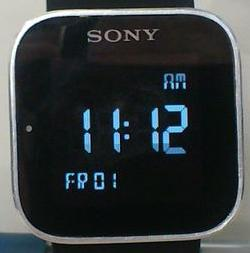
\includegraphics[height=5cm]{img/sony-sw}
	
\includegraphics[height=5cm]{img/samsung-gg}
	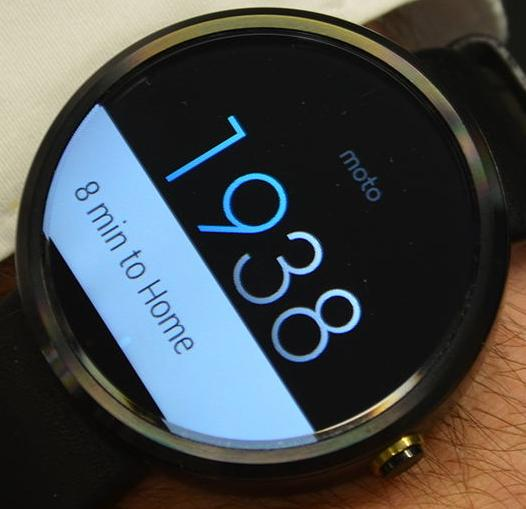
\includegraphics[height=5cm]{img/moto360}
	\caption[Smart watches]{Smart watches. From left to right: Sony Smartwatch \emph{(Source: Alex S.H. Lin)}, Samsung Galaxy Gear \emph{(Source: Karlis Dambrans)}, Motorola Moto 360.}
	\label{img:watches}
\end{figure}

There is room for manufacturers to create new portable devices.
%
Sony, starting 2012, has produced a series of smartwatches, such as those in \Cref{img:watches} that pair with a smartphone and provide quick access to some of its functionalities.
%
The success of such solution is not huge, but despite that many other companies are interested in this market: Samsung, Motorola and Apple presented devices meant to replace the classic wristwatch, a clear sign that this market is in expansion.
%
At the time of writing, the main issues that slow the widespread adoption of such solutions are battery duration and dependence on a smartphone.

\begin{figure}
	\centering
	
\includegraphics[width=0.7\textwidth]{img/gglass}
	\caption[Google Glass]{Google Glass. In this image, it is possible to see both the camera (on the left hand side) and the semi-transparent head-mounted display. Are those devices going to be part of our everyday life? \emph{Source: Wikimedia.}}
	\label{img:gglass}
\end{figure}

Another notable attempt to make a common accessory smarter is Google Glass project, depicted in \Cref{img:gglass}.
%
Their goal is to enhance the experience of wearing glasses by attaching a device with a camera, an optical head-mounted display, and the abilities to locate itself and communicate with other devices.
%
Google Glass, at the time of writing, are way to expensive (with the kit sold at \$1500) for being able to penetrate the general public, but they are an interesting anticipation of possible future devices.

On the same line of such wearable devices, a discrete success is being achieved by the so called ``fit bands''.
%
They are bracelets equipped with low energy sensors, mainly accelerometers and gyroscopes, which are used to keep track of user's activity.
%
Depending on the model, they can be used to monitor some user's health parameters, such as the number of steps walked per day or heartbeats.
%
They normally work along with another device, a smartphone or a tablet.
%
Such devices, due to their precise market niche and reasonably low price (the Chinese manufacturer Xiaomi recently introduced a low-end wristband at around \$15) are having a notable success.

The wearable devices segment also includes less common devices such as ``smart shoes'' and materials that can be used to make clothing, such as e-textiles.
%
It is a market in expansion, greatly beneficing from recent increases in performance per watt efficiency.
%
If the trend continues, it is likely that we will more and more powerful wearable devices on sale at cheaper and cheaper prices, and a consequent widespread diffusion.
%
The same sort may occur to other parts of our life: kitchen gear, indoor lights and many other objects are getting more and more ``smart'' around us.
%
We may, literally, end up with a world where every single object embeds computational and communicational abilities.

A problem arise: how can software engineers deal with such a complexity?

\section{Communication technologies}

Besides miniaturisation, and as a consequence the increase of computational density in space, another factor played a fundamental role in the world of pervasive computing: the ability to communicate, and in particular the ability to rely on wireless communication, which is of paramount importance when considering mobility.

In later years, many communication means arose.
%
They largely differ in terms of range, protocols, and availability.
%
In this\levelText{}I try to resume the most diffused technologies available on today's devices, but the reader is warned: keep in mind that such technologies are evolving very quickly, and the scenario is incredibly fluid.

\subsection{International Mobile Telecommunications}
\label{International Mobile Telecommunications}

This first mean of communication is designed to allow mobile devices to access the Internet from anywhere in the world, relying on the existing mobile phone infrastructure.
%
Such technologies are meant to be used with the standard IP protocols, and they are normally used to get access to public services, in particular to the world wide web.
%
They are not designed for a local peer-to-peer (P2P) communication, and as a consequence they provide no mean to exploit locality.
%
The diffusion of such communication protocols is widespread, in particular among smartphones.
%
Due to the fact that they rely on the mobile phone network, they require a contract with a mobile telecommunications provider, and as such they are much less diffused in tablets and other portable devices.

\begin{figure}
	\centering
	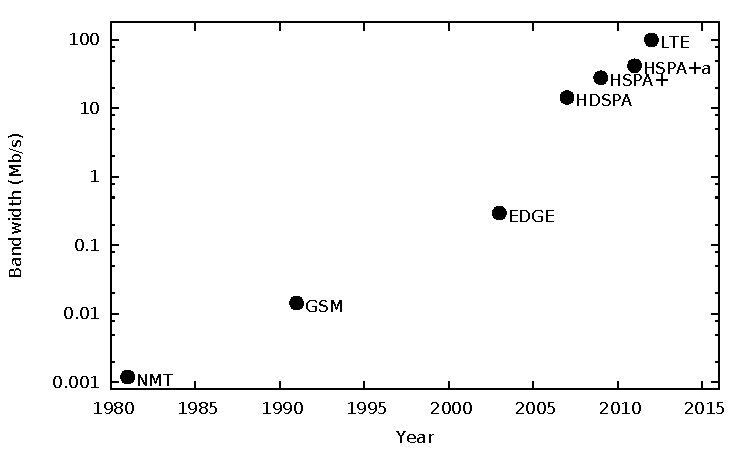
\includegraphics[width=0.99\textwidth]{img/charts/mobile-data-performance}
	\caption[Bandwidth of international mobile telecommunications services]{
		Maximum download bandwidth available for mobile devices with time.
		%
		Each point is labelled with the specific communication technology name.
		%
		For the most recent multiple-input-multiple-output (MIMO) technologies, such as LTE, a conservative single input channel was used.
	}
	\label{img:mobile-bandwidth}
\end{figure}

The possibility of accessing the Internet from everywhere is probably one of the key bricks that allowed for the huge success of smartphones in today's world.
%
As \Cref{img:mobile-bandwidth} shows, the bandwidth available grew exponentially with time, to the point that in some countries (e.g. in Italy, at the time of writing) the best available mobile connections offer a higher performance than the best available home connection
%
\footnote{At the time of writing, Telecom Italia Mobile offers mobile connections on LTE with a download bandwidth up to 225Mb/s.
%
Fastweb, the company offering the faster solutions for fiber-to-home connections, goes up to 100Mb/s.}.
%
Such performance unlock the possibility of fully exploiting the possibilities of the world wide web, including cloud services and fruition of multimedia content.

If bandwidth is not currently an issue for international mobile telecommunications, the situation is well different when it comes to device density.
%
Any of us probably experienced network availability issues when participating crowded events, such as concerts or sport events.
%
The current technology, in fact, makes all the network user share the same physical resources: when the device density is too high, there is simply not enough space in the frequency spectrum to grant a decent bandwidth to everyone.
%
Future networks (5G, and presumably those that will follow) are focussing toward this issue among others \cite{5g}.
%
In particular, a so-called ``spectrum crunch'' is expected due to the expected traffic increase (thousand fold over this decade and still growing into the next), that could not be faced simply with the foreseen steady increase of the spectrum allocated for mobile communication, and will require technological advances \cite{spectrum-crunch}.

\subsection{WiFi}

WiFi technology is the most diffused technology for wireless local networking.
%
It is widely diffused, integrated in all smartphones and tablets and also in other devices, such as printers, gaming consoles and TVs.
%
WiFi devices communicate on a distance that ranges from 20 to 100 meters, depending on the condition of the wireless medium and on the power of the communication devices.
%
The communication speed between two linked devices ranges from 56Mb/s to 300Mb/s.

WiFi was designed to provide wireless access to a local area network.
%
In the most classic ``infrastructure mode'', wireless devices get connected to a so called access point, which is responsible to route packets among wireless devices and bridge the wireless local area network to the wired backbone.
%
Multiple access point that share the network name (SSID) may be connected using wired network technologies, and they will appear as a single, bigger access point.
%
It is also possible to drop the wired backbone, but specific access points are required.

Also, some WiFi devices provided ``ad-hoc mode'', allowing multiple devices to directly communicate without an intermediate access point.
%
This working mode was problematic, mainly due to the fact a standard communication protocol for peer-to-peer WiFi communication was missing.
%
This lack was filled with WiFi Direct, which provides a protocol by which one of the devices that want to communicate directly becomes the access point, allowing for direct communication.
%
The most common usage of such a feature are direct file sharing between devices and connection to peripheral devices such as printers or scanners.

\subsection{Bluetooth and Bluetooth LE}

Bluetooth is a technology designed for building energy efficient personal area networks (PANs).
%
Bluetooth devices are assigned a class which identifies the maximum permitted power and, consequently, the maximum operating range.
%
For the most powerful (and power hungry) devices the communication range can go up to 100m.
%
The communication speed ranges from 1Mb/s of the earliest 1.0 version to the 24 Mb/s of version 3.0 and later.

The most interesting features of Bluetooth are not the bandwidth nor the range (WiFi performs better on both), but rather the simple association process and the low power consumption.
%
Thanks to those features Bluetooth found widespread diffusion as a mean to connect low consumption peripherals, such as headsets.
%
Also, it is diffused in cars, and allows user to use the car's audio system as a speakerphone for making calls or listen to music.

\begin{figure}
	\centering
	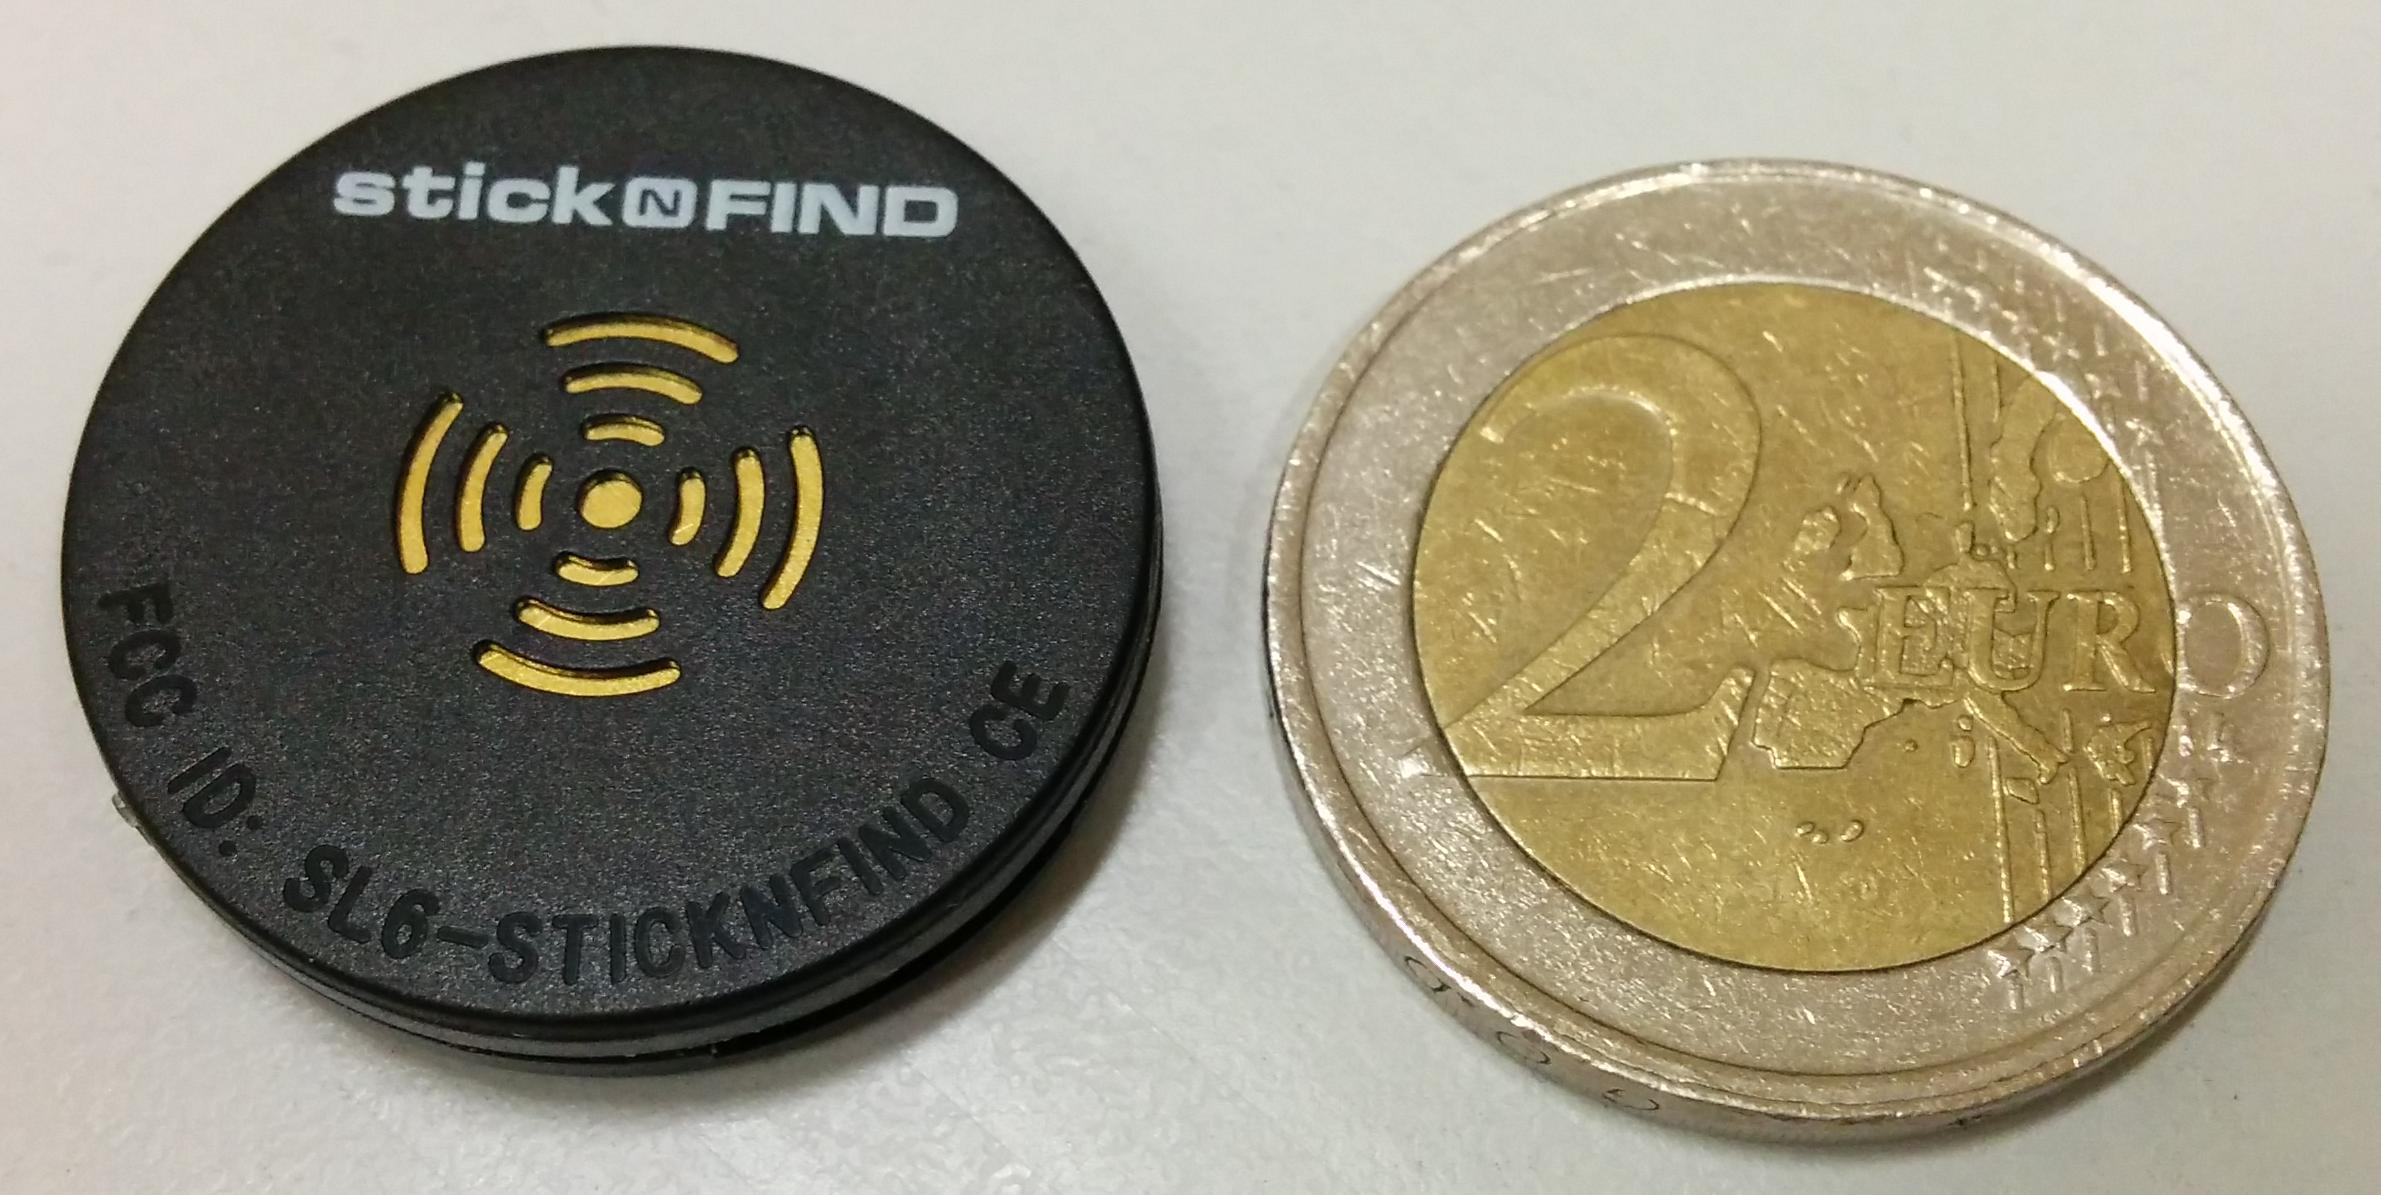
\includegraphics[width=0.99\textwidth]{img/ibeacon}
	\caption[iBeacon]{
		A iBeacon, compared to a \EUR{2} coin.
	}
	\label{img:ibeacon}
\end{figure}

A technology which is often associated with Bluetooth but that is actually a separated and not compatible protocol is Bluetooth LE.
%
The reason why such technologies get associated is that, since the radio frequency used is the same (2.4GHz), dual mode devices can share a single radio antenna.
%
LE stands for Low Energy, and it is the main difference between the two protocols: at the expense of some bandwidth, Bluetooth LE consistently reduce the amount of energy required.
%
Bluetooth LE applications are particularly interesting, and range from health care to fitness to alerts to proximity sensing.

Proximity can be estimated using the received signal strength indicator (RSSI), and the very low power consumption of Bluetooth LE allowed for the realisation of electronic leashing systems, namely systems where an electronic device is paired to an object and can be used in order to compute the relative position.
%
The applications are, for instance, finding of misplaced, out-of-sight devices (when the electronic device is paired with a movable object) and indoor localisation (if the electronic device is located on a still standing object).
%
Relying on this technology, Apple created iBeacon, namely very small (coin sized, see \Cref{img:ibeacon}) electronic devices consisting basically of a battery and a Bluetooth LE device.
%
iBeacons can be attached to objects, and they send a universally unique identifier (UUID) to enabled smartphones in range.
%
If the smartphone can associate the UUID with a position, it can deduce its location relative to the iBeacon.
%
The low energy feature plays a fundamental role in this kind of applications: beacons whose battery would last few hours would be of little practical use.
%
With current technologies, a beacon device can be powered by a standard, rather cheap battery for several months, up to a couple of years.
%
This technology is probably the prelude to precise indoor localisation. 

\subsection{NFC}

\begin{figure}
	\centering
	
\includegraphics[width=0.99\textwidth]{img/nfc-tag}
	\caption[NFC tags]{
		Two NFC tags, mounted on stickers.
		%
		In order to understand the size, they are placed above a Samsung Galaxy S3, a 4-inches smartphone.
		%
		Moreover, smaller versions of such tags exists, the models pictured here are very common-sized.
	}
	\label{img:nfc-tag}
\end{figure}

Near Field Communication, or NFC, is a technology designed for low energy communication between two devices in proximity (typically few centimetres).
%
It is designed for low energy consumption rather than high bandwidth: its speed (depending on the specification) ranges from 126kb/s to 242kb/s.

One of the most interesting features of NFC is that one of the two devices (the so-called ``tag'') can be completely passive, and still carry a small amount of information within (currently between 96 and 4096 bytes).
%
No battery or energy source is required, the information included can be read by active NFC devices in proximity.
%
Having no need of battery at all, NFC tags can really be tiny, even smaller than iBeacons.
%
\Cref{img:nfc-tag} shows two NFC tags: compared with iBeacons, they can be much lighter and thinner.
%
Brought to the world of humans, it is something like creating a sticker with very small sized text: those who have a powerful enough magnifying glass and are close enough to use it properly can read what it says.

The range of applications of such technology is rather broad.
%
The one which was probably most sponsored is contact-less payment, namely the ability to pay just tapping the phone close to the check-out counter.
%
This is a very interesting possibility, and indeed in 2007 there were enthusiastic forecasts \cite{nfc2007} about its quick diffusion, that did not happen as quick as expected.
%
A number of studies tried to understand the reasons behind this slow adoption, and it appears that reasons are more correlated to marketing and management rather than technological maturity \cite{nfc-diffusion-reasons, nfc-diffusion-europe, nfc-diffusion-asia}.
%
Similarly, if the phone stores identity or access tokens, NFC is a very suitable technology for effectively using such tokens: in this case, its very low range is a nice feature.
%
NFC can also be used as a technology enabler, namely as a mean to securely bootstrap another connection, or join a local network of devices.
%
An example of such use is the Android Beam technology, that relies on NFC in order to establish a Bluetooth connection between two Android devices, transfer a file, then close the Bluetooth connection.
%
Technically, NFC could be used to directly transfer files, but both WiFi and Bluetooth offer much wider bandwidths and range, and as a consequence are preferred for such task.
%
Another interesting application field is mobile device automation: it is achieved by attaching
%
Generally speaking, NFC comes in handy when there is need of a communication mean whose range should be very limited.


\section{Towards a P2P pervasive continuum?}

We are living exciting times.
%
In about five years from the introduction of the technology on the market, almost everybody got a personal smart device always with her.
%
Miniaturisation and power efficiency is constantly growing at a stunning rate, allowing data, communication systems and computation to be spread around in our physical world.

In few decades, we will probably witness the diffusion on computation on everyday object.
%
In such a scenario, the device density will be much higher if compared to the current, up to the point that the aggregation of devices participating the system could be seen as a ``pervasive continuum'' \cite{sapere-procedia7}.
%
This continuum is studied under a number of names, including pervasive computing, smart cities, and the Internet of Things, in order to provide a wealth of services in an un-intrusive manner \cite{ker2014,Conti12,zam12,Harnie12}.

One of the possible strategies is to connect every single device to the Internet, aggregate its information in a remote server, do the necessary computation, then send back eventual results where they are needed.
%
This is the strategy behind cloud computing, which is achieving great success.
%
In particular, we argue, this strategy is interesting when the information could or should be aggregated with information from other, distant sources, or conserved for historical purposes.
%
This path, however, gets harder and harder to follow with device density: besides the obvious increasing on the total information produced, and consequently of the information to transmit and process, there are two other problems: the saturation of the wireless medium, and the locality of information.

Who tried to use its own smartphone in a very crowded environment has probably experienced connection or network issues.
%
The problem, as discussed in \Cref{International Mobile Telecommunications}, is that current technology must share a common medium among all the devices in the same area.
%
Increasing the maximum number of devices per area is one of the goals of the next generation of international mobile telecommunication technologies.
%
One of the proposed approaches is to switch to a very dense array of very small cells by deploying multiple antennas at a very short distance one another, e.g. inside the public illumination poles.
%
Devices nearby the local antenna would connect to it, and the antenna would then connect them to the rest of the network transparently, in a way somehow similar to the current WiFi ``infrastructure mode''.
%
Clearly, diffusing such antennas can possibly represent a major infrastructural upgrade, and, potentially, cost.

Another observation is that not every device needs direct access to the Internet to be able to accomplish its task, and this is increasingly true with increased density.
%
Thinking about today's devices, let's consider the current smartwatches and fitbands: the former relies on a smartphone or tablet in order to provide Internet-based services, and the latter uses no Internet connection at all, but just sends data to the smartphone to be processed.
%
Along the line of favouring locality, there is a second advantage which relates to privacy issues: there is no reason to send personal information away, if the system does not need data from distant points nor requires more computational power of the amount available locally.
%
Privacy issues gain great attention recently, especially after the leaks of classified information started in 2010 on Wikileaks and continued with the more recent leaks by Edward Snowden.
%
The content of such documents raised greater attention to privacy issues from general public.

A possible path which would help in both those directions (reduce wireless medium usage and keep data as local as possible) is the usage of local, possibly peer-to-peer interactions.
%
This way of organising communication is already exploited by existing applications.

One notable example is Firechat \footnote{\url{https://opengarden.com/firechat}}, which got particularly spotlighted during the ``Umbrella revolution'', namely the sequence of protests that took place in Hong Kong in 2014.
%
Similarly to what was done during Arab springs in 2011 \cite{arab-spring}, protesters relied on Internet services to organise and coordinate themselves.
%
The Chinese government policy on internet is not exactly a bright example of openness and neutrality \cite{china-censorship}, and services such as Facebook adn Twitter, widely exploited during Arab springs, were already effectively blocked in the land.
%
In short time, other social network were closed (such as Instagram), in order to cut protesters' communication means.
%
At that point, protesters had to find a communication system free of centralisation in order to prevent targeted Internet filters, and Firechat was the answer.
%
Firechat is a messaging application for mobile phones that, when the smartphone has access to the remote Firechat cloud, works as other more famous alternatives, such as WhatsApp\footnote{\url{http://www.whatsapp.com/}} and Telegram\footnote{\url{https://telegram.org/}} do.
%
When no access to Firechat servers is available, then the software tries to reach the destination by spreading the message hop-by-hop, building a de-facto mesh network.

Another interesting experiment is Serval Mesh \cite{serval-mesh}.
%
Serval Mesh accomplishes similar tasks, but it also supports calls and file transfers besides messaging.
%
Its main goal is to provide a networking among users who are in an area where there is no Internet access at all, for instance because of a disaster event.
%
It relies on WiFi to create a ad-hoc peer-to-peer network among devices.
%
Due to this lower level aspect, Serval Mesh requires privileged access to the hardware and some higher skill than Firechat, which is easier to setup but requires the availability of a Internet connection.
%
In \cite{mesh-network-telephony}, Serval Mesh is used to build an alternative, purely peer-to-peer telephony network.

Despite the existence of such mesh-oriented applications, however, a general and widespread approach for easily design and program the devices that compose our pervasive continuum is still under investigation \cite{Ray13}.
%
The most consistent contribution of this thesis is devoted to the research of general, well engineered approaches to build such systems.

\chapter{Self-organisation}
\label{coordination-infrastructures}

In \Cref{pervasive-devices} we took a look to the world of pervasive devices, also describing their communication means and hypothesising the near future development.
%
In this\levelText{}we focus on the software, and in particular on the challenges of engineering the development of software that will run on an ensemble of pervasive devices.
%
We first discuss the issue of coordination and self-organisation: how do we make all those possibly devices collaborate together in order to achieve a global goal, without a centralised decision-maker?
%
Which software platform may we devise to ease this operation?
%
We will see that similar problems have already been successfully solved in nature: the mechanisms underlying such natural behaviours, can, if properly mimicked, help to realise solutions in software systems.
%
We will then run through the existing literature on the issue, analysing the existing platforms supporting pervasive computing, and the tools that can be used to test and debug applications prior to deployment.
%
Finally, we will discuss the shortcomings of the existing technology, and pave the way for the contribution of this PhD thesis.

\section{Software ecosystems}

Regardless the name that we want to use, being it ``Internet of Things'' rather than ``Smart cities'' or ``Pervasive computing'', in all cases we are talking about a system that is expected to host many computations that feature, according to \cite{ker2014}:
\begin{description}
\item[Situatedness] | Pervasive services are typically time- and space-dependent, and feature physically- or socially-situated activities. Components of pervasive systems should be able to interact with the surrounding physical and social world by adapting their behaviour accordingly.
%
\item[Autonomy and self-adaptivity] | While individual components should be autonomous in the face of the inherent dynamics of their operational environment~\cite{agents-ieeecn6}, pervasive systems should also feature \emph{system-level autonomy} to deal globally with the unpredictability of the environment, providing properties such as self-adaptation, self-management, and self-organization~\cite{Mam06}.
%
\item[Prosumption and diversity] | Infrastructures for pervasive systems must promote open models of component integration, to be able to take advantage of the injection of new services and components~\cite{ZamO04}. This is particularly true in the context of \emph{socio-technical systems}~\cite{interactioncomplexity-iccci2013}, where human users and software agents act as \emph{prosumers} -- both consumers and producers -- of devices, data, and services.
%
\item[Eternity] | As well as short-term adaptation, a pervasive systems infrastructure should allow for the long-term evolution of organizations, components, and patterns of usage, in order to accommodate technological advances as well as the mutable needs of users without requiring extensive re-engineering effort~\cite{softwareevolution-iwpse2005}. In fact, pervasive systems are better conceived as \emph{eternal} systems, engineered for continuous, unlimited service, upgrading, and maintenance over time.
\end{description}

At the same time, ``traditional'' networks are also increasing in scale and importance for enterprises both large and small.
%
In an increasingly information-dependent and interconnected world, the rising cost of managing and maintaining such systems is driving a search for solutions that can increase the autonomy of computing systems, enabling them to act more as collective services than individual machines~\cite{eze2012autonomic, hu2011cloudreview}, and continuing working over time.
%
In both of these cases, and a number of other areas facing similar challenges (e.g., large-scale sensor networks, multi-UAV control), there is a growing recognition that new paradigms are needed to face the challenge of coordination, namely, engineering the space of interactions \cite{Wegner}.
%
The goal of such engineering paradigms is to find reliable processes that lead to self-organising aggregates that act more as a collective service than as individual machines \cite{Cabri03,Bis11,Social12,PSC13}.

\section{Nature inspiration}

Natural systems are good in dealing with the \emph{complexity} of coordinating large-scale software ecosystems \cite{nic-ieeeis19,facets,nic-cacm49}, since they natively feature key properties such as autonomy, openness, fault tolerance, situated behaviour, self-adaptation and robustness.
%
Many specific models have been proposed in literature, taking inspiration from natural ecosystems, social insects, biochemistry, chemistry and also physics \cite{ecosystems-jpcc7}.

\subsection{Physical-inspiration}

To the category of physical inspired systems belong all those works that take inspiration on the way physical particles move and self-organise according to gravitational and electromagnetic forces.
%
For instance, in \cite{fieldbasedcoordination-mamei06}, computational ``force fields'' -- generated either by coordinated components or by the coordination middleware -- propagate across a spatial environment, leading to distributed data structures that affect the actions and motions of the agents in that environment.
%
A similar approach is proposed in Co-fields \cite{cofields--esawIII}, exploiting composite computational fields to coordinate the motion of users and robots in an environment.
%
Physical inspiration also has influenced self-assembly, for instance in \cite{guo2012} the adoption of virtual force fields is suggested in order to control the material's shape.

A number of ``bottom-up'' methods implement computational fields using only the local view, including the Hood sensor network abstraction~\cite{hood}, Butera's ``paintable computing'' hardware model \cite{butera}, TOTA~\cite{mamei2009acm}, the chemical models in \cite{VCMZ-TAAS2011}, and Meld~\cite{Meld}.
%
The MGS language~\cite{GiavittoMGS05} takes a notable and different approach, using a method like local field computation to define and evolve the shape of the manifolds on which it executes.

Hybrid automata \cite{561342} are particularly interesting for they are relying on a continuous computational space.
%
They are based on the idea of coupling discrete, automata-like descriptions with differential equations that describe continuous evolutions of numerical values, e.g. to consider interaction with sensors/actuators in the physical world.
%
Continuous Spatial Automata \cite{maclennanCSA} push the idea further, by also assuming a continuous spatial substrate over which computation can occur.

More explicit models of field computations are provided by some sensor nework programming models (e.g., Abstract Regions~\cite{welsh2004regions} and Regiment~\cite{regiment}), as well
as a number of parallel computing models, most notably StarLisp~\cite{starlisp} and systolic computing (e.g.,~\cite{SDEF,ReLaCS}), which use parallel shifting of data on a structured network.


\subsection{(Bio)chemical-inspiration}

Chemical reactions can be seen as an ensemble of myriads of simple laws that generate and regulate the evolution of extraordinarily complex molecular structures.
%
Those rules coordinate in some way the behaviours of a huge number of components, up to the point where they reductionistically drive the evolution of complex assemblies such as biological organisms and meteorological systems.

Gamma \cite{gamma-scico15} was the first and the most prominent example of a chemically-inspired model.
%
In Gamma, coordination is conceived as the evolution of a space governed by chemical-like rules, globally working as a rewriting system \cite{gamma-lncs2235}.
%
In the CHAM (chemical abstract machine) model \cite{cham-tcs96}, states are interpreted as chemical solutions, where floating molecules (representing coordinated entities) interact according to some reaction rules, and where \emph{membranes} constrain the execution of reactions.

In chemical tuple spaces \cite{chemcoord-soarbook} data, devices, and software agents are uniformly represented in the form of chemical reactants, and system behaviour is expressed by means of full-fledged chemical-like laws that are both time-dependent and stochastic rather than in form of rewriting rules.
%
\emph{Biochemical tuple spaces}~\cite{VCMZ-TAAS2011} enhance chemical tuple spaces by shaping coordination through distribution and topology.
%
Biochemical coordination models appear very flexible in enabling the spatial formation of both localised and distributed activity patterns, and have been exploited in many special-purpose pervasive frameworks, including crowd mobility management~\cite{werfel} and participatory sensing~\cite{lee}. The amorphous computing model can be considered an example of biochemical coordination model~\cite{amorphous}.

Beside having been conceived as general computational model, (bio)chemically-inspired computing can be an effective starting point to realize schemes of dynamic service composition~\cite{frei} or knowledge aggregation~\cite{mariani2013molecules}.
%
Network protocols for data distribution and aggregation according to chemical models have also been explored, as in the Fraglets approach~\cite{Meyer07,Monti13}.
%
Several proposals exist to support service composition based on chemical models~\cite{BanP09}, including proposals specifically conceived for adaptive pervasive services~\cite{cpe}, or to support the adaptive organization of knowledge~\cite{mariani2013molecules}.

\subsection{Stigmergy}

In the computer science literature, the term ``stigmergy'' refers to a set of nature-inspired coordination mechanisms mediated by the environment~\cite{stigmergyhistory-artificiallife5,stigmergy-artificiallife5}.
%
Agents deposit data into a distributed, shared, environment so as to collectively (yet implicitly) build distributed data structures that can help them navigate in such environments.
%
The notion of \emph{stigmergy} was introduced in \cite{stigmergy-grasse59} as the fundamental coordination mechanism in termite societies.

Nowadays, the most widely-studied example of stigmergic coordination in insect societies is probably that of ant colonies~\cite{dorigo-aco2004}.
%
The basic mechanism is based on \emph{pheromones} that are released in the environment by the ants that find food on their way back to the nest, thus building pheromone trails towards food that other ants are then stimulated to follow.
%
The pheromones act as environment markers for specific social activities, driving both the individual and the social behaviour of ants.
%
For instance, digital pheromones \cite{pheromoncoord-aamas2002,stigmergy-e4masII} have been fruitfully exploited as the basic mechanism for coordinating the movements of robot swarms and modular robots~\cite{tota-aamas2005}, for helping people find directions in an unknown environment~\cite{MameiZ07}, and for efficiently cluster information in networks \cite{collectivesort-scico74,wordNet}.
%
In the area of networking, stigmergy has been exploited to realize effective routing mechanisms in dynamic networks~\cite{swarmintelligence-book1999,AC-Survey}.

\section{Spatial patterns}

\begin{figure}
\begin{center}
	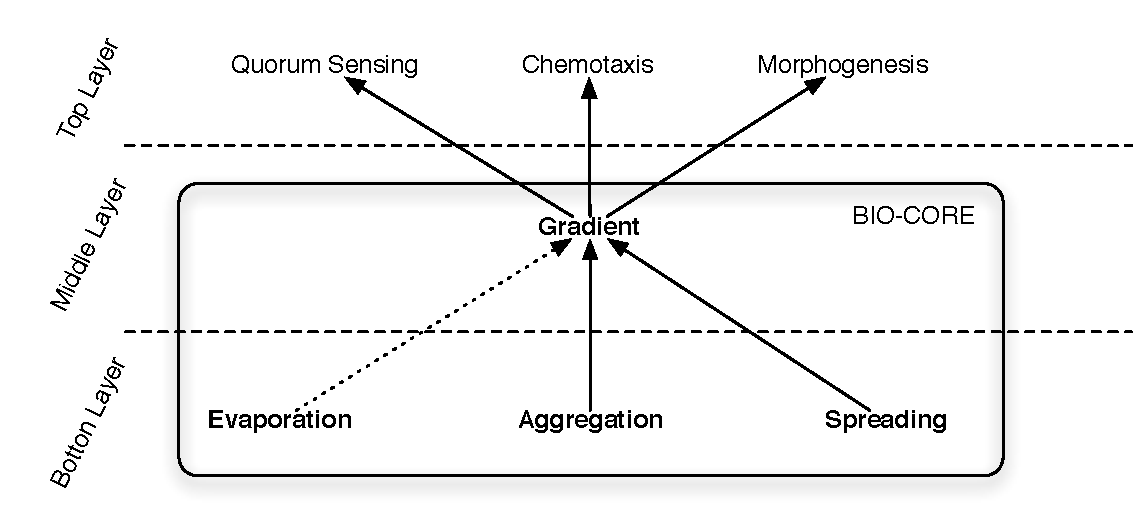
\includegraphics[width=\textwidth]{img/sc-basic-mech.pdf}
\end{center}
\caption{Self-organising patterns and their relationships}
\label{fig:patterns} 
\end{figure}

Several recent works (\cite{FDMVA-NACO2012,GVO-CEEMAS2007,Mam06,Wolf2007}) have focussed on the issue of making self-organisation mechanisms systematically applicable, by proposing descriptions of those mechanisms under the form of catalogues of software design patterns~\cite{Gamma1995}.
%
Recent studies on self-organisation identified existing and new patterns to design computing applications featuring desirable properties of adaptation and robustness to unpredicted changes in the environment, such as human interaction, network mobility and faults, events in the physical environment.
%
As a reference, we consider the work in \cite{FDMVA-NACO2012}, in which a catalogue of patterns for self-organisation is introduced.
%
Following a series of work in self-organising coordination \cite{VCMZ-TAAS2011,sapereecolaws-sac2012}, such a catalogue uses a paradigm of chemical-like transformation rules (manipulating information items residing in the network nodes) to specify pattern behaviour and pattern combination.
%
This catalogue is organised in layers (see \Cref{fig:patterns}): low-level patterns achieve basic self-organisation mechanisms (Spreading, Aggregation and Evaporation), middle-level patterns are used to spatially organise information (gradient), and high-level patterns exploit such information to achieve individual or social goals in a multi-agent system (quorum sensing, chemotaxis, morphogenesis).

\subsection{Gradient}
\label{gradient}
A simple though paramount data structure that is a building block of many of the more advanced patterns is the spatial gradient, which assigns to each node a value $\varGamma$ depending on its position in time and space and on its context \cite{mamei2009acm,crf,VCMZ-TAAS2011}.
%
This structure originates in one or more devices called sources.
%
In every source device, $\varGamma=0$.
%
In every other device, let $N$ be the set of devices connected with it, and let $n$ be the n-th neighbouring device.
%
For this device, $\varGamma=[\min(f(n)) | n \in N]$: namely, the value of the device is the minimum of a function which operates on the neighbours.
%
For instance, if $ \forall n \colon f(n)=\varGamma_{n}+1$, where $\varGamma_{n}$ is the value of the gradient in $n$, then the local value will reflect the minimum hop count towards the nearest source.
%
If $f(n) = \varGamma_{n} +d(n)$ where $d(n)$ measures the actual distance from the device towards $n$, then the value of the gradient will approximate the distance from the nearest source.
%
Finally, along with the local value, a gradient can carry more information, e.g. some strings, the position of $n$, or numeric values.
%
In this case, the gradient is a ``gradcast'', namely a mean to transmit an keep an information up-to date in both space and time.
%
This can be understood as a computational field \cite{SpatialIGI2013,mamei2009acm,VCMZ-TAAS2011}, namely, a distributed data structure mapping each node of the network (or of a subpart of the network) to some (possibly structured) value.

Interestingly, the Gradient pattern can be designed to automatically self-heal to changes in the topology and to movement of the source \cite{flexiblegradients}.
%
% TODO problems with gradient salita lenta
\cite{crf}

\subsection{Chemotaxis}

As a main example of upper-level pattern exploiting gradient, chemotaxis is about making a mobile agent (or some information) descending a gradient data structure so as to reach the source from any node the Gradient structure has reached.
%
This is achieved by making the agent continuously reading the estimated distance value as reported in the gradient annotations stored in its neighbourhood, and then moving towards the node exposing minimum distance -- the source is eventually reached by construction.
%
This pattern finds applications in long distance communications, or in physical items retrieval in situated applications such as those of pervasive computing.

\section{Tuple-based coordination}

In a tuple-based coordination model \cite{coordbook2001--ch04}, software agents synchronize, co-operate, and compete based on \emph{tuples}, which are simple data structures representing information chunks.
%
Tuples are made available in \emph{tuple spaces}, which are shared information spaces working as the \emph{coordination medium}.
%
Coordination occurs by accessing, consuming, and producing tuples in an \emph{associative} way, relying on the actual content of tuples and not on any form of naming, addressing, or indexing.
%
An interesting survey of the technologies and platforms \cite{adaptivenesslinda-esoaI} analyses the suitability of tuple-based coordination systems in supporting openness, unpredictable changes in distributed environments, and several aspects related to adaptiveness: requirements that are of primary importance in pervasive systems.

Several implementations from both academia and industry exist.

\begin{description}
 \item[Anthill] \cite{anthill} is a framework meant to support design and development of adaptive peer-to-peer applications, in which each node is provided with a local tuple space, agents can travel the network and interact indirectly reading, writing and retrieving tuples.

 \item[Biochemical tuple spaces] \cite{biochemicalTupleSpaces} is a framework in which a tuple resembles a chemical substance, a notion of activity/pertinency value for tuples is used to model chemical concentration, coordination rules are structured as chemical reactions evolving tuple concentration over time, a tuple space resembles a single-compartment solution, and finally a network of tuple spaces resembles a tissue-like biological system.

 \item[\cartago{}] \cite{RPV-JAAMAS2011} is a general purpose framework/infrastructure that makes it possible to program and execute virtual environments - also said virtual / application / software environments - for multi-agent systems.

 \item[GigaSpaces XAP]\footnote{\url{http://www.gigaspaces.com}} (pronounced zap) is a scale-out application server.

 \item[JavaSpaces] \cite{javaspaces1999,javaspaces} are best considered as distributed shared memory with additional features which provide transactional integrity and support for the handling of failure. They are best suited to problems which can be modelled as flows of objects.

 \item[Lime] \cite{murphy2006lime} is a coordination model and middleware based on the ideas found in Linda, a shared tuple space model developed at Yale in the 1980s. Lime has three primary incarnations, each tailored for a specific environment, ranging from mobile ad hoc networks to sensor networks with base stations or with actuators.

 \item[Linda] \cite{linda-toplas7} is the common ancestor of every tuple based coordination framework.

 \item[MARS] \cite{mars} implements a coordination architecture based on Linda-like tuple spaces, associated to each execution environment, where agents can store and retrieve messages in a spatial and temporal uncoupled way.
 %
 In addition, MARS is programmable, i.e., agents can associate reactions to the operations made on the space.

 \item[Molecules of knowledge] \cite{mariani2013molecules} (MoK for short) is a model for knowledge self-organisation, exploiting the biochemical metaphor for its basic abstractions, and biochemical coordination as its coordination model.
 %
 As far as the basic MoK abstractions are concerned, in MoK knowledge atoms are generated by knowledge sources in shared spaces -- compartments -- self-aggregate to shape knowledge molecules, and autonomously move toward knowledge consumers, whose actions (either epistemic or not) are represented as enzymes.
 %
 As far as the MoK computational model is concerned, MoK features biochemical tuple spaces for the creation, aggregation, diffusion and consumption of knowledge atoms and molecules.

 \item[SwarmLinda] \cite{swarmlinda} is a middleware that exploits the idea of the collective intelligence, displayed by swarms of ants, for guiding agents in charge of tuple storage and efficient tuple retrieval. Tuples are handled as sort of pheromones or items that ants (agents) relocate in order to improve overall efficiency.

 \item[T Spaces] \cite{tspaces-ibmsj37} is a tuplespace-based network communication buffer with database capabilities that enables communication between applications and devices in a network of heterogeneous computers and operating systems.

 \item[TOTA] \cite{mamei2009acm, tota2} is a tuple-based middleware explicitly conceived to support field-based coordination for adaptive context-aware and spatially-aware activities in pervasive computing scenarios.
 %
 In TOTA, each tuple also carries with it a diffusion rule and a maintenance rule in addition to a content. Tota inspired other works, such as the evolving tuples model \cite{evolvingtuples}, which adds to the tuples a form of context awareness, in form of possible evolution and adaptation to environmental changes.

 \item[TuCSoN] \cite{tucson-aamas99} is a Java library providing coordination as a service to Java and tuProlog agents.
 %
 TuCSoN is a model for the coordination of distributed processes, as well as autonomous, intelligent and mobile agents.
 %
 TuCSoN exploits tuple centres as its coordination media, which are tuple spaces enhanced with the notion of behaviour specification, thanks to the ReSpecT language.
\end{description}

\subsection{SAPERE}
SAPERE\footnote{The model was developed as part of an EU-funded research project. See \url{http://www.sapere-project.eu/}.} \cite{sapere-procedia7} is a nature-inspired coordination model and framework to support the design and development of composite pervasive service systems.
\begin{figure}
\centering
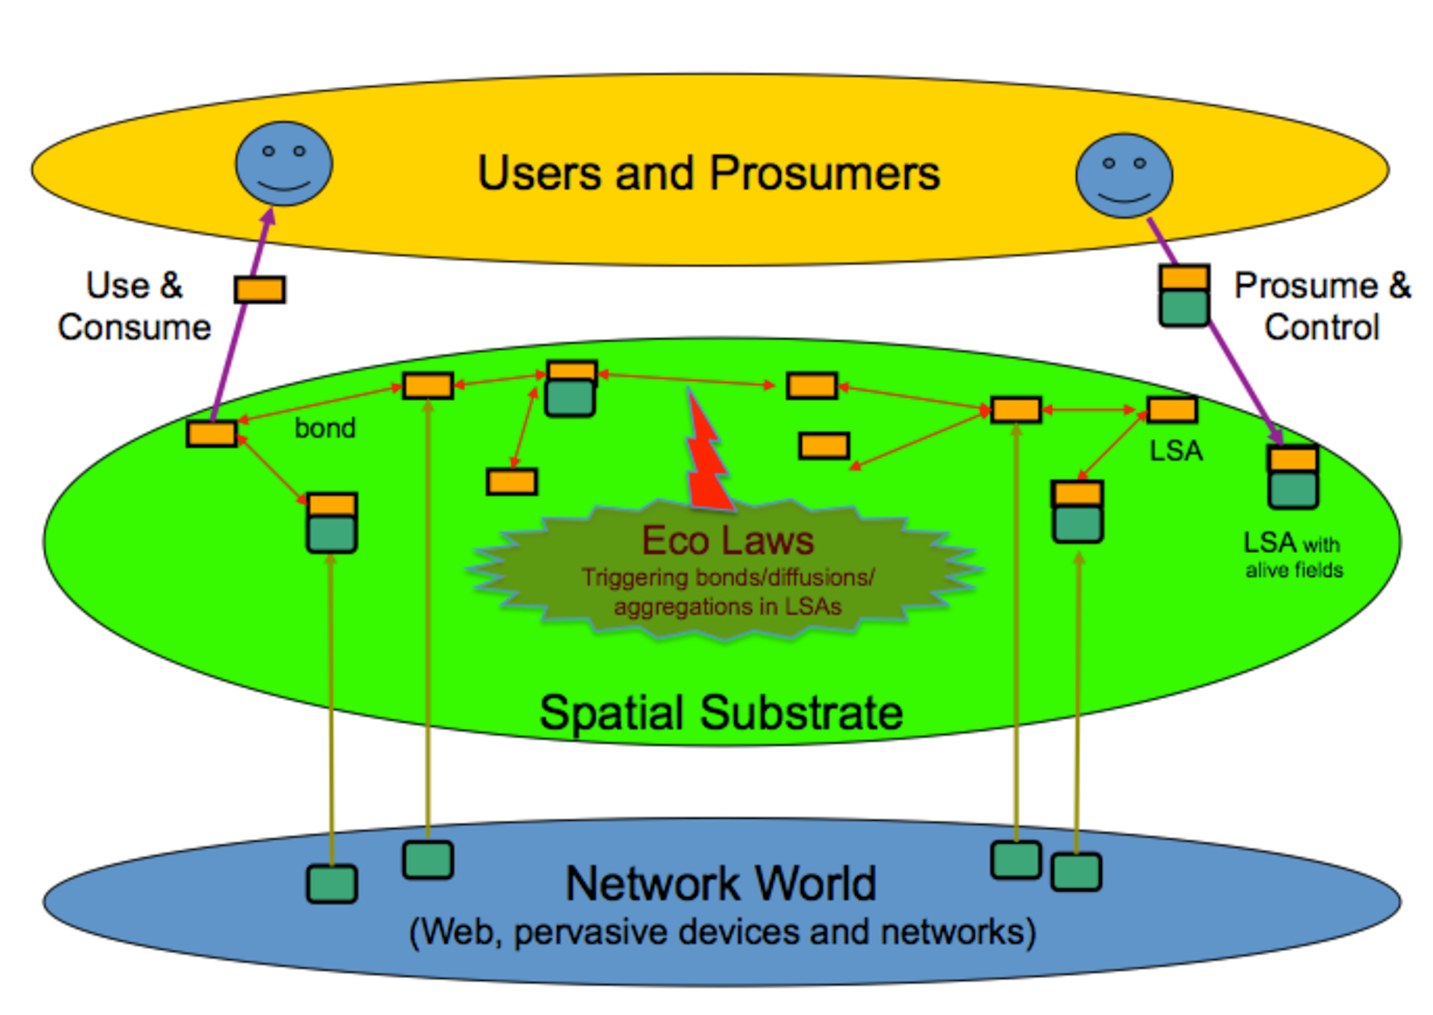
\includegraphics[width=0.8\textwidth]{img/architecture_2.pdf}
\caption[SAPERE reference architecture]{The SAPERE reference architecture.}
\label{img:sapere-architecture}
\end{figure}
%
Its reference architecture and coordination model synthesize from existing nature-inspired approaches, such as \cite{biochemicalTupleSpaces, frameworkSelfOrg, VCMZ-TAAS2011, wordNet}, and is based on an assumption of spatial, local interactions (to be realized via a network of distributed tuple spaces), which is in line with all nature-inspired approaches.
%
Its coordination laws make it possible to express and deploy general nature-inspired distributed algorithms and coordination patterns.
%
SAPERE abstracts a pervasive environment as a non-layered \emph{spatial substrate} deployed upon a dense network of connected heterogeneous ICT devices (\Cref{img:sapere-architecture}).
%
SAPERE acts as a shared coordination medium embodying the basic laws of coordination.
%
Its core components are \cite{sapereecolaws-sac2012}:
\begin{description}
 \item[LSA] Because of the need to tolerate diversity, a cornerstone of pervasive ecosystems is that a uniform representation is required for the various software agents living within them (whether they run on smartphones, sensors, actuators, displays, or any other computational device).
 %
 Such a representation needs to expose any information about the agent (state, interface, goal, knowledge) that is pertinent for the ecosystem as a whole or for any subpart of it.
 %
 In SAPERE this description is called ``Live Semantic Annotation'' for it should continuously represent the state of its associated component (live), and it should be implicitly or explicitly connected to the context in which such information is produced, interpreted and manipulated (semantic)—possibly relying on standard technologies and techniques of the Semantic Web, like RDF \cite{manola2004primer}.
 %
 \item[LSA-space] To handle situatedness, the behaviour of each agent strictly depends on the local context in which it runs, that is, on the state of other agents living in the same locality (intended as network neighbourhood).
 %
 As such, the LSAs of each agent are reified in a distributed space (called an “LSA-space”) acting as the fabric of the ecosystem, where “context” is simply defined and represented as the set of LSAs stored in a given locality.
 %
 \item[LSA bonding] Additionally, and in order to make any agent act in a meaningful way with respect to the context in which it is situated, special mechanisms are needed to provide a fine-tuned control of what to each agent is visible/modifiable and what is not.
 %
 SAPERE tackles this issue by allowing an LSA to include bonds (i.e., references) to other LSAs in the same context.
 %
 It is only via a bond that an agent can inspect the state/interface of another agent and act accordingly, while modifications are allowed only to the LSAs an agent injected itself.
 %
 \item[Eco-laws] Because of adaptivity, while agents enact their individual behaviour by observing their context and updating their LSAs, global behaviour (i.e., global system coordination) is enacted by self-organising manipulation rules of the LSA-space, called eco-laws.
 %
 They can execute deletion/update/movement/re-bonding actions applied to a small set of LSAs in the same locality.
 %
 SAPERE structures such eco-laws as chemical-resembling reactions over LSAs—similarly to other approaches like \cite{BanP09,biochemicalTupleSpaces,VCMZ-TAAS2011}.
\end{description}

\section{Aggregate programming}

\begin{figure}
\centering
\subfigure[Continuous Space]{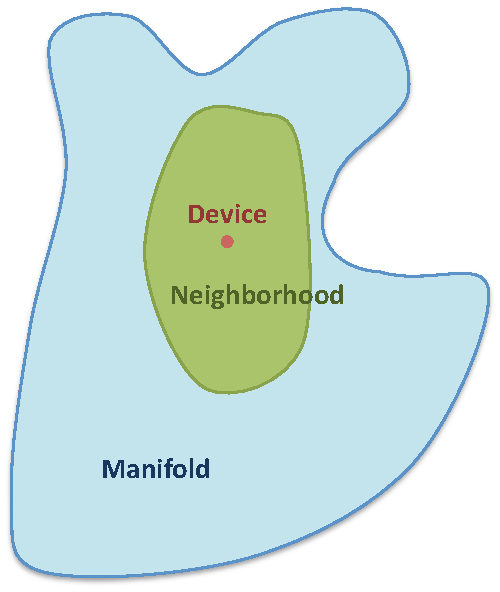
\includegraphics[width=0.4\columnwidth]{img/space-continuous}\label{img:medium}}
\hspace{0.01\columnwidth}
\subfigure[Discrete Network]{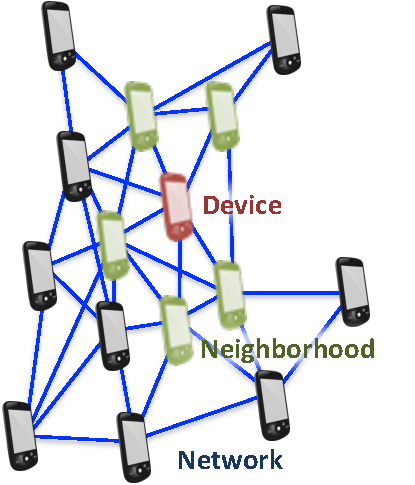
\includegraphics[width=0.4\columnwidth]{img/space-discrete}\label{img:mediumnet}}
\caption[Discrete approximation of continuous]{Computational field models originate from approximation of continuous space (a) with discrete networks of devices (b).}
\label{img:space}
\end{figure}

Aggregate programming is founded on the observation that in many cases the users of a system are much less concerned with individual devices than with the services provided by the collection of devices as a whole.
%
Typical device-centric programming languages, however, force a programmer to focus on individual devices and their interactions.
%
As a consequence, several different aspects of a distributed system typically end up entangled together: effectiveness and reliability of communications, coordination in face of changes and failures, and composition of behaviours across different devices and regions.
%
This makes it very difficult to effectively design, debug, maintain, and compose complex distributed applications.

Aggregate programming generally attempts to address this problem by providing composable abstractions separating these aspects:
\begin{enumerate}
 \item device-to-device communication is typically made entirely implicit, with higher-level abstractions for controlling efficiency/robustness trade-offs;
 \item distributed coordination methods are encapsulated as aggregate-level operations (e.g., measuring distance from a region, spreading a value by gossip, sampling a collection of sensors at a certain resolution in space and time); and
 \item the overall system is specified by composing aggregate-level operations, and this specification is then transformed into a complete distributed implementation by a suitable mapping.
\end{enumerate}

In short, the key idea behind aggregate programming is to provide languages and APIs that allow a distributed collection of devices to be programmed in terms of their collective behaviours, keeping outside the sight of the software designer details on how such coordination is actually implemented.

A large number of very diverse aggregate programming approaches have been proposed, including abstract graph processing (e.g.,~\cite{kairos}), declarative logic (e.g.,~\cite{Meld}), map-reduce (e.g.,~\cite{dean2008mapreduce}), streaming databases (e.g.,~\cite{tinydb}), and knowledge-based ensembles (e.g.,~\cite{SCEL})---for a detailed review, see~\cite{SpatialIGI2013}.

Despite the fact that all of them are based on viewing the collection of devices as an approximation of continuous space (as depicted in \Cref{img:space}), most aggregate programming approaches, however, have been too specialized for particular assumptions or applications to be able to address the complex challenges of these emerging environments.

\subsection{Proto}
\label{proto}

Proto is a language and middleware~\cite{proto} that exploits field-based coordination to orchestrate the activities of sensor-actuator networks in a aggregate way.
%
Proto is based on the notion of a {\em computational field}---a map from devices comprising the system to (possibly structured) values, which is treated as unifying first-class abstraction to model system evolution and environment dynamics.

The programming constructs are combined together to form programs, whose semantics is defined in terms of a sequence of synchronous rounds of evaluation by a discrete network of devices called ``computational rounds''.
%
In practice, however, there is no requirement for synchrony, and each device can evaluate its own computational rounds independently.

Despite its qualities, Proto still lacks many features expected in a modern programming language and has an implementation encumbered by a number of obsolete considerations that make it difficult to maintain and extend.
%
Moreover, Proto has a complex operational semantics, that makes it hard to develop mathematical proofs about Proto programs.
%
Such complexity is one of the pillars sustaining the efforts behind Field Calculus (see \Cref{field-calculus}).

\subsection{Field Calculus}
\label{field-calculus}

Field Calculus is an attempt to find a unifying model for programming \emph{computational fields} as a generalization of a wide range of existing approaches.
%
It is a fragment of Proto, (see \Cref{proto}), but it also takes inspiration from \cite{mamei2009acm,regiment,VCMZ-TAAS2011,tota2,nagpalphd,yamins,regiment}.
%
Formalized as the computational field calculus~\cite{VDB-FOCLASA-CIC2013}, this universal language appears to provide a theoretical foundation on which effective general aggregate programming platforms can be built.

Critically, although originally derived from continuous-space concepts, the calculus does not depend on them and is applicable to any network.
. %
Field calculus is expressive enough to be a universal computing model~\cite{BVD-SCW14} but terse enough to enable a provable mapping from aggregate specifications to equivalent local implementations.

Field calculus~\cite{VDB-FOCLASA-CIC2013} hence provides a key theoretical and methodological foundation for aggregate programming.
%
Its aim is to provide a universal model that is suitable for mathematical proofs of general properties about aggregate programming and the aggregate/local relationship, just as $\lambda$-calculus~\cite{LambdaCalculus} provides for functional programming, $\pi$-calculus for parallel programming~\cite{PiCalculus}, or Featherweight Java~\cite{FJ} for Java-like object-oriented programming.

In the field calculus, everything is a field: computational fields are used to model every aspect of distributed computation, including input from sensors, network structure, environment interactions, distributed computations (e.g. progressive aggregation and spreading processes), and output for actuators.
%
In particular, field calculus is constructed using five basic constructs:
\begin{enumerate}
 \item function definition and evaluation;
 \item ``built-in'' operations for stateless local computation, e.g.,
addition, multiplication, reading a sensor;
 \item a time-evolution construct which allows for stateful computation;
 \item a neighbour-value construct that creates a field of values from a device's neighbours;
 \item a restriction operator to select which computations to perform in various regions of space and time.
\end{enumerate}

As well as in Proto, in Field Calculus the semantics of programs created by combining such constructs is defined in terms of a sequence of (possibly synchronous) ``computational rounds''.

The minimal syntax of field calculus has allowed its semantics, including proper coherence of device interactions, to be proven correct and consistent~\cite{VDB-FOCLASA-CIC2013}.
%
Additionally, despite its definition in terms of discrete semantics, field calculus is also space-time universal~\cite{BVD-SCW14}, meaning that it can approximate any field computation, either discrete or continuous, with arbitrary precision given a dense enough network of devices.

This, then, is the key contribution of field calculus: any coordination method with a coherent aggregate-level interpretation is guaranteed to be expressible in field calculus.
%
Such a method can then be abstracted into a new aggregate-level operation, which can be composed with any other aggregate operation using the rules of built-in functions over fields.
%
Moreover, it can have its space-time extent modulated and controlled by restriction, all while guaranteed that the relationship between global specification and local implementation will always be maintained.

\begin{figure}
\centering
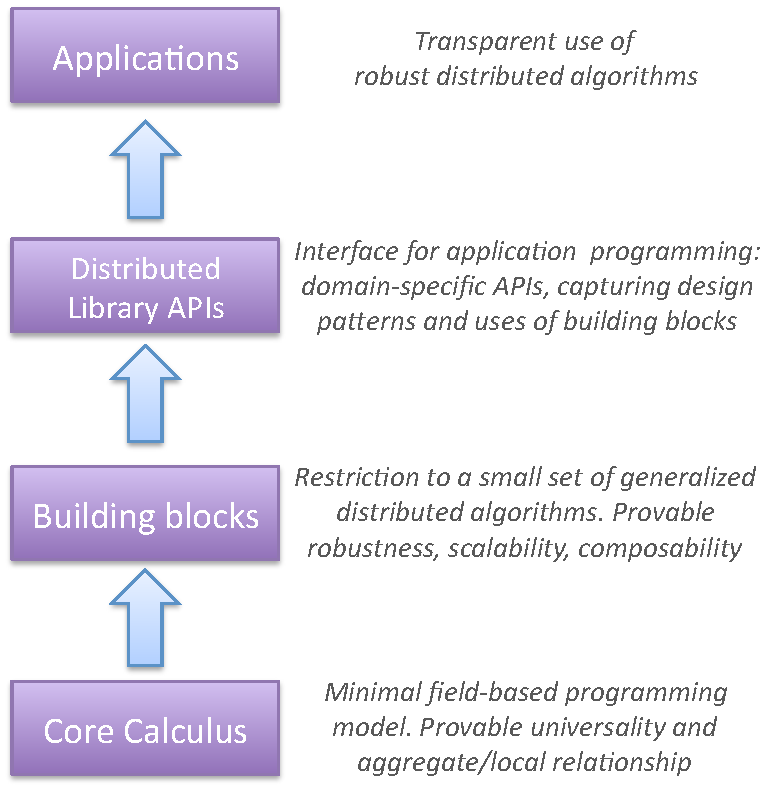
\includegraphics[width=0.99\textwidth]{img/aggregate-tower}
\caption[Layered approach]{Layered approach for development of spatially-distributed systems via aggregate programming.}
\label{img:researchprogram}
\end{figure}

Such a core calculus, like any other, is more a theoretical framework than a practical programming language.
%
In practice, in fact, effective aggregate programming for real-world distributed applications is likely to require a layered approach such as the one depicted in \Cref{img:researchprogram}, of which field calculus represents the first block.
%
Some of the prior approaches on which field calculus is based provide very similar semantics (most notably Proto), but they all suffer from some combination of design and implementation problems that render them impractical for widespread adoption.
%
Besides Proto, which is probably the closest to a practical programming environment and whose problems have already been described in \Cref{proto}, others, such as \cite{VPB-COORD2012}, have only minimal implementation.

\subsubsection{Basics and Syntax}

The basic mechanisms behind Field Calculus can be studied through its the syntax, reported in Figure \ref{fig:source:syntax}.
%
We take the global, aggregate-level viewpoint, considering the main syntactic element $\e$ as being a field expression, or simply a field.
%
As a standard syntactic notation in calculi for object-oriented and functional languages \cite{FJ}, the overbar notation denotes metavariables over lists, e.g., $\overline \e$ ranges over lists
of expressions, written $\e_1\;\e_2\;\ldots\;\e_n$.

A basic expression can be a literal value $\lvalue$ (also called local value), such as a floating point number, a boolean, or a tuple---note most of the ideas of computational fields are agnostic to the
structure of such values.
%
According to the global viewpoint, a literal field expression $\lvalue$ actually represents the constant function mapping $\lvalue$ to all nodes.
%
A basic expression can also be a variable $\xname$, which can be the formal parameter of a function or a store of information to support stateful computations (see $\repN$ construct below).

\begin{figure}[!t]{
\centerline{\framebox[\textwidth]{$
\begin{array}{@{\hspace{-0.1cm}}lcl@{\hspace{0.5cm}}r}
 \e & \BNFcce &  \xname \;
    \; \BNFmid \; \lvalue
    \; \BNFmid \; (\oname \; \overline{\e})
    \; \BNFmid \; (\fname \; \overline{\e})
    \;\BNFmid \; (\repN \; \xname\; \we \; \e)
    \; \BNFmid \; (\nbrN \; \e)
    \; \BNFmid \; (\ifN \; \e\; \e \; \e)
    &   {\footnotesize \mbox{expression}} \\
 \we & \BNFcce &  \xname \;
    \; \BNFmid \; \lvalue                                                              &   {\footnotesize \mbox{variable or value}} \\
     \FCFUNCTION & \BNFcce & (\defK \; \fname (\overline{\xname}) \; \e)
  &   {\footnotesize \mbox{function}}\\
    \PROGRAM & \BNFcce & \overline{\FCFUNCTION}  \; \e
  &   {\footnotesize \mbox{program}}     \\
 \end{array}
 $}}}
\caption{Surface syntax of Field Calculus, from \cite{VDB-FOCLASA-CIC2013}}
\label{fig:source:syntax}
\end{figure}

Such basic expressions (values and variables) can be composed by the following 5 constructs.

The first one is \emph{functional composition}, a natural means of manipulating fields as they are functions themselves: $(\oname \; \e_1 \e_2\;\ldots\;\e_n)$ is the field obtained by composing together all the fields $\e_1,\;\e_2,\;\ldots,\;\e_n$ by an operator $\oname$.
%
Operators are built-in, and include standard mathematical ones (e.g. addition, sine): they are applied in a pointwise manner to all devices.
%
For instance, if $\e_t$ is a field of Fahrenheit temperatures, then the corresponding field of Celsius temperatures is naturally written \mbox{\texttt{(* (/ 5 9) (- $\e_t$ 32))}}.
%
Execution of built-in operators is context-dependent, i.e., it can be affected by the current state of the external world.
%
So, 0-ary operator $\self$ gives a field that maps each device to its identifier, \texttt{dt} maps each device to the time elapsed since its previous computation round, and finally \texttt{nbr-range} maps each device to a table associating estimated distances to each neighbour (such a table being a field itself).

The second construct is \emph{function (definition and) call}, which is used as abstraction tool and to support recursion: $(\fname \; \e_1\;\e_2\;\ldots\;\e_n)$ is the field obtained as result of applying user-defined function $\fname$ to the fields $\e_1,\;\e_2,\;\ldots\;\e_n$. Such functions are declared with syntax $(\defK \; \fname (\overline{\xname}) \; \e)$.
%
For instance, after definition $\texttt{(\defK~convert (x) (* (/ 5 9) (- x 32)))}$, expression \texttt{(convert $\e_t$)} denotes the same field of Celsius temperatures as above.
%
Note that function definitions, along with the top-level expression, form a program $\PROGRAM$.

The third construct is \emph{time evolution}, used to keep track of a changing state over time: $(\repN \; \xname\; \we \; \e)$ is initially the field $\we$ (a local value or a variable) that is stored in the new variable $\xname$, and at each step in time is updated to a new field as computed by $\e$, based on the prior value of $\xname$.
%
For instance, \mbox{\texttt{(\repN~x 0 (+ x 1))}} is the (evolving) field counting in each device how many rounds that device has computed.
%
Similarly, \mbox{\texttt{(\repN~x 0 (+ x (dt)))}} is the field of time passing.

The fourth construct is \emph{neighbourhood field construction}, the mechanism by which information moves between devices: $(\nbrN \; \e)$ maps each device to the field of its neighbours' local value of field $\e$; hence, it is a field of neighbourhood fields like the output of \texttt{nbr-range} above. As an example, let \texttt{min-hood} be the operator taking a neighbourhood field and returning its minimum value, then \texttt{(min-hood (nbr $\e_t$))} is the field mapping each device to the minimum temperature perceived in its neighbourhood.

The last construct is \emph{domain restriction}, a sort of distributed branch: $(\ifN \; \e_0\; \e_1 \; \e_2)$ is the field obtained by superimposing field $\e_1$ computed everywhere $\e_0$ is true and $\e_2$ everywhere $\e_0$ is false.
%
As an example \mbox{\texttt{(if $\e_{\mathit{fah}}$ $\e_t$ (convert $\e_t$))}} is the field of temperatures provided in Fahrenheit (resp. Celsius) where the field $\e_{\mathit{fah}}$ is true (resp. false).
%
Restriction is the most subtle of the five mechanisms, because it has the effect of preventing the unexpected spreading of computation to devices outside of the required domain, even within arbitrarily nested function calls, as will be clarified in the following.

Here are some examples to illustrate how these five key mechanisms can be combined to implement useful spatial patterns.
%
\begin{samepage}
\begin{Verbatim}[
                  frame=single,
                  %baselinestretch=,
                  commandchars=\\\{\}]
(\km{def} \fn{gossip-min} (source) (\km{rep} d source (\pr{min-hood} (\km{nbr} d))))

(\km{def} \fn{distance-to} (source)
  (\km{rep} d infinity (\pr{mux} source
     0
     (\pr{min-hood} (\pr{+} (\km{nbr} d) (\pr{nbr-range})))
     )))

(\km{def} \fn{distance-obs-to} (source obstacle)
      (\km{if} (\pr{not} obstacle) (\fn{distance-to} source) infinity))
\end{Verbatim}
\end{samepage}
%
Function {\tt gossip-min} takes a {\tt source} field and produces a new field mapping each device to the minimum value that {\tt source} initially takes.
%
The {\tt rep} construct initially sets the output variable {\tt d} at {\tt source}, and it iteratively updates the value at each device with the minimum one available in {\tt d}'s neighbours.
%
Hence, {\tt gossip-min} describes a process of gossiping values until the minimum one converges throughout the network.

Similarly, function {\tt distance-to} takes as its input a {\tt source} field holding boolean values, and returns a new scalar field that maps each device to the estimated distance to the nearest device where {\tt source} is true.
%
This works by first setting {\tt d} to infinity, then updating it as follows: sources are of course at distance $0$, while all other devices use the triangle inequality, finding the minimum sum of a neighbour's estimated distance {\tt d} and the distance to that neighbour.
%
Operator \texttt{mux}, used to combine the two, is a purely functional multiplexer, which uses the first input to choose whether to return the second or third.
%
The field returned by {\tt distance-to} is a \emph{gradient}.

The last definition exemplifies the use of construct \ifK{}. It creates two different spatial domains: one where the obstacle is present (field {\tt obstacle} holds positive boolean value) and one where is not. In the former an infinity constant field is computed; in the latter we spread the {\tt distance-to} field.
%
As a result, distance estimation as provided by {\tt distance-to} automatically takes into account the need of circumventing obstacle areas, since information does not cross the two domains due to the semantics of \texttt{\nbrN}.

\subsubsection{Semantics}

The computational field calculus formalisation is set forth in \Cref{fig:calculus}.
%
For a complete description of the symbols and their meaning, the interested reader should refer to \cite{VDB-FOCLASA-CIC2013}.

The most important point for the discussion of this thesis is the compactness of such core semantics: it can be summarised in a single page of rules, while several pages would be required to host the complete semantics of Proto, the language from which Field Calculus is derived.
%
The number of pages required to host a formal semantics is clearly a rule of thumb, but gives also the less experienced reader some idea on how intricate is Proto with respect to Field Calculus.
%
A more lightweight semantics has two key advantages:
\begin{enumerate}
 \item many properties become mathematically treatable and can be and proved;
 \item provides a solid guideline for practical languages to be designed and implemented.
\end{enumerate}
%
The first point is very relevant for this thesis, since a solid mathematical background is the best possible foundation for a reliable engineering procedure.
%
The second point will be exploited in \Cref{protelis-language}, where a new practical language building on Field Calculus will be presented.
%
Such language's interpreter adheres to the operational semantics defined in \Cref{fig:calculus}, and consequently shares all the nice properties of field calculus demonstrated in \cite{VDB-FOCLASA-CIC2013}.

%
% $\sigma$ ranges over device unique identifiers and $\fvalue$ over field values (mapping set of devices to local values).
% %
% Given any meta-variable $y$, $\option{y}$ ranges over an element $y$ or the \emph{null decoration} (which in the calculus is $\circ$ when it has to be expressed, and blank otherwise).
% %
% The calculus is agnostic to the syntax of local values: it is only assumed that they include at least device identifiers and value $0$.
% %
% Metavariables \fclfalse{} and \fcltrue{} range over boolean-interpreted values, orderly $0$ and any other value.

\begin{figure}{
 \framebox[1.015\columnwidth]{$
\begin{array}{l}
%%%  SYNTAX
\textbf{\hspace{-3pt}Runtime Expression Syntax:}\\
\begin{array}{@{\hspace{-0.0cm}}lcl@{\hspace{0.5cm}}r}
%
\lre & \BNFcce &  \labelled{\re}{\orv} &   {\footnotesize \mbox{runtime expression (rte)}} \\
%
 \re & \BNFcce &  \xname
    \, \BNFmid \, \rv
    \, \BNFmid \, (\labelledC{\nbrN}{} \, \lre) \, \BNFmid \, (\labelledC{\ifN}{} \, \lre\, \lre \, \lre)  \,\BNFmid \, (\labelledC{\repN}{\asuper} \, \xname\, \we \, \lre)  \, \BNFmid \, (\labelledC{\fname}{\asuper} \, \overline{\lre})
     \, \BNFmid \, (\oname \, \overline{\lre}) &   {\footnotesize \mbox{auxiliary rte}} \\
%
\rv & \BNFcce &  \lvalue  \, \BNFmid \, \phi &   {\footnotesize \mbox{runtime value}} \\
%
\asuper & \BNFcce & \option{\re} &  {\footnotesize \mbox{superscript}}\\
%
\we & \BNFcce &  \xname  \, \BNFmid \, \lvalue  &   {\footnotesize \mbox{variable or local value}} \\
%
\phi & \BNFcce &  \fvalues{\overline\sigma}{\overline\lvalue} &   {\footnotesize \mbox{field value}} \\
%
\Trees & \BNFcce &  \treeslot{\overline\sigma}{\overline\lre} &   {\footnotesize \mbox{tree environment}} \\
%
\Env & \BNFcce &  \memslot{\overline\xname}{\overline\rv} &   {\footnotesize \mbox{variable environment}} \\[5pt]
%
\end{array}\\
\hline\\[-8pt]
%%%  CONGUENCE CONTEXTS
%
\begin{array}{lcl}
 \multicolumn{3}{l}{\hspace{-3pt}\textbf{Congruence Contexts:}}\\
 \ctx & \BNFcce & (\labelledC{\nbrN}{} \; \hole)
        \; \BNFmid \;  (\fname^{\asuper} \; \overline{\lre} \; \hole \; \overline{\lre})
        \; \BNFmid \;  (\oname \; \overline{\lre} \; \hole \; \overline{\lre})
        \; \BNFmid \; (\ifN^{} \; \hole \; {\lre} \; {\lre})
        \; \BNFmid \; (\ifN^{} \; \labelled{\re}{\fcltrue{}} \; \hole \; \lre)
        \; \BNFmid \; (\ifN^{} \; \labelled{\re{}}{\fclfalse{}} \; \lre{}  \; \hole \;)
        %&   {\footnotesize \mbox{congruence context}}\\
    % & {\footnotesize \mbox{evaluation context}} \\
    \end{array}\\
\hline\\[-8pt]
%%%  ALIGNMENT CONTEXTS
%
\begin{array}{lcl}
 \multicolumn{3}{l}{\hspace{-3pt}\textbf{Alignment contexts:}}\\
 \actx & \BNFcce & \ctx \;\BNFmid \; (\labelledC{\repN}{\asuper} \; \xname\; \we\; \hole )
        %\; \BNFmid \;  (\labelledC{\fname}{\re} \; \overline{\lre} \; \hole \; \overline{\lre})
         \; \BNFmid \;  (\labelledC{\fname}{\hole} \; \labelled{\overline{\re}}{\overline{\rv}})
        %& {\footnotesize \mbox{aligment context}}\\
    % & {\footnotesize \mbox{evaluation context}} \\
    \end{array}\\
\hline\\[-8pt]
%
%%%  OPERATORS
%
%\begin{array}{c@{\hspace{35pt}}c}
%
%\multicolumn{2}{l}{\hspace{-5pt}\textbf{Operators:}}\\[5pt]
%\begin{array}{l@{\hspace{10pt}}l}
%\phi,\phi' & \textrm{disjoint union of maps}\\
%\textit{args}(\fname) & \textrm{arguments of $\fname$}\\
%\textit{body}(\fname) & \textrm{body of $\fname$}\\
%\end{array}
%&
%\begin{array}{l@{\hspace{10pt}}l}
%\textit{dom}(\phi) & \textrm{map dominium}\\
%\erase{\lre} & \textrm{erase $\lre$ to \texttt{e}}\\
%\textit{exec} & \textrm{built-in evaluator}\\
%\end{array}
%
%\end{array}\\[5pt]
%
%
%
%\hline\\[-8pt]
%
%%%  AUXILIARY
%
 \begin{array}{c@{\hspace{20pt}}c}
  \multicolumn{2}{l}{\hspace{-3pt}\textbf{Auxiliary functions:}}\\[4pt]
\begin{array}{rcll}
\inversectx{\actx}{\Trees,\Trees'} & = & \inversectx{\actx}{\Trees},\inversectx{\actx}{\Trees'}\\
\inversectx{\actx}{\treeslot{\sigma}{\labelled{(\actx'[\lre])}{\rv}}} & = & \treeslot{\sigma}{\lre}  \qquad \textrm{if $\actx' \matches \actx$} \\
\inversectx{\actx}{\treeslot{\sigma}{\lre}} & = & \emptyL \qquad \textrm{otherwise} \\[5pt]
\replace{\re}{\asuper} = \re
\\
\replace{\circ}{\asuper} = \asuper
%\multicolumn{2}{c}{\replace{\re}{\asuper} = \re,\;\replace{\circ}{\asuper} = \asuper}
%\multicolumn{4}{c}{\upd{\Env}{\Env'} = \proj{\Env}{\fdom{\Env}\setminus\fdom{\Env'}},\proj{\Env'}{\fdom{\Env'}}}
\end{array}
%
&
%
\begin{scriptsize}
\begin{array}{rcl}
 \\[-0.9cm]
(\labelledC{\nbrN}{} \; \hole) & \matches & (\labelledC{\nbrN}{} \; \hole)\\
(\labelledC{\fname}{\asuper'} \; \lre'_1...\lre'_{i-1} \; \hole \; \lre'_{i+1}...\lre'_n) & \matches & (\labelledC{\fname}{\asuper} \; \lre_1...\lre_{i-1} \; \hole \; \lre_{i+1}...\lre_n)\\
(\oname \; \lre'_1...\lre'_{i-1} \; \hole \; \lre'_{i+1}...\lre'_n) & \matches & (\oname \; \lre_1...\lre_{i-1} \; \hole \; \lre_{i+1}...\lre_n)\\
(\ifN^{} \; \hole \; {\lre'_1} \; {\lre'_2})) & \matches &  (\ifN^{} \; \hole \; {\lre_1} \; {\lre_2}))\\
(\ifN^{} \; \labelled{\re'}{\fcltrue{}} \; \hole \; \lre') & \matches & (\ifN^{} \; \labelled{\re}{\fcltrue{}} \; \hole \; \lre)\\
(\ifN^{} \; \labelled{\re'{}}{\fclfalse{}} \; \lre'  \; \hole \;) & \matches & (\ifN^{} \; \labelled{\re{}}{\fclfalse{}} \; \lre  \; \hole \;)\\
(\labelledC{\repN}{\asuper'} \; \xname\; \we\; \hole ) & \matches &  (\labelledC{\repN}{\asuper} \; \xname\; \we\; \hole )\\
(\labelledC{\fname}{\hole} \;\lre'_1...\lre'_n) & \matches &  (\labelledC{\fname}{\hole} \;\lre_1...\lre_n)
%\multicolumn{2}{c}{\upd{\fvalue}{\fvalue'} = \proj{\fvalue}{\fdom{\fvalue}\setminus\fdom{\fvalue'}},\proj{\fvalue'}{\fdom{\fvalue'}}}\\
%\replace{\re}{\asuper} = \re,\;\replace{\circ}{\asuper} = \asuper & \textrm{replacement}\\
%\textit{args}(\fname) & \textrm{arguments of $\fname$}\\
%\textit{body}(\fname) & \textrm{body of $\fname$}\\
%\erase{\lre} & \textrm{erase $\lre$ to \texttt{e}}\\
%\textit{exec}^\Env & \textrm{built-in evaluator}\\
\end{array}
\end{scriptsize}
%
\end{array}\\[5pt]
%

%
\hline\\[-8pt]
%% OPERATIONAL SEMANTICS
%
\begin{small}
\begin{array}{c@{\;}c}
\multicolumn{2}{l}{\hspace{-3pt}\textbf{Reduction Rules:}}\\[-14pt]
%
&
%
\nulltransition{THEN}{
\opsem{\Trees}{\Env}{
  (\ifN^{} \; \labelled{\re}{\fcltrue{}}\; \labelled{\re'}{\lvalue} \; \lre)
}{
  \labelled{(\ifN^{} \; \labelled{\re}{\fcltrue{}}\; \labelled{\re'}{\lvalue} \; \erase{\lre})}{\lvalue}
}
}
%
\skiptransition
%
\nulltransition{VAL}{ \opsem{\Trees}{\Env}{
  \rv
}{
  \labelled{\rv}{\rv}
} }
%
&
%
\nulltransition{ELSE}{
\opsem{\Trees}{\Env}{
  (\ifN^{} \; \labelled{\re}{\fclfalse{}}\; \lre \; \labelled{\re'}{\lvalue} )
}{
  \labelled{(\ifN^{} \; \labelled{\re}{\fclfalse{}}\; \erase{\lre} \; \labelled{\re'}{\lvalue} )}{\lvalue}
}
}
%
\skiptransition
%
\nulltransition{VAR}{
\opsem{\Trees}{\Env}{\xname}{
  \labelled{\xname}{\proj{\Env(\xname)}{\textit{dom}(\Trees),\oexec(\self)}}}
}
&
 \transition{CONG}{
\opsem{\inversectx{\ctx}{\Trees}}{\Env}{\re}{\lre} }{
\opsem{\Trees}{\Env}{\ctx[\re]}{\ctx[\lre]} }
%
\skiptransition
\transitiontwoprec{NBR}{
\hspace{-20pt}\inversectx{(\labelledC{\nbrN}{} \; \hole)}{\Trees}=\treeslot{\overline\sigma}{\labelled{\overline{\re}}{\overline\lvalue}}
%\hspace{-20pt}\inversectx{(\labelledC{\nbrN}{} \; \hole)}{\Trees}=\treeslot{\overline\sigma}{\labelled{\overline{\re}}{\overline\lvalue}},\treeslot{\overline\sigma'}{\labelled{\overline{\re}'}{\overline\phi}}
}{
\phi=(\treeslot{\overline\sigma}{\overline\lvalue},\fvalues{\oexec(\self)}{\lvalue})
}{
\opsem{\Trees}{\Env}{
  (\nbrN \; \labelled{\re}{\lvalue})
 }{
  \labelled{(\labelledC{\nbrN}{} \; \labelled{\re}{\lvalue})}{\phi}
 }
}
&
\transition{REP}{
\opsem{\inversectx{(\labelledC{\repN}{\option{\lvalue}} \; \xname\; \we\; \hole )}{\Trees}}{
  \Env,(\memslot{\xname}{(\replace{\option{\lvalue}}{\Env(\we)})})}
  {\re}{\labelled{\re'}{\option{\rv}}}
}{
\opsem{\Trees}{\Env}{
  (\labelledC{\repN}{\option{\lvalue}} \; \xname\; \we\; \re )
}{
  \labelled{(\labelledC{\repN}{\replace{\option{\rv}}{\option{\lvalue}}} \; \xname\; \we\; \labelled{\re'}{\option{\rv}} )}{\option{\rv}}
}
}
%
 \skiptransition
\nulltransition{OP}{
\opsem{\Trees}{\Env}{
  (\oname \; \labelled{\overline{\re}}{\overline{\rv}})
}{
  \labelled{(\oname \; \labelled{\overline{\re}}{\overline{\rv}})}{\oexec(\oname,\overline{\rv})}
} } & \transition{FUN}{
\opsem{\inversectx{(\labelledC{\fname}{\hole} \;
\labelled{\overline{\re}\;}{\;\overline{\rv}})}{\Trees}}{(\memslot{\textit{args}(\fname)}{\overline\rv})}{(\replace{\asuper}{\textit{body}(\fname)})}{\labelled{\re}{\option{\rv}}}
}{ \opsem{\Trees}{\Env}{
  (\labelledC{\fname}{\asuper} \; \labelled{\overline{\re}}{\overline{\rv}})
}{
  \labelled{(\labelledC{\fname}{\re} \; \labelled{\overline{\re}}{\overline{\rv}})}{\option{\rv}}
}
}\end{array}
\end{small}
\end{array}$}
}\caption{Device Semantics} \label{fig:calculus}
\end{figure}

% \paragraph{Runtime Expression Syntax}
% 
% A runtime expression is the evaluation tree created out of a surface expression.
% %
% It is similar to expressions in the surface syntax (cf. \Cref{fig:source:syntax}) with the following differences (see \Cref{fig:calculus}):
% \begin{itemize}
%  \item a (runtime) value $\rv$ is either a local value $\lvalue$ or a field value $\fvalue$;
%  \item a run-time expression $\lre$ can be coupled (at any level of depth) with optional \emph{annotation} $\orv$ representing the transient side-effect of a computation;
%  \item constructs \texttt{rep} and function calls can have a \emph{superscript} ($\asuper$) representing the durable side-effect of a computation.
% \end{itemize}
% %
% Note that, syntactically, surface syntax expressions can (and will) be used to denote runtime expressions with null decorations in all annotations and superscripts.
% 
% The erasure operator $\erase{\cdot}$ turns a runtime expression $\lre$ (or an auxiliary rte $\re$) to the surface expression $\erase{\lre}$ (resp.\ $\erase{\re}$) obtained by dropping all annotations and superscripts.
% %
% The erasure of an expression $\lre$ (or $\re$) is defined if and only if for every auxiliary rte $\re'$ occurring in $\lre$ (resp. $\re$): $(i)$ $\re'=(\nbrN\,\labelled{\re''}{\rv})$ implies that the runtime value $\rv$ is a local value, and $(ii)$ $\re'= (\labelledC{\fname}{\re''} \, \overline{\lre})$ implies that $\erase{\re''}$ is the body of the the function $\fname$.
% 
% Note that fields are actually mappings, for which we introduce some syntactic conventions and operators.
% %
% A field value $\fvalue$ can either be written as \mbox{$\fvalues{\sigma_1}{\lvalue_1},\ldots,\fvalues{\sigma_n}{\lvalue_n}$} or be shortened by notation \mbox{$\fvalues{\overline{\sigma}}{\overline{\lvalue}}$}.
% %
% The domain of $\phi$, which is the set $\{\sigma_1,...,\sigma_n\}$, is denoted by $\domof{\phi}$.
% %
% The value $\lvalue_i$ associated to a given device $\sigma_i$ by field $\fvalue$ is retrieved by notation $\fvalue(\sigma_i)$.
% %
% Since a field can be seen as a list, the notation $\emptyL$ is used for the empty field, and comma as list concatenation operator: e.g. $\fvalue,\fvalue'$ is the field having both the mappings of $\fvalue$ and $\fvalue'$.
% %
% We shall sometime restrict the domain of a field $\fvalue$ to a given set of devices $\overline\sigma$, which we denote as $\proj{\fvalue}{\overline\sigma}$.
% %
% When restriction is applied to local values it works as the identity function.
% %
% A tree environment, $\Trees$, maps devices to runtime expressions (namely, it keeps neighbour trees), and a variable environment, $\Env$, maps variables to runtime values.
% %
% Since tree environments and variable environments are also mappings, all the above conventions and operators will be used for them as well.
% 
% To take into account special constants, mathematical operations, usual abstract data types operations, and context-dependent operators, a special function $\oexec$ is introduced.
% %
% This is such that $\oexec(\oname,\overline\rv)$ computes the result of applying built-in operator $\oname$ to values $\overline\rv$.
% %
% In particular, we assume constant \texttt{self} gets evaluated to the current device identifier.
% %
% In order not to escape the domain restricted by operator \ifN, for each primitive operator $\oname$ we assume that: $(i)$ $\oexec(\oname,\rv_1,\cdots,\rv_n)$ is defined (i.e., its evaluation does not get stuck) only if all the field values in $\rv_1,\ldots,\rv_n$ have the same domain; and $(ii)$ if $\oexec(\oname,\rv_1,\cdots,\rv_n)$ returns a field value $\phi$ and there is at least one field value $\rv_i$ in $\rv_1,\ldots,\rv_n$, then $\domof{\phi}=\domof{\rv_i}$.
% 
% \paragraph{Congruence Contexts and Alignment Contexts}
% 
% The operational semantics uses \emph{congruence contexts}, ranged over by $\ctx$, to impose an order of evaluation of subexpressions in an orthogonal way with respect to the actual semantic rules; and it uses \emph{alignment contexts}, ranged over by $\actx$, to  properly navigate into evaluation trees.
% %
% In particular, note that $\ctx$ is a subcase of $\actx$ (see \Cref{fig:calculus}).
% 
% A context $\actx$ is an auxiliary runtime expression with a \emph{hole} $\hole$.
% %
% As usual, we write $\actx[\lre]$ to denote runtime expression obtained by filling the hole  of $\actx$ with the runtime expression $\lre$. If a given runtime expression $\lre$ matches  $\ctx[\lre']$, then $\lre'$ is the next subexpression of $\lre$ where evaluation will occur, positioned in $\lre$ as described by the position of $\hole$ in $\ctx$.
% %
% The way the syntax of congruence contexts $\ctx$ is structured constraints the operational semantics to evaluate the first argument of $\ifN$ and then, depending on its outcome, the second or third, and to non-deterministically evaluate arguments in function and operation calls.
% %
% For instance, the runtime expression \texttt{(* 1$\cdot$1 (+ 2$\cdot$2 3))}  matches $\ctx'[\lre']$ only by $\ctx'=\texttt{(* 1$\cdot$1 $\hole$)}$ and $\lre'=\texttt{(+ 2$\cdot$2 3)}$: this means that $\lre'$ contains the next subexpression to evaluate. The expression $\lre'$, in turn, matches $\ctx''[\lre'']$ only by $\ctx''=\texttt{(+ 2$\cdot$2 $\hole$)}$ and $\lre''=\texttt{3}$. Therefore $3$ is the next subexpression to evaluate (becoming $3\cdot 3$).
% 
% \paragraph{Auxiliary functions}
% 
% The projection operator $\pi$  implements the mechanism for synchronising navigation of an evaluation tree with those of neighbour trees. Namely, $\inversectx{\actx}{\Trees}$ takes a tree environment $\Trees$ and extracts a new tree environment
% obtained by discarding the trees that do not match the
% alignment context $\actx$ (according to the \emph{alignment
% context matching relation} ``$::$'') and extracting
% the corresponding subtree matching the hole in the remaining ones.
% %
% As an example, given
% %
% \(\Trees_0 = (\;\treeslot{\sigma_1}{\labelled{(\ifN \;
% \labelled{\re}{\fcltrue}\; \lre_1 \; \lre_2)}{\rv_1}}, \;
% \treeslot{\sigma_2}{\labelled{(\ifN \;
% \labelled{\re'}{\fclfalse}\; \lre_3 \; \lre_4)}{\rv_2}}\;)\) and
% $\actx = (\ifN \; \labelled{\re'}{\fcltrue}\; \hole \; \lre'_2)$,
% we have $\inversectx{\actx}{\Trees_0} =
% (\treeslot{\sigma_1}{\lre_1})$.
% %
% In fact, the evaluation tree for $\sigma_2$ is discarded since
% it does not match $\actx$ due to the label of first argument
% being $\fclfalse$, while the evaluation tree for $\sigma_1$
% matches and extracts $\lre_1$.
% 
% The replacement operator $\replace{}{}$  is introduced that retains the right-hand side if this is not empty, otherwise it takes the left-hand side.
% %
% It is useful to handily update null decorations.
% 
% \subsubsection{Reduction Rules}
% 
% %A program is evaluated by evaluating its main expression in  a tree environment $\Trees$, mapping devices to runtime expressions (namely, keeping neighbour trees).
% 
% Following~\cite{FJ}, we formulate the reduction relation by means of reduction rules (which may be applied at any point in an expression) and congruence rules (which express the fact that if $\lre\rightarrow\lre'$ then $(\oname~ \lre_1\ldots\lre_{i-1} ~\lre~ \lre_{i+1}\ldots\lre_n)$ $\rightarrow$ $(\oname~ \lre_1\ldots\lre_{i-1} ~\lre'~ \lre_{i+1}\ldots\lre_n)$, and so on).
% %
% %Therefore, the reduction judgement also considers a variable environment $\Env$, mapping variables to their associated runtime values, that is incrementally built when evaluation enters the third argument of a $\repN$-expressions or the body of a function.
% %The main expression is closed (i.e., it does not contain free variables).
% %
% The reduction relation is of the form
% $\boxed{\opsem{\Trees}{\Env}{\lre}{\lre'}}$, to be read
% ``expression $\lre$ reduces to expression $\lre'$ in one
% step'', where $\Trees$ is the current tree environment
%  %(storing input messages, which are fixed at the beginning of each round of computation)
% and $\Env$ is the current store of variables
% (which is built incrementally in each reduction step by the congruence rules
% \ruleNameSize{[REP]} and \ruleNameSize{[FUN]} when
% evaluation enters the third argument of a $\repN$-expressions
% or the body of a function, respectively).
% 
% 
% The reduction relation models the execution of a single
% computation round, computed as
% $\opsemmany{\Trees}{\emptyL}{\re}{\labelled{\re'}{\rv}}$ where:
% $\Trees$ is the set of evaluation trees produced by neighbours
% at their prior computation round; %(this is empty at the first computation);
%  the variable environment is empty (the main
% expression must not contain free variables); and $\re$ is the runtime expression
% resulting from the computation of previous round with all the
% annotations (not superscripts) erased---at very first round
% $\re$ is simply the top-level surface expression.
% %
% During computation steps the run-time expression will be
% decorated with annotations, until one appears at top level in
% the final runtime expression $\labelled{\re'}{\rv}$, where
% $\rv$ represents the local value of the computational field
% currently computed.
% %
% Also some superscripts will be present at the end of the round,
% for they represent the side-effect of computation on the
% evaluation tree that should be transferred to next round.
% %
% In particular, as already mentioned: \emph{(i)} the final runtime expression $\labelled{\re'}{\rv}$ will be shipped to neighbours replacing there the one previously sent (and being dropped only when the current device exists the neighbourhood); \emph{(ii)} the runtime expression obtained from $\labelled{\re'}{\rv}$ by dropping all annotations (not    superscripts), denoted by $\initRte{\labelled{\re'}{\rv}}$, will be used as starting point for the next round computation.
% 
% We now describe each reduction rule in turn.
% %
% Computation rules have a common pattern: they compute a result
% value $\rv$, which appears as top-level annotation---in the
% following we shall say that $\rv$ is the ``local result''.
% %
% Rule \ruleNameSize{[VAL]} simply identically annotates a
% value.
% %
% Rule \ruleNameSize{[VAR]} looks at the value
% $\Env(\xname)$ associated to $\xname$ by the variable
% environment, and (in case it is a field) restricts it to the
% set of currently aligned neighbours $\overline\sigma$ (plus the
% local device $\oexec(\self)$).
% %
% Rule \ruleNameSize{[NBR]} is the one actually exploiting
% $\Trees$:
% %
% let $\lvalue$ be the value locally computed, we extract the corresponding values $\overline\lvalue$ from aligned neighbours $\overline\sigma$, and use as local result the corresponding field $\fvalues{\overline\sigma}{\overline\lvalue}$ (adding the local slot $\fvalues{\self}{\lvalue}$).
% %
% Rule \ruleNameSize{[OP]} computes the result of applying
% operator $\oname$ to values $\overline\rv$ (done by function
% $\oexec$, which gives semantics to operators),  to be used as
% local result.
% %
% Rules \ruleNameSize{[THEN]} and \ruleNameSize{[ELSE]} handle
% condition branching: rule \ruleNameSize{[THEN]} (resp.\
% \ruleNameSize{[ELSE]}) uses the label of second (resp.\ third)
% argument as local result in case of positive (resp.\ negative)
% condition, and erases the other branch (which may contain
% superscripts generated in the previous round).
% 
% Rule \ruleNameSize{[CONG]} can be understood as a compact
% representation for six different congruence rules,
% corresponding to the 6 cases for the context $\ctx$. While
% navigating the evaluation tree inside context $\ctx$ to
% identify the next evaluation site $\re$ (which should be non-annotated),
% this rule contemporarily enters the same context into all slots
% of the tree environment $\Trees$, guaranteeing that  the expression to evaluate is kept synchronised with the corresponding trees in $\Trees$.
% %
%  Note that rule
% \ruleNameSize{[CONG]} does not describe the congruence rules
% for $\repN$-expressions and function applications. In fact, the
% metavariable $\ctx$ does not range over contexts of the form
% $(\labelledC{\repN}{\option{\lvalue}} \; \xname\; \we\; \hole
% )$ and $(\labelledC{\fname}{\hole} \;
% \labelled{\overline{\re}\;}{\;\overline{\rv}})$. The rational
% for this choice is that the corresponding rules,
% \ruleNameSize{[REP]} and \ruleNameSize{[FUN]}, need to update
% the variable environment $\Env$ by adding to $\Env$ the
% $\repN$-bound variable $\xname$ or by completely replacing
% $\Env$ with the environment for the function formal parameters
% $\textit{args}(\fname)$, respectively.
% %
% %Moreover, we have plugged into rules \ruleNameSize{[REP]} and \ruleNameSize{[FUN]} the possible writing of the top level annotation, which takes place when the reduction step in the premise of the rule produces an evaluated subtree (i.e., when the $\option{\rv}$ is not the null annotation).
% Moreover, \ruleNameSize{[REP]} and \ruleNameSize{[FUN]} are not
% pure congruence rules: each of them encodes a congruence rule
% possibly followed by a computation rule. Note that this
% encoding exploits the notation $\option{y}$  and the auxiliary
% function $\replace{}{}$ defined above.
% %
% 
% Rule \mbox{\ruleNameSize{[REP]}} handles evolution of a field.
% When the superscript $\option{\lvalue}$ is null, the evaluation
% of the body of $\repN$-expression is carried on in an
% environment that assigns to the $\repN$-bound variable $\xname$
%  the
% value of the variable or local value $\we$---with abuse of
% notation we indicate it as $\Env(\we)$: when $\we$ is a local
% value $\lvalue$ we assume $\Env(\lvalue)=\lvalue$. When the
% superscript $\option{\lvalue}$ is a local value $\lvalue$, the
% evaluation of the body of $\repN$-expression is carried on in
% an environment that assigns to the $\repN$-bound variable
% $\xname$ the value $\lvalue$. If the reduction step performed
% (in the premise of the rule) on the body of the
% $\repN$-expression produces an evaluated runtime expression
% (i.e., if the annotation $\orv$ is not null), then the local
% result is propagated to the $\repN$-expression (which becomes
% evaluated).
% 
% %
% When the actual parameters of a function call are evaluated, rule \ruleNameSize{[FUN]} performs a reduction step on the function body in
% an environment consisting of the proper association of formal parameters $\textit{args}(\fname)$ to values $\overline\rv$:
% the (possibly null) resulting annotation $\orv$ is transferred as local result.
% %
% If the superscript $\asuper$ is null, %for this was the first round,
% replacement operator $\replace{}{}$ guarantees the function body is used instead.



\section{Engineering and tools}
\label{engineering-and-tools}

Despite the efforts of addressing specific aspects of self-adaptability and openness in pervasive contexts \cite{Mam06,BabaogluPatterns,facets}, yet a comprehensive engineering framework is missing.
%
The hardest challenge is due to the fact that most of the complexity of such systems does not come from the individual behaviours, but rather from interaction \cite{Wegner,interactionbook,interaction-interbook}.


Multiple methodologies have been proposed to tackle complex pervasive systems \cite{MCOV-SCP2011,BabulakIJOE2008,BandiniJASSS2009,josMacalN10,sapere-procedia7}, and they always include \emph{simulation} as a key step  to realise what-if analysis prior to actual development, to both assess the general validity of the designed mechanisms and to fine tune system parameters.
% TODO: need of simulation %
There are many kinds of simulation tools available: they either provide programming/specification languages devoted to ease construction of the simulation process, especially targeting computing and social simulation (e.g. as in the case of multi-agent based simulation \cite{BandiniJASSS2009,SchumacherCEEMAS2007,vizzari-massimulationbook09,repast,sklar2007al}), or they stick to quite foundational computing languages to better tackle performance, mostly used in biology-oriented applications \cite{Priami1995,murata1989,UhrmacherWSC2005,EwaldJOS2007}.
%
None of the existing tools, however, aims at bridging the gap between these approaches, trying to extend the basic computing model of chemical reactions -- still retaining its high performance -- toward ease applicability to complex situated computational systems.



\subsection{General purpose frameworks}
MASON \cite{luke2005simulation}, Repast \cite{repast}, NetLogo \cite{sklar2007al} and Swarm
\subsection{Specific simulators}
network simulators (the one, ns2)
biological simulators (ask Sara)

Specific per-use simulators, gener

% TODO: motivations.
% \chapter{Shortcomings of coordination infrastructures}
% \section{Engineering emergence}
% \section{Local to global}
% \chapter{Shortcomings of existing tools}
% \section{Specific tools: expressiveness}
% \section{General purpose tools: performance}

\part{An integrated toolchain for pervasive ecosystems}

% We discussed in \Cref{engineering-and-tools} the importance of simulation in the engineering process of designing pervasive ecosystems.
% %
% In this\levelText{} we will discuss one of my contribution to this research branch, namely the development of an integrated tool named \alchemist{}, which has been inspired by chemical oriented simulators.
% %
% We first talk about chemical inspiration, and how existing chemical-oriented stochastic simulation algorithms (SSAs) can be extended towards higher flexibility, up to the point that they become suitable to simulate potentially complex environments, still retaining their high performance.
% %
% To do so, our first effort will be to take an efficient SSA implementation and convert it to a general-purpose discrete event simulator (DES).
% %
% We then devise a meta-meta-model, complex and flexible enough to support the definition of middleware-specific meta-models.
% %
% Finally, some meta-models are presented.
%TODO: expand
%

\chapter{Chemical-inspired engine}
\label{chemical-engine}
In the following, we present a discrete event simulation engine derived from the popular and successful Gillespie's stochastic simulation algorithm \cite{gillespie1977}, and in particular from its notable and more efficient extensions developed by Gibson-Bruck \cite{gibson2000} and by Slepoy \cite{slepoy2008}.   
%
Gillespie's SSA is a discrete and stochastic method that intrinsically owns the event-driven properties \cite{spatialeventgillespie}: introduced to model chemical systems, nowadays it represents the basis of many simulation platforms, in particular those developed for the investigation of biochemical systems \cite{Priami:2001,Kierzek01032002,CiocchettaH09,versari08,montagna-cs2bio10,btssoc-jos7,Hoops15122006}. 
%
With significative extensions, it was recently used to model artificial systems grounding on computational models inspired to chemical natural systems and ecology \cite{Montagna-MONET2012}.
%
Moreover, its optimised extensions \cite{gibson2000,slepoy2008} are very efficient, thus allowing really fast simulation runs.

%-------------------------------------------------------------------------------
\section{Gillespie's SSA as an event-driven algorithm}
%-------------------------------------------------------------------------------
First of all, we summarise the idea that the Gillespie's SSA is grounded on:
%
a chemical system is modelled as a single space filled with molecules that may interact through a number of reactions describing how they combine. 
%
The instantaneous speed of a reaction is called propensity and depends on the kinetic  rate of the reaction and on the number of molecules of all the reagents involved. 
%
For a reaction $i$ of the form:
$$ R_0 + R_1 \xrightarrow{r} P_0 + P_1 + \ldots + P_n$$
the propensity $a_i$ is defined as:
$$ a_i = r\cdot [R_0] \cdot [R_1] $$
where $[M]$ is the number of molecules of species $M$.
%
Given that, the algorithm relies on the idea that the system can be simulated by effectively executing the reactions one by one and changing the system status accordingly. 
%
Every algorithm follows four main steps:
%
\begin{enumerate}
	\item select the next reaction $\mu$ to be executed;
	\item calculate the time of occurrence of $\mu$ according to an exponential time distribution and make it the current simulation time;
	\item change the environment status in order to reflect this execution;
	\item update the propensities of the reactions.
\end{enumerate}
%
Such algorithm is event-driven in that it executes only one reaction/event at a time: it changes the state of the system and consequently the event list \emph{i.e.}. which other reactions/events can be executed from there.

%-------------------------------------------------------------------------------
\section{Gillespie's optimised versions}
%-------------------------------------------------------------------------------
This algorithm has been improved in various works in literature, particularly notable is the work in \cite{gibson2000} and \cite{slepoy2008}.
%
Both works optimise the base algorithm in two phases: the selection of the next reaction to execute and the update of the reaction pool -- pending event list -- once an event has been executed.
%
For the latter, they both rely on the concept of ``dependency graph''.
%
A dependency graph (DG) is a statically created directed graph in which nodes are all the reactions in the simulated system, and arcs connect a reaction \texttt{r} to all those that depend on it, namely, those whose triggering time should be updated as $r$ is executed.
%
For instance, if \texttt{r} changes the concentration of some molecule \texttt{m}, all those reactions that use \texttt{m} are to be properly re-scheduled as soon as \texttt{r} is fired.
%
Even though this optimisation does not affect the execution time in the worst case, it offers great benefits in the average case, since most of the reactions are not interdependent.

The selection of the next reaction to execute is where those improved algorithms differ most.
%
In Slepoy's work, the author divides reactions in groups based on their propensity: if $p_{min}$ is the lowest propensity, the first group contains those reactions whose propensity ranges from $p_{min}$ and $2 p_{min}$, the second those between $2 p_{min}$ and $4 p_{min}$, and so on.
%
Give those groups, an algorithm called ``Composition-Rejection'' (CR) is applied.
%
In the composition phase, a group is randomly selected in logarithmic time; in the rejection phase a reaction is chosen within a group by throwing two random numbers: the first one, between $0$ and the number of reactions in the group, identifies a reaction; the second one, between $0$ and the maximum propensity allowed for the group, is used to decide whether or not to actually execute the selected reaction.
%
In case the reaction is rejected, the rejection procedure is re-applied.
%
Given the way groups are built, there is at least a 0.5 probability that the rejection procedure concludes at each attempt.
%
On average, the CR algorithm requires five random numbers to be thrown.
%
This algorithm requires logarithmic time to select the next reaction with respect to the total number of groups, but the author argues which, since in most biological scenarios this number is constant, then the algorithm runs effectively in constant time.
%
In Gibson-Bruck, the same selection operation is made by computing a putative execution time for each reaction, and then using a binary heap data structure to sort them.
%
This way, the next reaction to execute is always the root node of the tree, and the selection is performed in constant time.
%
However, once the reaction has been executed, all the dependent reactions must be updated and re-sorted in the tree. In the worst case, this takes logarithmic time with respect to the number of reactions.

%-------------------------------------------------------------------------------
\section{From SSA to full fledged DES}
%-------------------------------------------------------------------------------

Both the Gisbon-Bruck's and Slepoy's schedulers are granted to correctly simulate a Poisson process.
%
However, in order to build a full-fledged DES engine, we must offer the possibility to schedule also non-Markovian events.
%
Imagine, for instance, that we want to simulate an agent that does an action every fixed time interval (e.g. a man walking).
%
This, clearly, is not a memoryless process.
%
We argue that Gibson-Bruck offers a more suitable base for a general purpose DES: in fact, its next reaction choosing mechanism is orthogonal to the way the putative times are computed.
%
This intrinsic feature allows to neatly separate the generation of times (namely, the time distribution of each event) and the actual scheduling (choice of which event should run next).
%
We chose the Next Reaction Method for \alchemist{}, and, consequently, the main simulation algorithm follows the basic steps listed in \Cref{algo:engine}.

\begin{algorithm}
\begin{distribalgo}[1]
\vspace{5pt}
\STATE{\texttt{cur\_time} $=$ 0}
\STATE{\texttt{cur\_step} $=$ 0}
\FOR{each node \texttt{n} in environment}
  \FOR{each reaction \texttt{nr} in \texttt{n}}
    \STATE{generate a new putative time for \texttt{nr}}
    \STATE{insert \texttt{nr} in DIPQ}
    \STATE{generate dependencies for \texttt{nr}}
  \ENDFOR
\ENDFOR
\WHILE{\texttt{cur\_time} $<$ \texttt{max\_time} \AND \texttt{cur\_step} $<$ \texttt{max\_step}}
  \STATE{\texttt{r} $=$ the next reaction to execute}
    \IF{\texttt{r}'s conditions are verified}
      \STATE{execute all the actions of \texttt{r}}
      \FOR{each reaction \texttt{rd} which depends on \texttt{r}}
	\STATE{update the putative execution time}
      \ENDFOR
    \ENDIF
    \STATE{generate a new putative time for \texttt{r}}
\ENDWHILE
\caption{Simulation flow in \alchemist{}}
\label{algo:engine}
\end{distribalgo}
\end{algorithm}

A second feature that we need in order to shift the paradigm from pure chemistry towards higher expressiveness is the possibility to simulate multiple, separate, interacting and possible mobile entities.
%
This requirement can be partly addressed by the notion of intercommunicating compartments \cite{CiocchettaH09,versari08,montagna-cs2bio10,btssoc-jos7}, in a way that allows to also model systems characterised by a set of connected volumes and not only a unique chemical solution.
%
The hardest challenge in simulating multiple compartments with an efficient SSA is in improving the dependency graph: reactions that could be interdependent but happen on separated compartments should not be marked as interconnected within the dependency graph.
%
Mobility makes everything even harder, since it may lead to the creation and disruption of communication channels between compartments, and consequently to simulation-time changes in the structure of such dependency graph.
%
Summarising, supporting dynamic environments with multiple mobile compartments require the dependency graph to become a dynamic data structure, which cannot be pre-computed at the simulation initialisation and kept static.

\subsection{Dynamic Dependency Graph}

There are multiple ways to conceive such dynamic data structure.
%
Ideally, it would be possible to just drop the optimisation or reuse the classic definition, in which case the triggering of a reaction in whichever compartment would cause the recalculation of the status of each potentially dependent event in every compartment.
%
This approach would lead to a massive performance impact, since the dependency computation is the most expensive operation.
%
As evidence, in \cite{slepoy2008} some charts show the difference between Gibson-Bruck and Slepoy et al. algorithms with and without a dependency graph: the result is very strongly in favour of the former.

A possibility for efficiently adapting a dependency graph to a network of compartments could be to define the input and output contexts for each reaction, namely the places where reactions respectively ``read'' their reactants and ``write'' their products.
%
Multiple contexts could be defined, we propose to adopt three levels: \localc{}, \neighborhood{} and \globalc{}.
%
In a purely chemical simulation, all the reactions have a \localc{} input context and may have either \neighborhood{} or \localc{} output context, depending on whether or not they send molecules towards other compartments.

Let $dep: R^2 \longrightarrow boolean$ be the function that is used to build the static dependency graph in every SSA: given two reactions \texttt{r1} and \texttt{r2}, $dep(\texttt{r1}, \texttt{r2})$ returns \texttt{true} if the propensity of \texttt{r2} may be influenced by the execution of \texttt{r1}.
%
In a multi-compartment scenario, \texttt{r1} influences \texttt{r2} (there is an oriented edge in the dependency graph connecting \texttt{r1} to \texttt{r2}) iff $dep(\texttt{r1},\texttt{r2})$ is \texttt{true} and:
\begin{itemize}
 \item \texttt{r1} and \texttt{r2} are on the same node OR
 \item \texttt{r1}'s output context is \globalc{} OR
 \item \texttt{r2}'s input context is \globalc{} OR
 \item \texttt{r1}'s output context is \neighborhood{} and \texttt{r2}'s node is in \texttt{r1}'s node neighbourhood OR
 \item \texttt{r2}'s input context is \neighborhood{} and \texttt{r1}'s node is in \texttt{r2}'s node neighbourhood OR
 \item \texttt{r1}'s output context and \texttt{r2}'s input context are both \neighborhood\ and the neighbourhoods of their nodes have at least one common node. 
\end{itemize}
%
The filters listed above greatly compact the number of edges of a dependency graph in most scenarios, with great benefits on the engine performance.
%
On top of this finer-grain locality concept, if the model supports compartment mobility, the dependency graph must support the dynamic addition and removal of reactions.

Adding a new reaction implies to verify its dependencies against every reaction of the system. In case there is a dependency, it must be added to the dependency graph. 
Removing a reaction \texttt{r} requires to delete all dependencies in which \texttt{r} is involved both as influencing and influenced.
Moreover, in case of a change of system topology, a dependency check among reactions belonging to nodes with modified neighbourhood is needed. It can be performed by scanning them, calculating the dependencies with the reactions belonging to new neighbours and deleting those with nodes which are no longer in the neighbourhood.

\subsection{Dynamic Indexed Priority Queue}

An issue that arises with addition and removal of nodes from the simulation is the possible unbalancing of the scheduling queue, that in the original work is realised as a binary tree of reactions, whose main property is that each node stores a reaction whose putative time of occurrence is lower than each of its sons.

\begin{figure}%[H]
  \begin{center}
    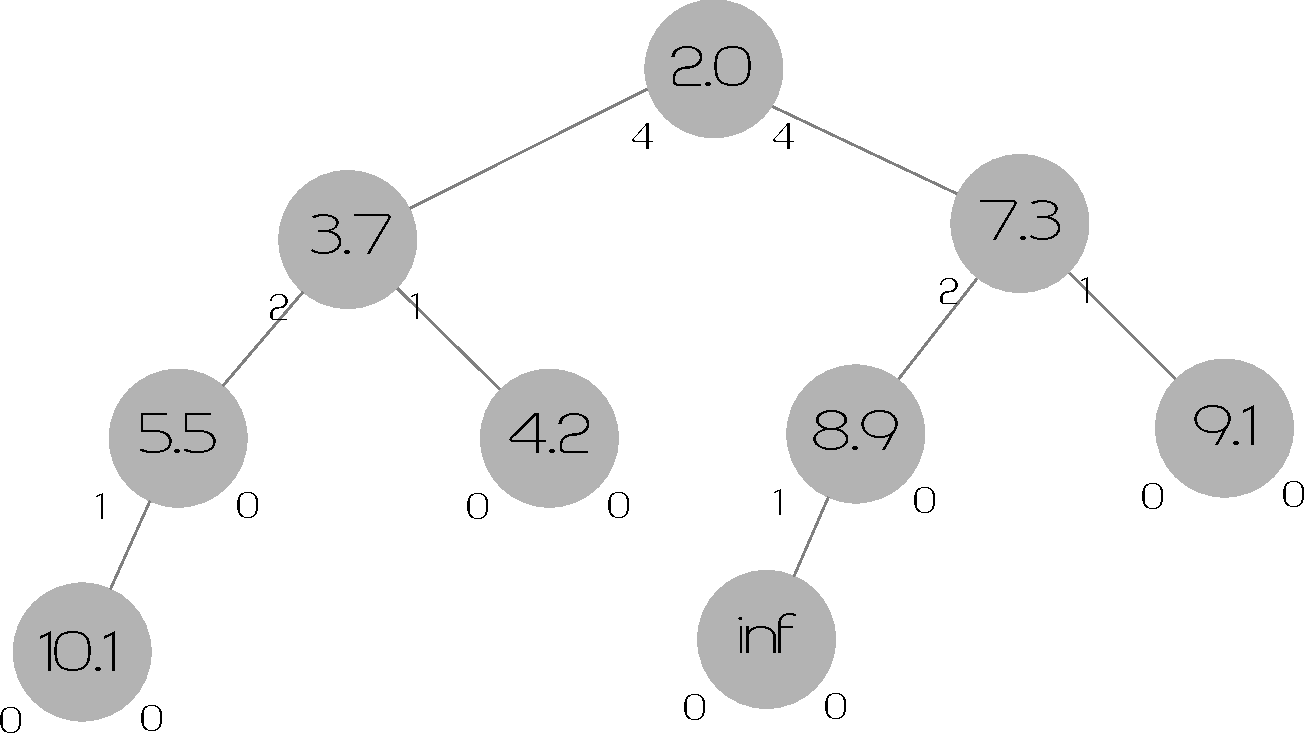
\includegraphics[width=0.99\textwidth]{img/extipq.pdf}
    \caption{Indexed Priority Queue extended with descendant count per branch}
    \label{img:ipq}
  \end{center}
\end{figure}

Our idea is, for each node, to keep track of the number of descendant per branch, having in such way the possibility to keep the tree balanced when adding nodes. In \Cref{img:ipq} we show how the same IPQ drawn in \cite{gibson2000} would appear with our extension. Given this data structure, the procedures to add and remove a new node \texttt{n} are described respectively in \Cref{algo:newnode} and \Cref{algo:remnode}, in which the procedure \texttt{UPDATE\_AUX(n)} is the same described in \cite{gibson2000}.

\begin{algorithm}
\begin{distribalgo}[1]
\vspace{5pt}
\IF{root does not exist}
  \STATE{\texttt{n} is the new root}
\ELSE
  \STATE{\texttt{c} $\gets$ root}
  \WHILE{\texttt{c} has two descendants}
    \IF{\texttt{c.right} $<$ \texttt{c.left}}
      \STATE{\texttt{dir} $\gets$ right}
    \ELSE
      \STATE{\texttt{dir} $\gets$ left}
    \ENDIF
    \STATE{add $1$ to count of \texttt{dir} descendants}
    \STATE{\texttt{c} $\gets$ \texttt{c.dir}}
    \IF{\texttt{c} has not the left child}
      \STATE{\texttt{n} becomes left child of \texttt{c}}
      \STATE{set count of left nodes of \texttt{c} to $1$}
    \ELSE
      \STATE{\texttt{n} becomes right child of \texttt{c}}
      \STATE{set count of right nodes of \texttt{c} to $1$}
    \ENDIF
  \ENDWHILE
  \STATE{\texttt{UPDATE\_AUX(n)}}
\ENDIF
\caption{Procedure to add a new node \texttt{n}}
\label{algo:newnode}
\end{distribalgo}
\end{algorithm}

\begin{algorithm}
\begin{distribalgo}[1]
\vspace{5pt}
\STATE{\texttt{c} $\gets$ root}
\WHILE{\texttt{c} is not a leaf}
  \IF{\texttt{c.left} $>$ \texttt{c.right}}
    \STATE{\texttt{dir} $\gets$ left}
  \ELSE
    \STATE{\texttt{dir} $\gets$ right}
  \ENDIF
  \STATE{subtract $1$ to count of \texttt{dir} descendants}
  \STATE{\texttt{c} $\gets$ \texttt{c.dir}}
\ENDWHILE
\IF{\texttt{c} $\neq$ \texttt{n}}
  \STATE{swap \texttt{n} and \texttt{c}}
  \STATE{remove \texttt{n}}
  \STATE{\texttt{UPDATE\_AUX(c)}}
\ELSE
  \STATE{remove \texttt{n}}
\ENDIF
\caption{Procedure to remove a node \texttt{n}}
\label{algo:remnode}
\end{distribalgo}
\end{algorithm}

Using the two procedures described above, the topology of the whole tree is constrained to remain balanced despite the dynamic addition and removal of reactions.

\chapter{Meta-meta model}
\label{meta-meta-model}
The complexity of the systems we want to design is achieved by the following set of common key properties:
\begin{itemize}
 \item situatedness -- they deal with spatially- and possibly socially-situated activities of entities, and should therefore be able to interact with a limited portion of the surrounding world and contextualise their behaviour accordingly; 
 \item adaptivity -- they should inherently exhibit properties of autonomous adaptation and management to survive contingencies without external intervention, global supervision, or both; 
 \item self-organisation -- spatial and temporal patterns of behaviour should emerge out of local interactions and without a central authority that imposes pre-defined plans.
\end{itemize}

Among the many natural metaphors one can use as inspiration for modelling and developing artificial systems with the above properties \cite{ecosystems-jpcc7}, we consider chemistry following a series of work in the field of pervasive computing \cite{VCMZ-TAAS2011,VZ-INS2010,sapere-procedia7}. 
%
We argue that there are three main issues to be resolved in order to build a meta-model that can be sufficiently expressive for our purpose starting from a purely chemical model:
\begin{enumerate}
 \item the concept of environment where agents are situated and can move is missing in a model that considers only intercommunicating chemical compartments;
 \item the only available mean for changing the system status is the execution of a reaction;
 \item the only data item that chemical reactions can manipulate are molecules' concentrations, namely numbers connected to a particular token.
\end{enumerate}

In the following discussion, we will use interchangeably compartment/agent/node and reaction/events as synonyms.
%
As first step, we introduce the environment, absent in chemistry-derived SSAs, as first class abstraction.
%
The environment has responsibility to provide, for each compartment, a set of compartments that are its neighbours.
%
The rule which is applied to determine whether or not a node belongs to another node's neighbourhood  can be arbitrarily complicated.
%
Also, it is responsible of exposing possible physical boundaries, namely, to limit the possible movements of compartments situated within the environment.

The fact that reactions are the only abstraction the modeller can rely upon in order to let the simulated system progress is not a difficult problem by itself.
%
In fact, nothing prevents to widen the generality of a reaction by defining it as: ``a set of conditions that, when matched, trigger a set of actions on the environment''.

With this definition in mind, a condition is a function that associates to each possible state of the environment a numeric value ranging from zero to positive infinity.
%
If such value is zero, the event can not be scheduled; otherwise, it is up to the reaction to interpret the number: it can influence or not the time at which the reaction will be scheduled, depending on the specific reaction implementation.
%
In case we desire to re-build the original chemical model, we would define a condition for each of the molecules on the left-hand side of the chemical reaction that return the number of molecules currently available in the local compartment.
%
Also, we would define the reaction in such a way that it correctly interprets the number returned by the conditions as concentration of each reactant and correctly applies the rules for computing a propensity to be used to influence the reaction speed \cite{gillespie1977}.

In this framework, actions are arbitrary changes of the environment.
%
In case of pure chemistry, the actions of a reaction would be one for each reactant (that must be removed from the local compartment) and one for each product (that must be added to the local compartment).
%
In case of an extended model considering also multiple compartments, an action should be programmed to be responsible of transferring molecules from a node to a neighbouring one.

Both conditions and actions must expose the set of possible data items (molecules) that they may read or modify: this is necessary in order to allow the dependency graph to be built.
%
Also, both conditions and actions must expose a context of the type \localc{}, \neighborhood{} or \globalc{}; it will be used internally to determine the input and output contexts for the reaction itself.

The reactions are responsible of computing their expected execution time.
%
The engine may require such putative time to be updated in two cases: i) the reaction has just been executed or ii) a reaction on which this reaction depends on has been executed.
%
In case of update required, the reaction should leverage a separately defined time distribution to compute the next putative execution time, possibly feeding the time distribution with a summary of the data gathered from conditions.
%
In case of a Poisson process, a negative exponential time distribution initialised with $\lambda{} = r$ should be used, for instance.
%
In case of a repetitive event, such as a timer, a Dirac comb may be used.

In this model the atomicity of the reactions represent a double edged sword: on the one hand, they allow for arbitrarily complex behaviours to be ordered and executed within a DES, on the other hand they make it difficult to model events that last in time, e.g. to simulate devices with limited computational power on which some complex task takes a not negligible amount of time to get completed.
%
To support something similar, two reactions should be defined: one to trigger the start of the computation, and another to actually run it and complete.

The low expressive power of the classical concentration is probably the hardest challenge to tackle when trying to extend a chemical-born meta model towards a richer world, where data items can be complex structures and not just simple numbers.
%
We have found no trivial solution to this issue; instead, we propose to make the definition ``concentration'' depend on the actual meta-model: let ``concentration'' be ``the data items agents can manipulate''.
%
Besides the trivial example of chemistry, where data items are integer numbers, let's consider a distributed tuple spaces model: in this case, the molecules would be tuples, and the concentration would be defined as ``the set of tuples matching a certain tuple''.
%
Clearly, such flexibility comes with a cost: since the conditions and actions operating on different concentrations dramatically change their behaviour, for any possible class of data items the meta-model must be instanced with a proper set of conditions and actions that can act on such ``concentration''.
%
We call this set of concentration-specific instances of conditions and actions an ``incarnation''.
%
This sort of model inheritance justifies our double ``meta'' level: the model described is a meta-meta-model, an incarnation is a meta-model, and, finally, a specific scenario instancing one of such meta-models is a model.

\label{model}
\begin{figure}%[H]
  \begin{center}
    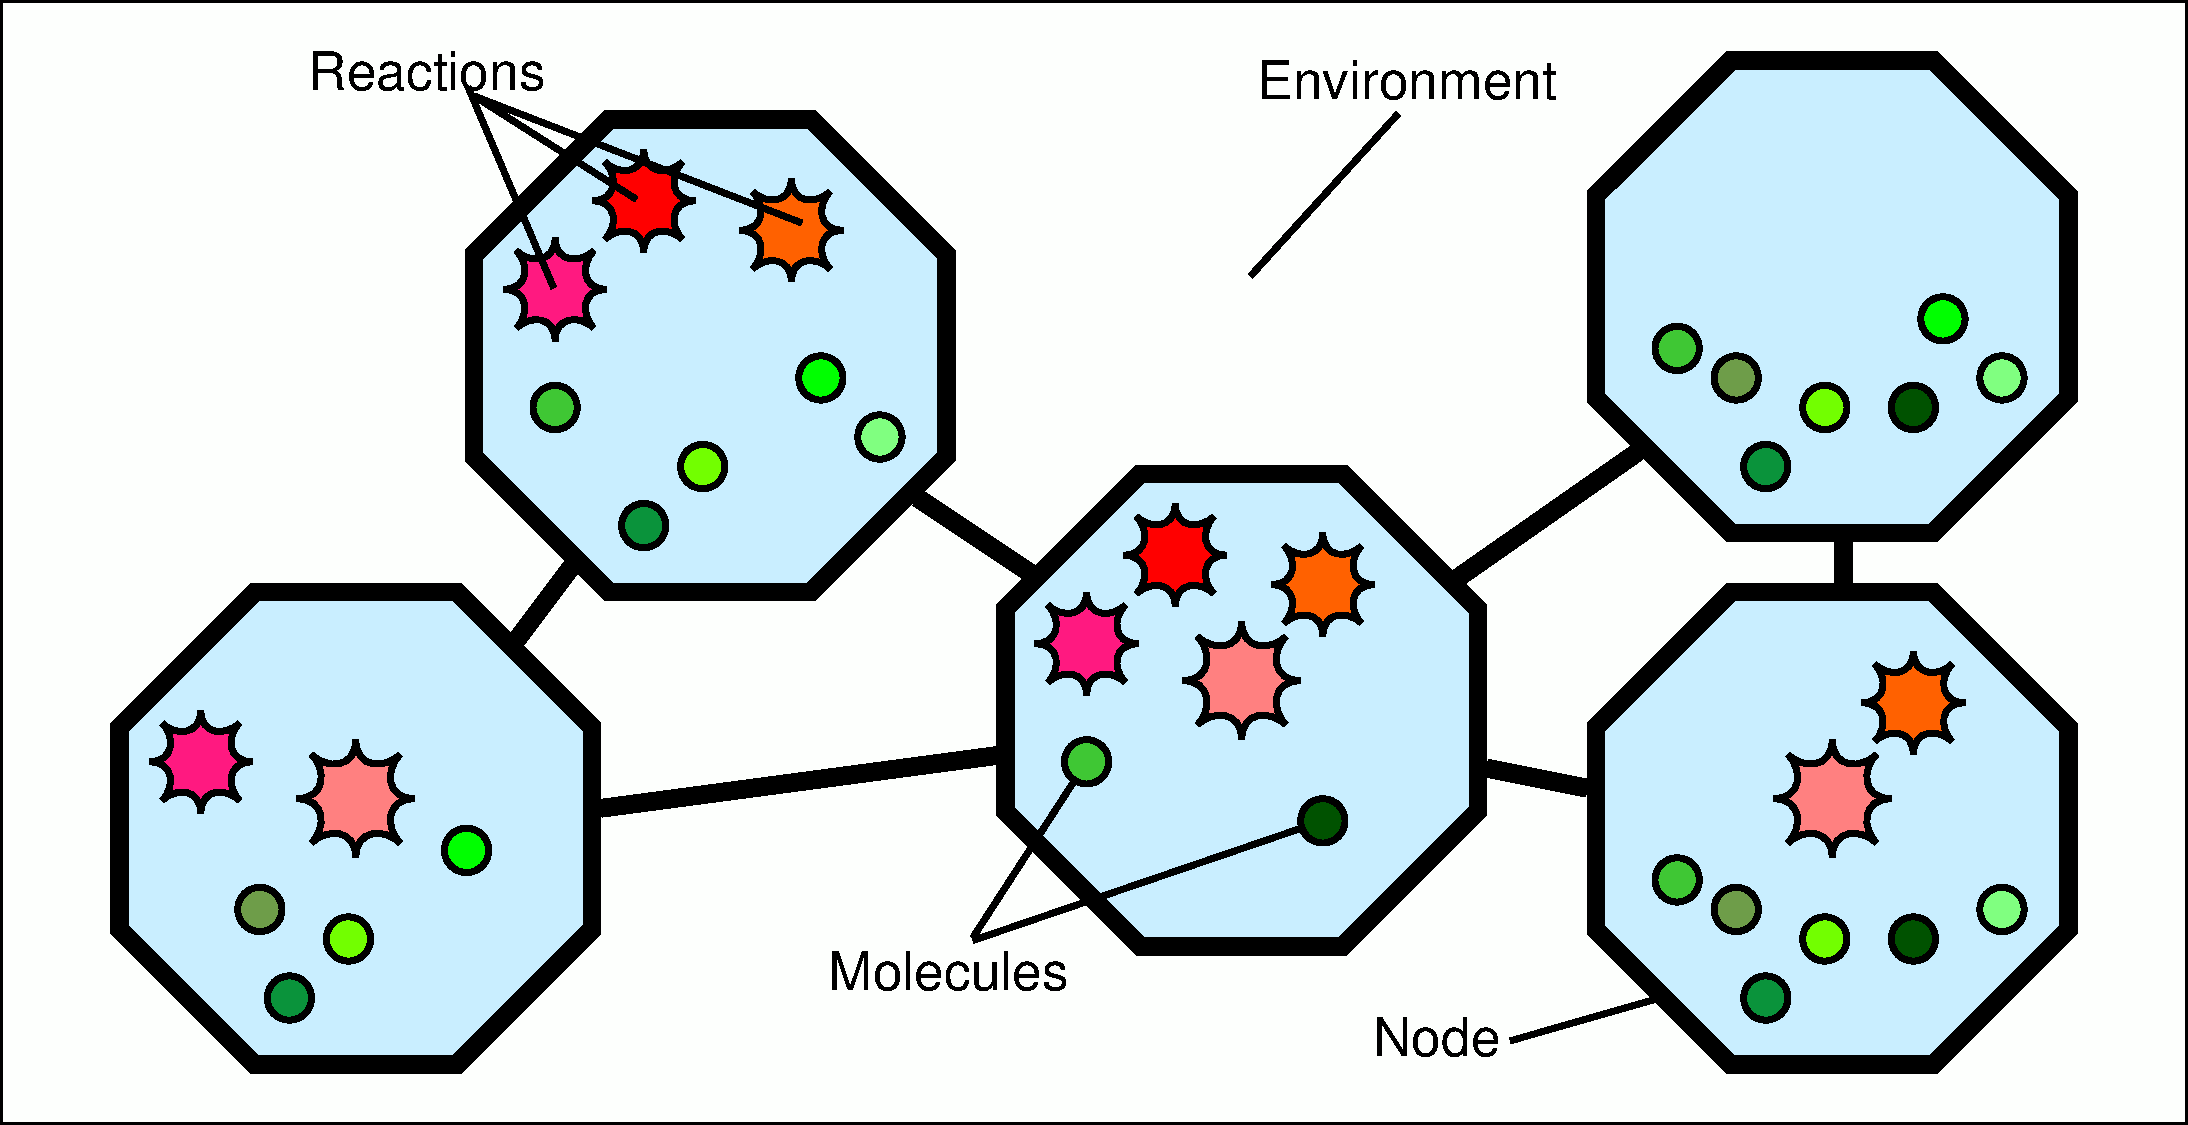
\includegraphics[width=0.99\columnwidth]{img/model.pdf}
    \caption[\alchemist{} computational model]{\alchemist{} computational model: it features a possibly continuous space embedding a linking rule and containing nodes. Each node is programmed with a set of reactions and contains a set of structured molecules.}
    \label{img:model}
  \end{center}
\end{figure}

A pictorial representation of the underlying meta-meta-model is shown in \Cref{img:model}.
%
In this vision of the world, an environment is a multi dimensional space, continuous or discrete, which is able to contain nodes and which is responsible of linking them following a rule.
%
The environment may or not allow nodes to move.
%
Nodes are entities which can be programmed with a set of reactions, possibly changing over time.
%
They also contain molecules, each one equipped with a data structure generalising on the concept of ``concentration''.

\begin{figure*}%[H]
  \begin{center}
    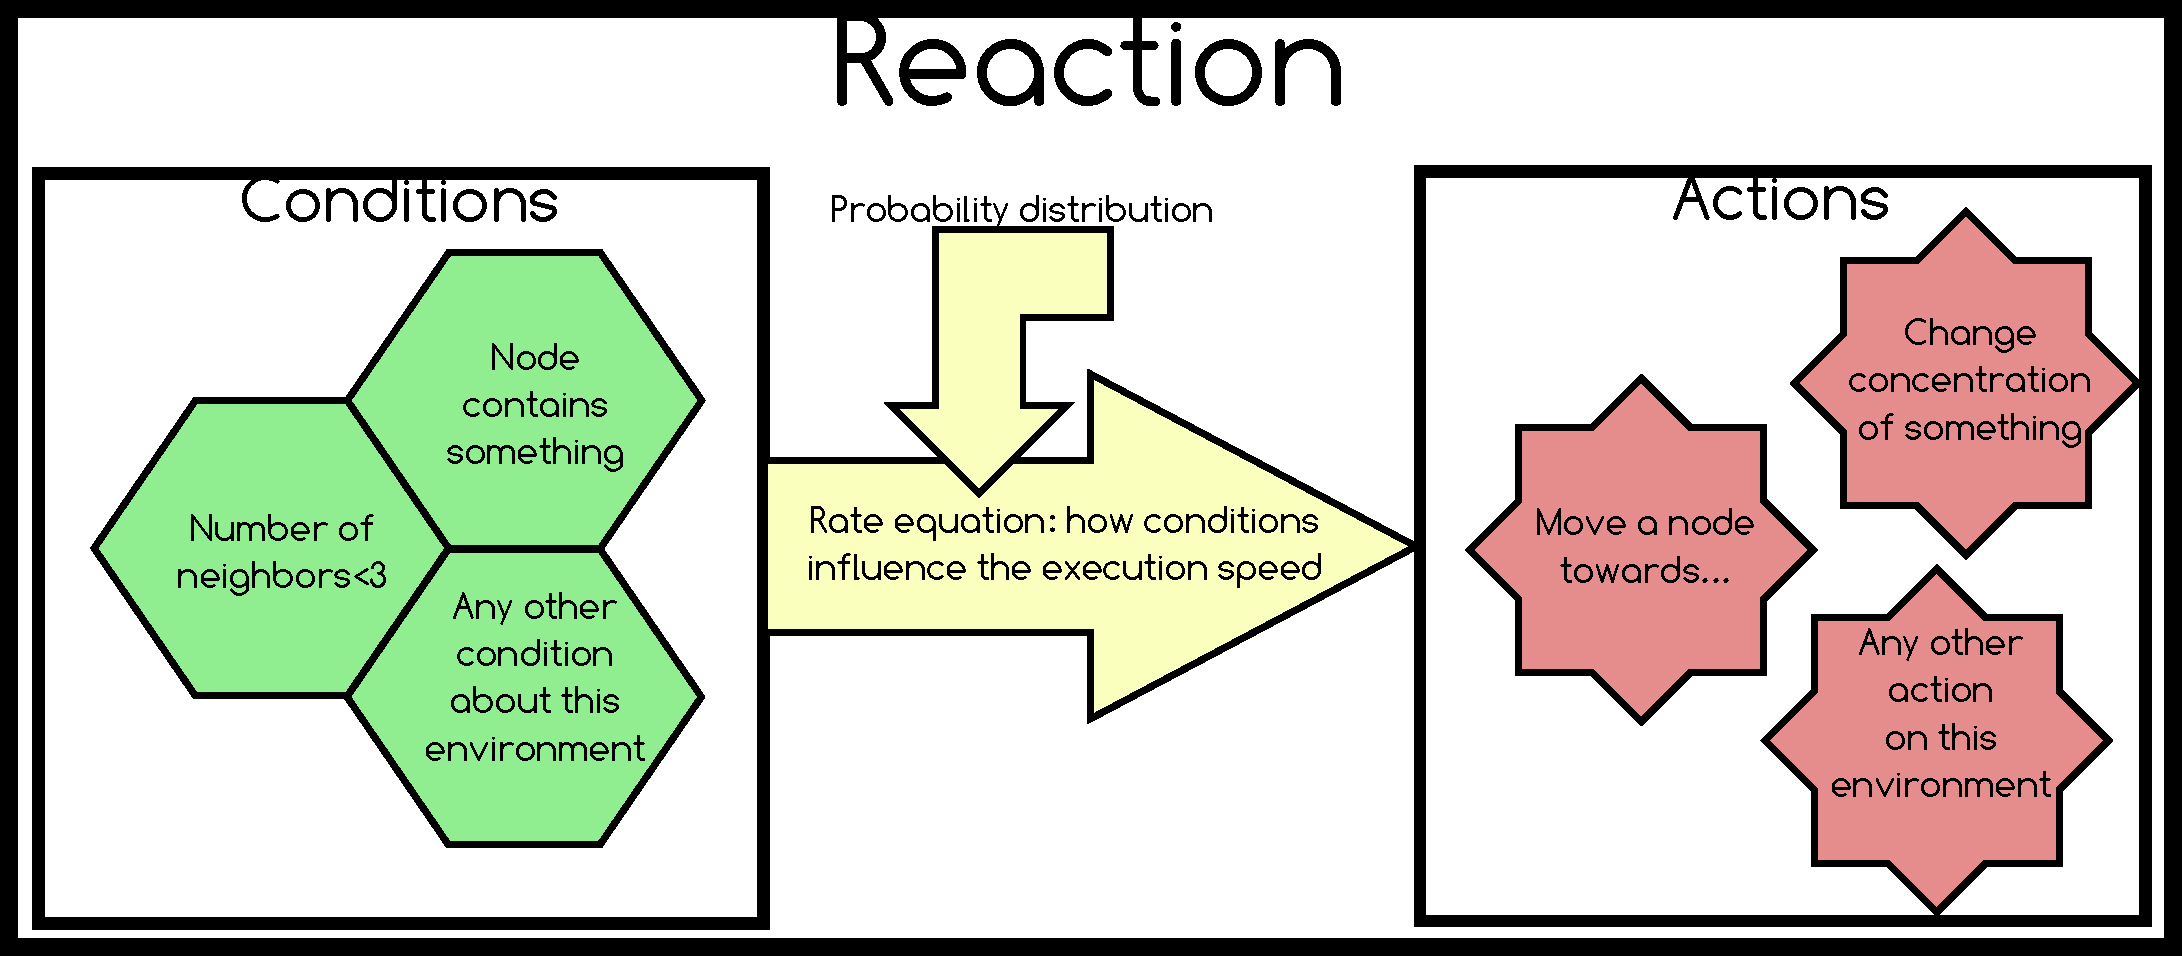
\includegraphics[width=0.99\textwidth]{img/reaction.pdf}
    \caption[\alchemist{} model of reaction]{\alchemist{} model of reaction: a set of conditions on the environment that determines whether the reaction is executable, a rate equation describing how the speed of the reaction changes in response to environment modifications, a probability distribution for the event and a set of actions, which will be the neat effect of the execution of the reaction.}
    \label{img:reaction}
  \end{center}
\end{figure*}

The concept of reaction is graphically depicted in \Cref{img:reaction}.
%
It allows, for example, to model reactions which are faster if a node has many neighbours, or also reactions that resemble complex biological phenomena such as the diffusion of morphogenes during embryo development as described in \cite{LeccaJIB2010}.
%
It also allows to define which kind of time distribution to use to trigger reactions: this enables us to model and simulate systems based on Continuous Time Markov Chains (CTMCs), to add triggers, or also to rely just on classical discrete time ``ticks''.


\chapter{Architecture}
%TODO: architettura da rifare

\label{subsec:architecture}
\begin{figure}%[H]
  \begin{center}
    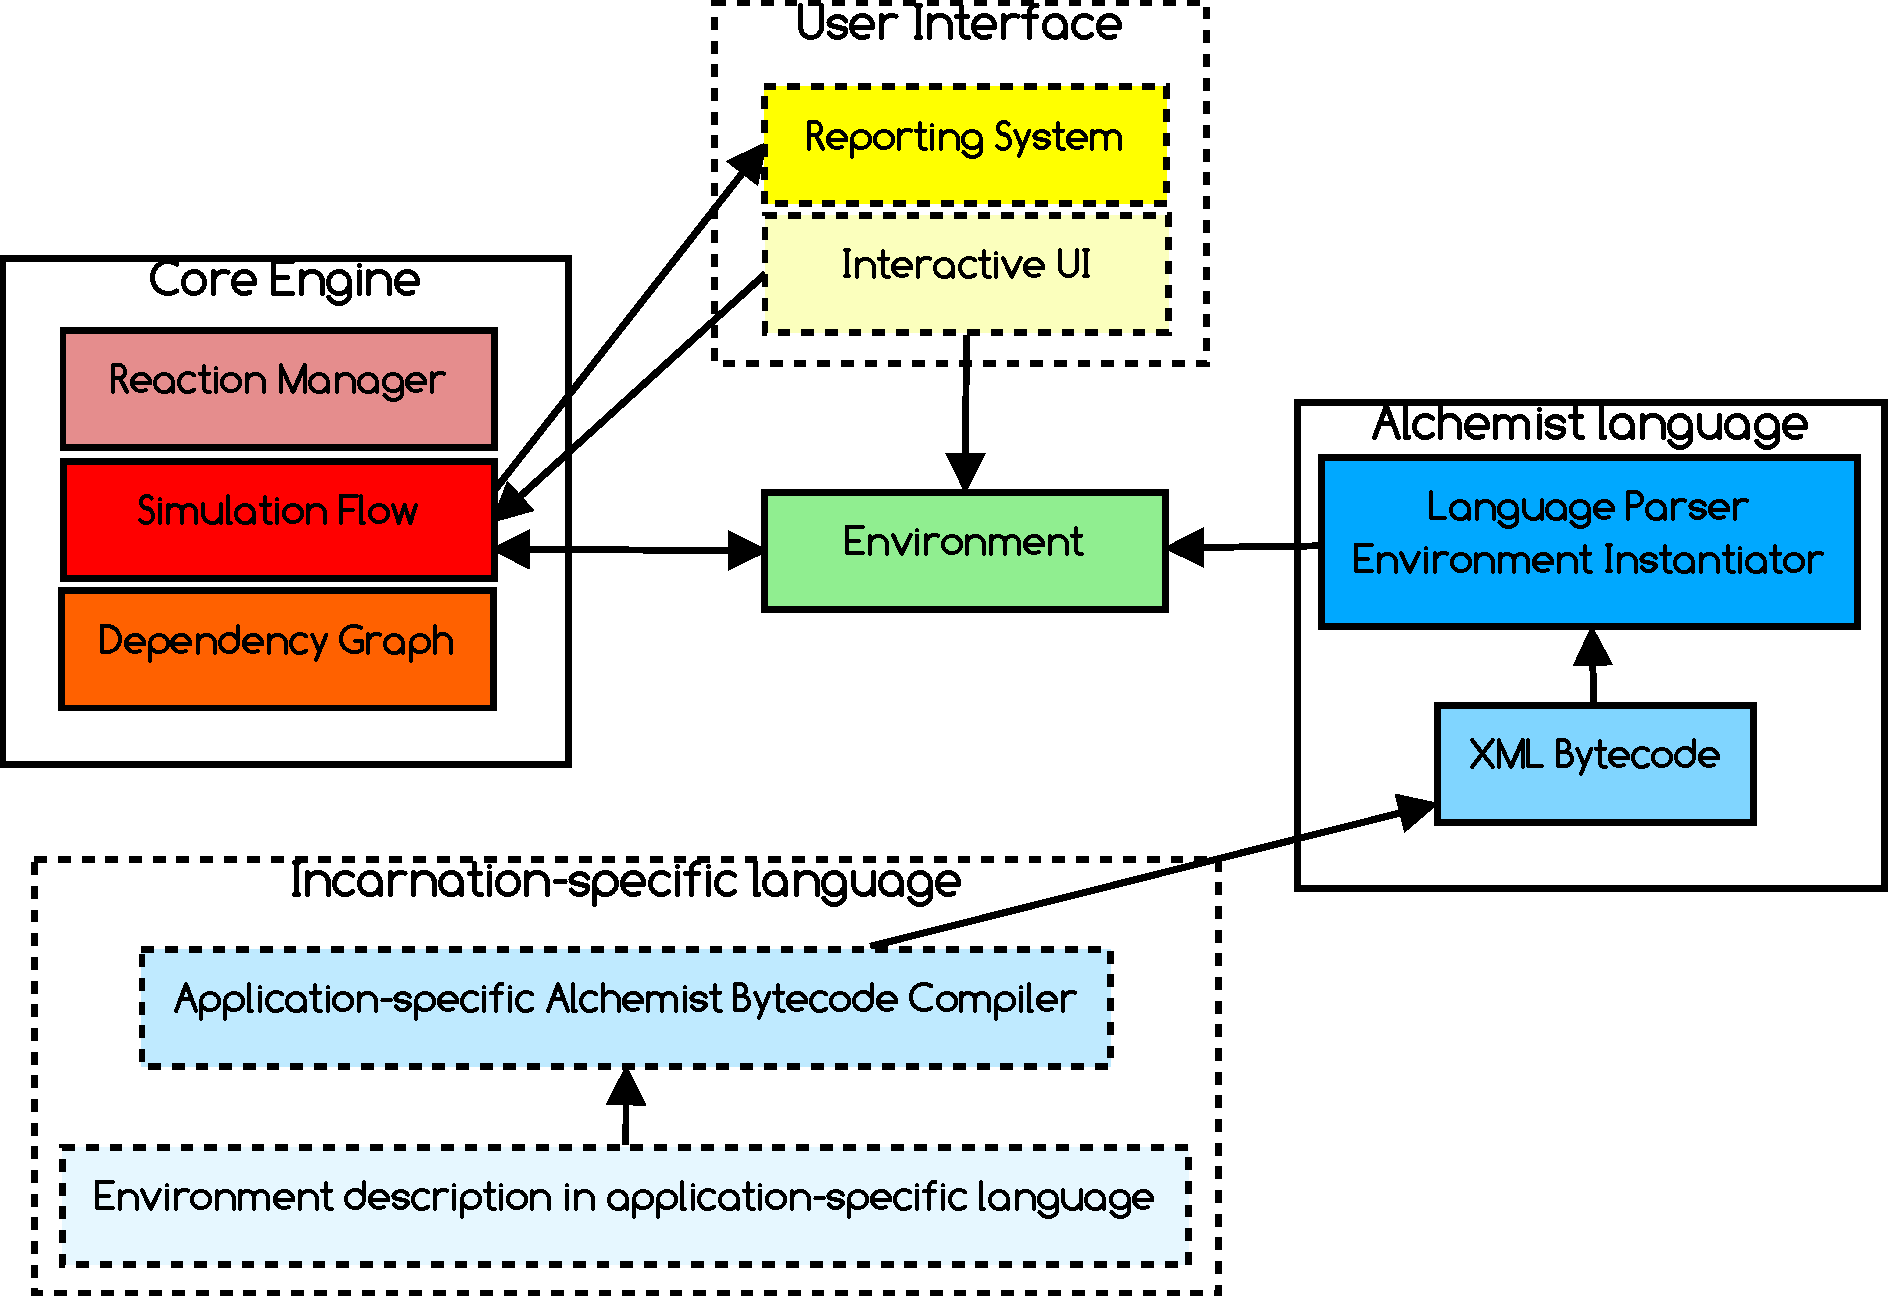
\includegraphics[width=0.7\columnwidth]{img/structure.pdf}
    \caption[\alchemist{} architecture]{\alchemist{} architecture. Elements drawn with continuous lines indicates components common for every scenario and already developed, those with dotted lines are extension-specific components which have to be developed with a specific incarnation in mind.}
    \label{img:arch}
  \end{center}
\end{figure}

The whole framework has been designed to be fully modular and extensible.
The whole engine or parts of it can be re-implemented without touching anything in the model, and on the other hand the model can be extended and modified without affecting the engine.

It is important to note that there is no restriction about the kind of data structure representing the concentration, which can in fact be used to model structured information: by defining a new kind of structure for the concentration, it is possible to incarnate the simulator for different specific uses. For example, by assessing that the concentration is an integer number, representing the number of molecules currently present in a node, \alchemist{} becomes a stochastic simulator for chemistry. A more complex example can be the definition of concentration as a tuple set, and the definition of molecule as tuple template. If we adopt this vision, \alchemist{} can be a simulator for a network of tuple spaces. Each time a new definition of concentration and molecule is made, a new ``incarnation'' of \alchemist{} is automatically defined. For each incarnation, a set of specific actions, conditions, reactions and nodes can be defined, and all the entities already defined for a more generic concentration type can be reused.


%TODO: scrivere una ncarnazione e poi magari anche scrivere una simulazione.

\section{Writing a simulation}

%SISTEMARE%

In order to write a simulation, the user must have, or implement herself, an incarnation of \alchemist{}, as described in \Cref{subsec:architecture}.

As shown in \Cref{img:arch}, the simulations are written in a specific XML language containing a complete description of environment and reactions.
%
This code is interpreted in order to produce an instance of an environment: once it is created, no further interpretation is needed in order to run the simulation.
%
This XML code is not meant to be directly exploited by users: the XML format itself is not exactly human friendly, and XML file is often considerably big (a few megabytes are considered to be normal)
%
However, it is a very standard way of describing environments in a machine-friendly format.
%
The idea behind this choice is that \alchemist{} is flexible enough to be used in various contexts, each one requiring a personalised language and a different instantiation of the meta-model.
%
It is up to the extensor to write a translation module from its personalised language to the \alchemist{} XML.
%
Of course, it is also possible to code the simulation behaviour  directly with Java, although this way exposes the user to many more low level details.

\section{Implementation details}
%TODO%
The framework was developed from scratch using Java. Being performance a critical issue for simulators, we compared some common languages in order to evaluate their performance level.
%
Surprisingly, Java performance are at same level of compiled languages such as C/C++ \cite{bull2003, oancea2011}.
%
The Java language was consequently chosen because of the excellent trade off between performance, easy portability and maintainability of the code, and the high-level support for concurrent programming at the language level. 
%
The COLT Java library\footnote{\url{http://acs.lbl.gov/software/colt/}} provided us the mathematical functions we needed.
%
In particular, it offers a fast and reliable random number generation algorithm, the so called Mersenne Twister \cite{matsumoto1998}.

% TODO! %
\alchemist{} is still actively developed and currently consists of about 200 classes for about 20'000 lines of code. Though still in beta version, it is released with GPL license as open source \footnote{\mbox{\url{http://alchemist.apice.unibo.it}}.}.

\chapter{Performance}
\begin{figure}[t]
    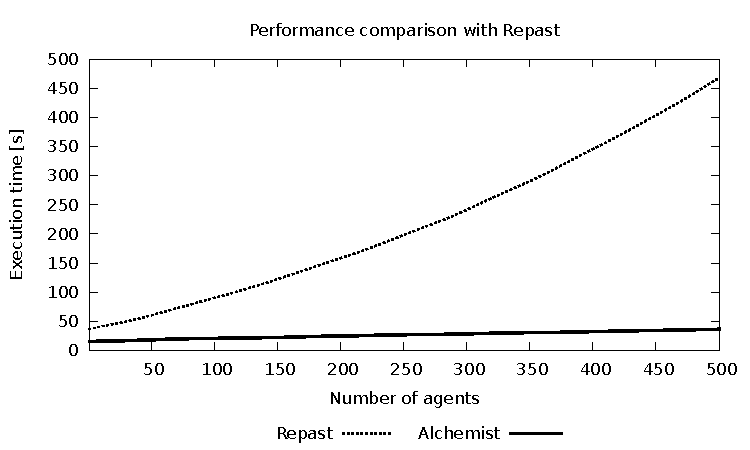
\includegraphics[width=0.999999\columnwidth]{img/jos-graph01}
    \caption{Chart showing the performance scaling of \alchemist{}}
    \label{img:repastperf}
\end{figure}

It is possible to evaluate and compare the performances of \alchemist{} with respect to some known MABS.
%
We exemplify it considering Repast, which we used to developed an alternative simulation for the case study presented in \Cref{jos-museum}\footnote{The source code of the simulation we developed is publicly available at \mbox{\url{http://apice.unibo.it/xwiki/bin/view/Alchemist/JOS/}.}}. There are some important facts that deserve discussion here.

First, since there is no built-in support for stochastic simulation in Repast, we choose to collapse the last five laws of \Cref{img:museum-rules} into a single code path, and the same was made for \alchemist{} by defining a new action.
%
In that way, we were able to avoid for this very specific case the need of a full fledged dependency graph, because there will always be exactly one \textbf{source} and one \textbf{field} per sensor, and no reactions need to be enabled or disabled.
%
This crippled most of the effectiveness of \alchemist{}'s dependency graph, which is indeed a source of optimisation not natively existing in Repast---developing a dependency graph for stochastic simulation in Repast is out of the scope of this thesis, though it would be an interesting subject for future work.
%
On the other hand, it would have been unfair to compare our optimised version against just a plain Gillespie's algorithm built upon Repast.

The second important point is that we choose to encode all the data in both Repast and \alchemist{} as an array of double values instead of real tuples.
%
For \alchemist{}, this meant that we developed a new incarnation for the precise scope of this performance test.
%
The choice of encoding data that way made things faster (no matching required), but also less general.
%
This was done because the SAPERE incarnation of \alchemist{}, which allows us to write the laws as in \Cref{img:museum-rules}, requires a matching system that is not easily portable to Repast.

We choose the configuration of \Cref{img:museum-generalmap2} and we run multiple simulations varying the number of agents per group, in order to evaluate how the two systems scale with the problem size.
%
We measured the running time required to our testbed to run the simulation from the time zero to the time 100.
%
No graphical interface were attached to the simulators while running the batch, in order to evaluate only the raw performance of the engine.
%
The system we used was an Intel Core i5-2500 equipped with 8GB RAM, with Sabayon Linux 7 as operating system and Sun Java HotSpot\texttrademark{} 64-Bit Server version 1.6.0\_26-b03 as Java Virtual Machine.
%
Results are shown in \Cref{img:repastperf}.

Results show the simulator built upon the \alchemist{} framework to be at least twice faster and to scale better than the one built on Repast.
%
Being the dependency graph optimisation cut off as explained above, the reasons for such a difference can lay on the internal scheduler of the engine or in the optimisations in the model.
%
For the first point, we used the default scheduler of Repast Symphony, which is a binary heap implemented through a plain Java array, while our implementation relies on the algorithm and data structures already presented in \Cref{chemical-engine}, so there is not a substantial efficiency difference.
%
For the latter point, a big difference in terms of performances is due to the heavy optimizations of the neighbourhoods of the default \alchemist{} continuous environment.
%
Since the concept of neighbourhood was part of the computational model, it was possible to adopt caching strategies in order to ensure a fast access to the neighbourhood and a quick execution of the operations on it.
%
This is probably the component which gives the highest impact in this case, since most interactions occur among an agent and its neighbourhood.

\chapter{Collocation in literature}

\section{\alchemist{} as a DES}

\alchemist{} is a discrete event simulator (DES), since it combines a continuous time base with the description of system dynamics by distinguished state changes \cite{Zeigler2000}.
%
Since it allows for in-simulation modifications of the environment, it can be considered to belong to the fourth generation of DESs according to \cite{BabulakIJOE2008}.
%
The work in \cite{Pollacia89} surveys the classical DES approaches: according to it, \alchemist{} belongs to the category of simulators featuring ``internal clock'', ``next-event time advance'', and adhering to the ``Event-scheduling World View'', namely, the simulator handles events and is concerned with their effect on system states.

Apart from the meta-model adopted, the main innovative aspect of \alchemist{} with respect to the general DES approach is its ability of optimising the ``compile current event list'' stage \cite{Pollacia89}, which \alchemist{} quickly executes incrementally by means of the management of dependencies that the adoption of a chemical-like model enables.

As far as the simulator model is concerned, instead, the class of DES more related to our approach are those commonly used to simulate biological-like systems.
%
A recent overview of them is available in \cite{EwaldJOS2007}, which takes into account: DEVS \cite{zeigler1984}, Petri Nets \cite{murata1989}, State Charts \cite{Harel1987} and stochastic $\pi$-calculus \cite{Priami1995}.
%
Such an overview however emphasises that all such models require a considerable effort to map biological components into abstractions of the chosen formalism: this is because none of them was specifically developed with biology or bio-inspiration in mind.
%
As described in \Cref{meta-meta-model}, our model is meant to overcome such limitations, since all the enhancements to the basic chemical model we support can be seen as a generalisation of the abstractions of the works presented in \cite{EwaldJOS2007}, and add to them the possibly of customising with much greater flexibility a simulation to the scenarios of bio-inspired computational systems.

We should finally note that the DES approach typically contrasts the use of mathematical techniques (e.g. modelling the system by differential equations).
%
However, the possible different choice of translating a system model to ordinary or partial different equations -- which can be solved numerically in a time considerably shorter than a set of stochastic simulations -- is shown to be impractical in our case.
%
This path, explored for example by \cite{MallavarapuInterface2008}, can provide good results for dynamics that progress at more or less the same speed, and in which abundance of species (data-items or agents in our case) is so high that it can be relaxed to real-valued variables \cite{EwaldJOS2007}.
%
This is not the case for many scenarios even in system biology (see, for example, \cite{Cowan2000, UhrmacherWSC2005}), not to mention scenarios like pervasive computing where reaction rates do not change continuously, and where the effect on an even small number of agents can be key to a given system evolution.

\section{\alchemist{} as a MABS}

Even though chemical-inspired, the meta-meta-model described in \Cref{meta-meta-model} holds evident relationships with multi-agent-based simulation (MABS) approaches.

According to \cite{BandiniJASSS2009}, agent-based platforms for simulations can be split in three categories: general purpose frameworks with specific languages (such as NetLogo), general purpose frameworks based on general purpose programming languages (such as Repast \cite{repast}) and frameworks which provide an higher level linguistic support, often targeted to a very specific application (e.g. \cite{WeynsAAMAS2006}).
%
Each approach has clearly its own advantages and weaknesses.
%
Usually, the more general purpose is the language, the wider is the set of possible scenarios, and the wider is also the gap between the language and the simulated model.
%
This means that an higher level language allows the user to create and tune its simulations in an easier way, on the other hand it often restricts the generality of the tool. 

\alchemist{} is meant to provide a set of meta-models, possibly each with its own domain specific language, still maintaining the possibility to extend or re-implement certain abstractions using the general purpose Java language (defining a new ``incarnation'', namely a new meta-model).

\subsection{Advantages}

There is a set of applications which are better tackled by \alchemist{}.
%
In particular, \alchemist{} is suitable for all those simulation scenarios in which agents have relatively simple behaviour, and the notion of agent-based environment plays instead a fundamental role in organising and regulating the agents' activities \cite{BandiniE4MAS2006} by both enabling local interactions among the proactive entities \cite{HellebooghAAMAS2007} and enforcing coordination rules \cite{aose-mags5}, allowing the modeller to shift her focus from the local behaviour of the single agent to a more objective vision of the whole MAS \cite{SchumacherCEEMAS2007}. 
%
The idea of dealing with a strong notion of environment in multi-agent systems has been deeply developed in a series of work: other than its importance in the simulation context \cite{HellebooghAAMAS2007}, at the infrastructure level \cite{VHRSZ-JAAMAS2007} and at the methodological level \cite{aose-mags5}, there have been proposals of meta-models such as A\&A \cite{artifacts-jaamas17} and infrastructures such as \tucson{} \cite{tucson-aamas99} and \cartago{} \cite{RPV-JAAMAS2011}.
%
A common viewpoint of all these works is that the behaviour of those passive and reactive components structuring the environment (e.g. \emph{artifacts} in A\&A) is well defined in terms of rules expressed as declarative conditions-imply-actions fashion.
%
Accordingly, \alchemist{} is particularly useful either in computing systems following the chemical inspiration \cite{VCMZ-TAAS2011,VZ-INS2010,sapere-procedia7}, or for agent-oriented systems where the role of the environment is key, up to be a very dynamic part of the whole system---where network nodes (or, in biological terms, compartments) can move, new nodes can be spawn or be removed from the system, and links can appear or break at runtime as happen e.g. in pervasive computing scenarios \cite{sapere-procedia7}.

\subsection{Limitations}

Inevitably, as an attempt to build a hybrid between agent-based simulators and (bio)chemical simulators, some trade-offs had to be accepted, which ultimately makes \alchemist{} less suited for certain classes of applications.
%
In particular, a limitation is that \alchemist{}'s agent actions have to be mapped onto the concept of reaction. 
%
On the one hand, this makes it rather straightforward to create reactive memoryless agents \cite{BandiniJASSS2009}, whose goal is just to perform rather easy computations resulting in the creation, deletion or modification of information items in the environment.
%
In fact, since it is allowed to program different nodes with different reactions, it is easy to code reactive and context-dependent agents. On the other hand, there is neither out-of-the-box facility nor any high level abstraction useful to define intelligent agents \cite{BandiniJASSS2009}. The simulator is able to run them provided the user manually writes their whole behaviour as a single Java-written reaction---and properly specifies dependencies with other reactions.
%
Although possible in principle, performing this task too frequently is likely breaking the \alchemist{} abstraction, making the programmer losing the nice declarative approach that chemistry endorses, and possibly hampering the optimisation techniques that motivated \alchemist{}.

\chapter{Meta-model agnostic features}

This\levelText{}analyses the main features of \alchemist{} that can be exploited regardless the specific ``incarnation''.
%
They add a great value to the tool, since they can be used immediately after the creation of a novel meta-model, with no need to specifically write any new code besides some minimal glue.

\section{Distributed statistical analysis}

As we have seen in \Cref{engineering-and-tools}, simulation represents a key step in the engineering of pervasive systems.
%
Being a simulation basically a sampling over an enormous probability space, obvious questions accompany these procedures:
\begin{itemize}
 \item how reliable are the obtained values?
 \item How is the number of performed simulations chosen?
 \item How many simulations are required in order to state system properties with a certain degree of confidence?
\end{itemize}

Moreover, there is frequently a lack of decoupling between the model specification and the definition of the system's properties of interest: they are often embedded in the model, and their values are obtained via logging operations performed during the simulation process.

This\levelText{}presents a tool meant to face these challenges, obtained chaining \alchemist{}, with \multivesta{}\footnote{\url{http://code.google.com/p/multivesta/}} \cite{multivesta}, a recently proposed lightweight tool extending \vesta{}~\cite{Sen:2005} and \pvesta{}~\cite{AlTurkiM11} which allows to enrich existing discrete event simulators with automated and distributed statistical analysis capabilities.
%
The result is thus a statistical analysis tool tailored to chemical-inspired pervasive systems.
%
The benefits obtained by chaining the simulator with \multivesta{} are:
\begin{enumerate}
 \item a language (\multiquatex) to compactly and cleanly express systems properties, decoupled from the model specification;
 \item the automated estimation of the expected values of \multiquatex{} expressions with respect to \emph{n} independent simulations, with \emph{n} large enough to respect a user-specified confidence interval;
 \item an interactive plot as well as the generation of gnuplot input files to visualize the obtained results;
 \item a client-server architecture to distribute simulations.
\end{enumerate}

\multivesta{} is independent on the model specification language: it only assumes that discrete event simulations can be performed on the input model.
%
As described in~\cite{multivesta}, the tool offers a clean interface to integrate existing discrete event simulators, enriching them with a property specification language, and with efficient distributed statistical analysis capabilities.

\subsection{\multivesta{} and \multiquatex{}}

\multivesta{} performs a statistical (Monte Carlo based) evaluation of \multiquatex{} expressions, allowing to query about expected values of observations performed on simulations of probabilistic models. 
%
A \multiquatex{} expression may regard more measures of a model, in which case the same simulations are reused to estimate them, thus improving the performance of the analysis tasks. %
Moreover, the tool has a client-server architecture allowing to distribute the simulations on different machines.
%
A detailed description of \multiquatex{} and of the procedure to estimate its expressions is out of the focus of this work, the interested reader can deepen her knowledge reading \cite{multivesta,AghaMS06}.
%
Before defining a \multiquatex{} expression, it is necessary to specify the state characteristics to be observed.
%
This model-specific step ``connects'' \multiquatex{} with the model.
%
The state observations are offered via the \texttt{{rval}}(\emph{obs}) predicate which returns a real number for each observation, specified by the string parameter \emph{obs}. 

A \multiquatex{} expression consists of a set of definitions of \emph{parametric recursive temporal operators}, followed by a list of \emph{\texttt{eval} clauses}. Each \texttt{eval} clause relies on the defined temporal operators, and specifies a property whose expected value must be evaluated.

In order to evaluate a \multiquatex{} expression, \multivesta{} performs several simulations, obtaining from each a list of samples (real numbers).
%
One sample for each \texttt{eval} clause is obtained, thus all the queried measures are evaluated using the same simulations, improving performance.
%
Based on the samples obtained from simulations, \multivesta{} estimates \multiquatex{} expressions with respect to two user-provided parameters: $\alpha$ and $\delta$. 
%
Considering the case of simple expressions with just one \texttt{eval} clause, the estimations are computed as the mean value of the $n$ samples obtained from $n$ simulations, with $n$ large enough to grant that the size of the $(1 - \alpha)*100\%$  \textit{Confidence Interval} (CI) is bounded by $\delta$.
%
In other words, if a simple \multiquatex{} expression is estimated as $\overline{x}$, then, with probability $(1 - \alpha)$, its actual expected value belongs to the interval $[\overline{x} - \delta/2,\overline{x} + \delta/2]$.
%
The case of expressions with multiple \texttt{eval} clauses is similar, with the note that the \texttt{eval} clauses may regard values of different orders of magnitude, and thus the user may provide a list of $\delta$ rather than just one. 
%
After having obtained a sample for every \texttt{eval} clause from a simulation, these values are used to update the means of the samples obtained from previous simulations (one mean per \texttt{eval} clause). If the CIs have been reached for every \texttt{eval} clause, the evaluation of the expression is terminated, otherwise further simulations are performed.
%
Note that each \texttt{eval} clause may require a different number of simulations to reach the required CI. Once the CI of an \texttt{eval} clause has been reached, such \texttt{eval} clause is ignored in eventual further simulations performed for other \texttt{eval} clauses. 


\subsection{Integrating \multivesta{} and \alchemist{}}

In order to chain the tools, some steps, have been tackled once and for all, while others are model-specific.
%
Essentially, in order to allow the interaction with \multivesta{}, \alchemist{} has to fulfill two requirements:
\begin{enumerate}
 \item the ability to advance the simulation in a step-by-step manner (which is provided by the \texttt{playSingleStepAndWait} method in \texttt{ISimulation} interface);
 \item the ability to analyze the model status after each simulation step, providing measures in form of real numbers about properties of interest.
\end{enumerate}

Since both \multivesta{} and \alchemist{} are Java-based, their interaction has been easily realized by subclassing the \texttt{NewState} class of \multivesta{}.
%
The obtained \texttt{AlchemistState} class is sketched in \Cref{lst:alchemiststate}, where unnecessary details are omitted.
The new class contains some \alchemist{}-specific code, providing \multivesta{} with the simulation control and proper entry points for the analysis.

\begin{lstlisting}[frame=single, basicstyle=\scriptsize, language=Java, mathescape, caption=AlchemistState extending \multivesta{}'s NewState class, label=lst:alchemiststate,float=t,numbers=left]
public class AlchemistState<N extends Number, D extends Number, T> extends NewState {
  private final long maxS; 
  private final ITime maxT;
  private ISimulation<N, D, T> sim;
  ...
  public AlchemistState(final ParametersForState params) throws ...{
    super(params);
    final StringTokenizer otherparams = new StringTokenizer(params.getOtherParameters());
  /* Initialization of Alchemist-specific parameters
     and execution environment resorting to otherParams */
  }
  ...
  public void setSimulatorForNewSimulation(final int seed) {
    /* Stop current simulation, create a new one. */
    ...
    sim.stop();
    ...
    env = getFreshEnvironment(seed);
    sim = new Simulation<>(env, maxS, maxT);
    ...
  }
  ...
  public void performOneStepOfSimulation() {
    sim.playSingleStepAndWait();
  }
  ...
  public double rval(final String obs) {
    if(obs.equals("time")) return getTime();
    if(obs.equals("steps")) return getStep();
    //other model-independent observations 
    ...
    return getStateEvaluator().getVal(obs, this);
  }
}
\end{lstlisting}

In the constructor (lines $6$-$10$), the superclass initialization is done by a simple \texttt{super()} call.
%
The remaining code initializes \alchemist{}-specific parameters such as the maximum time or steps to simulate.
%
Those  are in general not required, since \multivesta{} is able to detect when the analysis requirements have been met, and consequently stop the simulation flow.
%
The method \texttt{setSimulatorForNewSimulation()} is depicted in lines $12$-$20$.
%
The method is invoked by \multivesta{} before performing a new simulation to (re)initialize the status of the simulator, providing to it a new random seed. 
%
In lines $22$-$24$, \texttt{performOneStepOfSimulation()} is provided: resorting to the \alchemist{} method \texttt{playSingleStepAndWait()}, it allows \multivesta{} to order the execution of a single simulation step.

In order to inspect the simulation state, the \texttt{rval()} method defined in lines $26$-$32$ is invoked.
%
The argument specifies the observations of interest.
%
This method inspects the simulation state for all aspects common to any \alchemist{} model, e.g., in the listing are sketched the current simulated time (line $27$) and the number of performed simulation steps (line $28$).
%
Clearly, each \alchemist{} model will have its own observations of interest.

Depending on the model at hand, it may be necessary to refine the model-independent observations exposed by \texttt{AlchemistState} with a set of model-specific ones. This can be done by simply instantiating the \texttt{IStateEvaluator} interface provided by \multivesta, constituted by one method only.

\subsection{Example}

This\levelText{}discusses the analysis performed on a crowd steering scenario, similar to the one which will be presented in detail in \Cref{jos-museum}.
%
In such scenario, two group of people are inside an indoor environment, and are steered towards two point of interest (POI) such that their ideal trajectory intersect, creating a crowd.
%
The steering system is implemented leveraging the SAPERE meta-model, and as such data items in this scenario are called \texttt{LSA}s.
%
This example is not meant to provide significant scientific insights on crowd steering (thoughts about it will be provided in the remainder of this thesis), but rather to act as toy-example to demonstrate the flexibility and possibilities of the chaining of \alchemist{} and \multivesta{}.

The outcome of the analysis is summarized in the three charts of \Cref{img:analysisCharts} (obtained using the gnuplot input files provided by \multivesta{}), showing, at the varying of the simulated time, the expected values of: the number of people which have reached their point of interest (top), the average number of connections of the devices (middle), and the number of LSAs in the system (bottom).

\lstset{caption=The evaluated parametric multi-expression ($MainMQ$), label=listing:parametricMQ}
\begin{lstlisting}[frame=single, mathescape, morekeywords={parametric,eval,E,if,fi,then,else,s,rval,evalME,evalOnceME}, float=t, numbers=left]
people@POI($x$) = if{s.rval("time") >= $x$}
      then s.rval("bPOI")
      else $\textbf{{\#}}$people@POI($x$)
   fi;
people@RPOI($x$) = // similar to people@POI
people@LPOI($x$) = // similar to people@POI
avgConn($x$) = if{s.rval("time") >= $x$}
      then s.rval("degree")
      else $\textbf{{\#}}$avgConn($x$)
   fi;
LSAs($x$) = if{s.rval("time") >= $x$}
      then s.rval("LSAs") 
      else $\textbf{{\#}}$LSAs($x$)
fi;
eval parametric(E[people@POI($x$)],E[people@RPOI($x$)],              E[people@LPOI($x$)],E[avgConn($x$)],E[LSAs($x$)],$x$,$0.0$,$1.0$,$50.0$);
\end{lstlisting}

The three charts have been obtained by evaluating $MainMQ$ of \Cref{listing:parametricMQ}, having $5$ parametric temporal operators (lines $1$-$9$):
%
\texttt{people@RPOI} and \texttt{people@LPOI} regard the number of people which have reached, respectively, the POI on the right and the one on the left, while \texttt{people@POI} counts instead how many people have reached their destination. The fourth temporal operator (\texttt{avgConn}) regards the connectivity degree of the devices. Finally, \texttt{LSA}s regards the number of LSA in the system, giving insights on the amount of memory required to sustain the system.
%
The temporal operators are analysed at the varying of the simulated time from $0$ to $50$ seconds, with step $1$ (line $10$). Thus the analysis consisted in the estimation of the expected values of the $5$ temporal operators instantiated with $50$ parameters, for a total of $250$ expected values. 

\begin{figure}
\begin{center}
\vspace{-0.2cm}
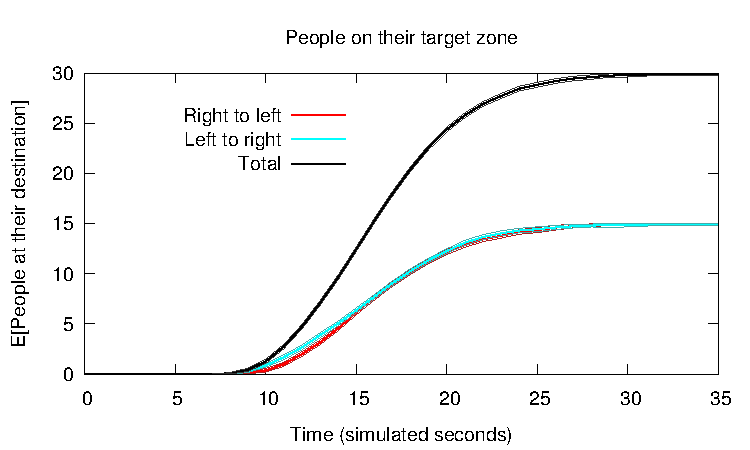
\includegraphics[width=0.7\columnwidth]{img/people}
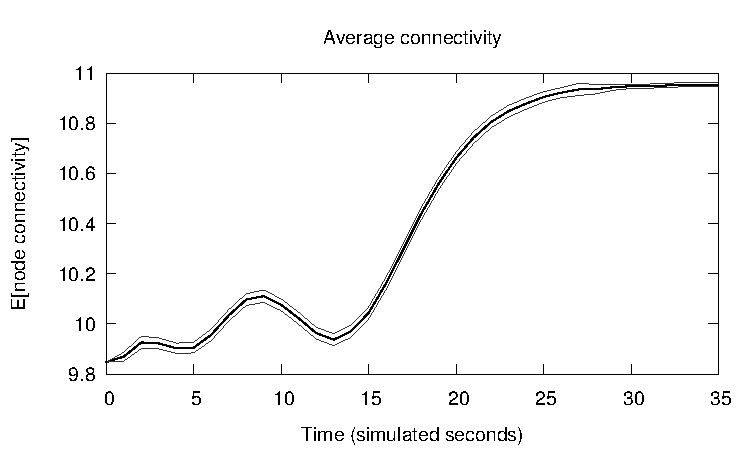
\includegraphics[width=0.7\columnwidth]{img/connectivity}
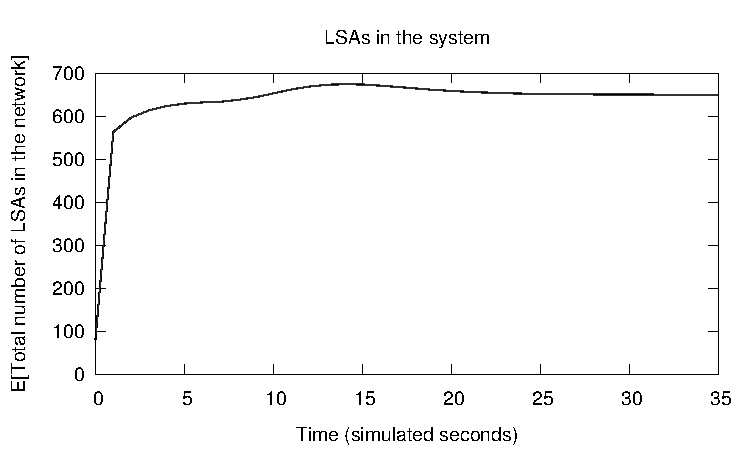
\includegraphics[width=0.7\columnwidth]{img/lsas}
\caption[Analysis of a crowd steering scenario with \alchemist{} and \multivesta]{Analysis of the crowd steering scenario: (top) number of people at the POIs, (middle) average number of connections per device, (bottom) number of LSAs in the system.}
\label{img:analysisCharts}
\end{center}
\end{figure}

A high degree of precision has been required: $\alpha$ has been set to $0.01$, while the $\delta$ values (the size of the CIs) have been chosen considering the orders of magnitude of the measures: $0.5$ for the instances of \texttt{people@POI($x$)}, \texttt{people@RPOI($x$)} and \texttt{people@LPOI($x$)}; $0.05$ for  \texttt{avgConn($x$)}; and $3$ for \texttt{LSAs($x$)}.
%
To reach such a level of confidence, the tool ran approximately $2500$ simulations, requiring less than a hour.
%
The discussed confidence intervals are depicted in the aforementioned charts: the two lines drawn above and below the central lines represent the obtained CIs of the expected values, thus indicating the intervals in which the actual expected values lie with probability $0.99$.

The top chart regards the first $3$ temporal operators: the top plot refers to the number of people in total which have reached their target POI, while the two almost over-imposed lower plots regard the number of people at the right POI and at the left POI. 
%
All the three measures under analysis produced monotonically increasing sigmoid curves.
%
We can deduce from this behavior that there are no systemic errors in the crowd steering system, such as people with no or wrong suggested final destination, in which case we would have noticed one or more flatted zones flawing the sigmoid curve.
%
We note also that after around 30 simulated seconds all the people have reached their target, and that it takes around 10 seconds for the fastest walkers to get to their destination.
Note that, despite that the analysis has been performed for 50 simulated seconds, the charts presented in \Cref{img:analysisCharts} have been cut at time 35 to better show the most relevant results: in fact, the system reaches stability after this time, and no event of interest happens later.
%
Moreover we can also notice that people going from left to right are slightly faster than the other group.
%
This difference, due to the asymmetric positioning of people in the center of the scenario, is hardly visible and would have been impossible to spot with a lower precision analysis.

The middle chart shows the evolution in time of the average number of connections of the devices (i.e., both sensors and smartphones).
%
Since each device is considered to be connected to all those within a range of 1.5 meters, it also gives us a hint about the crowding level.
%
There is a noticeable peak at around 8 seconds: it is due to a high number of people approaching the central group.
%
After that, the peak disappears when most people overtook the obstacle and are walking towards their POI.
%
Finally, there is a growth: progressively, people reach their destination and tend to create a crowd.

The bottom chart shows the number of LSAs in the whole system, indirectly giving hints on the global memory usage.
%
Once the system is started, there is a very quick growth, due to the gradient being spread from the sources to the whole sensors network and to the LSAs produced by the crowd-sensing.
%
The system reaches a substantial stability after a couple of seconds.
%
From that point on, the number of LSAs has very little variations: the system has no ``memory leak'', in the sense that it does not keep on producing new LSAs without properly removing old data. 

\subsection{Performance Assessment}
All the experiments of the previous section have been run on a machine equipped with four Intel\textregistered{} Xeon\textregistered{} E7540 and 64GB of RAM, running Linux 2.6.32 and Java 1.7.0\_04-b20 64bit.

In order to measure the performance scaling of the tool, we ran our analysis multiple times varying the number of \multivesta{} servers deployed.
%
Results are summarized by the dark line of \Cref{img:performance}, showing that with only 1 server (\alchemist{} does not have any parallel capability by its own), the analysis required almost 17 hours, while with more than 30 servers (enabled by the chaining with \multivesta{}) it required less than an hour. For the considered scenario, by distributing simulations we have thus obtained a more than eighteen times faster analysis.

\begin{figure}[t]
\begin{center}
\vspace{-0.2cm}
%  \includegraphics[width=0.49\textwidth]{charts/perfcomp}
 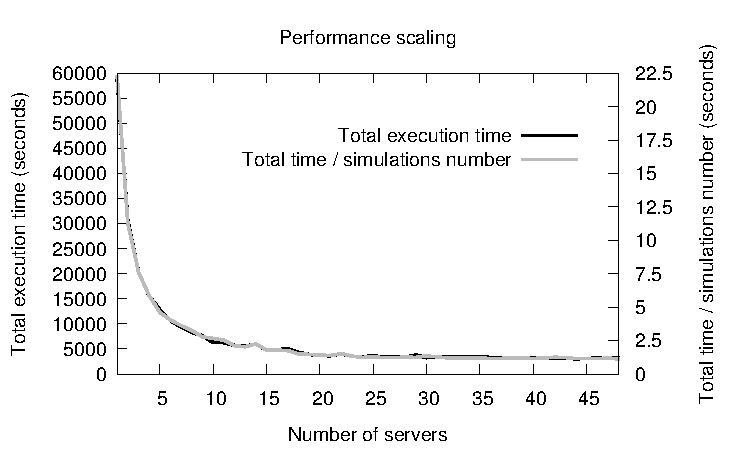
\includegraphics[width=0.99\textwidth]{img/scaling}
 \end{center}
%  \caption{Performance improvement reusing simulations (left), performance scaling a the varying of the number of used cores (right).}
 \caption{Performance scaling with of the number of running servers.}
 \label{img:performance}
\end{figure}

It is worth to note that such comparison of performance is affected by the statistical nature of the analysis procedure. 
%
Intuitively, when evaluating a \multiquatex{} expression resorting to $x$ or to $x + y$ servers, in both cases we initialize the first $x$ servers with the same $x$ seeds, generating thus the same $x$ simulations. However, the remaining $y$ servers are initialized with new seeds, and thus produce new simulations.
Clearly, by having different simulations, we may obtain different sample variances, requiring a different number of simulations.
%
For this reason, the bright line of \Cref{img:performance} depicts the time analysis normalized with respect to the number of simulations (obtained dividing the overall analysis time by the number of performed simulations).
%
The two lines of \Cref{img:performance} evolve accordingly, thus confirming the great performance gain brought by the distribution of simulations.

\begin{table}[tb]
 \caption{Time performance improvements reusing simulations (seconds).}
%\begin{figure}[t]
%\caption{{Performance improvements reusing simulations. Times are in seconds.}}
\begin{center}
\scalebox{0.82}{
 \begin{tabular}{| c | c | c | c |}
 \hline
 %\hline
 & \textbf{Expressions} & \textbf{Param. expressions} & \textbf{Param. multi-expressions} \\
 \hline%\hline
 \textbf{\texttt{people@POI}} & 
 %THIS IS THE CORRECT NUMBER { 28045.77}
 28045.77
 %39999.32 %IN THE PAPER SUBMITTED TO 4PAD WE DISCUSSED THIS 
 & 2567.26 & n.a. \\
 \hline
 \textbf{\texttt{people@RPOI}} & 15891.13 & 1114.86 & n.a. \\
 \hline
 \textbf{\texttt{people@LPOI}} & 15560.83 & 950.30 & n.a. \\
 \hline
 \textbf{\texttt{avgConn}} & {%\color{blue}
 90111.29}  % 
 & 1372.64 & n.a. \\
 \hline
 \textbf{\texttt{LSAs}} & 58630.45 %1m11.231 
 & 2504.33 & n.a. \\
 \hline\hline
 \textbf{Total time} & {%\color{blue}
 %220193.02
  208239.47
 } & 8509.39 & 3215.95 \\
 \hline
 %\hline
 \end{tabular}}
\end{center}
 %\caption{Time performance improvements reusing simulations (seconds).}
 \label{tab:reuse}
%\end{figure}
\end{table}

\multivesta{} has a further important feature which dramatically reduces the analysis time: the reuse of simulations to estimate many expected values. 
%
The reusage happens on two levels:
\begin{enumerate}
 \item expressions can be made parametric, and thus simulations can be reused for computing the same property at the varying of a parameter (e.g., at different time steps);
 \item it is possible to write multi-expressions , and thus reuse simulations to evaluate multiple properties.
\end{enumerate}
%
Moreover,  by combining these two features, it is possible to reuse simulations for multiple parametric properties (e.g. $MainMQ$ of \Cref{listing:parametricMQ}).
%
As explicated by \Cref{tab:reuse} (whose reported analysis have been performed resorting to 48 servers), 	parametric expressions (second column) allowed us to save a stunning {%\color{blue}
96}\% of execution time with respect to the simple expressions case without reuse of simulations (first column). Moreover, the parametric multi-expression feature (third column) allowed us to further cut down this time to a third.
%
We can thus advocate that, by exploiting reuse of simulations, for the considered scenario we obtained a more than 64 times faster analysis.
%
Clearly, the performance gains change depending on the considered scenario or properties. In fact, the more simulations are required, and the longer they take, the greater will be the advantage.

\section{Real world maps}

\alchemist{} supports real-world environments.
%
The base functionality lies in the possibility to load maps and simulate within them.
%
Currently, the simulator supports OpenStreetMap\cite{osm}, and it is able to load data in multiple OSM XML, compressed OSM XML and Protcolbuffer Binary Format (PBF).
%
The latter is warmly recommended for both performance and map file size.
%
Various websites provide ready-to-use extracts of the world map in PBF format for cities and whole regions, and arbitrarily sized extracts in OSM XML format can be obtained via public web API.

Once the map has been loaded, \alchemist{} offers the possibility to enrich the simulations with the maps data, and in particular offers various ways to move nodes within the environment taking into account the characteristics of the map.

The first feature offered is about the initial node displacing.
%
When adding a node to the environment, in fact, it is possible not to displace the node in the exact position indicated, but in the nearest street point.
%
This comes in particularly handy in order to realise the network of static devices: the simulator can be fed with a grid of devices, and it automatically modifies the positions of each node in order to displace it on a street.

 \begin{figure}
 \centering
  \subfigure[GPS trace]{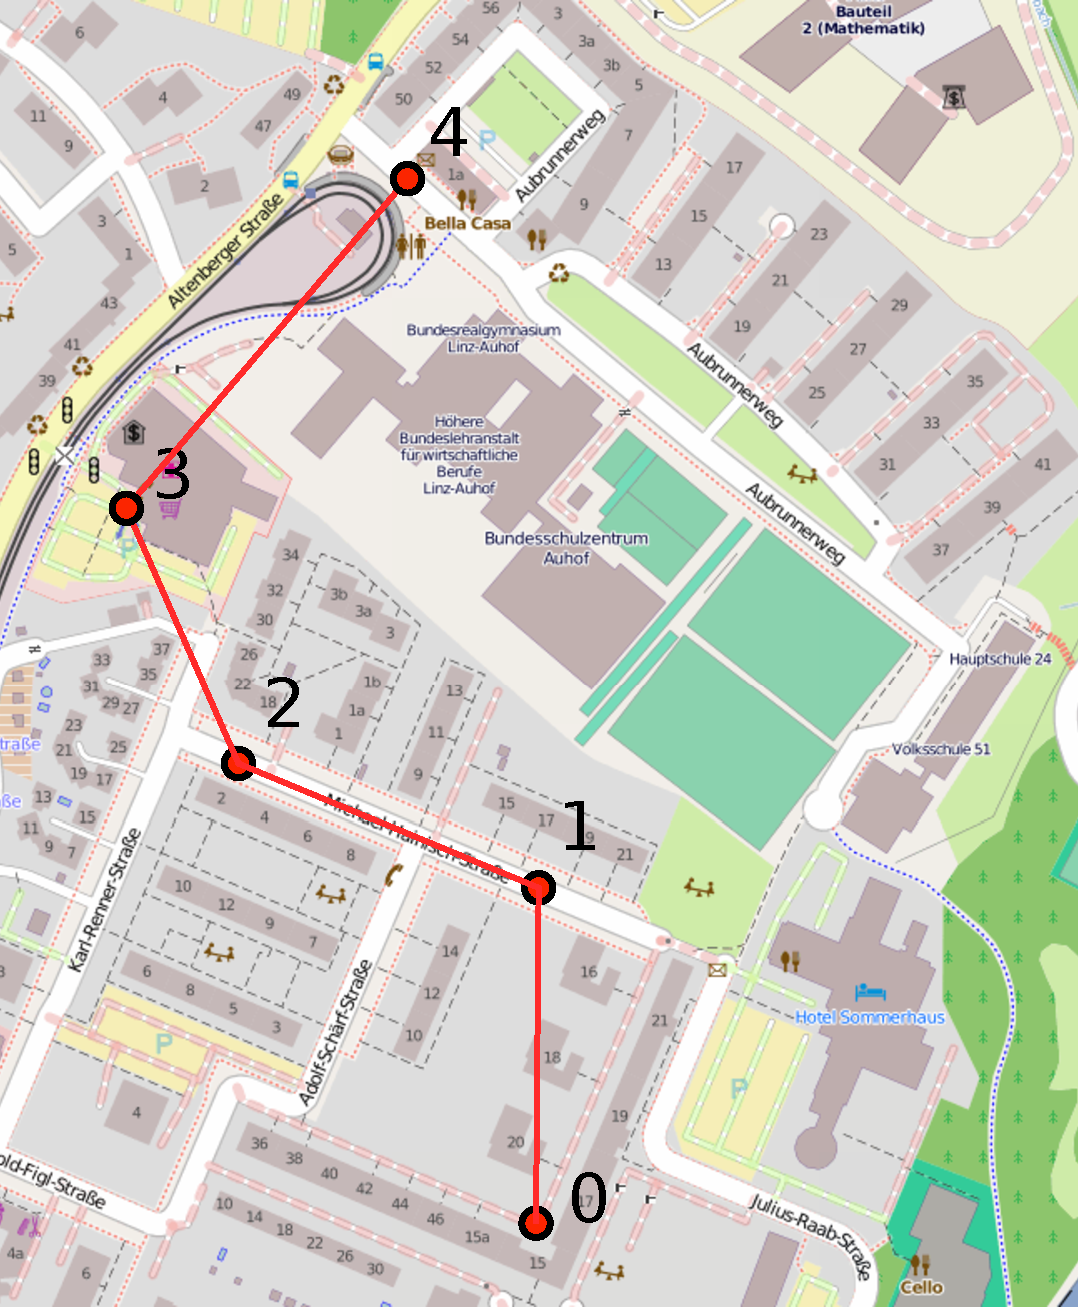
\includegraphics[width=0.31\textwidth]{img/gps}
   \label{img:gps-alchemist-navi}
  }
~
  \subfigure[Map-based navigation]{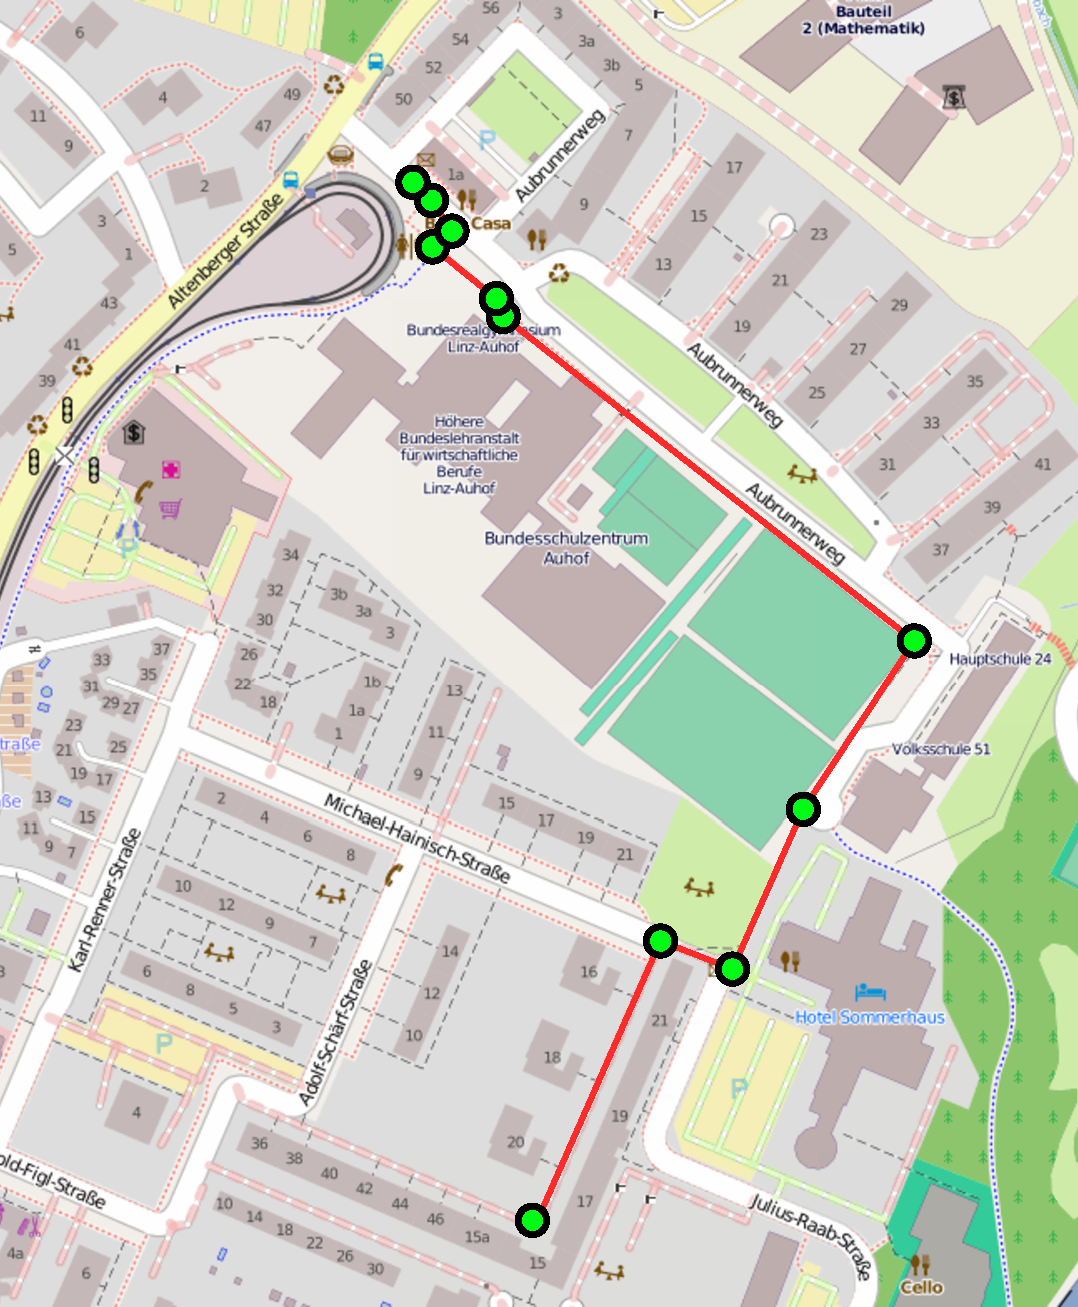
\includegraphics[width=0.31\textwidth]{img/map}
   \label{img:map-alchemist-navi}
  }
~
  \subfigure[Mixed mode]{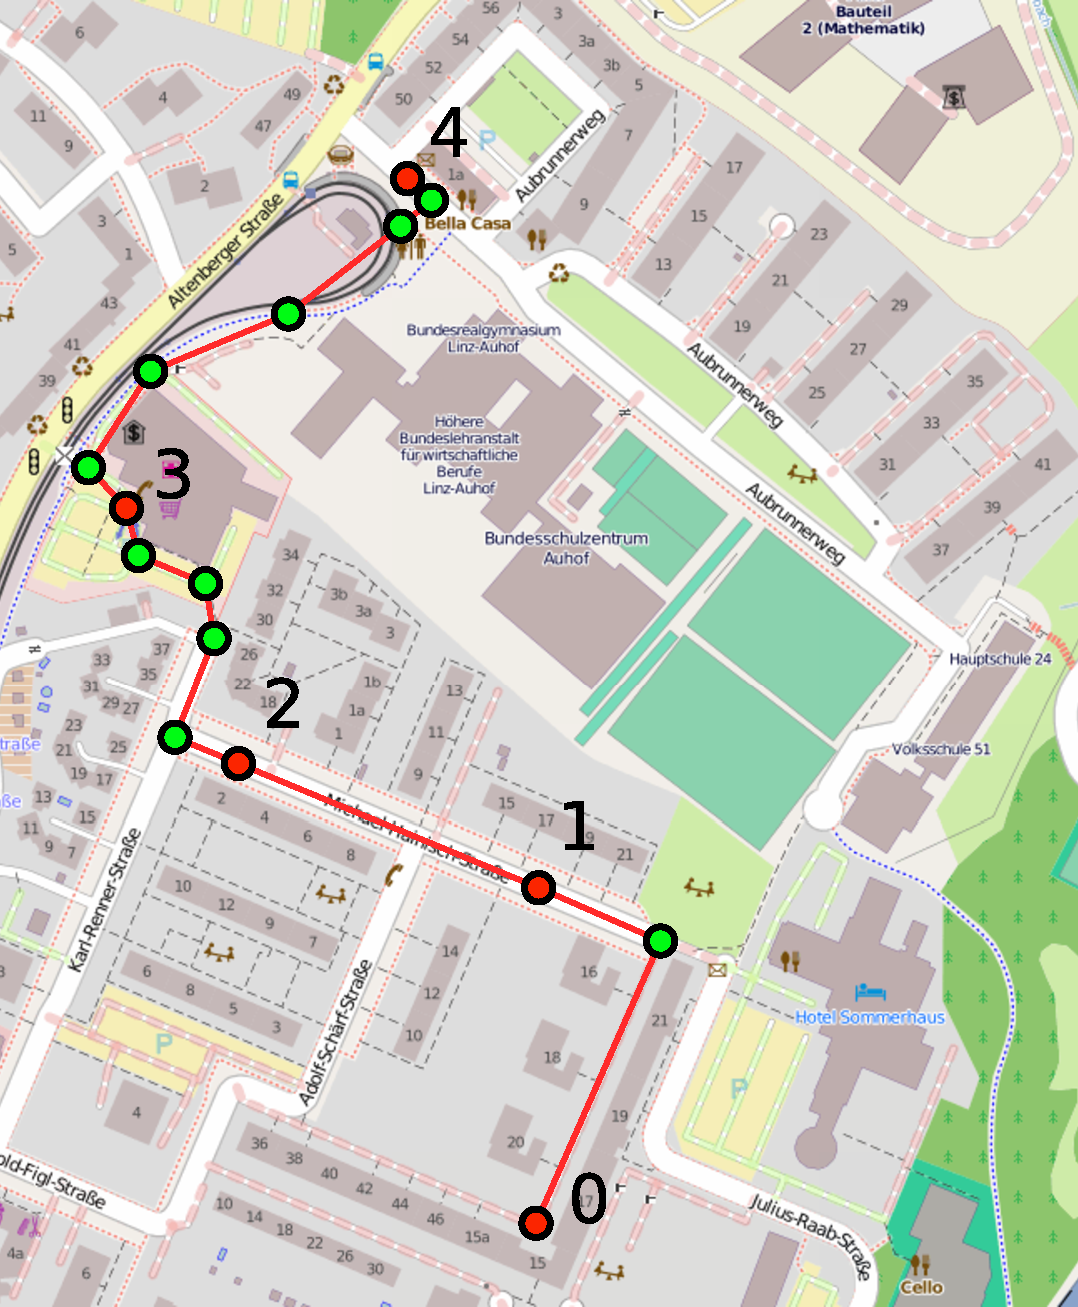
\includegraphics[width=0.31\textwidth]{img/mixed}
   \label{img:mixed-alchemist-navi}
  }
 \caption[Navigation modes in \alchemist{}]{Three snapshots showing the different navigation modes available in \alchemist{}. In \Cref{img:gps-alchemist-navi} there is a GPS trace consisting in four points. If not specified to behave otherwise, \alchemist{} computes the average speed between two points, and moves the node along a straight line with constant speed. This, depending on the precision of the trace, may generate paths that cross over buildings. In \Cref{img:map-alchemist-navi}, the route between the start and end point is computed using the built-in navigator. This could lead the nodes towards paths different from those described by the route. In \Cref{img:mixed-alchemist-navi}, the routing subsystem is used to refine the quality of the GPS traces: \alchemist{} will move the node with constant speed between the two points, using map based routing when necessary to improve precision between two consecutive trace points.}
 \label{img:traces-navigation}
\end{figure}

The second useful feature is the possibility to rely on the map data to compute routes, as in \Cref{img:map-alchemist-navi}.
%
\alchemist{} in fact ships with a module based on GraphHopper \footnote{\url{http://graphhopper.com/}} which provides the simulator the ability to compute routes between two points of the map.
%
This feature is mainly used to steer nodes correctly along the map, following the allowed ways.
%
It is possible to use such feature also specifying different types of vehicle.
%
Currently, pedestrians, bikes and cars are supported, and can be used together in the same simulation, and even within the same node (for e.g. simulating a pedestrian taking her car, driving and then walking again).
%
Another usage of this system is, for instance, the possibility to use the route distance or expected route time as data items when performing internal calculations, e.g. to compute a spatial gradient where the distance is not the classic euclidean distance but rather the distance computed by the routing subsystem.

The simulator also allows for loading GPS traces.
%
The traces must be in a personalised binary format, fortunately, however, this format is easy to generate.
%
In fact, it is just a Java object stream containing a List of ``IGPSPoints'', namely a simple structure with latitude, longitude and time.
%
A converter from JSON to such format is also available in the simulator distribution.
%
Just as the previously mentioned routing system, the GPS traces can be used to move nodes along the scenario, reproducing existing paths, as in \Cref{img:gps-alchemist-navi}.

It is also possible to use a combo of the two techniques: often, the GPS traces could be a bit rough with respect to desired grain of the simulation.
%
In these cases, the navigation subsystem can be used to compute the route between two GPS points, with the assumption that the user followed the paths allowed in the map.
%
In this way, it is possible to arbitrarily refine the grain of a GPS trace without the disadvantage deriving from a simpler interpolation, namely the possible transit over physical obstacles.
%
Such mixed navigation mode is depicted in \Cref{img:mixed-alchemist-navi}.

Obviously, it would be rather hard to understand what is going on on the simulation without proper rendering support.
%
In this sense, \alchemist{} automatically detects when a real-world environment is being used, and renders a map relying on MapsForge \footnote{\url{https://code.google.com/p/mapsforge/}}.



\chapter{Chemical meta-model}

% TODO: description, mi sa che tocca farla a mano...

\section{Example scenario: Morphogenesis}

As example to test the power of a chemical stochastic simulator enriched a more general model, we propose a case study on morphogenesis.
%
Development of multicellular organisms begins with a single cell -- the fertilised egg, or zygote.
%
The egg cell is always asymmetric, \emph{i.e.}, the distribution of maternal proteins inside the cell is not uniform.
%
After fertilisation it divides mitotically to produce all the cells of the body. 
%
The resulting blob of cells starts the process of differentiation which is initially caused by the presence of \emph{maternal factors} located in specific areas of the organism's egg.
%
The ordered spatial organisation of this diversity is then caused by the interactions among cells. These can be direct or mediated by specific diffusing proteins called \emph{morphogens}. 
%
After that, tissues have been created, and the formation of organs begins so as to originate the final shape of the organism \cite{alberts, gilbert2006-devbio}. 

The main issues of Developmental Biology, nowadays only partially solved, are:
\begin{itemize}
 \item which are the processes and the genetic mechanisms that control cellular (or nuclear) duplication;
 \item which are the processes and the genetic mechanisms by which cells differentiate;
 \item how it is possible that cellular differentiation is spatially organised.
\end{itemize}

It is clear that the macroscopic emergent results of pattern and shape formation originates from the microscopic mechanisms of intra-cellular reactions and environmental morphogen diffusion.
%
But how these mechanisms coordinate is still under investigation through experimental techniques and theoretical models.

%%%%% Drosophila models
A well known example of multicellular development is given by \emph{Drosophila Melanogaster}, whose spatial organisation results in the segmented pattern of gene expression shown in  \Cref{fig:drosophila}. 
%
To show the spatial-temporal evolution of the pattern, the organism has been object of several modelling attempts, most of which focus their investigation in gene interactions and protein diffusion mechanisms, bounding the window of analysis at a period of development that does not massively involve nuclear or cellular divisions. 
%
To cite few of them, in \cite{reinitz95} the change of protein concentration is modelled as an Ordinary Differential Equation depending on the process of gene regulation, diffusion over a  discretised space and decay.  Mitosis are also modelled as a synchronous  atomic process that suspends the synthesis of protein and causes a doubled number of cell nuclei.
%
In \cite{gursky04} it is presented a continuous mathematical model based on a set of coupled non linear reaction-diffusion Partial Differential Equations  that describe how protein concentrations change over time and space as a result of the mechanisms of protein synthesis and degradation, gene inhibition and activation, protein diffusion. They replace embryo's cellular structure with a continuum and do not model nuclear divisions. 
%
%Simulations are performed from cl. cyc 11 to 14.
%
In \cite{montagna-cs2bio10} it is described a stochastic and discrete version of  \cite{gursky04} based on a set of interacting compartments inside which chemical reactions implementing the gene regulatory network can occur. It does not count for changes in the network topology due to compartment movement and mitosis.
%
These models run over a simulation window that start from cleavage cycle 11 to cleavage cycle 14.
%
In \cite{LeccaJIB2010} the gradient formation of the Drosophila \emph{bicoid} protein, mainly caused by the morphogen diffusion, is simulated with an innovative stochastic model of reaction-diffusion systems implemented into a Gillespie-like stochastic simulation algorithm. They do not model neither gene interactions nor cellular / nuclear divisions.
%

To capture a bigger window of embryo development we built on top of \alchemist{}'s chemical meta-model a model of \emph{Drosophila} development so as to capture  both nuclear division and molecular processes such as  morphogen diffusion and gene regulatory networks.

\subsection{Development of Drosophila Melanogaster}

\begin{figure}
\centering
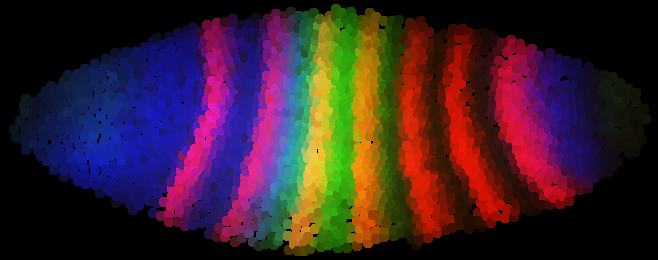
\includegraphics[width=0.99\textwidth]{img/drosophila}
\caption[Drosophila Melanogaster embryo at the cleavage cycle 14A temporal class 8]{The pair-rule gene  \emph{even-skipped} (red) together with \emph{hb} (blue) and \emph{Kr} (green) in \emph{Drosophila} embryo at the cleavage cycle 14A temporal class 8. Reconstructed image from \cite{flyex2009}. Embryo name: ba3. }
\label{fig:drosophila}       % Give a unique label
\end{figure}

\emph{Drosophila} is one of the best known multicellular organism. 
%
The egg of  \emph{Drosophila} is already polarised by differently localised mRNA molecules which are called \emph{maternal effects}. 
%
The early nuclear divisions are synchronous and fast (about every 8 minutes): the first nine divisions generate a set of nuclei forming the \emph{syncytial blastoderm}. All the dividing nuclei share a common cytoplasm, and material can diffuse throughout the embryo. 
%
After other four nuclear divisions, during the fourteenth nuclear division, plasma membranes grow to enclose each nucleus, converting the syncytial blastoderm into a \emph{cellular blastoderm} consisting of about 6000 separate cells.  
%
After the first ten divisions the time required to complete each of the next four divisions becomes progressively longer: cycle 13 takes for instance 25 minutes. During cycle 14 cells conclude their mitosis in rather different time: some cells take 75 minutes, other 175 minutes to complete this cycle. The rate of division is then constant in the first hours of development (9.05 $min^{-1}$), then decreases until a low value (0.2 $min^{-1}$).
%
The transcription of RNA massively begins during cleavage cycle 14 so that the embryo enters in the mid-blastula transition.
%
\begin{figure}
\centering{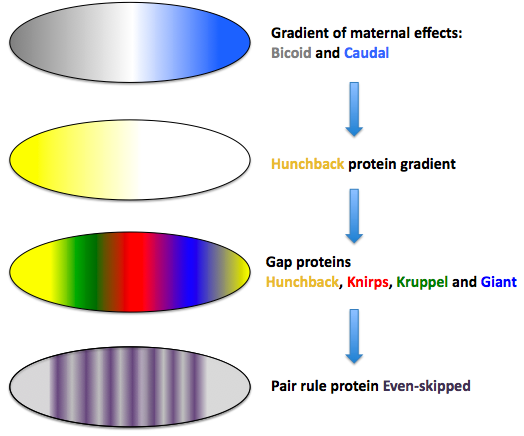
\includegraphics[width=0.99\textwidth]{img/drosi}}
\caption{Hierarchy of genes establishing the anterior-posterior body plan}
\label{fig:anterpostpattern}
\end{figure}

\noindent The studies on the genetics at the basis of the segmentation in the anterior-posterior body plan identified a hierarchy of genes that controls segment determination: maternal effects, gap genes, pair-rule genes and segment polarity genes. In \Cref{fig:anterpostpattern} an illustrative subset of this hierarchy is shown ---in the images of this chapter we hereafter refer at the anterior pole as their left side, and the posterior as their right side. 
%
Maternal effect genes are the building blocks of the anterior-posterior pattern. The most important are \emph{bicoid} (bcd)  -- forming an anterior-to-posterior gradient -- and \emph{caudal} (cad)---forming a posterior-to anterior gradient. 
%
The mRNAs of such genes are placed in different regions of the egg and initiate the hierarchy of transcription, driving the expression of \emph{gap genes}, which are the first zygotic genes to be expressed. The first is \emph{hunchback} (hb), that appears early in the embryo development such that sometimes is classified among maternal genes. The basic others are \emph{Kr\"{u}ppel} (Kr), \emph{knirps} (kni) and \emph{giant} (gt).
%
These genes are expressed in specific and partially overlapping domains. 
%
Differing combinations and concentrations of the gap gene proteins then regulate the expression of downstream targets, \emph{i.e.}, the \emph{pair-rule genes}, which divide the embryo into a striped pattern of seven segments. The most important pair-rule genes are  \emph{even-skipped} (eve) and  \emph{fushi-tarazu} (ftz).
%
The pair-rule gene proteins activate the transcription of the \emph{segment polarity genes},  whose protein products specify 14 parasegments that are closely related to the final anatomical segments \cite{alberts}.

We developed a model that reproduce the process of \emph{Drosophila} development from the fertilised egg until the pattern formation of the \emph{gap genes} during cleavage cycle 14.
%
The whole embryo is modelled as a big cell where nuclei grow and move over a 2D continuous environment filled with diffusing proteins.
%
The mechanisms we explicitly model and we reproduce with simulation are:
\begin{itemize}
 \item nuclear divisions;
 \item nuclear migration;
 \item morphogen diffusion;
 \item gene interactions.
\end{itemize}

We model the process of nuclear divisions as a single chemical like reaction, whose precondition is given by the maximum number of other nuclei in the neighbourhood and whose product is a new nucleus. 
%
The new nucleus is created close to the dividing one in a casual direction and owns half of its molecular content.
%
The rate of nuclear division is determined according to the rate observed in the real system.
%
Since experimental data show a certain synchronisation among dividing cells, this phenomena has been modelled through a non-Markovian reaction, relying instead on a ``drifting'' Dirac Comb, namely on a distribution whose events happen every increasing time interval.

Movement of nuclei is based on biomechanical forces of repulsion among neighbouring nuclei. They are in fact constrained to remain within the membrane-delimited area so as to filling pretty homogeneously the available space.
%
If two nuclei are closer than a distance given as a parameter, a new position for them is computed. The nearer two nuclei are, the stronger is the repulsion.

We support diffusion from / to nuclei and inside the environment along the $x$ and $y$ axis.
%
For this purpose environment is discretised into a grid of locations.
%
Molecules move from one nucleus into a neighbour location of the environment picked up probabilistically among the whole neighbourhood, or, the other way round, from one location of the environment into a neighbouring nucleus.
%
Diffusion among locations of the environment follows the same law, implementing a Brownian motion.

In \Cref{fig:genenetwork} it is shown the network of interactions among maternal effectors and gap genes we considered. As in \cite{perkins-compbio06}, an other gap gene, \emph{tailess} (tll), also  appears as input of the network whose regulation is not clear and we do not represent in the model. 

\begin{figure}
\centering{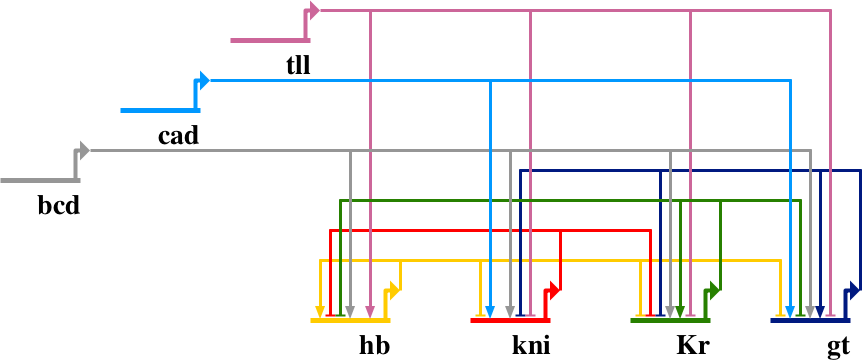
\includegraphics[width=0.99\textwidth]{img/network}}
\caption[Gene regulatory relationships as in the model presented in \cite{perkins-compbio06,RiveraPomar,gursky04}]{Gene regulatory relationships as in the model presented in \cite{perkins-compbio06,RiveraPomar,gursky04}. The diagram is realised with BioTapestry \cite{biotapestry-2009}. The type of link is pointed out by its shape: links with arrowhead are enhancers, while the repressor links have a foot.}
\label{fig:genenetwork}
\end{figure}

\subsection{Simulation in \alchemist{}}

Simulations results are shown in \Cref{fig:simres}. They are evaluated observing the time evolution of the compartment number and of the gene expression pattern. 
%
The time evolution of cells number is compared with data we have from literature and described above.
%
Simulations results for gap genes expression are evaluated according to experimental data available online in the FlyEx database \cite{database-2008}\footnote{\texttt{http://urchin.spbcas.ru/flyex/} -- last visited on December 2014} and reported in \Cref{fig:expdata}. They provide only qualitative information and their evaluation is  based on the expression area of the different genes.

The snapshots  in \Cref{fig:simres} show one side of the embryo along the anterior-posterior (A-P) axis where almost half of the nuclei are located. The cell number is shown in the label on top of each snapshot. The horizontal axis represents the A-P position and  is labelled as \% of embryo length.

The first snapshot shows the initial condition with only one nucleus and the egg polarised by maternal effects localised in the extreme pole: \emph{bcd} on the left and \emph{cad} on the right.
%
During the first minutes of simulation only nuclear divisions occur so as to fill the whole maternal cell at the end of cleavage cycle 9 with around 250 nuclei (half of the total 500), as shown in the second snapshot. 
%
Finally in the third snapshot it is reproduced the expression pattern of the four gap genes, whose spatial organisation is compared with experimental data of \Cref{fig:expdata}. Cells are coloured  of yellow, red, blue and green if, in order, they express \emph{hb}, \emph{kni}, \emph{gt} and \emph{Kr}, and their size is proportional to the protein concentration.
%
Gene \emph{hb} is massively expressed in the anterior half of the embryo and a small segment appears in the extreme left: simulations correctly reproduce the main expression domain of \emph{hb} while, even if its expression is observable in the posterior pole, it does not form a clear segment.
%
Gene  \emph{kni} is mainly expressed between 60\% and 80\% of the embryo length, either in real embryo and in simulations,
%
as well as gene  \emph{Kr}, which is expressed between 40\% and 60\% of the A-P axis.
%
The expression of  \emph{gt} is finally observable between 10\% and 30\% and 80\% and 90\%. The qualitative results presented here are not sufficient for observing the expression in the anterior half of the embryo as soon as it totally overlaps the \emph{hb} expression, while the posterior segment clearly appears.
%
%Beside the anterior expression of \emph{gt}, which is still subject of investigation, the simulation correctly reproduces the real embryo pattern.


\begin{figure}
\centering{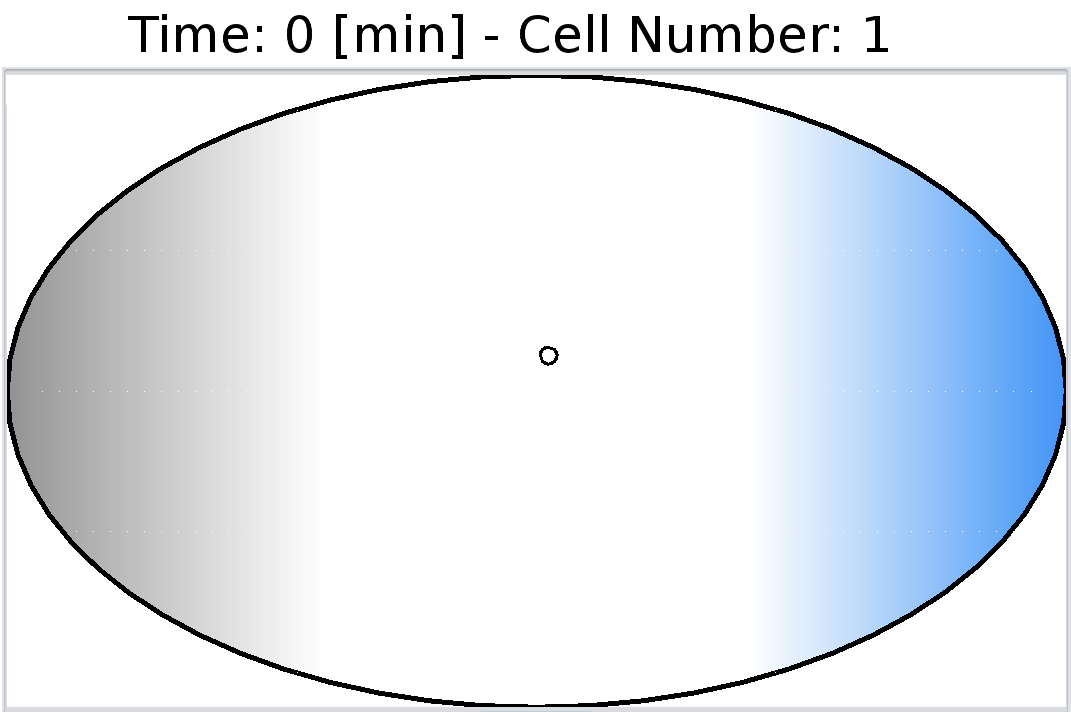
\includegraphics[width=0.6\textwidth]{img/simu_time0}}
\centering{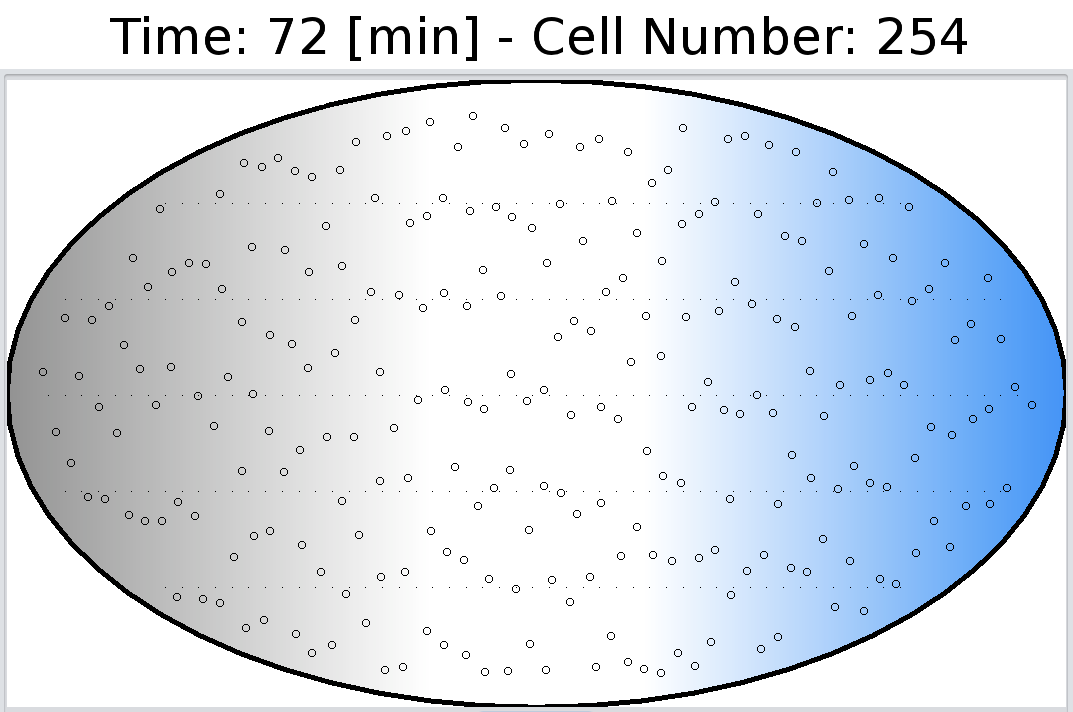
\includegraphics[width=0.6\textwidth]{img/simu_time72}}
\centering{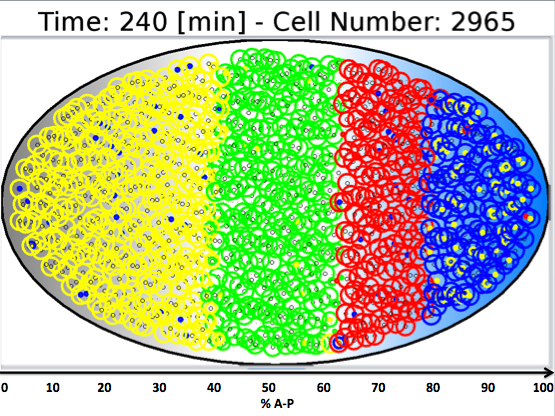
\includegraphics[width=0.6\textwidth]{img/simu_time240}}
\caption[Simulation results for the Drosophila development]{Simulation results for the four gap genes \emph{hb} (yellow), \emph{kni} (red), \emph{gt} (blue), \emph{Kr} (green) at a simulation time equivalent to the eighth time step of cleavage cycle 14A}
\label{fig:simres}
\end{figure}

\begin{figure}
\centering{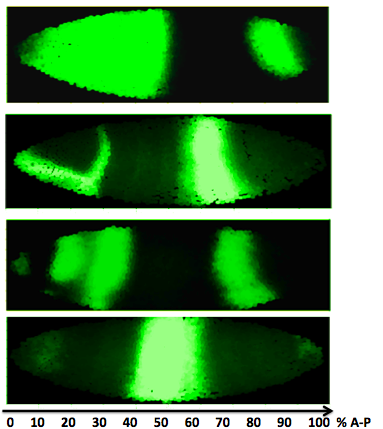
\includegraphics[width=0.99\textwidth]{img/expdata}}
\caption[Drosophila experimental data]{The experimental data for the expression of (from the top) \emph{hb}, \emph{kni}, \emph{gt}, \emph{Kr} at the eighth time step of cleavage cycle 14A  \cite{database-2008}, \copyright Maria Samsonova and John Reinitz}
\label{fig:expdata}
\end{figure}


\chapter{SAPERE meta-model}

\part{Methods and patterns for self-organisation}

\chapter{A process algebra for SAPERE}
\label{sapere-process-algebra}
In this\levelText{}we present a possible formalisation of the SAPERE concepts, in terms of a model whose evolution is specifyied by means of a process algebra.
%
Not only does this formalisation act as a non-ambiguous description, it is also an executable specification and can hence serve as ground for developing simulations of self-organisation mechanisms and for deriving formal proofs of behavioural properties, like self-stabilisation \cite{V-SCW2013}.
%
Few works attempted at a process algebraic formalisation of self-organisation \cite{VPB-COORD2012,VDB-FOCLASA-CIC2013}, developing on top of well-known works on coordination and spatial computing \cite{zavattaro2,proto}.
%
However, the one presented here is -- to the best of our knowledge -- the first process algebra of self-organising multiagent systems capturing the clear separation of agent behaviour and self-organised interactions, hence effectively expressing the behaviour of large-scale and situated pervasive computing scenarios.

\section{Model}

We now detail a possible coordination model of pervasive ecosystems.
%
It is important to note upfront that the presented coordination model can be instantiated in different ways, depending on the application at hand and on technological aspects: This affects the concrete structure of data, which is an issue orthogonal to the above aspects.
%
A similar abstraction is rather common in the description of space-based coordination models, which often represent tuples as simple atomic elements \cite{zavattaro}.

\subsection{LSAs}

LSAs have a unique, system-wide identifier (LSA-id), needed to support a notion of identity that is key both to uniquely identify the agent that injected an LSA and to properly support a bonding mechanism based on reference and not on value/copy. We refer to the content of an LSA as its \emph{description}, which includes all the information the agent wants to manifest to the ecosystem.
%
Several concrete approaches to the structure of an LSA description can be taken.
%
For the sake of exemplification, following the work in \cite{SemanticSapereIGI2012,sapereecolaws-sac2012,SemMatchingSAC2013} we  take a semantic approach based on Resource Description Framework (RDF) representation \cite{manola2004primer}, in which an LSA is a set of multi-valued properties, or equivalently, a set of triples (subject, predicate, object) of an LSA-id, the property name, and the assigned value, expressed as literals (strings) or URIs (terms qualified by universally-accessible namespaces, to which an ontological interpretation can be given \cite{ranganathan2004ontologies}).
%
An example LSA advertising an exhibition in a smartcity, to be diffused around, would be: 

{\begin{Verbatim}[samepage=true,frame=single,commandchars=\\\{\}]
[ app:type = app:poi, app:event = app:exhibition,
  app:artist = "caravaggio" "michelangelo", ...]
\end{Verbatim}
}

\noindent URI \texttt{app:artist} represents a property name, assigned to the literal values \mbox{\texttt{"caravaggio"}} and \mbox{\texttt{"michelangelo"}}. Alternatively, a value can be an URI again, like \texttt{app:exhibition} that is associated with \texttt{app:event}. Namespace \texttt{app} is used here to refer to a publicly accessible ontology supporting semantic reasoning on top of those properties and values \cite{SemMatchingSAC2013}.

\subsection{Agent primitives}\label{s:agent}

Standard tuple-based coordination models allow agents to insert, read, and remove any tuple (by primitives \texttt{out}, \texttt{rd} and \texttt{in}) without specific access control constraints---although some models explore their orthogonal adoption, like SecSpaces \cite{GorrieriLZ06} and coordination contexts \cite{J-ORV-AAECC2005,RVO-ATAI2004}.
%
The model we present is profoundly different, mainly due to the chemical metaphor of bonding and the manifestation/observation approach it entails, which guarantees a better modularisation and control of accesses of agent behaviour---see a deeper discussion in Section 6.
%
In particular, the following 4 primitives are provided:

\begin{itemize}
 \item \texttt{new(Description):Id} | This operation relates to creating a new agent manifestation in the system. It takes a description (namely, a property-value association), and correspondingly generates a new LSA and inserts it into the local LSA-space. A new identifier, associated to that LSA, is then automatically created and returned to the agent: it will be used to perform subsequent operations on the LSA. That agent will be called the \emph{owner} of the LSA.
 
 \item \texttt{update(Id,Update)} | This operation relates to the (continuous) manifestation of agent state. It takes the identifier of an LSA owned by the current agent, and the specification of an update to its current description (typically, property-value re-assignments), and it updates the description of such an LSA. Note that only an LSA owner can modify it. 
 
 \item \texttt{observe(Id,Query):Result} | This operation relates to the  observation of an agent's context, namely, of some LSA residing in the same space but possibly belonging to some other agent. It takes the identifier of an owned LSA $l$ and a query, and searches for an LSA bonded to $l$ that provides a valid result to the query. If one is found (nondeterministically), the query result is returned, typically in the form of a set of variable-value associations. The semantics of bonding is orthogonal to that of agent primitives: it is dictated by the structure of a specific bonding eco-law, as described in the following. %Operation \texttt{observe} fails if no proper result is found.
 
 \item \texttt{remove(Id)} | Finally, this operation relates to the stopping manifestation. It takes the identifier of an owned LSA, which will then be removed from the local LSA-space.
 
\end{itemize}

\subsection{Eco-laws}\label{s:ecolaws}

Without any additional mechanism, the behaviour of an agent would be isolated from those of others.
%
Following the ecosystem metaphor, we hence introduce a limited set of eco-laws (playing the role of ``the laws of nature''), with the role of evolving the population of tuples over time in a way that supports agent-to-agent interaction both within the same locality, and globally by means of self-organisation.
%
This is achieved in terms of $5$ eco-laws, two dealing with local agent-to-agent interaction by the bonding (and debonding) mechanism, and the other $3$ (diffusion, aggregation and decay) supporting the mechanisms needed to create self-organising distributed structures of LSAs \cite{FDMVA-NACO2012}.
%
As already mentioned, our description of eco-laws abstracts from the actual structure of LSAs and from the details of pattern matching, which we consider as orthogonal application- and infrastructure-dependent aspects.

\begin{itemize}

 \item \texttt{bonding}  | This is the eco-law regulating the creation of bonds. A bond is an asymmetric reference between two LSAs residing in the same space. As already described, the existence of a bond between LSA $X$ and $Y$ means that the owner of $X$ can observe the structure of $Y$ via the \texttt{observe} primitive. This eco-law makes sure that a bond between two LSAs exists as long as their description matches according to an infrastructure-specific matching function. In the typical case, a bond is created between an LSA providing a (possibly semantic) query and an LSA positively replying to the query. By denoting with ``$\rightsquigarrow Y$'' the existence of a bond to $Y$, this eco-law has the chemical-like structure\footnote{Symbol ``$+$'' is used as separator as in chemical laws.}:
 
 \[X + Y \rightarrow X^{\rightsquigarrow Y} + Y\]
 
 \item \texttt{debonding}  | This eco-law is dual to the previous one, and regulates destruction of a bond between $X$ and $Y$ provided the conditions for the bond are no longer satisfied, namely, when either $X$ or $Y$ are removed or changed. It has the structure:
 
 \[X^{\rightsquigarrow Y} + Y \rightarrow X + Y\]
 
 \item \texttt{diffusion} | The diffusion eco-law is used to create a clone of an LSA to be shipped to all neighbours of the current node. This eco-law applies to an LSA $X$ that has a particular structure (typically, given property-value associations). The LSA $X'$ accordingly created has a new identifier along with an updated value of some special properties that can keep track of the increased distance from the source (the notion of distance can be extended to consider advanced forms of context-dependency as described in \cite{SemMatchingSAC2013}). Note that such a new LSA has no owner: it is typically used to create a distributed structure of LSAs representing the global outcome of a single LSA initially created by an agent. By denoting with notation $\overrightarrow{X'}$, an LSA $X'$ to be spread to neighbours, we can express the structure of this eco-law as:
 
 \[X \rightarrow X + \overrightarrow{X'}\]
 
 \item \texttt{aggregation} | As the diffusion eco-law keeps creating copies of an LSA that are shipped to neighbours, the aggregation eco-law has the goal of addressing the implied multiplicity---ensuring that a single version of an LSA coming from the same source is present in a node. In particular, this eco-law takes two compatible LSAs $X$ and $Y$ (typically, two coming from the same ``source'' LSA after an iterative diffusion process) and aggregates them into a single one $X'$ exploiting a suitable order-independent aggregation function. It has the structure:
 
 \[X + Y \rightarrow X'\]
 
 \item \texttt{decay} | In order to provide a temporal cleanup mechanism, useful to refresh information and the shape of spatial structures, a decay eco-law is also considered, which takes an LSA $X$ and erases it as soon as a given condition on its content holds. Denoting $\epsilon$ as the empty set of LSAs, it has the structure:
 
 \[X \rightarrow \epsilon\]
 
\end{itemize}

\section{Formalisation}

In this\levelText{}we provide a formalisation of the proposed coordination model as informally presented in previous section. We adopt the style that has now became a standard after a series of previous works---starting from the work of Zavattaro et.al. \cite{zavattaro}, as surveyed in \cite{VO-FI2006}, and more recently including, e.g., \cite{VPB-COORD2012,TerepetaNN12,BortolussiLM13,MassinkL12,LaneseBF13}.
%
Namely, this is presented in the form of a process algebra, in which a system state is conceived as a ``soup'' (or networked set of soups) where agents and LSAs float: subjective coordination is realised by agents performing coordination primitives amounting to interactions with the local space (producing/consuming/modifying LSAs), while objective coordination is realised by eco-laws executing as rules continuously manipulating the space on top \cite{biochemicalTupleSpaces,tucson-aamas99,RicciOD02}.
%
This approach has been shown to elegantly express the semantics of the various constructs in an orthogonal way, that is, one rule of operational semantics per coordination primitive (and this will indeed be the case for our formalisation as well). 
%
Additionally, using process algebras paves the way for advanced analysis similarly to what developed in related approaches, including mathematical proofs of behavioural properties \cite{V-SCW2013}, simulation \cite{sapereecolaws-sac2012,DeNicolaLM05}, and observational equivalence \cite{LaneseBF13}.
%
%Critically, this is the first process algebra of coordinating agents that is able to express self-organisation of large-scale situated systems.

\begin{figure}[!t]{
 \framebox[1\textwidth]{$
\begin{array}{l}
~\\[-10pt]
\begin{array}{rl}
%
%\multicolumn{2}{l}{\hspace{-20pt}\textrm{Metavariables:}}\\
\sSI & \textrm{Node identifier}\\
\sId,\sIdB & \textrm{LSA identifier}\\
\sVr & \textrm{Identifier variable}\\
\sDe,\sDeB & \textrm{LSA description}\\
\sDE & \textrm{Update specification}\\
%\sLb & \textrm{Action label}\\
%\snew & \textrm{A freshly generated identifier}\\
\cList{v} & \textrm{A meta-variable over set of elements $\{v_1,\ldots,v_n\}$}
\end{array}\end{array}$}} \caption[Meta-variables for a SAPERE algebra]{Meta-variables} \label{fig:meta}
\end{figure}


\subsection{Syntax}

We let meta-variable $\sSI$ range over node (or device) identifiers, $\sId,\sIdB$ over LSA identifiers, $\sVr$ over variables to be eventually substituted by those identifiers, $\sDe,\sDeB$ over LSA descriptions, and $\sDE$ over update specifications. Given any of those meta-variables, we use the overline notation to indicate a meta-variable over sets of elements (e.g., $\cList{\sId}$ is a meta-variable over sets of LSA identifiers)---and similarly for the others. \Cref{fig:meta}  recalls these meta-variables in tabular form for the reader's convenience. Notation $|\cList{\sId}|$ is used to extract the number of elements in $\cList{\sId}$.

The syntax of the calculus is reported in \Cref{fig:syntax}. A system configuration $\sCf$ is a multiset composition (by operator $|$) of spaces of the form $\cSpace{\sSp}{\sSI}$ ($\sSp$ is the content and $\sSI$ the identifier), and neighbourhood relationships $\cNeigh{\sSI}{\cList{\sSI}}$, meaning $\sSI$ has the neighbourhood $\cList{\sSI}$.
%
A space (content) $\sSp$ is itself a multiset composition of agents $\cAgent{\cList{\sId}}{\sAg}$ (with behaviour $\sAg$ and owning LSAs with identifiers $\cList{\sId}$), LSAs $\cLSA{\sId}{\sDe}$ (with identifier $\sId$ and a description $\sDe$), LSAs to be spread to  neighbours $\cLSA{\sStar}{\sDe}$ and bonds $\cBond{\sId}{\sIdB}$ (from $\sId$ to $\sIdB$).
%
Agent behaviour $\sAg$ can be of four kinds:
\begin{enumerate}
 \item $0$ is the empty agent;
 \item $\sAc \oSeq \sAg$ is the agent executing action $\sAc$ and then the continuation $\sAg$;
 \item $\sAg\oOr\sAgB$ is a try-catch construct (execute $\sAg$, and when/if a failure occurs, $\sAgB$ is executed);
 \item $\cRecR{\sAg}{\sAgB}$ is iterative (infinite) execution of $\sAg$ preceded by execution of current iteration $\sAgB$.
\end{enumerate}
%
Note that in the iteration construct the appendix $\sAgB$ is not present in the surface syntax: it is initially set to $0$ and will dynamically keep track of the state of current iteration.

Actions correspond to the $4$ coordination primitives described in previous section: $\cNew{\sVr}{\sDE}$ creates a new LSA with description defined by specification $\sDE$, and causing substitutiion of $\sVr$ with the LSA identifier; $\cUpd{\sTr}{\sDE}$ updates the LSA with term identifier $\sTr$ by specification $\sDE$; $\cObs{\sTr}{\sDE}$ observes an LSA bond to $\sTr$ using $\sDE$ as a query; and finally $\cRem{\sTr}$ removes LSA with identifier $\sTr$. In particular note that as soon as they are executed, the latter three constructs should have term identifier $\sTr$ be bound to an actual identifier $\sId$.

A congruence relation is also introduced in \Cref{fig:congruence}, which equates terms that have to be considered syntactically equivalent. The first two lines state that parallel composition operator is actually a multiset one; the third line defines properties of try-catch (if the left-hand side is over, the whole agent process is over) and iteration (iterating the empty process gives the empty process, and when current iteration is over we spawn a new one).

\begin{figure}{
 \framebox[1\textwidth]{$
\begin{array}{l}
~\\[-10pt]
\begin{array}{@{\hspace{-0.08cm}}rcl@{\hspace{0.5cm}}r}
%
\sCf & \BNFp &  0 \BNFor
		\cSpace{\sSp}{\sSI} \BNFor
		\cNeigh{\sSI}{\cList{\sSI}} \BNFor
		(\sCf \oPar \sCf)
		&   {\footnotesize \mbox{Configuration}} \\[2pt]
\sSp & \BNFp &  0 \BNFor 
		\cAgent{\cList{\sId}}{\sAg} \BNFor
		\cLSA{\sId}{\sDe} \BNFor
		\cLSA{\sStar}{\sDe} \BNFor
		\cBond{\sId}{\sIdB} \BNFor
		(\sSp \oCPar \sSp)
		&   {\footnotesize \mbox{Space}} \\[2pt]
\sAg,\sAgB & \BNFp &  0 \BNFor 
		%\sAc \BNFor
		\sAc \oSeq \sAg \BNFor
		\sAg\oOr\sAgB \BNFor
		\cRecR{\sAg}{\sAgB}
		&   {\footnotesize \mbox{Agent}} \\[2pt]
\sAc & \BNFp &  \cNew{\sVr}{\sDE} \BNFor
		\cUpd{\sTr}{\sDE} \BNFor
		\cObs{\sTr}{\sDE} \BNFor
		\cRem{\sTr}
		& {\footnotesize \mbox{Action}} \\[2pt]
\sTr & \BNFp &  \sId \BNFor
		\sVr
		& {\footnotesize \mbox{Term}} \\[2pt]
%
\end{array}
\end{array}$}} \caption[Syntax of a SAPERE algebra]{Syntax} \label{fig:syntax}
\end{figure}



\begin{figure}{
 \framebox[1\textwidth]{$
\begin{array}{l}
~\\[-10pt]
\begin{array}{c}
%
\sCf\oPar 0 \equiv \sCf\qquad \sCf\oPar \sCf' \equiv \sCf'\oPar \sCf \qquad (\sCf\oPar \sCf')\oPar\sCf'' \equiv \sCf\oPar (\sCf'\oPar\sCf'')\\
%
\sSp\oCPar 0 \equiv \sSp\qquad \sSp\oCPar \sSp' \equiv \sSp'\oCPar \sSp \qquad (\sSp\oCPar \sSp')\oCPar\sSp'' \equiv \sSp\oCPar (\sSp'\oCPar\sSp'')\\
%
0\oOr\sAg \equiv 0 \qquad %(\sAg\oOr \sAg')\oOr\sAg'' \equiv \sAg\oOr (\sAg'\oOr\sAg'') \equiv 
\cRecR{0}{\sAg}\equiv 0\qquad
\cRecR{\sAg}{0}\equiv \cRecR{\sAg}{\sAg}\\
%
%\cSpace{\sSp}{\sSI}\oPar\cSpace{\sSp'}{\sSI}\equiv \cSpace{\sSp\oCPar\sSp'}{\sSI} 
%\cBond{S}{S'}\oCPar\cBond{S}{S'}\equiv\cBond{S}{S'}\\
\end{array}\end{array}$}} \caption{Congruence table of a SAPERE algebra} \label{fig:congruence}
\end{figure}

\subsection{Semantics}


\begin{figure}{
 \framebox[\textwidth]{$
\begin{array}{l}
~\\[-10pt]
\begin{array}{rl}
%
\fFilt{\sDE}{\sDe}=\sDe' & \textrm{Description filtering function}\\
\fDiff(\sDe)=\sDe' & \textrm{Diffusion function}\\
\fAggr(\sDe,\sDeB)=\sDe' & \textrm{Aggregation function}\\
\fDecay(\sDe) & \textrm{Decay predicate}\\
\fBond(\sDe,\sDeB) & \textrm{Bond matching predicate}
\end{array}\end{array}$}} \caption[A process algebra for SAPERE: abstracted functions]{Abstracted functions} \label{fig:func}
\end{figure}


\begin{figure}{
 \framebox[\textwidth]{$
\begin{array}{l}
~\\[-10pt]
\begin{array}{rrcll}
%
\ccrule{CGR-C}{
    \sCf_0
    & \trn{\sLb} &
    \sCf_1
}{
    \sCf'_0\equiv\sCf_0	
    \myquad 
    \sCf'_0
    \trn{\sLb} 
    \sCf'_1	
    \myquad 
    \sCf'_1\equiv\sCf_1
}
%
\ccrule{NEST}{
    \sCf\oPar\cSpace{\sSp}{\sSI}
    & \trn{\sLb} &
    \sCf\oPar\cSpace{\sSp'}{\sSI}
}{
    \sSp
    \trn{\sLb}
    \sSp'
}
%
\ccrule{SHIP}{
    \sCf\oPar\cSpace{\cLSA{\sStar}{\sDe}}{\sSI} 
    & \trn{\lship{\cList{\sId}}} &
    \sCf\oPar\prod_i \cSpace{\cLSA{\sId_i}{\sDe}}{\sSI_i}
}{
    \cNeigh{\sSI}{\cList{\sSI}}\in S\myquad |\cList{\sSI}|=|\cList{\sId}|\myquad\textit{fresh}(\cList{\sId})
}
%
\end{array}\end{array}$}} \caption[A process algebra for SAPERE: architectural rules]{Rules modelling architectural aspects} \label{fig:congruence_rules}
\end{figure}



\begin{figure}{
 \framebox[1.02\textwidth]{$
\begin{array}{c}
~\\[-10pt]
\begin{array}{rrcll}
%
\crule{CGR}{
\sSp_0
    & \trn{\sLb} &
    \sSp_1
    
}{
    \sSp'_0\equiv\sSp_0	
    \myquad 
    \sSp'_0
    \trn{\sLb} 
    \sSp'_1	
    \myquad 
    \sSp'_1\equiv\sSp_1
}
%
\crule{TRY}{
    \sSp\oCPar\cAgent{\cList{\sId}}{(\sAg\oOr\sAgB)}
    & \trn{\sLb} & 
    \sSp'\oCPar\cAgent{\cList{\sId}'}{(\sAg'\oOr\sAgB)}\;
}{
    \sSp\oCPar\cAgent{\cList{\sId}}{\sAg}\trn{\sLb}
    \sSp'\oCPar\cAgent{\cList{\sId}'}{\sAg'}
}
%
\crule{CATCH}{
    \sSp\oCPar\cAgent{\cList{\sId}}{(\sAg\oOr\sAgB)}
    & \trn{\lexc} &
    \sSp\oCPar\cAgent{\cList{\sId}}{\sAgB}
}{
    \sSp\oCPar\cAgent{\cList{\sId}}{\sAg}\ntrn{}\myquad A\not\equiv 0
}
%
%
\crule{ITER}{
    \sSp\oCPar\cAgent{\cList{\sId}}{\cRecR{\sAg}{\sAgB}}
    & \trn{\sLb} &
    \sSp'\oCPar\cAgent{\cList{\sId}'}{\cRecR{\sAg}{\sAgB'}}
}{
    \sSp\oCPar\cAgent{\cList{\sId}}{\sAg}\trn{\sLb}
    \sSp'\oCPar\cAgent{\cList{\sId}'}{\sAgB'}

}
\end{array}\\[15pt]
\begin{array}{rrcll}
%
~\\[-10pt]\shortincrule{NEW}{
    \sSp\oCPar\cAgent{\cList{\sId}}{\cNew{\sVr}{\sDE}\oSeq\sAg}
    & \trn{\lnew{\sIdB}} &
    \sSp\oCPar\cLSA{\sIdB}{\fFilt{\sDE}{0}}
    \oCPar
    \cAgent{\sIdB,\cList{\sId}}{\fSubs{\sAg}{\sIdB}{\sVr}}\quad\textrm{if}~\textit{fresh}(m)
}
%
\shortincrule{UPD}{
    \sSp\oCPar\cLSA{\sId}{\sDe}
    \oCPar
    \cAgent{\sId,\cList{\sId}}{\cUpd{\sId}{\sDE}\oSeq\sAg}
    & \trn{\lupd} &
    \sSp\oCPar\cLSA{\sId}{\fFilt{\sDE}{\sDe}}
    \oCPar
    \cAgent{\sId,\cList{\sId}}{\sAg}
}
%
\shortincrule{OBS}{
    \sSp\oCPar\cLSA{\sIdB}{\sDe}
    \oCPar
    \cAgent{\sId,\cList{\sId}}{\cObs{\sId}{\sDE}\oSeq\sAg}
    & \trn{\lobs} &
    \sSp\oCPar\cLSA{\sIdB}{\sDe}
    \oCPar
    \cAgent{\sId,\cList{\sId}}{\sAg^{\textit{matcher}(\sDE,\sDe)}}
    \quad
    \textrm{if}~\cBond{\sId}{\sIdB}\in\sSp
}
%
\shortincrule{REM}{
    \sSp\oCPar\cLSA{\sId}{\sDe}
    \oCPar
    \cAgent{\sId,\cList{\sId}}{\cRem{\sId}\oSeq\sAg}
    & \trn{\lrem} &
    \sSp\oCPar\cAgent{\cList{\sId}}{\sAg}
}
\end{array}\end{array}$}} \caption[A process algebra for SAPERE: coordination primitives]{Rules modelling coordination primitives} \label{fig:agent_rules}
\end{figure}

\begin{figure}{
 \framebox[\textwidth]{$
\begin{array}{l}
~\\[-10pt]
\begin{array}{rrcl@{\hspace{0.5cm}}l}
%
\shortincrule{DIFF}{
    \sSp\oCPar\cLSA{\sId}{\sDe} 
    & \trn{\ldiff} &
    \sSp\oCPar\cLSA{\sId}{\sDe}\oCPar\cLSA{\sStar}{\fDiff(\sDe)}
}
%

\crule{AGR}{
    \sSp\oCPar\cLSA{\sId}{\sDe}\oCPar\cLSA{\sIdB}{\sDeB}
    & \trn{\lagr} &
    \sSp\oCPar\cLSA{\sId}{\fAggr(\sDe,\sDeB)}
}{
    \cAgent{\sIdB,\cList{\sId}}{\sAg}\notin \sSp
}
%
\crule{DEC}{
    \sSp\oCPar\cLSA{\sId}{\sDe}
    & \trn{\ldec} &
    \sSp
}{{\fDecay(\sDe)}\myquad\cAgent{\sId,\cList{\sId}}{\sAg}\notin \sSp}   
%
\crule{BND}{
    \sSp\oCPar\cLSA{\sId}{\sDe}\oCPar\cLSA{\sIdB}{\sDeB}
    & \trn{\lbond} &
    \sSp\oCPar\cLSA{\sId}{\sDe}\oCPar\cLSA{\sIdB}{\sDeB}\oCPar\cBond{\sId}{\sIdB}
}{\fBond(\sDe,\sDeB)\myquad \cBond{\sId}{\sIdB}\notin\sSp}
%
\crule{DBND}{
    \sSp\oCPar\cBond{\sId}{\sIdB}
    & \trn{\lubond} &
    \sSp
}{\sSp\ntrn{}\sSp\oCPar \cBond{\sId}{\sIdB}}
\end{array}\end{array}$}} \caption[A process algebra for SAPERE: eco-laws]{Rules modelling eco-laws} \label{fig:eco_laws}
\end{figure}

The semantics of the calculus is parametric in the functions shown in \Cref{fig:func}, which are to be concretised to make the model fully executable---as we will develop in next section.
%
The filtering function gives semantics to updates and queries over LSA descriptions as follows.
%
First of all, given an update specification $\sDE$ and an LSA description $\sDe$, then $\fFilt{\sDE}{\sDe}$ gives the description obtained by applying $\sDE$ to $\sDe$---this function is assumed to be total.
%
Second, $\sDE$ can be seen as a query: we say it matches a description $\sDe$ with result $\theta$ (a binding of variables) if $\fFilt{\sDE\sSB}{\sDe}=\sDe$, namely, when $\sDE\sSB$ is seen as an update, it would not affect $\sDe$---intuitively, e.g., an LSA of type $a$, matches with a query asking whether its type is $X$ (and gives reply $a$), if updating the type of that LSA to $a$ leaves it unchanged.
%
As a mere example in this\levelText{}assume $\sDE$ and $\sDe$ are both lists of single-value assignments $p = v$, and that filtering \mbox{$\fFilt{\sDE}{\sDe}$} applies all assignments of $\sDE$ to $\sDe$, such that \mbox{$\fFilt{(p=1,q=2)}{(q=3,r=4)}=(p=1,q=2,r=4)$}. Observe that update $(q=3,r=X)$, where $X$ is a variable, can be seen as a query which applied to $(q=3,r=4)$ yields $\theta=\{X/4\}$, in that \mbox{$\fFilt{(q=3,r=X)\{X/4\}}{(q=3,r=4)}=(q=3,r=4)$} as described above.

The other four functions in \Cref{fig:func} work with LSA descriptions, and define the data-related aspects of eco-laws as described in the following.

The operational semantics is defined as a transition system with judgement $\sCf\xrightarrow{}\sCf'$, meaning that system configuration $\sCf$ can move to $\sCf'$ by a transition.
%
The operational semantics is split in three parts: general congruence rules (\Cref{fig:congruence_rules}), rules defining agent behaviour (\Cref{fig:agent_rules}), and finally rules defining eco-laws (\Cref{fig:eco_laws}), described in turn.

In \Cref{fig:congruence_rules}, rule [CGR-C] is the standard rule making congruent configurations be considered equivalent, rule [NEST] allows one to recursively enter a space, and finally rule [SHIP] defines the broadcast semantics: when an LSA-to-be-spread $\cLSA{\sStar}{\sDe}$ occurs in a space, a copy of it is sent to all neighbours (by action $\lship{\cList{\sId}}$, where $\cList{\sId}$ is a set of externally provided freshly-generated identifiers)---note that we abuse the notation as in \cite{FJ}, writing $\cList{\sId}$ for $\sId_1,\ldots,\sId_k$ and similarly for $\cList{\sSI}$.

\Cref{fig:agent_rules} provides the rules defining the internal behaviour of spaces, affecting agent behaviour.
%
Rule [CGR] states congruence inside spaces similarly to what [CGR-C] does for system configurations.
%
Rule [TRY] handles successful operations inside a try-catch construct: simply, in that case the left-hand side of operator ``$:$'' is allowed to proceed.
%
Rule [CATCH] conversely handles a failure: when the left-hand side of operator ``$:$'' gets stuck (and is not empty), we simply allow the part on right (the handler) to carry on.
%
Rule [ITER] handles the semantics of iteration: it simply allows the appendix to carry on---when it becomes $0$ a new iteration will be spawn by the congruence relation as discussed above.

The subsequent $4$ rules handle the $4$ coordination primitives of the model.
%
Rule [NEW] create a new LSA with fresh identifier $\sId$: such an LSA gets created with description $\fFilt{\sDE}{0}$ (namely, as specified in the argument of operation \texttt{new}), $\sId$ is added to the set of LSAs owned by the agent, and the continuation is allowed to carry on after applying substitution of $\sIdB$ to $\sVr$.
%
Rule [UPD] handles update operations: the LSA with identifier $\sId$ should be in the space -- let $\sDe$ be its description -- which is moved to $\fFilt{\sDE}{\sDe}$ and the agent continuation is allowed to carry on.
%
Rule [OBS] handles an observation operation of query $\sDE$: it looks for a bond to $\sIdB$ and accesses its description $\sDe$, it then computes via function $\textit{matcher}(\sDE,\sDe)$ a minimal substitution $\sSB$ such that $\sDe=\fFilt{\sDE\sSB}{\sDe}$, and if one exists it is applied to the continuation---if no such LSA is found instead, the agent gets stuck, and this failure could be caught as seen above.
%
Rule [REM] models removal of an LSA, which also causes removal from the set of identifiers of LSAs owned by the agent.

Finally, \Cref{fig:eco_laws} defines the semantics of the $5$ eco-laws, which are parametric in functions $\fDiff$, $\fAggr$, $\fDecay$, and $\fBond$.
%
The first is the diffusion eco-law: which takes an LSA whose description is in the domain of $\fDiff$, and creates an LSA-to-be spread whose description is the output of $\fDiff$.
%
The aggregation eco-law takes two LSAs and applies function $\fAggr$ to their description: the result is stored in one of the two, while the other is removed (provided it is not an owned LSA).
%
The decay eco-law simply drops an LSA whose description makes predicate $\fDecay$ hold (again, provided it is not an owned LSA).
%
Note that the side-conditions of the aggregation and decay eco-laws prevent an LSA's removal if an agent owns it.
%
The bond eco-law creates a bond between two LSAs if they stay in the $\fBond$ predicate relation (and if one such bond does not yet exist).
%
Conversely, the debond eco-law drops any bond that the bond eco-law would not create.

\subsection{Example}

Whereas exemplifying eco-laws will better be done in next section while discussing the case study, it is here useful to provide a simple agent program to show how the operational semantics works.
%
Assume the following agent process $A_0$ is, executed into an initially empty LSA-space:
%
\[\cNew{x}{q=2};\cRecR{\cObs{x}{e=\texttt{true}};\cUpd{x}{q=0}:\cUpd{x}{q=1}}{0}\]
%
By rule [NEW] a new LSA is created, assume it has id $n$, and substitution $\{n/x\}$ is hence propagated in the continuation leading to:
%
\[(n)\cRecR{\cObs{n}{e=\texttt{true}};\cUpd{n}{q=0}:\cUpd{n}{q=1}}{0}\oCPar\cLSA{n}{q=2}\]
%
Let $A$ be the specification inside iteration, because of congruence we have that current state is equivalento to:
%
\[(n)\cRecR{A}{\cObs{n}{e=\texttt{true}};\cUpd{n}{q=0}:\cUpd{n}{q=1}}\oCPar\cLSA{n}{q=2}\]
%
Now, the appendix is allowed to carry on by rule [ITER]; however since there's currently no bond from LSA $n$, observation is stuck, hence because of rule [CATCH] we actually move in one step to
%
\[(n)\cRecR{A}{\cUpd{n}{q=1}}\oCPar\cLSA{n}{q=2}\]
%
and after execution of update by rule [UPD] to \mbox{$(n)\cRecR{A}{0}\oCPar\cLSA{n}{q=1}$} which is equivalent to:
%
\[(n)\cRecR{A}{A}\oCPar\cLSA{n}{q=1}\]
%
Without bonds, observation keeps fail and the space of LSAs will not change.
%
If instead at some point a new LSA $\cLSA{m}{e=\texttt{true}}$ is injected in this space, and a bond to it is created by the bonding eco-law, then observation succeeds, so at some point we would move to state
%
\[(n)\cRecR{A}{\cUpd{n}{q=0}:\cUpd{n}{q=1}}\oCPar\cLSA{n}{q=2}\oCPar\cLSA{m}{e=\texttt{true}}\]
%
and then after update to:
%
\[(n)\cRecR{A}{A}\oCPar\cLSA{n}{q=0}\oCPar\cLSA{m}{e=\texttt{true}}\]



\subsection{Well-formed configurations and properties}

A configuration is considered well-formed if:
\begin{enumerate}
 \item no two LSA-spaces have the same identifier;
 \item for each space with identifier $\sigma$ there is precisely one item $\cNeigh{\sigma}{\overline{\sigma}}$ and all elements in $\overline{\sigma}$ have a corresponding space;
 \item no two LSAs share the same LSA identifier;
 \item iterations do not include removal of LSAs (\texttt{rem});
 \item for any agent $\cAgent{\cList{\sId}}{\sAg}$ we have $\ccheck{\cList{\sId}}{\sAg}$.
\end{enumerate}
%
The latter is a well-formedness judgment for agents, checking that variables over identifiers are properly managed and that no agent performs operations on LSAs it does not own. This judgment is inductively defined as:
%
\[\begin{array}{r@{\hspace{1cm}}l}
%
\ccheck{\cList{\sTr}}{\cNew{\sVr}{\sDE}\oSeq\sAg} & \textrm{if~~} x\notin\cList{\sTr} \myquad \ccheck{(\sVr,\cList{\sTr})}{\sAg}\\
\ccheck{(\sTr,\cList{\sTr})}{\cUpd{\sTr}{\sDE}\oSeq\sAg} & \textrm{if~~} \ccheck{(\sTr,\cList{\sTr})}{\sAg}\\
\ccheck{(\sTr,\cList{\sTr})}{\cObs{\sTr}{\sDE}\oSeq\sAg} & \textrm{if~~} \ccheck{(\sTr,\cList{\sTr})}{\sAg}\\
\ccheck{(\sTr,\cList{\sTr})}{\cRem{\sTr}\oSeq\sAg} & \textrm{if~~} \ccheck{\cList{\sTr}}{\sAg}\\
\ccheck{\cList{\sTr}}{(\sAg\oOr\sAgB)} & \textrm{if~~} \ccheck{\cList{\sTr}}{\sAg,\sAgB}\\
\ccheck{\cList{\sTr}}{\cRecR{\sAgB}{\sAg}} & \textrm{if~~} \ccheck{\cList{\sTr}}{\sAg,\sAgB}\\
%
\end{array}\]
%

We now state two fundamental properties for the proposed calculus:
%
\begin{itemize}
 \item \textbf{Subject reduction} | If a configuration $\sCf$ is well-formed, and $\sCf\xrightarrow{\sLb}\sCf'$, then $\sCf'$ is well-formed. This property is key to guarantee that starting from a well-formed configuration, we never reach badly structured configurations.

 \item \textbf{Progress} | If a well-formed configuration $\sCf\oPar\cSpace{\cAgent{\cList{\sId}}{\sAg}}{\sSI}$ allows no transition leading to $\sCf'\oPar\cSpace{\cAgent{\cList{\sId}'}{\sAg'}}{\sSI}$ (namely, the agent is stuck), then necessarily $\sAg\equiv(\cObs{\sId}{\sDE}\oSeq\sAg')$, and in $\sSI$ there is no bond from $\sId$ to $\sIdB$ such that $\sIdB$'s description $\sDe$ satisfies $\fFilt{\sDE\sSB}{\sDe}=\sDe$. This property states that in well-formed configurations operations never fail, except for the case of an \texttt{obs} that fails and has not been caught by the try-catch construct.
\end{itemize}

\chapter{Pattern: Channel}

We now present an example application of the coordination model proposed in \Cref{sapere-process-algebra}, specifically targeted at emphasising its ability to tackle a number of interesting issues:
\begin{enumerate}
 \item enact robust self-organising design patterns \cite{FDMVA-NACO2012};
 \item code relevant classes of agents (contextualizers, combinators of spatial structures, initiators of aggregation/diffusion processes);
 \item support openness by an RDF-oriented instantiation of LSAs.
\end{enumerate}

\section{A semantic-oriented instantiation}

We give an RDF-oriented concrete definition of data representation, which can be useful in a large number of pervasive computing applications, including the example to come---a rigorous mapping to RDF and SPARQL can be given along the lines of \cite{SemanticSapereIGI2012}.
%
Namely, we provide:
\begin{itemize}
 \item the shape of LSA descriptions (metavariable $\sDe$);
 \item the space of update specifications (metavariable $\sDE$);
 \item the description filtering function ($\fFilt{\sDE}{\sDe}$);
 \item the definition of eco-law-related functions $\fDiff,\fAggr,\fDecay,\fBond$.
\end{itemize}
For the sake of conciseness, we describe them informally.

An LSA description $\sDe$ is a comma-separated sequence of multi-value assignments of the kind $\sPr \sAsg \cList{\sVl}$, where \emph{property} $\sPr$ is a URI, $\cList{\sVl}$ is a sequence of values, and a single value $\sVl$ is either a URI, a string or a variable (written starting with a question mark as in $\texttt{?Var}$ as in RDF/SPARQL).
%
An update specification $\sDE$ can be a variable, or the literal $\lempty$ (meaning the LSA is entirely empty), or a comma-separated sequence of assignments $\sPr\sAsg \cList{\sWl}$, where each element $\sWl_i$, called a compound value, can be a value or an expression to be evaluated (written $\eval{exp}$ where \texttt{exp} is a string).

Filtering function defines the update behaviour as follows.
%
First, to compute $\sDE\sFilt\sDe$ all expressions in $\sDE$ are evaluated, leading to filtering function $\sDe'$.
%
Second, if $\sDE'$ is literally $\lempty{}$ then the result of filtering function is simply an empty description.
%
If it is instead a list of assignments, the filtering function applies all of them to $\sDe$, and returns the resulting description $\sDe'$---an assignment $\sPr\sAsg \cList{\sWl}$ completely rewrites any possible pre-existing one.
%
As an example, if $\sDE$ is \mbox{\texttt{[app:p = "1", app:q = "2"]}} and $\sDe$ is \mbox{\texttt{[app:p = "3" "4", app:r = "5"]}}, then $\fFilt{\sDE}{\sDe}$ gives \mbox{\texttt{[app:p = "1", app:q = "2", app:r = "5"]}}.

We finally need to give the definition of eco-law functions, as of \Cref{fig:func}.
%
First, predicate $\fDecay$ holds only for LSA descriptions having property \texttt{eco:decay} set to \texttt{"true"}, which are hence the descriptions of those LSAs that will be decayed.

Function $\fDiff$ takes the description of an LSA $l$ with the assignments \texttt{eco:diff\_function = $f$} and \texttt{eco:diff\_prop = $p_1 \ldots p_n$}, where each $p_i$ is assumed to be a property of $l$ assigned to a single-value $v_i$.
%
The output is a description obtained by the input one with two changes: \emph{(i)} properties $p_1,\ldots p_n$ are no longer assigned to their old values $v_1,\ldots,v_n$, but to the result of $f(v_1,\ldots,v_n)$ which is assumed to be a tuple of $n$ values, and \emph{(ii)} property \texttt{eco:decay} is set to \texttt{"true"} so that as soon as the LSA is diffused and processed remotely, it will then be decayed.
%
Note that function $f$ needs not be total, hence the diffusion process can be defined so as to eventually terminate.
%
For instance, an LSA with description

{\begin{Verbatim}[samepage=true, frame=single]
[app:p = "1", app:q = "10", eco:diff_prop = app:p app:q, 
 eco:diff_function = fun:inc fun:dec]
\end{Verbatim}
}

\noindent will be diffused and remotely become

{\begin{Verbatim}[samepage=true, frame=single]
[app:p = "2", app:q = "9", eco:diff_prop = app:p app:q, 
 eco:diff_function = fun:inc fun:dec, eco:decay = "true"]
\end{Verbatim}
}

Aggregation is achieved by binary function $\fAggr$ defined as follows. It applies to a pair of descriptions for two LSAs $l_1$ and $l_2$ having both identical copies of the three assignments: \texttt{eco:aggr\_function = $f$}, \texttt{eco:aggr\_prop = $\cList{p}$} and \texttt{eco:aggr\_pre = $\cList{q}$}: again, properties $\cList{p}$ and $\cList{q}$ are assumed to be single-valued.
%
Then, function $f$ is applied to the values assigned to $\cList{p}$ in $l_1$ and $l_2$, say they are $\cList{v}$ and $\cList{v}'$) respectively, and the result $f(\cList{v},\cList{v}')$ (a tuple of values) will be used to replace in $l_1$ the assignments to $\cList{p}$ while $l_2$ is removed.
%
As a precondition for the aggregation to happen, $l_1$ and $l_2$ should have the same assignment for properties $\cList{q}$.
%
For instance, the two LSAs

{\begin{Verbatim}[samepage=true, frame=single]
[app:p = "1", app:q = "10", eco:aggr_pre = app:q, 
 eco:aggr_prop = app:p, eco:aggr_function = fun:sum]
[app:p = "2", app:q = "10", eco:aggr_pre = app:q, 
 eco:aggr_prop = app:p, eco:aggr_function = fun:sum]
\end{Verbatim}
}

will be aggregated and become

{\begin{Verbatim}[samepage=true, frame=single]
[app:p = "3", app:q = "10", eco:aggr_pre = app:q, 
 eco:aggr_prop = app:p, eco:aggr_function = fun:sum]
\end{Verbatim}
}

Finally, function $\fBond$ realising bonding applies to an LSA $l_1$ with assignments \texttt{eco:bond\_prop = $p_1 \ldots p_n$} and \texttt{eco:bond\_prop = $v_1 \ldots v_n$}, and to another LSA $l_2$ with properties $p_1,\ldots,p_n$ respectively assigned to $v_1,\ldots v_n$.
%
Accordingly, eco-law [BOND] will create a bond from $l_1$ to $l_2$, that will persist until this matching holds.
%
For instance, the LSA

{\begin{Verbatim}[samepage=true, frame=single]
[eco:bond_prop = app:p app:q, eco:bond_values = "2" ?Any]
\end{Verbatim}
}

will bond to an LSA with description

{\begin{Verbatim}[samepage=true, frame=single]
[app:p = "2", app:q = "10"]
\end{Verbatim}
}

The above examples illustrate a convention we shall use in the following: URIs with namespace \texttt{eco} are those describing properties and values whose semantics is associated to the eco-laws engine, those with \texttt{fun} refer to a library of underlying functions, and those with \texttt{app} are relative to the application domain ontology.


\section{Realising the gradient}\label{s:grad}

\begin{figure}
{\footnotesize \begin{Verbatim}[samepage=true, frame=single, commandchars=\\\{\}]
% Source: injecting the source LSA at a POI
?SRC := new(app:src = true, app:type = app:grad, app:desc = ..)

% GradientAgent: from the source, prepares the diff/aggr process
?BND_LOC := new(eco:bond_prop = eco:location, eco:bond_value = "true")
?BND_SRC := new(eco:bond_prop = app:src, eco:bond_value = "true")
?GRAD := new();
iterate \{
  ?BND_LOC.obs(eco:location = ?LOC);    % observes current location
  ?BND_SRC.obs(?SRC);           % observes whole source description
  ?GRAD.upd(?SRC);       % clones SRC description into the grad LSA
  ?GRAD.upd(app:src = "false",       % adds all required properties
    app:distance = "0", app:temp = "false", app:location = ?LOC,
    eco:aggr_pre = app:type app:temp,
    eco:aggr_prop = app:distance,
    eco:aggr_function = fun:minOnFirst,
    eco:diff_prop = app:distance app:temp app:location,
    eco:diff_function = fun:inc fun:falseToTrue ?LOC)
  :
  ?GRAD.upd(empty)    % if above observations fail, empties the LSA
\}
    
% Contextualizer: if not blocked by a proper LSA, reifies the gradient
?BND_TEMP := new(eco:bond_prop = app:temp, eco:bond_value = true);
?BND_OBS := new(eco:bond_prop = app:block, eco:bond_value = ?B);
?GRAD := new();              % creates the LSA for the gradient LSA
iterate \{
  ?BND_TEMP.obs(?TEMP);             % observe temporaneous grad LSA
  (                    % either consolidate or empties the grad LSA    
   ?BND_OBS.obs(app:block = true); ?GRAD.upd(empty)
   :
   ?GRAD.upd(?TEMP); ?GRAD.upd(app:temp = false)
  )
  :
  ?GRAD.upd(empty) 
\}
\end{Verbatim}
}
\caption{Multi-agent system for creating a distributed gradient data structure}\label{f:grad}
\end{figure}

Assume an adaptive display infrastructure, where a huge number of displays are deployed more or less uniformly in a wide and possibly articulated area, like a smartcity \cite{Montagna-MONET2012}.
%
In a given location, called the \emph{source}, a point-of-interest (POI) is deployed: several pedestrians around may be interested in reaching that POI according to a convenient path.
%
A steering service with the goal of guiding those people to the POI can be setup by making each display provide a dynamic sign of the direction to take, automatically computed by the opportunistic local interactions between the deployed devices.
%
As described in previous works \cite{Montagna-MONET2012,crf,VCMZ-TAAS2011}, this service can be provided by the so-called \emph{gradient} self-organisation pattern \cite{FDMVA-NACO2012}: from the POI and by suitable diffusion and aggregation processes, a distributed data-structure is established which reifies in each node the distance (e.g., hop-by-hop) from the nearest source node. 
%
By making each display show a sign pointing towards the neighbour node with smaller distance value, one obtains the desired steering service.
%
A solution to this problem can be obtained with the three agents described in \Cref{f:grad}.


First of all, a \emph{source} agent in each node located at the POI locally injects an LSA declaring the node as being a source for the POI gradient, with all additional domain descriptions of the POI.

Then, a \emph{gradient} agent, deployed in each node of the network (or at least on source nodes), has the goal of observing the presence of a source LSA, and accordingly start the diffusion/aggregation process ending up with a gradient data structure. 
%
By insertion of LSAs \texttt{?BND\_SRC} and \texttt{?BND\_LOC}, the agent seeks to bond with a source LSA and a location LSA---namely, an LSA which we assum some location agent creates and maintains to reify current node's location.
%
It also creates an empty LSA that will hold the gradient value at this position-
%
It then iteratively reads current location (\texttt{?LOC}) and whole content of source LSA (\texttt{?SRC}), and correspondingly updates the gradient LSA: it copies there all assignments in the source LSA, then sets distance to $0$, ``temporaneous'' flag to \texttt{false}, location to \texttt{?LOC}, and suitable aggregation and diffusion functions.
%
Such functions make the LSA diffuse by increasing distance by $1$ at each step, updating flag from \texttt{false} to \texttt{true}, keeping the current location upon diffusion, and making multiple copies of this LSA coming from different nodes re-aggregate, always taking the one with minimum distance\footnote{Function \texttt{fun:minOnFirst} yields the first argument if smaller than the second, while function \texttt{fun:falseToTrue} applies only if the flag is \texttt{false} and turns it to \texttt{true}}.

Finally, a \emph{contextualiser} agent is in charge of enacting the situation recognition process by which it may be decided that the gradient has not to be locally propagated: if a blocking LSA is present (one with assignment of \texttt{app:block} to \texttt{true}), the gradient will not be propagated further here---modelling e.g. a dynamically moving obstacle to be circumvented.
%
After suitable requests for bonding as in the previous case, and creation of an empty LSA called \texttt{?GRAD}, it iteratively checks whether there is a temporaneous gradient LSA and if there is no ``blocking'' LSA: if both conditions hold, it simply copies the content of gradient LSA into \texttt{?GRAD} and moves the flag to \texttt{false} (so that diffusion/aggregation will carry on), otherwise it empties \texttt{?GRAD} entirely.

The gradient structure created by this process enjoys self-stabilisation as defined in \cite{VD-COORD2014-LNCS2014}, namely, it repairs in response to \emph{any} change in the environment, including topological changes and re-positioning of POI.

\begin{figure}
\centering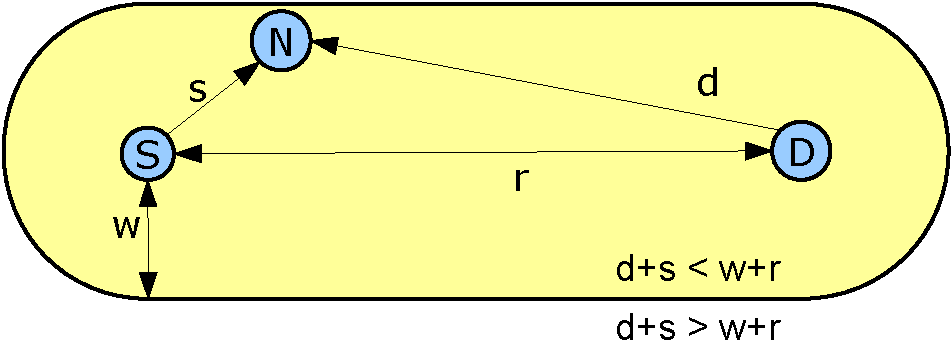
\includegraphics[width=\textwidth]{img/channel}
\caption[Distributed channel]{Construction of a distributed channel, based on distance between the two ends $S$ and $D$ ($r$), width ($w$), distance from $S$ ($s$) and distance from $D$ ($d$).}\label{f:preview}
\end{figure}


\section{From gradient to distributed channel}
\begin{figure}
{\footnotesize \begin{Verbatim}[samepage=true, frame=single, commandchars=\\\{\}]
% ChannelSource: initiates the channel propagation
?BND_GRAD := new(eco:bond_prop = app:type, eco:bond_value = app:grad);
?SRC := new();  % the source LSA initing channel propagation
iterate \{   
  ?BND_GRAD.obs(app:distance = ?R);         % perceiving POI's gradient
  ?SRC.upd(app:src = true, app:type = app:rng, 
           app:range = ?R, app:width = ?W)            % updating source
  :
  ?SRC.upd(clear);
\}

%ChannelService: computes the final channel data structure in each node 
?BND_DST := new(eco:bond_prop = app:type , eco:bond_val = app:grad);
?BND_RNG := new(eco:bond_prop = app:type , eco:bond_val = app:rng);
?CHN := new(app:type = app:chn, app:active = "false");
iterate \{  % observes ?D,?S,?R,?W and computes channel activation flag
    ?BND_DST.obs(app:distance = ?D);
    ?BND_RNG.obs(app:distance = ?S, app:range = ?R, app:width = ?W);
    ?CHN.upd(app:active = eval("?S + ?D < ?R + ?W"));
    :
    ?CHN.upd(app:active = "false");
\}

% SteeringService
?BND_LOC := new(eco:bond_prop = eco:location, eco:bond_value = "true")
?BND_CHN := new(eco:bond_prop = app:type app:active)
?BND_FIE := new(eco:bond_prop = app:temp, eco:bond_value = "false");
?DIR := new();
iterate \{
  ?BND_CHN.obs(app:active = "true"); ?BND_LOC.obs(eco:location = ?MYLOC); 
  ?BND_FIE.obs(app:location = ?DIRLOC); 
  ?DIR.upd(app:direction = eval("?MYLOC - ?DIRLOC"))
  :
  ?DIR.upd(empty); 
\}

\end{Verbatim}
}
\caption{Multi-agent system for the distributed channel}
\label{f:mas}
\end{figure}
%
On top of a gradient structure one can set up a steering service that activates all the signs located along an optimal path from an area $S$, where interested people are initially located, to the POI $D$. 
%
Such a path should also have a given ``width'' to take into account the variability of people movement.
%
The resulting spatial structure can be referred to as a (distributed) \emph{channel}, and should be created by self-organisation in a way that it can, again, automatically adapt to the presence of obstacles and to changes in the environment---see a preview in \Cref{f:preview}.

\begin{figure}
\begin{center}{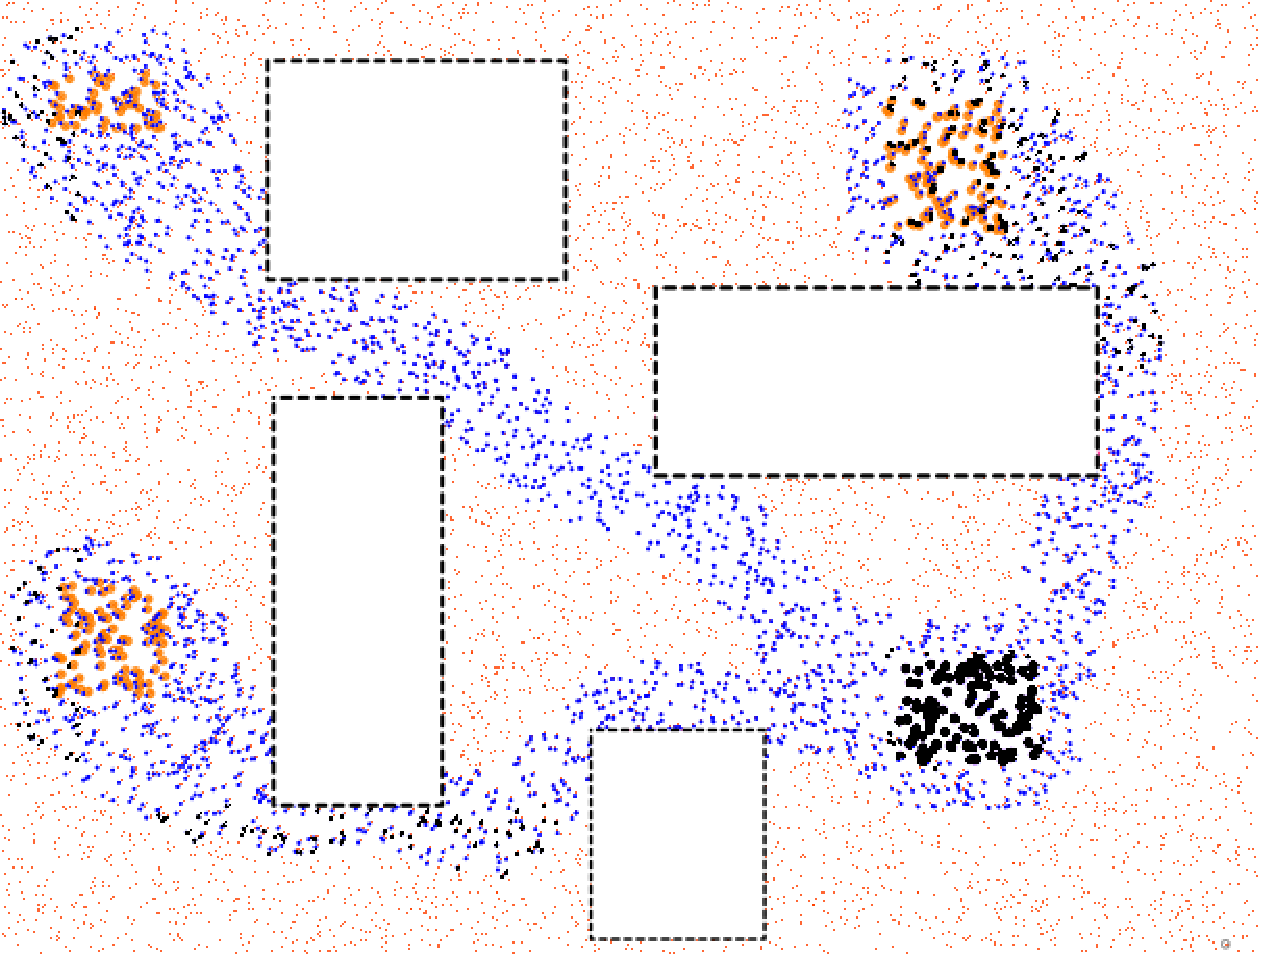
\includegraphics[width=\textwidth]{img/continuous_black}}\end{center}
\caption[Channels routes in a dense distributed environment]{Channels (blue) route between source (orange) and destination (black), deployed in a high-density environment of 10'000 nodes (right) with blank areas acting as obstacles.}
\label{f:channel}
\end{figure}

A solution to this problem can be conceived following the general approach of ``spatial computing'' \cite{SpatialIGI2013,V-SCW2013,proto}, namely, functionally composing simpler gradient-based data structures.
%
It can be coded in our process algebraic language as shown in \Cref{f:mas}, with the behaviour of the following $3$ kinds of agent.

First a \emph{channel source} agent located at position $S$ is in charge of bonding with the gradient spread from position $D$, and accordingly creates a source LSA \texttt{?SRC} which will be continuously updated to reflect the current distance \texttt{?R} from $S$ and $D$, and to carry also the width value \texttt{?W}.
%
The gradient agent defined in \Cref{f:grad} will be able to create a new gradient out of this source LSA, which will propagate carrying both \texttt{?R} and \texttt{?W}, in addition to the distance from $D$ associated with the  \texttt{app:distance} property.

Then, a \emph{channel service} agent is able to finally create the channel LSA: it bonds and observes both gradients, and the sets a flag into a newly created (and continuously updated) LSA depending on whether the node is inside or outside the channel area, as described in \Cref{f:preview}.

Finally, a \emph{steering service} agent has the goal of reifying a sign towards the direction of area $D$ only in nodes inside the channel area: this is achieved by retrieving the current location (\texttt{eco:location}) and the location  of the neighbouring node with smallest distance value from $D$ (held in \texttt{app:location}) and performing a subtraction operation---the semantics of this subtraction depends on the actual shape of coordinates used for identifying locations.
%
The LSA it produces and maintains is representative of the direction of the sign to be shown on pervasive displays, and is intended to be observed by a display agent.

\section{Simulation in \alchemist{}}

\begin{figure}
\begin{center}{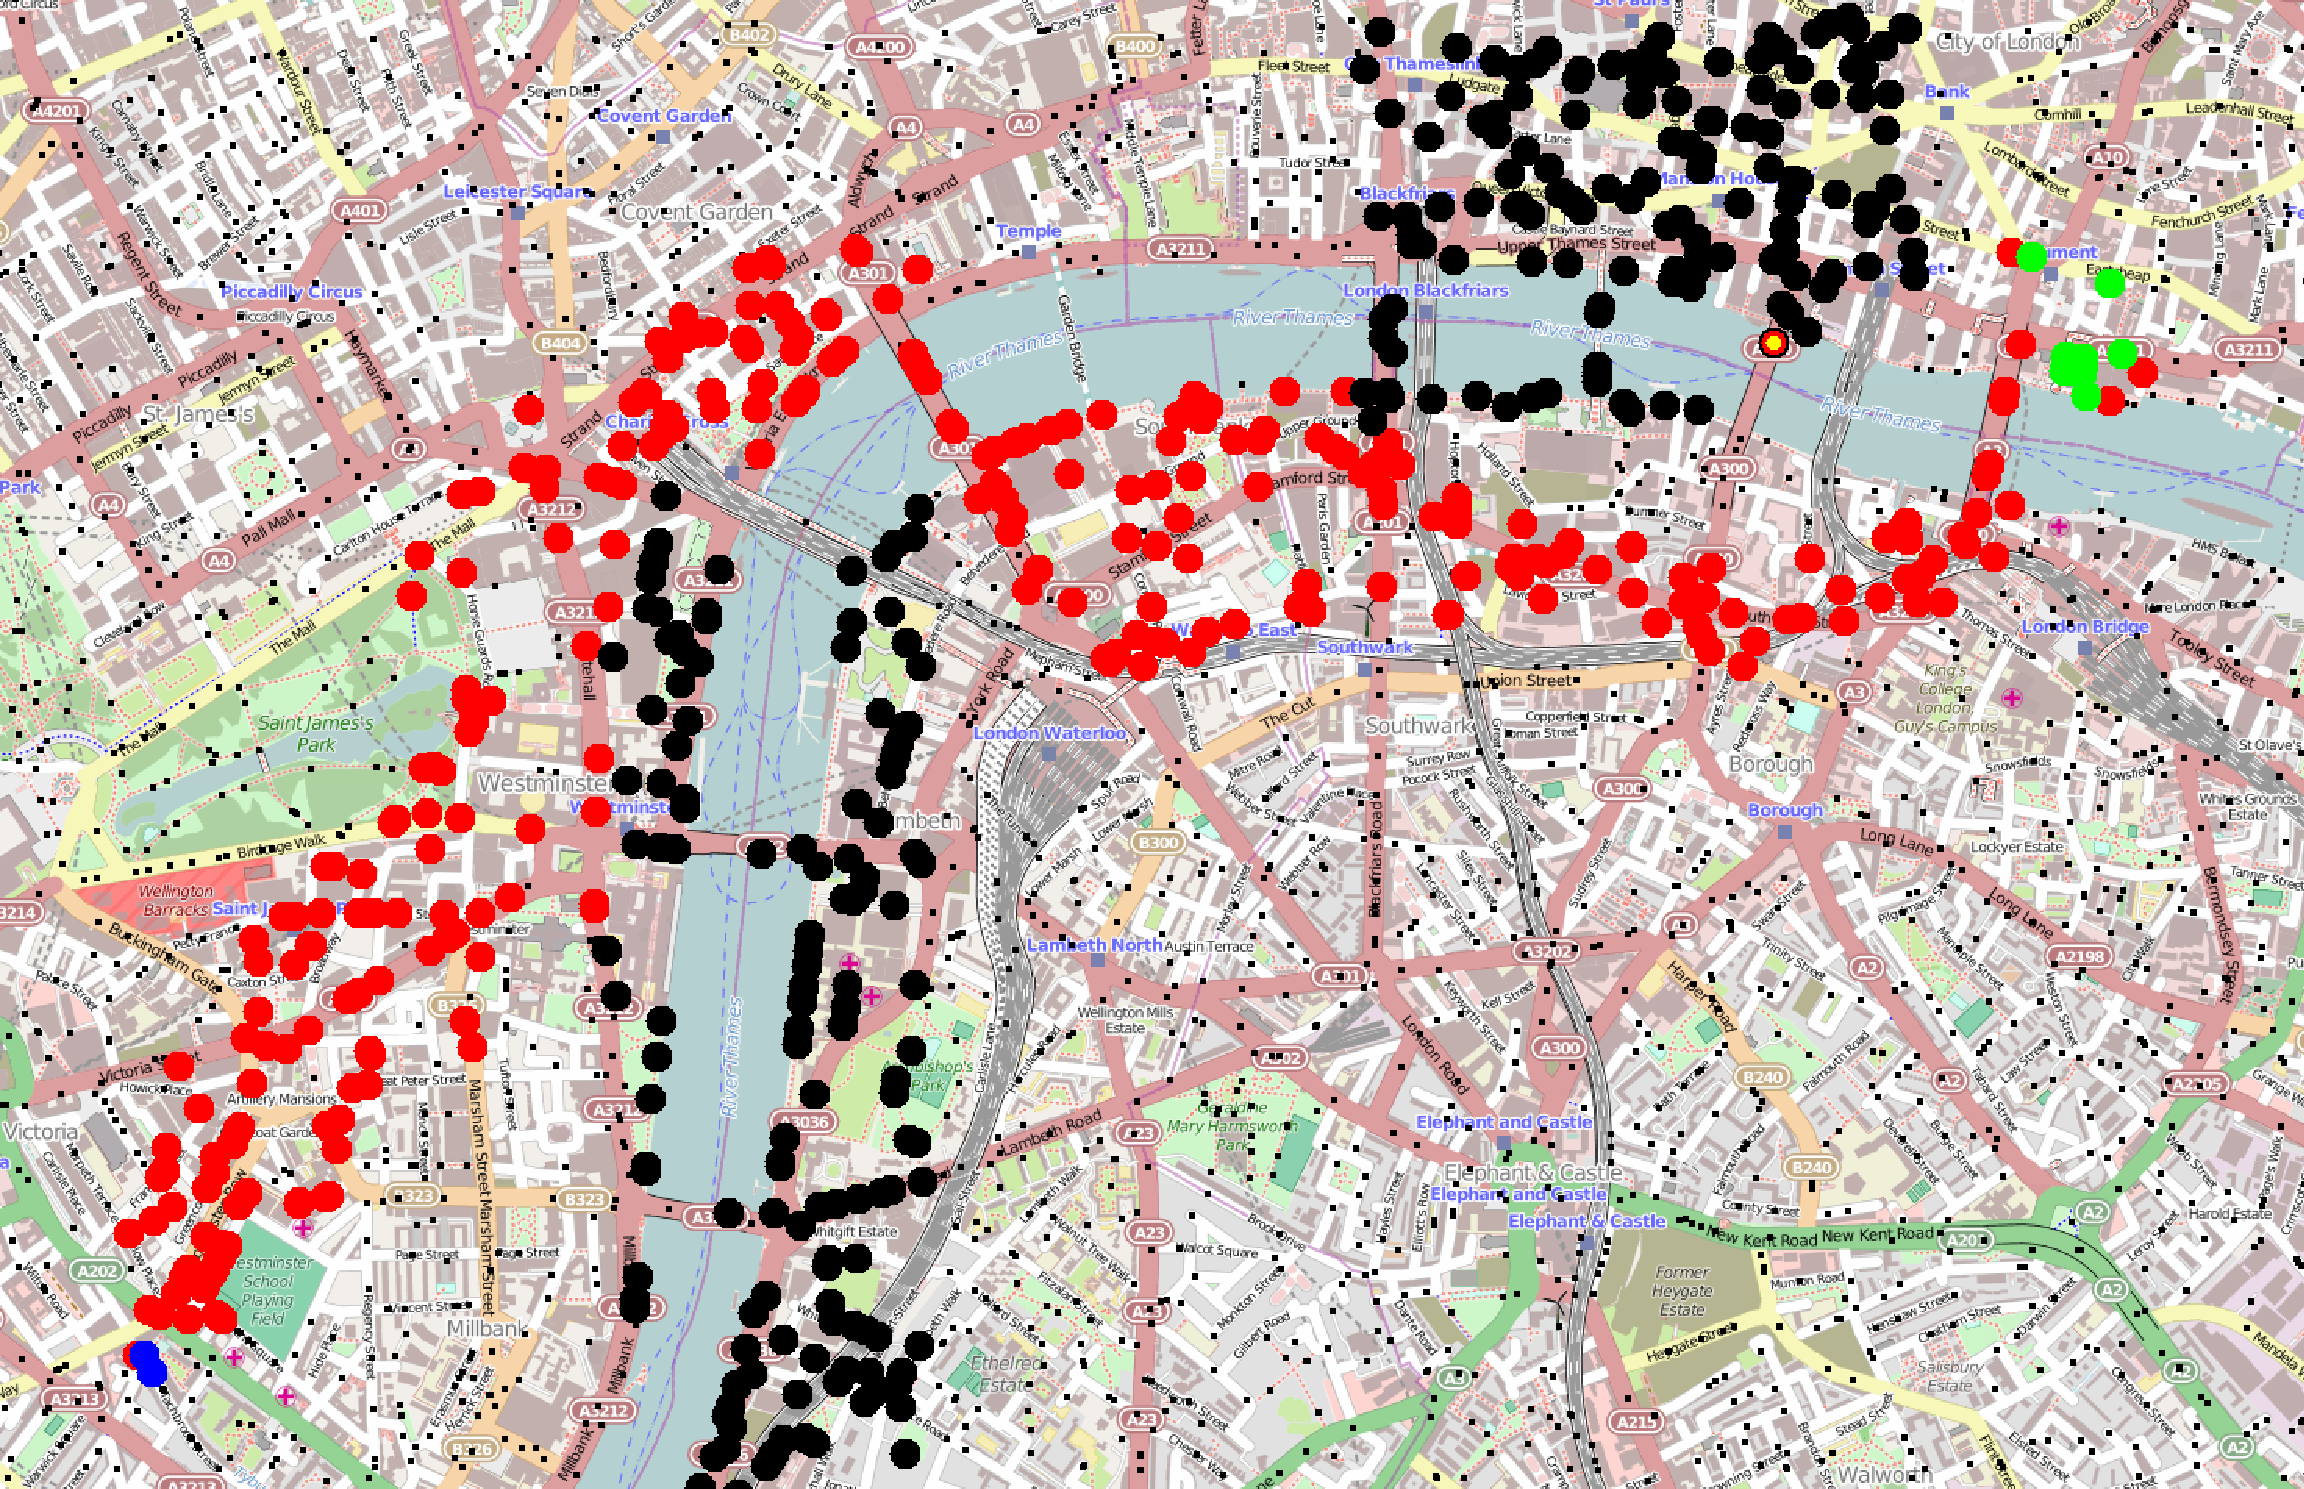
\includegraphics[width=\textwidth]{img/london-channel}}\end{center}
\caption[Channel deployed in London]{The distributed channels deployed in a smartcity (London) for pedestrian steering. Red nodes represent devices inside the channel area, while black nodes correspond to ``obstacle'' areas.}
\label{f:london}
\end{figure}

\begin{figure}
\begin{center}{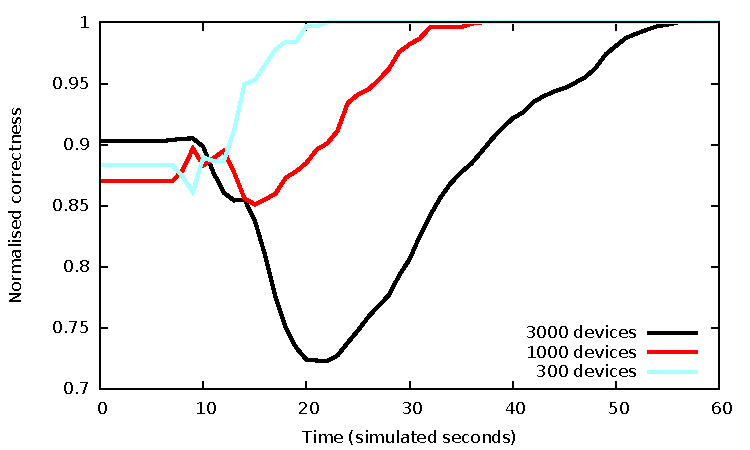
\includegraphics[width=\textwidth]{img/quality}}\end{center}
\caption[Devices correctly building the channel]{Percentage of devices correctly showing channel information over time, using topologies with different densities.}
\label{f:london2}
\end{figure}

\begin{figure}
\begin{center}{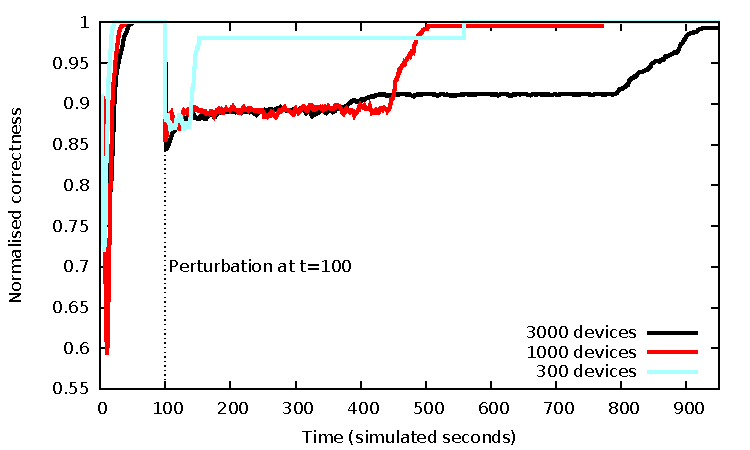
\includegraphics[width=\textwidth]{img/addobstacle}}\end{center}
\caption[Devices correctly building the channel, with a new obstacle]{Percentage of devices correctly showing channel information in the presence of addition of an obstacle.}
\label{f:london3}
\end{figure}

\begin{figure}
\begin{center}{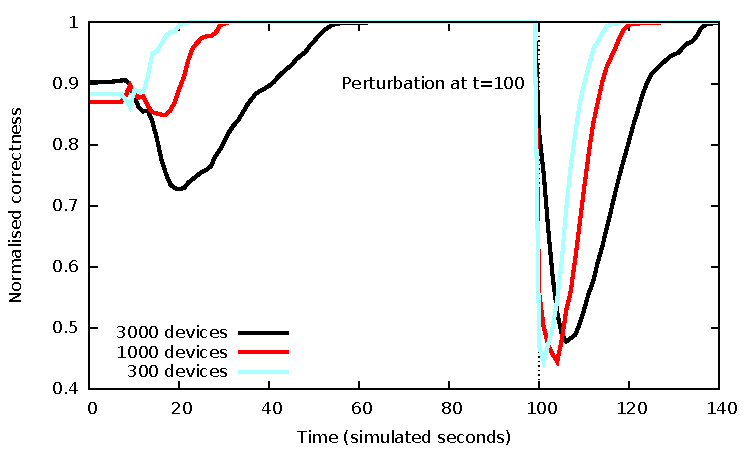
\includegraphics[width=\textwidth]{img/removeobstacle}}\end{center}
\caption[Devices correctly building the channel, removing an existing obstacle]{Percentage of devices correctly showing channel information in the presence of removal of an obstacle.}
\label{f:london4}
\end{figure}



We provide a brief qualitative and quantitative account of the behaviour of the channel distributed data structure, with the goal of validating the design of agents as defined above.

We first discuss some qualitative aspects, with help of the snapshot in \Cref{f:channel}, showing the result of a simulation of a channel structure in a high-density network, created by running an equivalent model in the Proto simulator \cite{proto}.
%
First, one can note that the resulting channel data structure is highly independent of local aspects of network topology: provided that nodes are spread more or less randomly, only density affects the final shape, and in particular, the ``width'' of the channel\footnote{This is because we used a hop-count-gradient to propagate distances: full independence of density can be achieved by suitably reifying estimated distances between nodes as proper LSAs, and using such information when re-aggregating LSAs---which we did not develop for the sake of simplicity.}.
%
Second, the way the channel is created allows one to use distributed concepts of ``source'' and ``destination'' of a channel, and even to consider the case of a channel starting from multiple sources---e.g., to guide different groups of interested people.
%
This is because self-organisation is achieved here by the functional combination of well-engineered spatial structures, as advocated in works such as \cite{SpatialIGI2013}.
%
Third, this structure automatically adapts to the shape of the network, properly bypassing obstacle areas.
%
This happens since it can be shown that the diffusion-aggregation process underlying gradients enjoys self-stabilisation as defined in \cite{VD-COORD2014-LNCS2014} (diffusion always increments distance, and aggregation is performed based on minimum values).

The presented technique can hence be usefully employed in complex environments, where it is difficult to predict the contingent situations.
%
We consider, as an example scenario, pedestrian steering in smartcities.
%
\Cref{f:london} shows a snapshot of a simulation corresponding to a deployment over a London map.
%
Devices were displaced with different density for each experiment, totalling 300, 1000 and 3000 devices respectively.
%
Devices are located on streets available to pedestrians, and device connections are based on proximity.
%
We considered as the POI Monument Street, and created a channel starting from the Royal Horticultural Society, where interested people may be initially located.
%
Dark nodes are those in which some form of unfavourable condition is assumed to be detected, requiring dynamic re-route along different paths.

From a qualitative point of view, \Cref{f:london} confirms the self-adaptive character of the distributed channel data structure, as we discussed above.
%
From a quantitative point of view, we measured the time for this data structure to establish under different conditions.
%
Starting from the basic scenario depicted in \Cref{f:london}, in \Cref{f:london2} we investigated the time needed to reach a full stabilisation of the correct channel data structure. It charts the percentage of nodes which reached the correct final state over time.
%
The result is that stabilisation is always eventually reached, in an average time that grows linearly with network diameter.
%
The speed of information diffusion is approximatively computed as the distance of nodes multiplied by the frequency at which they run the computation round of eco-laws.
%
\Cref{f:london3} and \Cref{f:london4} study self-stabilisation in response to changes in the environment, corresponding to the addition/removal of all obstacles shown in \Cref{f:london}, which requires a complete (spontaneous) re-calculation of the path.
%
These charts confirm the estimation of stabilisation time studied in \cite{crf}.
%
Namely, the repair time is much faster with removal of obstacles, since in this case gradient values quickly fall down to their new values (i.e., distances quickly decrease).
%
On the other hand, with obstacles added instead, values more slowly grow to the new stable state.
%
This happens because of the issue of slow ``raising values'' pointed out in \cite{crf}.


\chapter{Pattern: Anticipative adaptation}
\label{anticipative-gradient}
We note that -- to the best of our knowledge -- existing techniques studied for Gradients (see e.g. \cite{flexiblegradients,VCMZ-TAAS2011,sapereecolaws-sac2012}) tackle only present-awareness, that is, they adapt to events only at the time they occur.
%
In this\levelText{}, we are instead concerned with how Gradients can be equipped with \emph{anticipative adaptation}, namely, how they can take advantage of the local availability of information about future events, once this has been provided by some component in charge of situation recognition \cite{YeDM12}.
%
Our idea is to use such a knowledge in advance to stretch and deviate certain parts of a Gradient structure so as to promote alternative paths that could be longer, but guarantee to eventually circumvent any forbidden area so as to reach the target in shortest time.
%
Following the self-organisation approach, this will be realised in an emergent way, relying only on local interactions and without any supervision.
%
Example scenarios where this mechanism can be useful include traffic management, to tackle pre-scheduled road constructions, availability of historical formation about traffic jams in certain areas of a city, known timing of opening bridges or railroad crossing, and so on.
%
It can also be used in crowd steering applications based on signs appearing in public displays \cite{sapereecolaws-sac2012}: e.g., in a large exhibition centre the scheduling of popular and typically crowded exhibitions can be considered with the goal of anticipating and preventing the formation of crowds.

\section{Anticipative Gradient}

We conceive a new self-organisation mechanisms built upon the above Gradient pattern to tackle anticipative adaptation, namely, ensuring that the retrieval of the gradient source proactively reacts to available information about future events, namely, impossibility of transiting across a given area---e.g. modelling interruptions of roads in traffic control applications.
%
In this\levelText{}we first motivate and analyse the problem, then elaborate a solution based on a combination of mechanisms related to the gradient pattern, and finally check the general correctness of the result by some simulation.

\subsection{Motivations and problem analysis}

A basic application of the Gradient pattern is to steer a requester from its current location to the Gradient's source location---namely, what is called Chemotaxis pattern in \cite{FDMVA-NACO2012}.
%
Such a requester (which we here generally refer to as an agent) can either be a mobile software agent roaming a network to find proper information, a person guided in a complex environment by signs dynamically appearing in its smartphone \cite{mass2011}, a car which is given traffic control suggestions through its navigation system, or an information item directed to the target of a communication \cite{VCMZ-TAAS2011}.
%
It is quite standard to make the Gradient field adapt to contingencies as soon as they appear: for instance, interruption of a road can reflect into a change of the network topology, leading to the automatic recalculation of the Gradient structure to identify a new path towards the target of interest.
%
Following that line, in \cite{sapereecolaws-sac2012} it was studied how dynamically-formed crowded areas can be perceived as areas to be circumvented by other people roaming the environment.

We address the design of a different mechanism which, to the best of our knowledge, has never been considered so far: how Gradient-based self-organisation mechanisms can be extended to deal with the case in which in some node(s) there is knowledge about an event that will occur there in the future and prevent/modify the ability of an agent to transit across the node.
%
Taking advantage of such information, one could think of a strategy to spread this information around such that -- in an emergent way -- the Gradient can somewhat deviate to anticipate the effect of the future event, possibly promoting a path that could be longer but guarantee to circumvent the forbidden-area eventually reaching the target in shortest time.
%
There are several example applications for one such mechanism, tackling the availability of information about future road constructions, statistic formation of traffic jams in certain areas of a city, timing of opening bridges or railroad crossing, scheduling of popular and typically crowded exhibitions in a museum, and so on.

We aim at designing a solution that is not tight to a specific application context, but has the same level of generality of the Gradient pattern.
%
As such we assume -- in continuity with the basic hypothesis used for the Gradient pattern -- that the environment is densely covered with computational nodes hosting annotations and forming a topology reflecting the structure of the environment (and hence its ability of being roamed by agents).
%
We also assume that in each node estimated ``distance'' to all neighbours is available: such a distance should measure the expected average time needed for an agent to move from one location to another---here we will rely on general ``time units'' without any correspondence with a physical time.
%
The underlying middleware is in charge of keeping this information lively updated, such that formation of crowded areas are automatically reflected into a higher distance of the link between two nodes, thus making a path including such a link less appealing---accordingly, we will not consider crowd information further.
%
We hence refer to \emph{agent-speed} as the non-uniform ratio between physical distance and estimated transiting time at each location.

In some node of the network there could be some (future-aware) situation recognition component \cite{YeDM12} in charge of intercepting a future event, namely, what happens and when.
%
We shall focus on events concerning impossibility of transiting across the node, expected in the period of time in the future in between $Ts$ and $Te$ ($Ts<Te$) time units from current time.
%
Our basic strategy, detailed below, is to make information about such (possibly multiple and overlapping) events spread around, and suitably combine with a Gradient created to reach a target of interest.
%
The result of such a combination, what we call an Anticipative Gradient, will be used by agents to navigate towards the target of interest along optimal, dynamically computed paths taking in consideration those future events.
%
According to the self-organisation style, such mechanisms will be based only on local interactions, and will be carried on without any global supervision.

\subsection{Spatial structures}

\subsubsection{Horizon Wave}

A first component in our strategy is the advertisement of a future event (FE). We call FE area the set of nodes that will host such an event.
%
Advertisement of the FE needs not require full-space and -time propagation, but -- at a given time -- it should reach only the set of nodes that might be concerned by the FE, namely, those from which an agent moving towards the FE area would actually reach it when the FE actually occurs.
%
In a sense, the set of points in space and time that should be advertised resembles the notion of event horizon in physics, though it is here located in the past and propagates at the agent-speed.
%
This is why we refer to this pattern as Horizon Wave (or Wave for short).

We consider for simplicity a uniform and continuous 2D environment, allowing us to better grasp the behaviour of the proposed mechanisms.
%
There, a Wave defines a (circular) crown-like region of space that, as time passes, shrinks into the FE area at the agent-speed, until completely disappearing as shown in \Cref{fig:wave}.
%
Agents outside this spatio-temporal data structure needs not be concerned about the FE.

\begin{figure}
	\begin{center}
		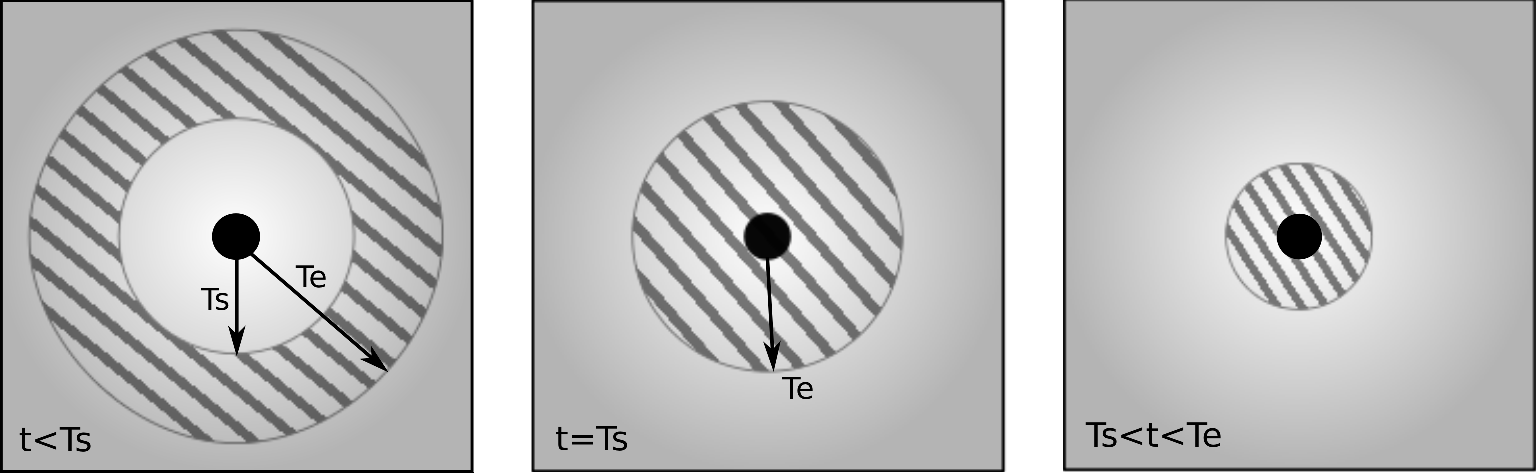
\includegraphics[width=\textwidth]{img/wave}
\end{center}
\caption[Horizon Wave pattern]{Horizon Wave pattern, with its shrinking dynamics in evidence.}
\label{fig:wave} 
\end{figure}

This spatial structure can be obtained on top of the Gradient pattern as follows.
%
We let the FE area be source of a Gradient, and any of its annotations (as diffused by the spreading process) carry information about $Ts$ and $Te$.
%
A node of the network is then inside the Wave if $Ts\leq D \leq Te$, where $D$ is the node's distance from the FE area as reified by the Gradient annotation available locally.


\subsubsection{Gradient Shadow}
\begin{figure}
	\begin{center}
		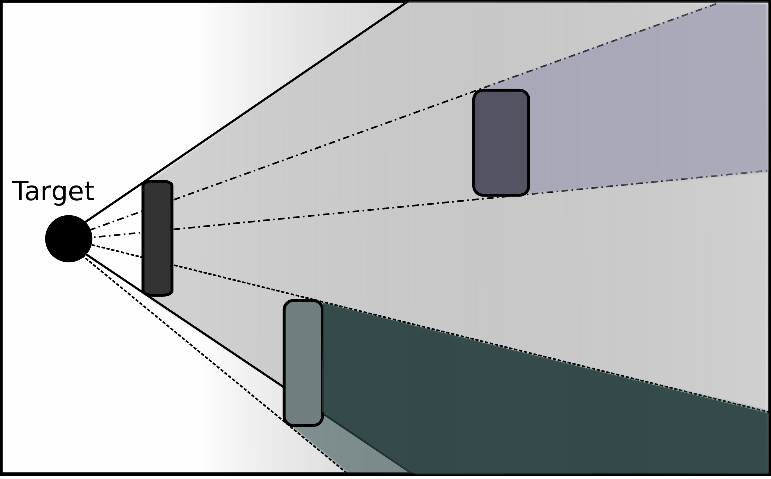
\includegraphics[width=\textwidth]{img/shadow}
\end{center}
\caption{Shadow spatial structure with overlapping Future Events}
\label{fig:shadow} 
\end{figure}

In order to understand whether an agent should actually care about circumventing the location of an FE, it is also important to consider its direction and target.
%
Let's focus on the Gradient generated by a target $p$ that an agent is directed to.
%
We should properly tag the portion of such a Gradient from which an agent, while steered towards $p$, would eventually transit across an FE area.
%
Such a portion is here called Gradient Shadow (or simply Shadow), for it recalls the shadow that the FE area would cause if it were an opaque object and the gradient source would be a source of light.
%
\Cref{fig:shadow} emphasises that the Gradient we create out of a target of interest should be able to possibly tag different, overlapping Shadows, reflecting the existence of many FEs around.

\begin{figure}
	\begin{center}
		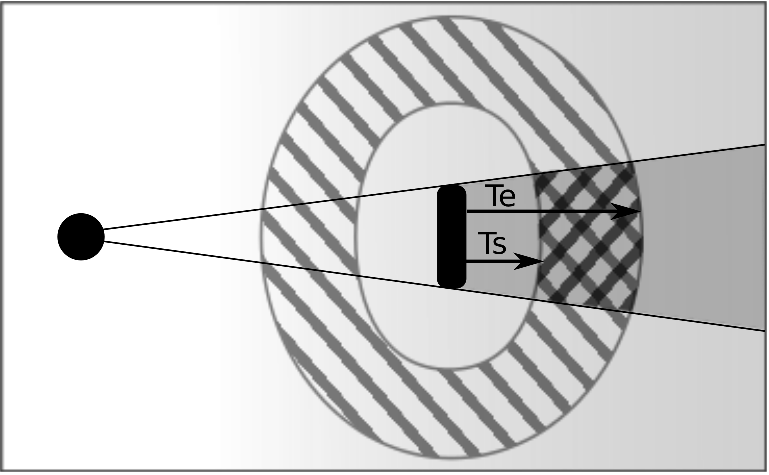
\includegraphics[width=0.9\textwidth]{img/warning-rettangolare}
\end{center}
\caption{Warning spatial structure as intersection of Wave and Shadow}
\label{fig:warning} 
\end{figure}

The main strategy to create this spatial structure amounts to let Gradient propagation track, with a proper tag in the annotation, when it crosses an FE area: by successive propagation the tag will be reified across the whole Shadow.
%
Most specifically, this is achieved by a new chemical-like rule, matching two annotations located in the same node: the gradient annotation spread from a target $p$ and the annotation of a FE $e$.
%
The effect of the rule is to update the former annotation, adding $e$ to the list of ``tags'' it should carry.
%
Additionally, we update the aggregation law such that only Gradient annotations having the same list of tags will be aggregated.
%
In the case of a single FE $e$, hence, in each node we will possibly have both the annotation tagged by $e$ and the one with empty list of tags, which respectively carry information about a route that crosses an FE and one that circumvents it.
%
In the case of multiple FEs, all combinations will be automatically generated.

Hence, the Shadow structure created from target $p$ due to FE $e$ is defined as the set of nodes whose distance to $p$ along a path crossing $e$'s area is smaller than the one circumventing it, namely, nodes having an annotation tagged with $e$ carrying a smaller distance value that any annotation that is not tagged by $e$.

Again, while targeting a given point of interest, only agents located in a FE's Shadow should be concerned about the FE, since outside that area an agent would by construction be steered to the target without crossing the FE area.
%
Note that differently from the Horizon Wave pattern, a Gradient Shadow is mostly a static structure, immutable over time: of course, it can still be subject to automatic changes due to mobility of the topology, relocation of gradient source, or interception of new future events.

\subsubsection{Future Event Warning}

Now that these two basic bricks have been defined, it is easy to identify their intersection as the portion of space -- which we call Future Event Warning (or simply Warning) -- in which the Gradient has to be deviated to anticipate the FE.
%
More generally, given a target of interest $p$, and a set $e_1,..,e_n$ of FEs, let the Global Wave be the union of the Waves of all $e_i$, then the Warning area is simply obtained by the intersection between $p$'s Shadows as created by $e_1,..,e_n$ and the Global Wave.
%
In our computational framework this area is formed by the nodes featuring the gradient annotation of a target $p$ tagged by an FE $e$ (Shadow), as well as the gradient annotation of FE $e$ whose distance is in between $Ts$ and $Te$ (Wave).

An example of such a structure for a single event is shown in \Cref{fig:warning}.
%
Considering only one event $e$, this area has the shape of a crown sector, it is located on the opposite side of $e$ with respect to the gradient source, and it moves towards $e$ until vanishing.


\subsubsection{Anticipative Gradient}

\begin{figure}
	\begin{center}
		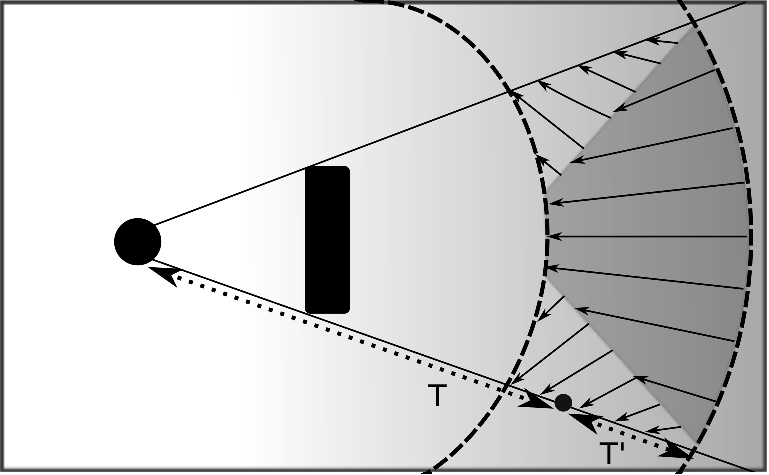
\includegraphics[width=\textwidth]{img/anticipatory_field}
\end{center}
\caption{Anticipative Gradient pattern (and ``waiting distance'' $T'$).}
\label{fig:aa} 
\end{figure}

\begin{figure}
	\begin{center}
		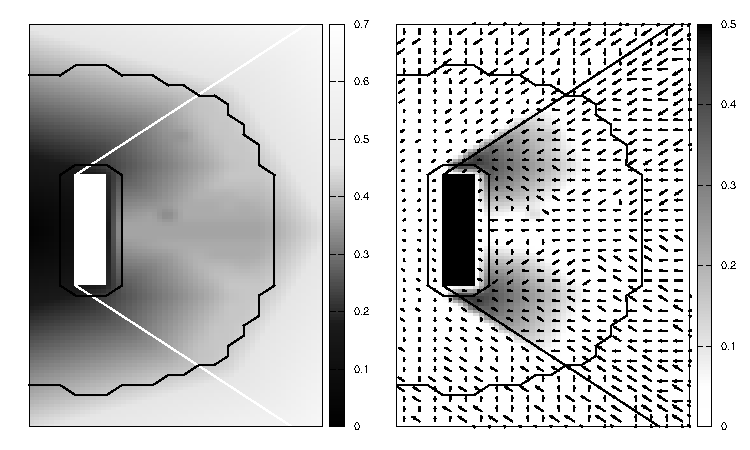
\includegraphics[width=0.9\textwidth]{img/matrix}
\end{center}
\caption[Anticipative Gradient]{An Anticipative Gradient case: (Left) estimated distance normalised by the maximum value; (Right) time-to-destination improvement factor and steering direction.}
\label{fig:2d} 
\end{figure}


We now define the most important self-organisation pattern emerging from the combination of the above ones, namely, what we call the Anticipative Gradient.
%
Starting again from a target $p$, and a set of future events $e_1,..,e_n$, this is identical to a standard Gradient outside the Warning area, since there agents can be steered to $p$ without any special management.
%
Inside the Warning area of an FE $e_i$ instead, distance and orientation values in each node should reflect the optimal path among the two following alternative: the one crossing $e_i$ and the one circumventing it.

An additional caveat is how we can compute the actual time-to-destination (i.e., distance) of a node $n$ in the Warning area along a path crossing an FE $e$---since using that path will make the agent experience the obstacle in the future.
%
A possibility for an agent would be to wait in $n$ until it is outside the Warning area and then move towards $e$ and then to $p$. 
%
Alternatively, it could immediately move from $n$ towards $e$, and be stuck there until the Wave is over---it can be shown that the strategy of circumventing the FE area instead of staying stuck is never winning over the one finding a path circumventing $e$ since the beginning.
%
In any strategy, the time-to-destination is the one obtained without considering $e$ ($T$), plus a \emph{waiting distance} ($T'$) measuring the distance of $n$ to the outside margin of the Wave (namely, the waiting time the agent would be forced to)---see \Cref{fig:aa}.
%
Note that in the case $n$ is simultaneously inside many different Warning areas, the distance value should be increased by the waiting distance computed for each of them.

\begin{figure}
	\begin{center}
		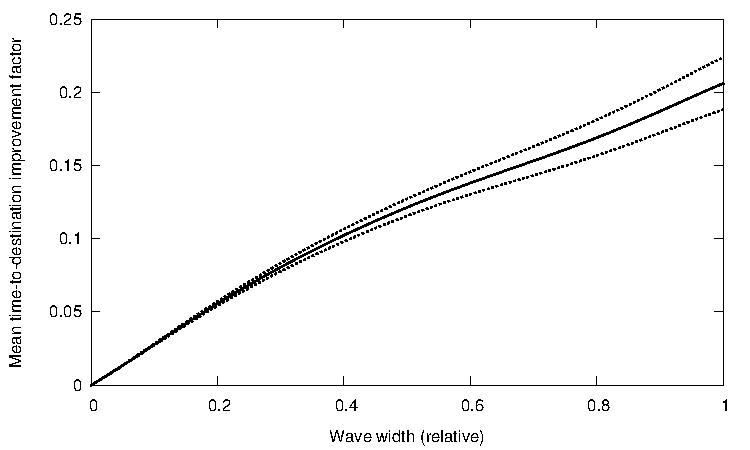
\includegraphics[width=0.9\textwidth]{img/processed}
\end{center}
\caption[Anticipative Gradient performance]{Mean time-to-destination factor (and standard deviation) in the Warning area, measured with different widths of Horizon Wave (normalised to grid size).}
\label{fig:sims}
\end{figure}

\Cref{fig:aa} also qualitatively depicts what are expected directions in a Warning area.
%
On the one hand, near the end of the Wave and in central position there is relatively little advantage in trying to circumvent the future event location, for the strategy of moving towards the FE anyway is winning. Hence, the orientation is towards the FE. In that region, we expect a rather uniform time-to-destination.
%
On the other hand, at the beginning of the wave and in lateral positions of the Warning area the steering service will likely redirect an agent laterally outside the Warning zone to bypass the FE area.

More precisely, the Anticipative Gradient can be created out of two additional laws working as follows.
%
The first law simply takes the Gradient annotation generated from a target, and clones it into a unique new annotation for the Anticipative Gradient: at this stage the two annotations will report the same distance $D$ from the source.
%
The second law matches the annotation $a$ of an Anticipative Gradient as created above with the annotation $w$ of the Wave of an FE $e$: its result is that $e$ is removed from the list of tags in $a$, and $a$'s distance is increased by $e$'s waiting distance as discussed above, computed as $T_e-D$. 
%
Note such a law would iteratively fire to match $a$ with the waves of all active (overlapping) FEs, until $a$'s list of tags is emptied.

The neat result is that the Antipative Gradient is identical to the standard Gradient outside Warning areas, it instead selectively reports augmented distances in Warning areas, such that following the route towards nodes with minimum distance to the target always guarantee to efficiently avoid obstacles appearing in the future.


\subsection{Simulations}

We checked the basic correctness of the proposed self-organisation pattern by simulation, conducted using \alchemist{}.

\Cref{fig:2d} (left) shows a pictorial representation of how the Anticipative Gradient looks like in a simulation of a 2D grid of 60x30 nodes, with a white-coloured rectangular-like FE. \Cref{fig:2d} (right) shows what would be the right direction proposed at that time in each node. The analysis of these data confirms the expected qualitative results, in analogy with \Cref{fig:aa}. Namely, in the Warning area there is a whole triangle-like sector in which the estimated distance is higher (lighter colour) and constant---due to the waiting-time an agent has to experience. There, the proposed direction does not circumvent the FE. Instead, in the upper and lower border of the Warning area the Anticipative Gradient would tend to steer an agent away from the FE.
%
\Cref{fig:2d} (right) also shows what is the relative improvement an agent would experience when starting from the different locations of the network thanks to the anticipation of the future event. It ranges from a 50\% in nodes near the left border of the Warning area to a 0\% in nodes outside the Warning area.

\Cref{fig:sims} shows what is the average (with standard deviation) improvement for nodes in the Warning area depending on the width of the Wave. Clearly, there is a greater improvement in using the Anticipative Gradient pattern in those cases where the future event lasts longer, namely, with higher width ($Te-Ts$) of the Wave.

\chapter{Case Study: Crowd evacuation}

\begin{figure}
    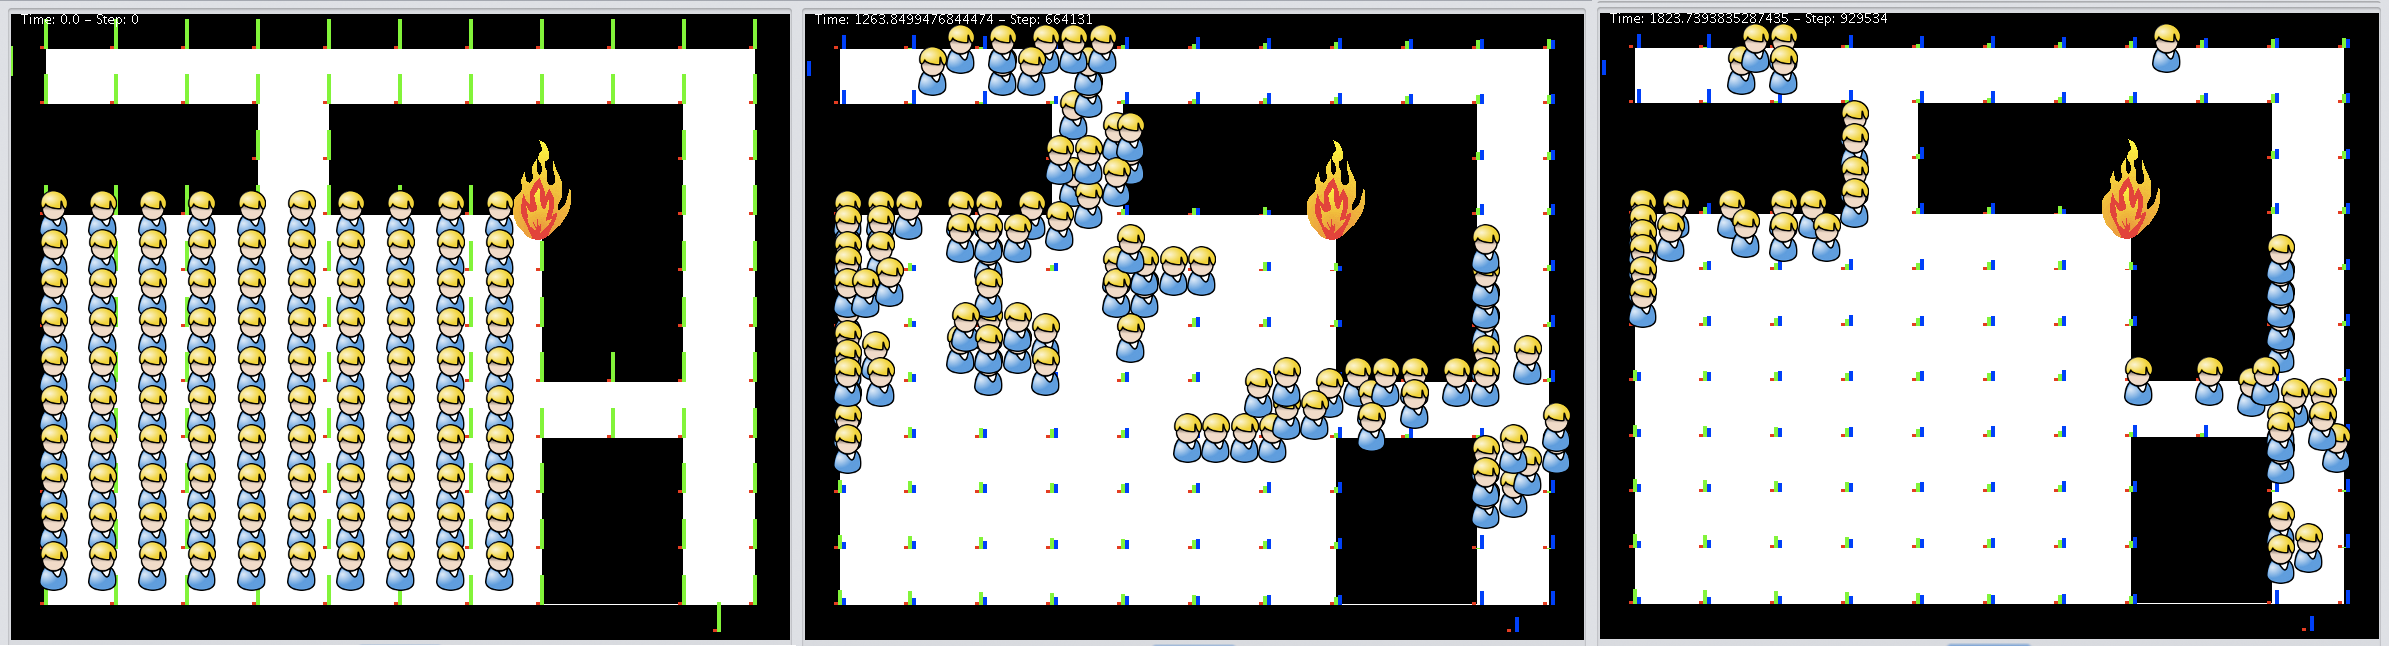
\includegraphics[width=\columnwidth]{img/run}
    \caption[Reference exposition for crowd evacuation]{A simulation run of the reference exposition: three snapshots\label{fig:generalmap}}    
\end{figure}


\section{A crowd evacuation application}

A public exposition is taking place in a museum composed of rooms, corridors, and exit doors. \Cref{fig:generalmap} shows the layout of the exposition.
%
The surface of the exposition is covered by sensors, arranged in a grid, able to sense fire, detect the presence of people, interact with other sensors in their proximity as well as with PDAs that visitors carry with them. 

When a fire breaks out, PDAs (by interaction with sensors) must show the direction towards an exit, along a safe path. The system has to be resilient to changes or unpredicted situations, in particular the safe path must consider: \emph{(i - distance)}: it should tend to lead to the nearest exit; \emph{(ii - fire)}: it should tend to stay away from fire; and \emph{(iii - crowd)}: it should tend to avoid overcrowded paths.
%
These factors  influence PDAs by means of the following LSAs:

\begin{itemize}
\item{The exit gradient:} each node contains an LSA with a numeric value indicating the distance from the nearest exit. These LSAs form a gradient field covering the whole expo.
%
Over an exit, the gradient value is 0, and it increments with distance  from the exit. When there are several exits or several paths towards an exit, the lowest distance value is kept for a node.

\item{The fire gradient}: each node also contains an LSA indicating its distance from nearest fire. The LSA's value is 0 at the fire's location and increases with distance.
%
It reaches a maximum value at a safe distance from a fire.

\item{The crowding gradient:} sensors in the expo surface detect the presence of people and adjust the value in a local LSA indicating the crowding level of the location.
%
As with exit and fire, this LSA is diffused around, and its value increases with the distance from the crowded region.

\item{The attractiveness information:} finally, each node contains an LSA indicating how desirable it is as a position in an escape route.
%
Its value is based on the values of the previous three, and is used to choose which direction displays should point to.

\end{itemize}

\subsection{Types of LSAs in the system}

There are three forms of LSAs used in this scenario:
%
{\small \[\begin{array}{l}
\lsa{\mathtt{source}, type, max, ann},\;
\lsa{\mathtt{grad}, type, value, max, ann},\;
\lsa{\mathtt{info}, type, value, tstamp}
\end{array}\]}%
%
\noindent A \textbf{source} LSA is used for gradient sources: $type$ indicates the type of gradient (\texttt{fire}, \texttt{exit}, and so on); $max$ is the gradient's maximum value; and $ann$ is the annealing factor---its purpose will be described later, along with eco-laws. 
%
A \textbf{gradient} LSA is used for individual values in a gradient: $value$ indicates the individual value; and the other parameters are like in the source LSAs.
%
Finally, an \textbf{info} LSA is used for local values (e.g., not part of a gradient)---parameters are like in the source and gradient LSAs. The $tstamp$ reflects the time of creation of the LSA.

\subsection{Building the fire, exit and crowding gradients}

The sources of the gradients are injected by sensors at appropriate locations, with the values 
$\lsa{\mathtt{source}, \mathtt{exit}, \mathtt{Me}, \mathtt{Ae}}$ and
$\lsa{\mathtt{source}, \mathtt{fire}, \mathtt{Mf}, \mathtt{Af}}$.
%
For the crowding information, we may assume that sensors are calibrated so as to locally inject an LSA indicating the level of crowding. The actual threshold in number of people will mainly depend on the sensor arrangement, and should be seen as a configuration issue. The crowding LSA will look like $\lsa{\mathtt{source}, \mathtt{crowd}, \mathtt{Mc}, \mathtt{Ac}}$ and is periodically updated by the sensor.

As sources are established, gradients are built by the following set of eco-laws, applying to exit, fire and crowding gradients by parameterising the $type$ in the LSAs.
%
First, we define eco-law \ref{law:src} that, given a source, initiates its gradient:

\begin{equation}\label{law:src}
\lsa{\mathtt{source}, T, M, A} \xmapsto{R_{init}} \lsa{\mathtt{source}, T, M, A}, \lsa{\mathtt{grad}, T, \mathtt{0}, M, A}
\end{equation}

\noindent When a node contains a gradient LSA, it spreads it to a neighbouring node with an increased value, according to eco-law \ref{law:spread}:
\begin{equation}\label{law:spread}
\lsa{\mathtt{grad}, T, V, M, A} \xmapsto{R_{s}}  \lsa{\mathtt{grad}, T, V, M, A}, \rem\lsa{\mathtt{grad}, T, \mathtt{min(}V\mathit{+}\#D, M\mathtt{)}, M, A}
\end{equation}

\noindent Due to use of the $\#D$ system variable, each node will carry a \texttt{grad} LSA indicating the topological distance from the source. When the spread values reach the maximum vale $M$, the gradient becomes a plateau. 
%
Also note that the iterative application of this eco-law causes continuous diffusion of the LSA to all neighbouring nodes. 

The spreading eco-law above  may produce duplicate values in locations (due to multiple sources, multiple paths to a source, or even diffusion of multiple LSAs over time).
%
Thus,  eco-law \ref{law:min}  retains only the minimum distance:

\begin{equation}\label{law:min}
\lsa{\mathtt{grad}, T, V, M, A}, \lsa{\mathtt{grad}, T, W, M, A} \rightarrow \lsa{\mathtt{grad}, T, \texttt{min}(V,W), M, A}
\end{equation}
%
\noindent Finally, we have to address the dynamism of the scenario where people move, fires extinguish, exits may be blocked, crowds form and dissolve.
%
If a gradient source vanishes, the diffused values should increase (e.g., the distance to exit increases if the nearest exit is no longer available).
%
However, with the above eco-laws this does not happen because eco-law \ref{law:min} always retaining the minimum value.
%
This is the purpose of the annealing parameter in the gradient LSAs: it defines the rate of  eco-law \ref{law:annealing}, which continuously tends to level up gradient values, encouraging the replacement of old values by more current ones:

\begin{equation}\label{law:annealing}
\lsa{\mathtt{grad}, T, V, M, A} \xmapsto{R_{ann}(A)} \lsa{\mathtt{grad}, T, V\mathit{+}1, M, A}
\end{equation}
%
\noindent The $R_{ann}$ rate is directly proportional to $A$. When a fire is put out, for example, this eco-law will gradually raise the fire gradient to the point where it reaches the maximum, indicating no fire.
%
Annealing may introduce a burden on the system, therefore high annealing values should only be used for gradients that have to change often or quickly.

\subsection{Ranking escape paths: the attractiveness field}

Based on exit distance, fire distance and crowding, a location can be ranked as more or less ``attractive'' to be part of an escape path.
%
This is done via an \emph{attractiveness} value automatically attached to each node by eco-law \ref{law:attr}:
%
\begin{equation}\label{law:attr}
\begin{array}{l}
\lsa{\mathtt{grad}, \mathtt{exit}, E, \mathit{Me}, \mathit{Ae}}, \lsa{\mathtt{grad}, \mathtt{fire}, F, \mathit{Mf}, \mathit{Af}}, \lsa{\mathtt{info}, \mathtt{crowd}, \mathit{CR}, \mathit{TS}} \xmapsto{R_{att}} \\
\lsa{\mathtt{grad}, \mathtt{exit}, E, \mathit{Me}, \mathit{Ae}}, \lsa{\mathtt{grad}, \mathtt{fire}, F, \mathit{Mf}, \mathit{Af}}, \lsa{\mathtt{info}, \mathtt{crowd}, \mathit{CR}, \mathit{TS}}, \\
 \lsa{\mathtt{info}, \mathtt{attr}, (\mathit{Me}-E) / (1+(\mathit{Mf}-F)+k\times(\mathit{Mc}-C)), \#T}
 \end{array}
\end{equation}

\noindent Coefficient $k$ (tuned by simulation) is used to weight the effect on crowding on attractiveness.
%
As gradients evolve, older attractiveness LSAs are replaced with newer ones ($T$ is assumed positive):
%
{\small \begin{equation}
\lsa{\mathtt{info}, \mathtt{attr}, A, \mathit{TS}}, \lsa{\mathtt{info}, \mathtt{attr}, \mathit{A2}, \mathit{TS}\mathit{+}T} \rightarrow \lsa{\mathtt{info}, \mathtt{attr}, \mathit{A2}, \mathit{TS}\mathit{+}T}
\end{equation}}

\subsection{Choosing a direction}

Each location  contains by default an LSA of the form $\lsa{\mathtt{info}, \mathtt{escape}, L, \mathit{TS}}$, where $L$ is  the direction to be suggested by the PDA.
%
In principle, the neighbour with the highest attractiveness should be chosen, but a more resilient solution is to tie the markovian rate of eco-laws to the attractiveness of neighbours, so that the highest probability is to point the best neighbour, with a possibility to point a less-than-optimal (but still attractive) neighbour:\vspace{-15pt}

\begin{equation}\label{law:escape}\begin{array}{l}
\lsa{\mathtt{info}, \mathtt{escape}, L}, \lsa{\mathtt{info}, \mathtt{attr}, A, TS}, 
    \rem\lsa{\mathtt{info}, \mathtt{attr}, A\mathit{+}\Delta, TS2} \xmapsto{R_{disp}(\Delta)} \\
 \lsa{\mathtt{info}, \mathtt{escape}, \#O},
 \lsa{\mathtt{info}, \mathtt{attr}, A, TS},  \rem\lsa{\mathtt{info}, \mathtt{attr}, A+\Delta, TS2}
 \end{array}
\end{equation}
%
\noindent 
The rate is proportional to the difference in attractiveness between the node and its neighbour ($\Delta$). The higher the $\Delta$, the higher the rate. Note that $\Delta$ is a positive value, hence  $A+\Delta$ implies that eco-law \ref{law:escape} only considers neighbours with a higher attractiveness, i.e., the PDA will not point \emph{away} from the exit.

\subsection{Resilient behaviour}
The proposed architecture is intrinsically able to dynamically adapt to unexpected events (like node failures, network isolation, exits suddenly unavailable, crowd formation, and so on) while maintaining its functionality.
%
We will now discuss a few examples of possible problems and explain how the system reacts to them.

\subsubsection{Single-node failure}

Most behaviour in this architecture is based on nodes being able to apply eco-laws and host LSAs.
%
Failure of a node clearly impacts this behaviour in some measure. A failing node (i.e., disappearing from the system) results in a physical location where no information for the displays is available, and where gradient information is not received or transmitted. 

If the failing node is a generic one (i.e, no fire or exits at that node) and its disappearance does not cause network isolation, the impact is somewhat limited.
%
Gradients will still be transmitted \emph{around} the broken node, although values will change.
%
Displays traversing a failing node will not update their direction; however, they will also never guide people towards a failing node, because it does not have an attractiveness value; they will rather steer people around the failing node.
%
This means that functionality is preserved with decreased efficiency (i.e., longer paths).

If the failing node is a node containing a fire, the consequences are more severe: the fire will not be detected.
%
PDAs will still never point the failing node on fire directly, but they will let people pass near it. One might argue that people will still see the fire; however, from the point of view of system behaviour, safety is reduced.
%
On the other hand, it can be  assumed that a serious fire would be detected by more sensors, and that  all of them failing at the same time is unlikely.

If the failing node is an exit node, functionality gets a major hit, because the whole system will lack a fundamental information for display functioning (the exit gradient).
%
If other exits are available, the system will still guide people towards them (again preserving functionality with reduced efficiency).
%
However, if the failing node ``hides'' the only available exit, the system completely fails to provide useful information.
%
This situation can be tackled by redundant source nodes near each exit.

\subsubsection{Network isolation}

When a group of failing nodes is the only connection between two parts of the network, this causes network isolation.
%
There are a few sub-scenarios to consider.
%
If the isolated section does not include exits, we find another limitation: the evacuation mechanism cannot work inside that section, as it is lacking fundamental information.
%
If the section does however contain exits, it will act as an autonomous system in itself.
%
Efficiency may be reduced but functionality will still be preserved, with an important caveat: this section of the network will ignore fires and alarms occurring in the rest of the network.
%
This may or may not be an acceptable limitation depending on the scenario.
%
For fires, it could probably be unacceptable.
%
In a general way, however, we would consider that an isolated part of the network behaving as an autonomous system is an acceptable fallback.
%
Again, redundancy is desirable for those nodes of the network that can cause isolation.

\subsubsection{Exit unavailability}

If an exit is suddenly unavailable in the expo, for instance it is broken and hence it does not open, a sensor could detect this and drop the source LSA.
%
Because of the annealing mechanism, this causes the gradient value in each node to converge to the situation corresponding to the unavailability of that door; namely, a new path toward another exit emerges and affects the behaviour of all PDAs---people would simply go back to another exit as expected.

\subsubsection{Crowd formation}

While people follow their PDAs towards the nearest exit, it is possible that a jam forms in front of certain doors or corridors: this is one of the most perilous, unexpectable situations to appear in crowd evacuation.
%
The application we set up is meant to emergently tackle these situations by means of the crowding gradient.

Assume two available corridors exist towards some exit, and from a given room people can choose to walk through any of them towards the exit.
%
If one becomes unavailable because a jam is forming the crowding gradient would emerge, reducing attractiveness along that corridor.
%
Accordingly, it is expected that people behind the crowded area start walking back and head for the other corridor, and people in the room start choosing systematically the path free from crowd, even if they do not ``see'' the problem from the room.


\section{Simulation in \alchemist{}}

The proposed system is specified by a limited set of eco-laws, equipped with CTMC semantics.
%
This specification  can be used to feed the SAPERE infrastructure and be simulated in order to check the model dynamics in advance.

\begin{figure}
  \begin{center}
  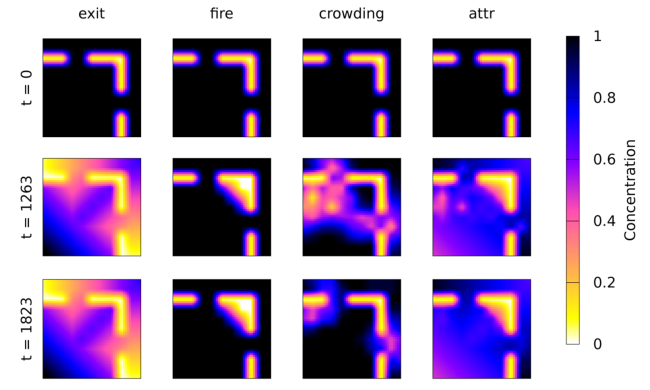
\includegraphics[width=.9\columnwidth]{img/gradient}
  \end{center}
  \caption[Gradients in crowd evacuation]{Gradients for the snaphots in \Cref{fig:generalmap}. Concentration is the gradient value normalised to its maximum value.}
  \label{fig:field}
\end{figure}

\subsection{Simulation setting}

We here present simulations conducted over an exposition structured as shown in \Cref{fig:generalmap}, where three snapshots of a simulation run are reported: all the people in the room start moving towards one of the two exists (located at the ends of the corridor) because of the fire in the top-right corner of the room.
%
Note in third snapshot that a person is walking in the middle of the corridor, for she was suggested to go to a farther exit because of the corridor jam at the bottom-right.

Rooms and corridors are covered by a grid of locations hosting sensors, one per meter in the room, one per two meters in the corridor: such locations are the infrastructure nodes where LSAs are reified.
%
The maximum values for the gradients are set to: $\mathtt{Me} = 30$,  $\mathtt{Mf}=3$,  $\mathtt{Mc}= 20$.  
%
The PDA of each person is modelled as a mobile node, able to perceive the attractiveness gradient in the nearest sensor location: accordingly, the person moves in the suggested direction.

\Cref{fig:field} shows the gradients of exit, fire, crowding and attractiveness (one per column) corresponding to the simulation steps  of \Cref{fig:generalmap} (one step per row). At $t=0$, gradients are level; with time, the gradient self-modify---it is easy to see the exits, fire and crowds in the respective gradients. 
%
The crowding gradient in the third column  changes dynamically during simulation according to the movement of people.
%
The last column shows the attractiveness gradient, computed from the other three gradients. Note how the second snapshot shows an attractiveness ``hole'' in the middle of the room  and in the corridor due to crowding.

\subsection{Tuning parameters}

\begin{figure}
  \begin{center}
  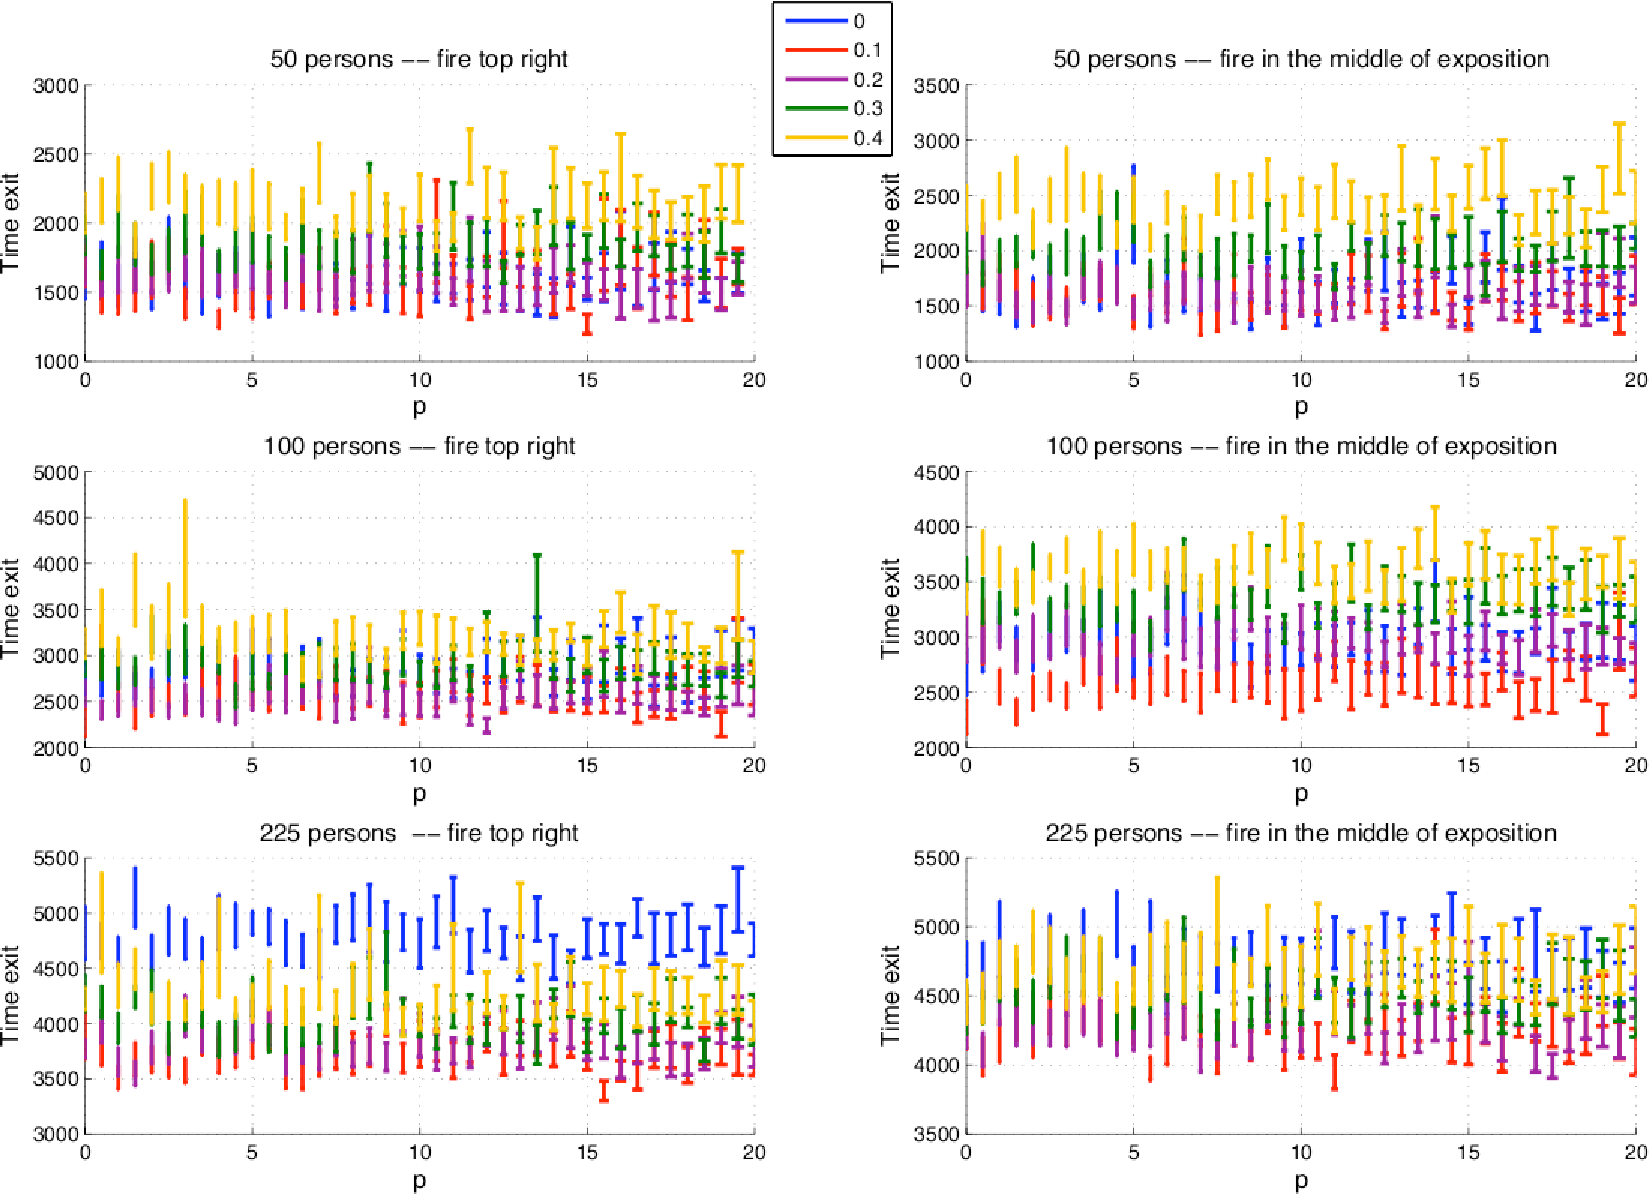
\includegraphics[width=\columnwidth]{img/allcropped}
  \end{center}
  \caption{Results of parameter analysis}
  \label{fig:results}
\end{figure}

We chose to tune by simulation two parameters of the model: $k$ (used in the eco-law computing attractiveness), and a multiplication factor $p$ we applied to the crowding gradient to control its slope---namely, how far crowding should be perceived.
%
Different simulations have been performed in order to find the set of parameters that minimises the time of exit of all the people in the room: the range of variation of $k$ is [0.1, 1] with a step of 0.1, while the range for $p$ is [0, 20] with step of 0.5. 
%
The smaller is $k$, the lower is the impact of the crowding in the computation of attractiveness, so that we expect the crowds not be avoided and the exit time to grow.
%
The bigger is $p$, the higher is the crowding gradient slope, until it becomes a local information that PDAs can perceive only very close to it. 
%
Experiments have been done with 50, 100 and 225 persons in the room and with a fire in the corner of the room or in the middle, so as to experimentally observe the impact of parameters in the evacuation outcome of different scenarios.
%
For each couple of parameters, 10 simulations have been run, considering average value and standard deviation of the resulting time.

In \Cref{fig:results} we show the results we obtained from the analysis of the parameters. 
%
Only dynamics for $k<0.5$ are shown, because the time of exit is much higher elsewhere, and also because standard deviation becomes much higher since the system is much more chaotic.

The graphs show that with $k=0$ (i.e., if the crowding gradient does \emph{not} influence attractiveness) the performance of the system slows down as the number of persons increases, and the likelihood of forming of crowds grows. This result highlights the impact of considering crowds in resilience with respect to jams.
%
For $k = 0.1$ we obtained the best performance for the system for both  simulated fire positions. Results finally showed that the parameter $p$ does not seem to have relevant impact on the average exit time in this particular expo.

\subsection{Resilience to node failures}

\begin{figure}
  \begin{center}
  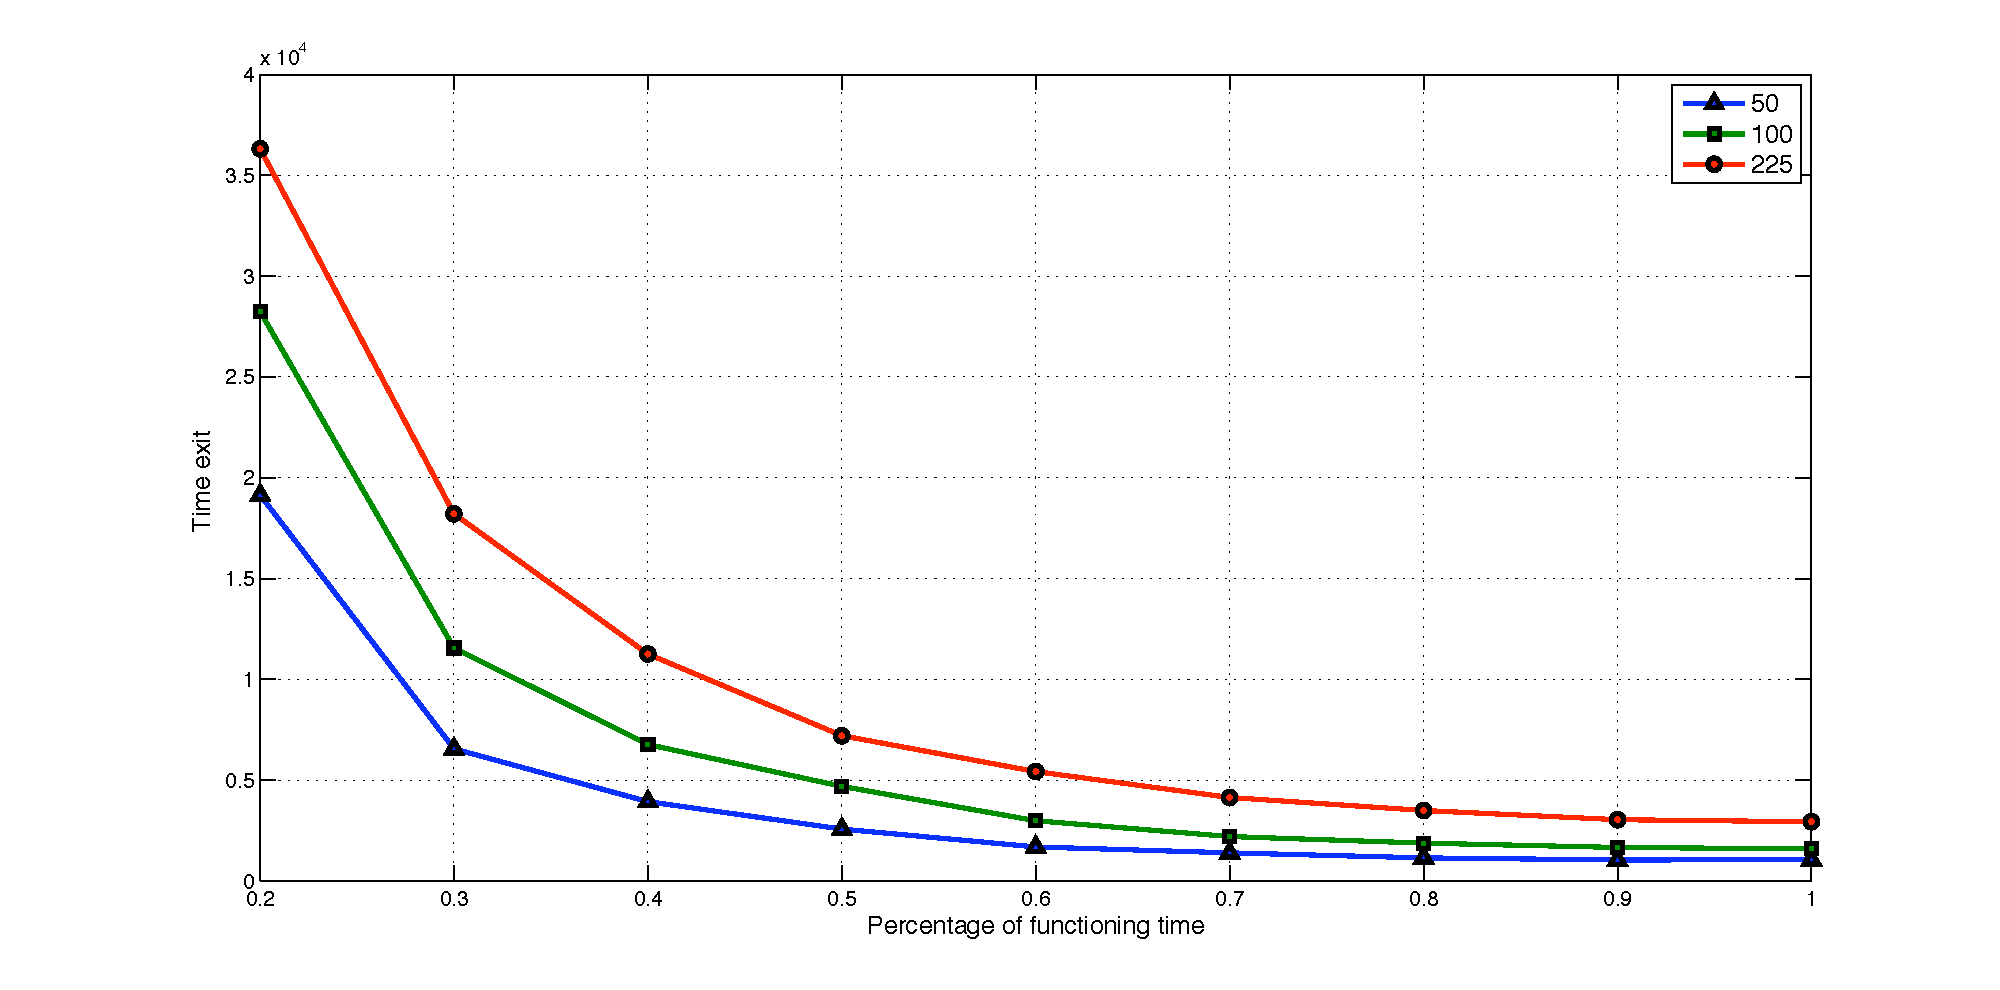
\includegraphics[width=\columnwidth]{img/resilience}
  \end{center}
  \caption{Resilience to temporary node failures}
  \label{fig:resilience}
\end{figure}

Among the many simulations analysing resilience aspects, we focused on the case in which all nodes experience temporary failures, i.e., they  work correctly only for a percentage of time.
%
We expect the system to still be safe, i.e., be able to drive people out of the room in reasonable time, in spite of the changes in gradient values around the broken nodes. 
%
The results of simulation with 50, 100 and 225 persons are shown in \Cref{fig:resilience}: the time to exit does not significantly increase even in the case of nodes failing 30\%-40\% of the time, and people are still able to eventually reach the exit even with 80\% of node downtime.


\chapter{Case Study: Crowd steering}
\label{jos-museum}
In this\levelText{}we show a crowd steering case study in which a middleware has the goal of leading people in the desired location within a complex environment in short time, avoiding obstacles such as crowded regions and without global supervisioning. 

\section{Reference scenario}

Consider a museum with a  set of rooms, whose floor is covered with a network of computational devices (infrastructure nodes).
%
These devices can exchange information with each other based on proximity, sense the presence of visitors, and hold information about expositions currently active in the museum.
%
Each room has four exits and they are connected via external corridors. Visitors wandering the museum are equipped with a hand-held device that holds the visitor's preferences.
%
By interaction with infrastructure nodes, a visitor can be guided towards rooms with a target matching their interest, thanks to signs dynamically appearing on his smartphone or on public displays.
%
This is done using techniques suggested in the field of spatial computing \cite{VCMZ-TAAS2011}---namely, computational gradients injected in a source and diffusing around such that each node holds the minimum distance value from the source.

The environment is a continuous bidimensional space with walls. 
%
Smartphones (or public displays) are agents dynamically linked with the nearest infrastructure node -- the neighbours are the sensors inside a certain radius $r$, parameter of the model -- from which they can retrieve data in order to suggest visitors where to go. Visitors are agents which follow the advices of their hand-held device (or public displays). It is defined a minimum possible distance between them, so as to model the physical limit and the fact that two visitors can't be in the same place at the same time. Visitors can move of fixed size steps inside the environment. If an obstacle is on their path, their movement is shortened to the allowed position nearest to the desired place.

\section{Steering strategy}

All the information exchanged is in form of annotations, simply modelled as tuples $\lsa{v_1,\ldots,v_n}$ (ordered sequence) of typed values, which could be for example numbers, strings, structured types, or function names.
%
\noindent There are three forms of annotations used in this scenario:

{\[\begin{array}{l}
 \lsa{\mathtt{source}, id, type, N_{max}} \\
 \lsa{\mathtt{field}, id, type, value, tstamp} \\
\lsa{\mathtt{info}, id, crowd, M, t'} \\
\end{array}\]}

\noindent A \textbf{source} annotation is used as a source with the goal of generating a field: $id$ labels the source so as to distinguish sources of the same type; $type$ indicates the type of fields in order to distinguish different expositions; $N_{max}$ is the field's maximum value. 
%
A \textbf{field} annotation is used for individual values in a gradient: $value$ indicates the individual value; the $tstamp$ reflects the time of creation of the annotation; the other parameters are like in the source annotation.
%
An \textbf{info} annotation is supposed to be created and kept up to date by each sensor. $M$ represents the number of smartphones the sensor is perceiving as neighbours.

The rules are expressed in form of chemical-resembling laws, working over patterns of annotations.
%
One such pattern $P$ is basically an annotation which may have some variable in place of one or more arguments of a tuple, and an annotation $L$ is matched to the pattern $P$ if there exists a substitution of variables which applied to $P$ gives $L$.
%
A law is hence of the kind \mbox{$P_1,\ldots,P_n\xmapsto{r}P'_1,\ldots,P'_m$}, where: \emph{(i)} the left-hand side (reagents) specifies patterns that should match annotations $L_1,\ldots,L_n$ to be extracted from the local annotation space; \emph{(ii)} the right-hand side (products) specifies patterns of annotations which are accordingly to be inserted back in the space (after applying substitutions found when extracting reagents, as in standard logic-based rule approaches); and \emph{(iii)} rate $r$ is a numerical positive value indicating the average frequency at which the law is to be fired---namely, we model execution of the law as a CTMC transition with Markovian rate (average frequency) $r$. If no rate is given the reaction is meant to be executed ``as soon as possible'', which means that the rate that associated with the reaction tends to infinite.
%
To allow interaction between different nodes (hence, annotation spaces), we introduce the concept of \emph{remote pattern}, written $\rem{P}$, which is a pattern that will be matched with an annotation occurring in a neighbouring space.
\begin{figure*}
{\footnotesize\[\begin{array}{rcl}

 \lsa{\mathtt{source}, id, type, N_{max}}  &  \xmapsto{r_{\mathit{init}}} &  \lsa{\mathtt{source}, id, type, N_{max}}, \lsa{\mathtt{field}, id, type, N_{max}, \#T}  \\

 & & \\

 \lsa{\mathtt{field}, id, type, N,  t} & \xmapsto{r_{\mathit{diff}}} &  \lsa{\mathtt{field}, id, type, N, t}, \rem{\lsa{\mathtt{pre\_field}, id, type, N-\#D, t}} \\
 
  & & \\
 
\lsa{\mathtt{pre\_field}, id, type, N, t}, \lsa{\mathtt{info}, id, crowd, M, t'} & \xmapsto{} &  \lsa{\mathtt{field}, id, type, N-k*C, t},\lsa{\mathtt{info}, id, crowd, M, t'} \\

 & & \\

\lsa{\mathtt{field}, id, type, N, t}, \lsa{\mathtt{field}, id, type, M, t' +t} & \xmapsto{} & \lsa{\mathtt{field}, id, type, M, t'+t}\\

 & & \\

\lsa{\mathtt{field}, id, type, N, t}, \lsa{\mathtt{field}, id, type, M, t} &\xmapsto{} & \lsa{\mathtt{field}, id, type, max(M,N),  t}\\
  
 & & \\

\lsa{\mathtt{field}, id, type, N, t}, \lsa{\mathtt{field}, id', type, N+M, t'} & \xmapsto{} & \lsa{\mathtt{field}, id', type, N+M, t'}\\
  

 & & \\

\end{array}\]}
%$}
\caption{Laws describing the museum application.}
\label{img:museum-rules}
\end{figure*}

As sources annotations are injected in nodes, gradients are built by the first three rules in \Cref{img:museum-rules}. 
%
The first one, given a source, initiates the field with its possible maximum value. 
%
The second one, when a node contains a field annotation, spreads a copy of it to a neighbouring node picked up randomly with a new value computed considering the crowding around the sensor. The parameter $k$ allows to tune how much crowding should influence the field, while $\#D$ is the measure of the distance between the two involved sensors. 
%
As a consequence of these laws, each node will carry a field annotation indicating the topological distance from the source. The closest is the field value to $N_{max}$, the nearest is the field source. When the spread values reach the minimum value $0$, the gradient has to become a plateau.

To address the dynamism of the scenario where people move, targets being possibly shifted, and crowds forming and dissolving, we introduced the following mechanism.
%
We expect that if a gradient source moves the diffused value has to change according to the new position. 
%
This is the purpose of the $tstamp$ parameter which is used in the fourth law, continuously updating old values by more recent ones (\emph{youngest} law).
%
In this way we ensure that the system is able to adapt to changes of the source states. 
%
Finally, the spreading law above will produce duplicate values in locations, due to multiple sources of the same type (indicated by different ids), multiple paths to a source, or even diffusion of multiple annotations over time. For this reason we introduced the last two laws. They retain only the maximum value, i.e. the minimum distance, the former when there are two identical annotations with only a different value, the latter when the id is different (\emph{shortest} laws).
%
The proposed solution is  intrinsically able to dynamically adapt to unexpected events (like node failures, network isolation, crowd formation, and so on) while maintaining its functionality.

People are modelled as nodes programmed with a single reaction with no conditions and having, as action, the ability to follow the highest field value among neighbouring sensors.
%
For the crowding annotation, we may assume that sensors are calibrated so as to locally inject and periodically update it by setting the current level of crowding, \emph{i.e.} the number of persons.
%
The reaction rates are identified by hand performing different simulations with different parameters. The results reported are obtained with $r_{init} = 1$ and $r_{diff} = 50$. The other laws show no rate because it is assumed to be infinite (as-soon-as-possible semantics).

\section{Simulation in \alchemist{}}

\begin{figure}
\begin{center}
    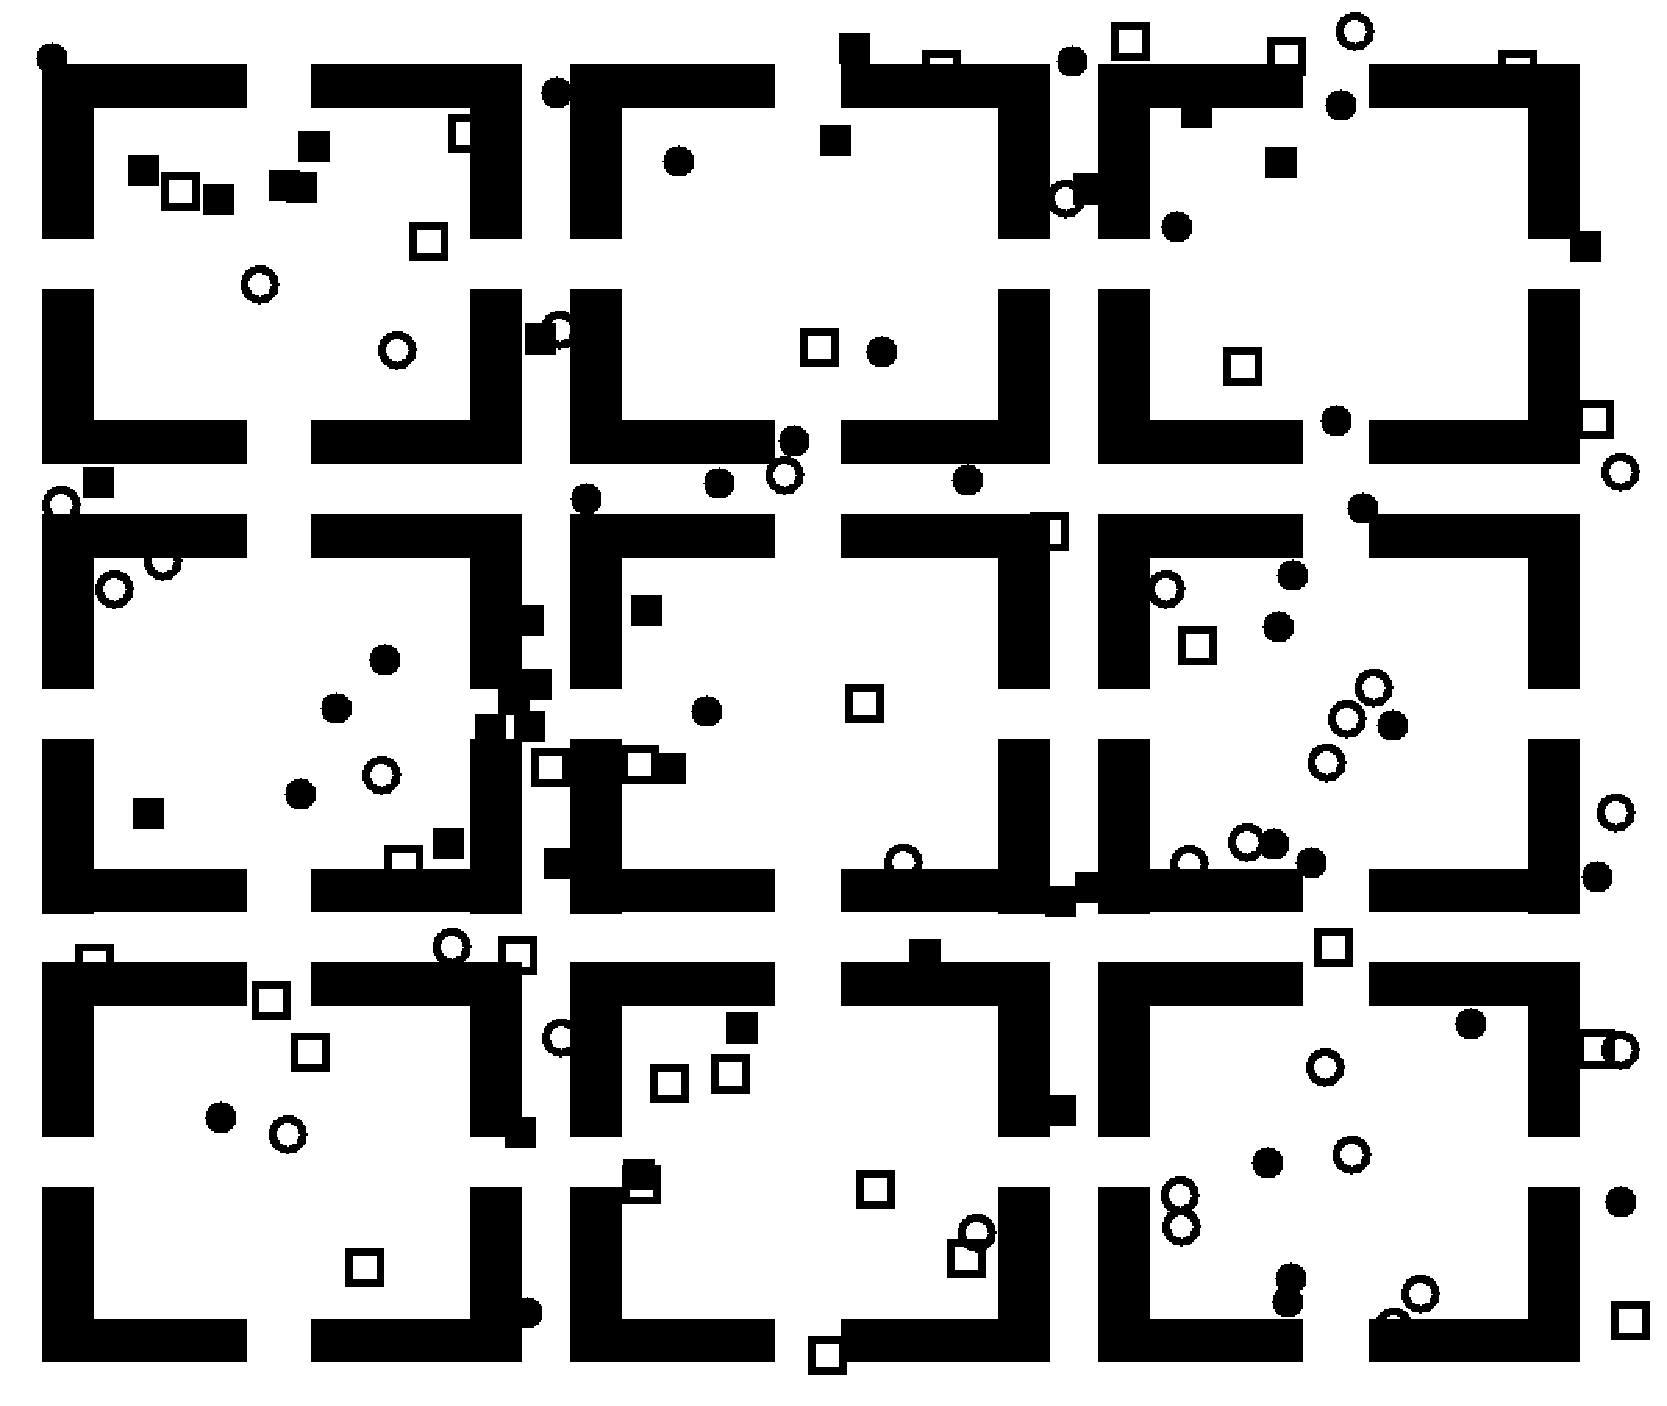
\includegraphics[width=0.3\columnwidth]{img/jos-snapshots/4-1}
    \includegraphics[width=0.3\columnwidth]{img/jos-snapshots/4-3}
    \includegraphics[width=0.3\columnwidth]{img/jos-snapshots/4-4}
    \caption[Simulation run of indoor steering in \alchemist{}]{A simulation run of the reference exposition: three snapshots of \alchemist{}'s graphic reporting module with this simulation. \label{img:museum-generalmap}}    
\end{center}
\end{figure}

We here present simulations conducted over an exposition, where nine rooms are connected via corridors. 
%
People can express different preferences represented by their shape.

Three snapshots of a first simulation run are reported in \Cref{img:museum-generalmap}. 
%
We here consider four different targets that are located in the four rooms near environment angles.
%
People are initially spread randomly in the museum, as shown in the first snapshot, and they eventually reach the room in which the desired target is hosted, as shown in the last snapshot. 


\Cref{img:museum-generalmap2} shows a simulation experimenting with the effect of crowding in the movement of people.
%
Two groups of people -- denoted with empty and full circles -- with common interests are initially located in two different rooms, as shown in the first snapshot. 
%
The target for the dark visitors is located in the central room of the second row, while the others' is in the right room of the second row.
%
In the simulation, dark visitors reach their target soon because it is nearer, thus forming a crowded area intersecting the shortest path towards the target for the other visitors.
%
Due to this jam the latter visitors choose a different path that is longer but less crowded. 

\begin{figure}
\begin{center}
    \includegraphics[width=0.3\columnwidth]{img/jos-snapshots/2-1}
    \includegraphics[width=0.3\columnwidth]{img/jos-snapshots/2-3}
    \includegraphics[width=0.3\columnwidth]{img/jos-snapshots/2-4}
    \caption[Effect of crowding]{A run showing the effect of crowding: dark visitors occupy a central room, making other visitors moving left to right by a longer, less crowded path \label{img:museum-generalmap2}}    
\end{center}
\end{figure}

Both tests show qualitative effectiveness of the proposed laws, and suggest that our simulation approach can be used for additional experiments focussing on tuning system parameters (factor $k$) or alternative strategies (e.g., diffusing crowd information) to optimise paths to destinations.
%
For instance, in the context of the second case, \Cref{img:jos-graph} shows how factor $k$ can influence the time for (sub)groups of (light) people to reach the destination, by which we can see that even small values of $k$ lead to a significant improvement---which slowly decreases as $k$ grows.

\begin{figure}
\begin{center}
   \includegraphics[width=0.99\columnwidth]{img/jos-graph}
   \vspace{-10pt}\caption[Crowd parameter]{Time units of convergence time with different values of crowd parameter and different percentages of people}\label{img:jos-graph}\vspace{-10pt}
\end{center}
\end{figure}


\chapter{Case study: Self composition}

Services are one of the main actors in pervasive and ubiquitous computing. 
%
Composing services is a big issue in these contexts, providing new applications or high level services.
%
Self-composition is even more challenging.

In literature some surveys and possible solutions have been proposed, but only few of them give concrete proposals for the design, implementation and evaluation of service composition.
%
Moreover the composition of services is solved in a centralised way, solution which hardly deal with the large-scale distributed property of pervasive systems, or the composition is specified by the application developers, preventing the system to use new services that appear at runtime.

In this\levelText{}we frame/situate the problem of self-composition in the framework of pervasive ecosystems, defining what a service is and what composing services means. 
%
We then propose an approach to perform self-composition of services and demonstrate our ideas showing how gradients can be composed with other services. 
%
In particular our discussion focuses on the composition of gradient with services providing local levels of crowd, at the purpose of avoiding path crossing overcrowded areas.
%
This example is modelled in terms of LSAs and eco-laws, that are the basic components of a pervasive ecosystem \cite{sapereecolaws-sac2012}, and preliminary simulations, aimed at validating the approach, are run on top of \alchemist{}.

\section{Self-Composition approaches}
A software service represents a functionality that can be provided on demand in order to create higher level software artefacts, such as applications or higher level services.
%
The notion of service allows applications to be easily developed and to adapt by changing the different services, which the application is composed by, at run-time. 
%
Self-composition of services involves the automatic discovery of new services by composing available ones, the selection of services, the plan to execute them (i.e. services execution order), and the adaptation of the composed service when new requirements appear or a service disappears from the system.

\subsubsection{Service Composition in SOA}
The static character of traditional composition approaches such as orchestration and choreography has been recently challenged by so-called dynamic service composition approaches, involving semantic relations \cite{terBeek:06:ASSCFISFM}, and/or AI planning techniques to generate process automatically based on the specification of a problem \cite{wu2007automatic}. 
%
Their basic goal is to analyse a description of the services to compose and compute a composition satisfying structural/behaviour/ontological compliance of the result of composition as can be deduced from information about the composites.
%
One of the main challenges of these approaches is their limited scalability and the strong requirements they pose on the detail of service description.

\subsubsection{Evolutionary techniques}
Evolutionary approaches such as those based on Genetics Algorithms (GA) have been proposed as well for service composition, such as in \cite{Canfora2005}, motivated by the need of determining the services participating in a composition that satisfies certain QoS constraints, which is known to be a NP-Hard problem.
%
More generally, evolutionary approaches have been used in the field of autonomic computing to establish the set of norms, policies or rules that drive the system to the desired emergent behaviour \cite{Norman2010}.
%
We observe that this approach has a potential for service composition: in the same way as the genetic programming determine the proper execution of functions and their parameters, it could be used to find which services, their order of execution and the parameters that its service should receive. 

\subsubsection{Competition-based approaches}
In order to tackle the potentially high number of different compositions that can arise in an open system, in \cite{Viroli:11:SOACCPS} a mechanism of \emph{coordination reactions} for networked tuple spaces is proposed, showing how it can be applied to support competition and composition in a fully distributed setting---services opportunistically compose in those regions of the network where this results in a more competitive service.
%
While all compositions can possibly take place, thanks to a positive/negative feedback only successful ones are meant to ``survive'' in the system, the others fading until becoming never actually selected.
%
This is achieved by matching services with requests through a self-regulating dynamics inspired by prey-predator model of population dynamics \cite{Berryman:1992}, and by diffusing service tuples using a computational-field approach similar to the one presented in \cite{tota-aamas2005,proto}.



\section{A comprehensive approach for pervasive ecosystems}

As previously emphasised, the issue of service composition is becoming wider and wider, and is now encompassing new research areas.
%
Among them -- pervasive computing, autonomic computing, robotics -- we here focus on pervasive computing, and in particular, on the framework of pervasive ecosystems \cite{ecosystems-jpcc7}.
%
There, we understand and design a very large and dense pervasive computing system as a sort of substrate in which humans, institutions, software systems and devices, inject services of various kinds without an a-priori knowledge of the structure and behaviour of those already available and those that will be injected later.
%
Such services diffuse in the network, and are situated and context-aware in the sense that they contextualise to (i.e., they will affect and be affected by) the situation in each \emph{niche} of it.
%
In turn, while in standard SOA a service is a centralised point of functionality, interacting with its clients by stateful protocols of message-passing actions, a service is here a more generalised concept: it is any activity, triggered by the intention of some localised software agent, that flows in the system updating the spatial and temporal configuration of other services, and generating a set of events ultimately perceived by the other agents in the system.
%
Examples of such services include: the materialisation of data produced by all sensors available around, routing services able to interconnect devices based on their physic	al, logical or social proximity, local/global advertisers of the availability of some content, situation recommenders capturing relevant information about a context, and so on.
%
Typical application scenarios include pervasive display ecosystems, augmented social reality, and traffic control---the reader is deferred to \cite{ecosystems-jpcc7} for a more deeper description of them.

\section{The self-composition issue in pervasive service ecosystems}

Pervasive ecosystems naturally call for a radical shift in the way software is designed and developed. The concept of ``software system'' loses its standard meaning of a monolitically designed/implemented/deployed artefact.
%
It is rather a mash-up of services, and the development of a ``new software system'' simply translates into the development of additional services to be immersed in a scenario of existing ones, with the goal of composing with them and evolving their functionalities, thus making software live in a sort of ``eternal beta'' state \cite{Kazman2009}.

The natural questions we have to answer in order to support this vision are hence: what can make services compose if they were not explicitly designed to do so?
%
How can we decide ``whether'' and ``how'' two or more services should compose?
%
How can such decisions be continuously reconsidered depending on the actual (spatial/temporal context) in which the composition is deployed?
%
Can we make multi-level composition seemingly work as well?

We refer to this problem as the self-composition problem for service ecosystems, where by ``self-'' we mean that the underlying middleware makes sure that services tend to compose in order to form meaningful new services, in a way that users of the ecosystems simply perceive only atomic and composite services that are actually useful in practice.

We argue that this vision cannot be fulfilled by the above-mentioned approaches taken in isolation, but instead require them to work altogether.
%
Advanced (semantic) matching of services is key to decide whether two services deployed by third parties can be composed together.
%
Evolutionary approaches seem the only solution to the problem of finely tuning the parameters used in the composition, preselecting, for instance, a subset of more promising compositions. 
%
And finally, competition of different compositions based on their actual exploitation appears instead as the only viable approach to measure the quality of a composition, hence promoting successful ones.
%
On the other hand, understanding how they can work together in a comprehensive framework is very difficult, and generally depends on the specific platform and service model one adopts.

\subsection{Self-Composition with Gradient service}
\label{sec:gradcomp}
To ground our discussion of requirements and possible solutions, we here outline a paradigmatic example of composition in service ecosystems.
%
We consider a crowd steering scenario, based on the idea of guiding people towards locations hosting events of interest in a complex and dynamic environment (using semantic matching with people's interests) without any supervision, namely, in a self-organised way.
%
In particular, we consider a museum with a set of rooms connected by corridors, whose floor is covered with a network of computational devices (called sensor nodes).
%
These devices exchange information with each other based on proximity, have sensors of various kinds, and hold information as LSAs (e.g., about exhibits currently active in the museum).
%
Visitors exploring the museum are equipped with a smartphone device that holds their preferences. By interaction with sensor nodes, a visitor can be guided towards rooms with a target matching his/her interest, thanks to signs dynamically appearing on the smartphone or on public displays. 
%
This system is based on a gradient service, a key brick of self-organisation mechanisms (see \Cref{fig:patterns}) that is typically designed to provide optimal paths to roam a distributed system even in the context of very articulated environments (a building with rooms and corridors, or a traffic scenario) and by dynamically adapting (namely, self-healing) to unpredicted situations such as sudden road interruption \cite{FDMVA-NACO2012,biocore}.
%
Gradient starts from a source LSA located at an exhibition and spreads clones of it to all the nodes of the network by eco-laws of spreading and aggregation, basic building patterns as shown in \Cref{fig:patterns}.
%
In turn, as the gradient is stabilised, in each node the minimum distance value is kept, so that the shortest path to the source is automatically (and dynamically) defined \cite{mass2011}.
%
In this way, a person willing to reach a point of interest simply ``binds'' to a gradient LSA, and public/private displays show signs to guide her to the source.

However, other services exist in the system, such as those provided by the many sensors available around.
%
Among them we have the crowd detection service, enacted by the injection in each node on the floor of a crowd LSA reporting the crowd level sensed there ($0$ is no crowd, $1$ is maximum crowd).
%
An other service is the one that, given visitor preferences and profile, defines a set of other possible points (exhibitions, toilets, refresh points) the user can found interesting or useful.
%
This service can be an external agent that is able to process visitor information, for instance defining related exhibitions, so as to provide, in the form of an LSA, a list of best points the user can pass by.
%
Then we can have sensors for temperature, sensors for pollution, accelerometers etc. 
%
More generally, being a pervasive system an open system, new services may appear in the system, and autonomously be composed with existing ones, without a predefined schema.
%
Only those compositions that create useful services will then survive.
%
To exemplify the idea, in the following we describe two self-composition problem we envisioned.

\subsubsection{Crowd composition}
This self-composition problem focuses on making the gradient service automatically compose to the crowd detection service so that the estimated distance to the source gets ``penalised'' in  case of a high crowd value, which implies that the path computed towards a point of interest intrinsically takes into account situations of crowded areas dynamically emerging in the environment, properly circumventing them.
%
In particular what we expect to the middleware to automatically do is: decide to compose the gradient with crowd sensing instead of with other (irrelevant sensors), and optimally tune how much crowd information should affect the computation of optimal path.

\subsubsection{Ad-hoc path composition}
If the gradient service is tagged with the point of interests crossed, it can be composed with the list of  ``best points'' defined for each user, so that, in case of intersection, such gradient gets ``reinforced" for instance diminishing its value, which then implies that the direction it comes from has more chance to be chosen, and paths which cross points interesting or useful for the user are likely to be followed. 
%
In particular what we expect to the middleware to automatically do is: decide to compose the gradient with the LSA representing the ``best points", and optimally tune to which extent information on preferences should affect the computation of optimal path. 

\subsection{A prototype solution}
Starting from a number of services available in those nodes where sources of gradient services are located -- all reified by an LSA that can be injected in different parts of the system but via chemotaxis reach gradient sources -- the solution we propose is based on the following mechanisms:

\subsubsection{Composition}
Based on one or more ``composition recommender'' agents available in source nodes, all the available compositions are computed using techniques of advanced matching of interface/behaviour/ontology. These are ranked -- according for instance to feedbacks  from the users on the composite service, as discussed later --  and the description of a limited number of them is reified in the space in the form of a set of LSAs. 
%
In the example of crowd steering proposed above, these compositions should result in a set of LSAs representing the source of different gradients, each one created composing the basic gradient with one or more services. We assume that the composition actuated, \emph{i.e.} which services are composed and which parameters are used in the composition, is stored into a property of the gradient LSA, so that the same composition can be performed in all the locations of the system.

\subsubsection{Contextualisation}
From the source, composite gradients and the basic one, are diffused. In each location they are contextualised with the local value of those services they are composed by. 
%
Contextualisations involving gradients normally result in a modification of the local value of distance according to a function $\delta$ specified in the service or defined by the composition agent. 
%
If services are not locally available, contextualisation does not happen and the distance value does not change. 
%
For instance, contextualise gradient  with the crowd level perceived in each location at the purpose of discouraging paths crossing crowded areas. It means that distance should be increased and function $\delta$  looks like $\delta = k * c$ where $k$ is a function parameter (see later how to define its values), and $c$ is the local crowd level. 

\subsubsection{Choice}
The resulting effect is that the gradient service is available in the system in different forms (the basic one and the composite ones), and users, once entering in the system, can probabilistically choose among them, grounding such decision mainly on the distance and satisfaction values.
%
They will then follow the same composition for the whole path.

\subsubsection{Feedback}
Each gradient owns a property called ``satisfaction'', representing the feedback of users on the quality of the service itself.
%
It can for instance evaluate the length of the path, the interest  and so on: the higher the value is, the higher is the user satisfaction. 
%
People, once they reach the source, should then provide their feedbacks in the form of  LSAs with predefined properties ---such as length, comfort, beauty, interest.
%
Marks, for each property, might be defined in a predefined range. 
%
From there one agent can then be in charge to compute the satisfaction value as a function of all the marks given -- for instance, the average.
%
The LSA of the correspondent gradient source is then modified by adding to the previous value of the satisfaction property the last computed.
%
This updated value is then spread  in the whole system autonomously as a result of gradient diffusion.
 
\subsubsection{Evaporation}
The satisfaction value can also be interpreted as the relevance value of the Evaporation pattern \cite{FDMVA-NACO2012}.
%
This parameter gets decreased until fading if not augmented by user positive feedbacks. Once it is equal to zero the composite service can be removed. This mechanism ensures that no satisfactory compositions are decayed.

\subsubsection{Evolution}
If parameters are to be chosen for the composition -- for instance parameter $k$ in $\delta = k * c$, representing how much the crowd level has to influence the distance value of the field --, they can be tuned by agents implementing evolutionary techniques.
%
They are in charge to define the  new population of parameters according to the fitness function that can be computed from the satisfaction value of the gradient itself.

\noindent The emergent idea is that, after a transition period, system makes available only those services that better fit user preferences. For instance, for those users interested in quickly reach the sources, only those gradients that ensure the lowest arrival time should survive.


\section{A formal model for gradients self-compositions}
To describe how self-composition of gradients can be built in the SAPERE framework, we first introduce the implementation schema for gradients which we shall rely upon to formalise the self-composition task in the specific example of crowd service exploitation.

\subsection{The gradient service}
Our strategy for modelling gradient's features: 
\begin{enumerate}
 \item a continuous broadcast of information in each node as in \cite{flexiblegradients}, with latter information always overwriting previous one;
 \item propagation of estimated distance, computed by summing the contributions given by property \texttt{mid:distance} in neighbour annotation;
 \item propagation with no horizon (it is easy to impose a distance bound to the propagation of information);
 \item after been sent to a neighbour, an annotation is subject to a contextualisation phase (in which e.g. aggregations are executed) before being spread again.
\end{enumerate}

\begin{figure}\vspace{10pt}
{\footnotesize
\begin{Verbatim}[samepage=true, frame=single, commandchars=\\\{\}, label={\small \bf Transition Rules for Gradients}]
# [PUMP] An annotation of type source continuously injects the initial
# gradient annotation
\textbf{?SOURCE} sos:type sos:source; sos:aggr_prop ?P; sos:step ?T;
     sos:r_diff ?R; sos:r_ctx ?RC
--?R--> 
\textbf{?SOURCE} sos:step =(?T+1) +
\textbf{?GRAD}(?GRAD clones ?SOURCE) sos:type -sos:source sos:diff
     sos:aggr; sos:dist "0"; sos:orientation "here"

# [DIFF] A gradient annotation is cloned in a neighbour, with distance
# increased and updated orientation
\textbf{?GRAD} sos:type sos:diff; sos:dist ?D; sos:r_diff ?R +
\textbf{?NEIGH} mid:type mid:#neigh; mid:remote ?L; mid:orientation ?O;
     mid:distance ?D2
--?R-->
\textbf{?GRAD} + \textbf{?NEIGH} +
\textbf{?GRAD1}(?GRAD1 clones ?GRAD)  sos:type -sos:diff sos:ctx;
     sos:dist=(?D+?D2); sos:orientation =?O; mid:#loc ?L

# [CTX] A contextualising annotation is transformed back into an annotation
# to be diffused
\textbf{?GRAD} sos:type sos:ctx; sos:r_ctx ?RC
--?RC->
\textbf{?GRAD} sos:type sos:-ctx sos:diff;

# [YOUNGEST] Of two annotations to be aggregated based on property ?P, the
# one with newest information is kept
\textbf{?ANN1} sos:type sos:aggr; sos:aggr_prop ?P; ?P =[?C]; sos:step ?T +
\textbf{?ANN2} sos:type sos:aggr; sos:aggr_prop ?P2; ?P2 =[?C]; sos:step ?T2(?T2<?T)
--->
\textbf{?ANN1}

# [SHORTEST] Of two annotations to be aggregated based on property ?P,
# the one with shortest distance from source is  kept
\textbf{?ANN1} sos:type sos:aggr; sos:aggr_prop ?P; ?P =[?C]; sos:dist ?D1;
     sos:step ?T  +
\textbf{?ANN2} sos:type sos:aggr; sos:aggr_prop ?P2; ?P2 =[?C];
     sos:dist ?D2(?D2>=?D1); sos:step ?T
--->
\textbf{?ANN1}

[DECAY] An annotation decays
\textbf{?GRA} sos:type sos:diff; sos:r_dec ?RD
--?RD->

\end{Verbatim}
}
\vspace{-10pt}\caption{Rules for gradients}\label{laws:gradient}
\end{figure}

Such rules are reported in \Cref{laws:gradient} and are described in turn.
%
Note that they refer to namespace \texttt{mid} for URIs related to middleware activities, and to \texttt{sos} for those concerning self-organisation aspects.

Rule [PUMP] is a transformation rule which takes a source annotation and creates a new annotation with distance set to $0$, used to start the spreading process.
%
The source annotation should feature property \texttt{sos:type} assigned to value \texttt{sos:source} (we shall say the annotation is of type \texttt{source} for brevity), and it should also have some value assigned to properties \texttt{sos:aggr\_prop} (the name of the property holding the value used to aggregate other annotations as described below), \texttt{sos:step} (an incremental value used to refresh information), \texttt{sos:r\_diff} (diffusion rate) and \texttt{sos:r\_ctx} (contextualisation rate).
%
This rules fires at diffusion rate \texttt{?R}: according to CTMC semantics, this means that as soon as a matching set of reactant annotations is found, actual application of the rule is delayed of a time $t$ randomly drawn according to a negative exponential distribution of probability with average value $1/\texttt{?R}$---namely, it is fired at frequency \texttt{?R}.
%
The effect of firing this rule is twofold: it increases the value of property \texttt{sos:step} of the source annotation, and creates (by cloning the source) a new annotation \texttt{?GRAD} of type \texttt{sos:diff} and \texttt{sos:aggr} (original type \texttt{sos:source} is removed), and declaring distance $0$ and orientation \texttt{here} with respect to the source---these properties will be update as the annotation is spread around.
%
Note that the right-hand side of a rule mentions only changes in annotations, without any need of repeating information provided in the left-hand side which has not changed: this allows a simpler structuring of rules with respect to more syntactic approaches like the one in \cite{mass2011}.

Rule [DIFF] is used to diffuse a cloned version \texttt{?GRAD1} of a gradient annotation \texttt{?GRAD} in one neighbour.
%
The gradient annotation should be of type \texttt{diff}, declare distance \texttt{?D} from the source and have diffusion rate \texttt{?R}.
%
This rule has as further reactant a neighbour annotation, from which information about a neighbour \texttt{?L} with orientation \texttt{?O} and distance \texttt{?D2} can be extracted.
%
This rule leaves the reactants unchanged, but creates a clone of \texttt{?GRAD} with type \texttt{ctx} instead of \texttt{diff}, to be relocated at \texttt{?L} and indicating orientation (with respect to originating location) \texttt{?O} and distance \texttt{?D+?D2}.
%
Note that continuous application of this rule at rate \texttt{?R} makes copies of the gradient annotation to be created and diffused in all neighbours.

An annotation is relocated with type \texttt{ctx}, which forbids further application of rule [DIFF].
%
This is because we first need to aggregate all incoming annotations before a new diffusion is scheduled.
%
To do so, rule [CTX] defers change of type from \texttt{ctx} to \texttt{diff}, which happens at rate \texttt{?RC} (contextualisation rate).

One form of aggregation is due to rule [YOUNGEST], used to refresh gradients with new information.
%
It takes two annotations such that the values associated to the aggregation property \texttt{?P} are the same, and retains the one with bigger \texttt{sos:step}.
%
The idea is that \texttt{sos:aggr\_prop} holds the name of a property \texttt{?P} which is expected to contain some value(s) that should be identical in two annotations for them to be aggregated.
%
For instance, it could be the unique id of a gradient source, so that we do not aggregate annotations coming from difference sources---but more involved situations can be programmed as exemplified in next section.

Rule [SHORTEST] is similar: it takes two annotations with same step (hence coming from the same gradient annotation as generated by rule [PUMP]), and retains the one with shortest distance only if, again, they have same content of aggregation property.

Finally, rule [DECAY] is used to remove an annotation at a given decay rate \texttt{?RD}. This is useful as a cleanup mechanism in the case a gradient source is removed from the system---though it plays no crucial role in and will be neglected in next discussions.

For the above rules to properly work we need to synthesise a well-structured source annotation, featuring all required properties and proper values for rates---namely, diffusion rate is to be chosen to keep the system sufficiently reactive to changes without bloating the system with undesired messages, and contextualisation rate should be significantly higher than diffusion rate (at least one order of magnitude).
%
For instance we could use the following source annotation:

{\begin{verbatim}
:id314 mid:#loc :loc117;  sos:type sos:source; 
       sos:step "0";      sos:sourceid "341AB2"
       sos:aggr_prop sos:sourceid; 
       sos:r_diff "10";   sos:r_ctx "100"
\end{verbatim}}



\subsection{Rules for Gradient Composition}

\begin{figure*}[t!]\vspace{10pt}
{\footnotesize \begin{Verbatim}[frame=single, commandchars=\\\{\}, label={\small \bf Eco-laws for gradient contextualisation}]
# [COMPOSITION] The gradient source is composed with the crowd service
\textbf{?SOURCE} sos:type sos:source; scm:satisfaction ?S +
\textbf{?CROWD} scm:type crowd; crowd:level ?CL 
---> 
\textbf{?SOURCE} +
\textbf{?CSOURCE}(?CSOURCE clones ?SOURCE) scm:property sos:dist;
     scm:parameters scm:crowd_op  ?CF;  scm:crowd_op  ?CF*?CL

# [CONTEXTUALISATION] If sensors perceive crowd, the gradient distance is
# augmented
\textbf{?GRAD} sos:type sos ctx; sos:dist ?D;  scm:property sos:dist; 
     scm:parameters scm:crowd_op scm:crowd_factor; scm:crowd_factor ?CF;
     scm:crowd_op  ?CF*?CL +
\textbf{?CROWD} scm:type crowd;  crowd:level ?CL 
--->
\textbf{?CROWD} + \textbf{?GRAD}  sos:type -sos:ctx sos:diff; sos:dist =(?D+?CF*?CL)

# [FEEDBACK] Feedbacks are used to update the satisfaction values
\textbf{?FEEDBACK} scm:parameters scm:crowd_op; scm:feedback  scm:velocity;
scm:velocity ?V +
\textbf{?GRAD} scm:satisfaction ?S; scm:parameters scm:crowd_op 
--->
\textbf{?GRAD} scm:satisfaction =(?S+?V)

# [EVAPORATION] The gradient satisfaction value gets decreased
\textbf{?GRAD} scm:satisfaction ?S; scm:factor_ev ?FE; scm:r_ev ?RE
--?RE->
\textbf{?GRAD} scm:satisfaction =(?FE*?S)

# [DECAY] If the gradient satisfaction value becomes zero that composition
# is removed
\textbf{?GRAD} scm:satisfaction "0"; 
--->

\end{Verbatim}
}
\vspace{-10pt}\caption{Additional rules for anticipative gradients.}\label{laws:crowd}
\end{figure*}

%
Rule [COMPOSITION] in \Cref{laws:crowd}, is in charge of creating the source of the composite gradient. The new source owns the same set of properties of the basic one, as soon as it refers to the same PoI, but it also defines which properties are to be modified as an effect of the composition  -- \texttt{sos:dist} --, and which are composition parameters -- \texttt{scm:parameters} -- , \emph{i.e.}  function -- \texttt{scm:crowd\_op} -- to be used for modifying the distance value, and coefficient ---\texttt{scm:crowd\_factor}. In this preliminary example we adopt a simple linear function of the crowd level perceived by sensors in each location. It increases the distance of those paths crossing crowded area, if the coefficient has an opportune value.
%
Rule [CONTEXTUALISATION]  applies the composition specified in \texttt{scm:parameters}, in each location of the system.
%
Rule [FEEDBACK] is used to modify the satisfaction value of gradient, taking into account the velocity of the path chosen. It can be computed by the system itself, or provided by the user. The value of \texttt{scm:satisfaction} gets increased by \texttt{scm:velocity} value.

Rules [EVAPORATION] and [DECAY] are finally used to evaporate the \texttt{scm:satisfaction} value according to an evaporation factor \texttt{scm:factor\_ev ?FE} in the range of [0,1] and to remove the gradient composition in case of a \texttt{scm:satisfaction} value equal to zero, or negative, ensuring that only those compositions that compute fast paths will survive.

\section{Towards simulation of gradient self-compositions}

We checked the correctness of the proposed self-composition solution by simulation, conducted using \alchemist{}.

Results presented show early experiments on gradient composition with crowd level, where people dynamically enter in the system and begin to move towards the target ascending one of the different compositions available. Movement velocity is constant in the system, except for crowded areas, where it decreases according to the crowd level perceived: higher crowd, slower velocity.
%
In these early experiments, parameter $k$ in function $\delta$ is not computed dynamically through an evolutionary algorithm but composition agents define a set of possible values. A new composition corresponds at each value.
%
Users chose one gradients randomly but considering also the associated satisfaction value  that measures the velocity of the best path each gradient proposes. This feedback is computed by each user once reached the target, given the length of the path and the distance walked.

The goal is to observe that, satisfaction values, initially the same for each composition, dynamically change according to feedbacks from the users, and only best compositions survive. In \Cref{fig:scsimu} such process is shown for different values of parameter $k$: the system reaches a stable state with $k=0.5$ ensuring the faster path while the other compositions decay.

\begin{figure}
	\begin{center}
 		\includegraphics[width=\textwidth]{img/sc-simu.pdf}
\end{center}
\caption{Satisfaction values for different compositions changing over time.}
\label{fig:scsimu} 
\end{figure}

\chapter{Case study: Semantic resource discovery}

Supporting expressive resource discovery atop this unstructured, highly-dynamic substrate presents a challenge, with the combination of semantic reasoning, context-awareness and self-organisation techniques offering intriguing possibilities: semantic matching provides a flexible framework for quantitatively assessing the suitability of resources to a given request; context-awareness may account for application quality of service concerns that are important, but orthogonal to the matching process, and self-organisation techniques provide a means of adapting to changing environmental conditions---the arrival and removal or resources, the mobility of interacting agents, and the ever evolving network topology.

To illustrate the utility of this approach, we consider a smartphone application for an exhibition centre (for example, Tokyo's Makuhari Messe, which contains eleven exhibition halls and has a footprint of $210,000m^2$), which offers routing information and exhibit suggestions based on a user's profiled interests. These techniques support the development of exploration strategies to:
\begin{itemize}
 \item select the exhibit most suited to the user's interests;
 \item select preferential exhibits while accounting for factors such as their distance from the user's position or crowdedness along the route;
 \item route the user to an exhibition hall containing many exhibits of interest, but not necessarily the most interesting if it is considered spatially isolated;
 \item use a combination of the above strategies, for example, to guide the user to a particular exhibition hall and then route them to the exhibits inside the hall in order of interest or least crowded.
\end{itemize}

\section{Semantic Matching in SAPERE}
\label{sec:semantic_matching}
\begin{table}
\centering
%\begin{small}
\begin{tabular}{| c || p{6cm} | c | c |}\hline
\textbf{Match Degree}        &\textbf{Description}	&\textbf{DL Notation}  &\textbf{Similarity (R, A)} \\\hline
\emph{Exact}	&The request and advertisement are equivalent concepts.	&$R \equiv A$	&1		\\\hline
\emph{Subsume}	&The request expresses a more general concept than the advertisement.	&$A \sqsubseteq R$	&1		\\\hline
\emph{Plugin}	&The request expresses a more specific concept than the advertisement.	&$R \sqsubseteq A$	&$\frac{|S(A)|}{|S(R)|}$		\\\hline
\emph{Intersection}	&The intersection of the request and advertisement is satisfiable.	&$\neg (R \sqcap A \sqsubseteq \perp)$	&$\frac{|S(A)\sqcap S(R)|}{|S(R)|}$		\\\hline
\emph{Disjoint}	&The request cannot be satisfied by the advertisement.	&$R \sqcap A \sqsubseteq \perp$	&0		\\\hline
\end{tabular}
%\end{small}
\caption[Match-degrees and their semantic scores]{Match-degrees and their semantic scores, defined using the similarity metric proposed by Skoutas et al.~\cite{skoutas2007raking}. $S(X)$ denotes the set of super-concepts of concept $X$ in its defining ontology.}
\vspace{-10pt}
\label{tab:match_degrees}
\end{table}

\subsection{Semantic Matching}
A matchmaking process takes a request and a set of resource descriptions as input, and outputs the set of resources that satisfy the request.
%
Many matchmakers adopt simple syntactic schemes; for example, named interfaces or predefined categories~\cite{waldo2000jini}, or sets of attribute-value pairs to which string and numeric comparisons can be applied~\cite{guttman1999service}.
%
Such approaches are limited by an inability to compare semantically equivalent but syntactically different concepts or handle approximation.
%
To illustrate, consider the concept hierarchy depicted in \Cref{fig:concept_hierarchy}, based on the Vehicle Sales Ontology\footnote{\url{http://www.heppnetz.de/ontologies/vso/ns}}.
%
Here, the concepts  \texttt{Automobile} and \texttt{Car} may be considered as equivalent terms, or \texttt{TwoDoorCar} as an approximate match to a \texttt{FourDoorCar}.
%
Semantic analysis supports the incorporation of such matches where they would otherwise be discounted.

A semantic matching process has three parts: a model for describing requests and resources, a scheme for measuring the semantic similarity of concepts, and an algorithm for evaluating the match.

\subsubsection{Modelling Resources and Requests}
A request expresses the intersection of a number of properties, each named concept or existential restriction belonging to a resource. Using Description Logics (DL) notation~\cite{baader2003description}, the following describes a request for two door, electric cars manufactured after 2009, and three advertisements for candidate vehicles to be matched against this request. 

\begin{samepage}
\noindent {
$R$: $TwoDoorCar$ $\sqcap$ $ \exists modelDate \geq 2009 $ $\sqcap$ $\exists fuelType=Electric$\\
$A1$: $Automobile$ $\sqcap$ $ modelDate=2009$ $\sqcap$ $ fuelType=Hybrid$\\
$A2$: $TwoDoorCar$ $\sqcap$ $ modelDate=2011$ $\sqcap$ $ fuelType=Petrol$\\
$A3$: $Van$ $\sqcap$ $ modelDate=2011$ $\sqcap$ $ fuelType=Electric$\\
$A4$: $Bicycle$ $\sqcap$ $ modelDate=2007$
}
\end{samepage}
\begin{figure}
\centering
\includegraphics[width=\columnwidth]{img/concept_hierarchy}

\caption[Partial illustration of concepts in the Vehicle Sales Ontology]{A partial illustration of concepts in the Vehicle Sales Ontology, an equivalence relation from one term to another concept hierarchy, and a snippet from a fuel type ontology.} 
\label{fig:concept_hierarchy}
\end{figure}

None of the four advertisements fully satisfies the request: there is insufficient information to determine if $A1$ is a $TwoDoorCar$; $A2$ differs in the requested fuel type; although electric, $A3$ is a Van; and $A4$ satisfies no request aspects.
%
However, by inspection we can see that some of the advertisements more closely relate to the request than the others.
%
We say that an advertisement is \emph{compatible} with a request if the intersection of their descriptions is satisfiable.

\subsubsection{Quantifying Semantic Similarity}
\label{ref:quantifying}
\cite{paolucci2002semantic} and \cite{li2003software} introduce ordered degrees of matching to categorise the semantic compatibility between a request ($R$) and an advertisement ($A$), of which there are five: \emph{exact}, \emph{plugin}, \emph{subsume}, \emph{intersection}, and \emph{disjoint}.
%
\cite{bandara2008semantic} extends this model with scoring mechanisms to support differentiation of matches falling within the same category.
%
Descriptions of the match-degrees and formulas for scoring taxonomically related concepts are shown in \Cref{tab:match_degrees}.

Applying this mechanism to the concept hierarchy in \Cref{fig:concept_hierarchy} allows us to quantify the similarity between terms in our earlier example.
%
For example, the degree of similarity between $Automobile$ and $TwoDoorCar$ is $0.75$ (plugin), the degree of similarity between $TwoDoorCar$ and $Van$ is $0.5$ (intersection), and the degree of similarity between $Hybrid$ and $Electric$ is $1$ (subsumption).

\subsubsection{Executing the Semantic Match}
\label{sec:match_algorithm}
A semantic matching algorithm conflates all the terms in a request and resource description and may be realised in many ways.

A possible implementation of a \texttt{MATCH} algorithm takes two variables $R$ and $A$ as input, which correspond to the request and advertisement or some sub-set of their terms respectively.
%
The function first checks if $R$ subsumes $A$; if so, the algorithm terminates with a similarity score of 1.
%
If $R$ and $A$ refer to atomic named concepts or literals, the similarity score is calculated by a call to the \texttt{SIMILARITY} function, which resolves the comparison to a score depending on how the concepts are related.
%
If not, $R$ and $A$ are composites consisting of named concepts or existential restrictions.
%
This case is handled by recursively decomposing $R$ into its constituent parts, $R_{1..n}$, and averaging the maximum score for each $R_i$, when compared with corresponding parts of $A$, that is, $A_{1..m}$.
%
Applying this algorithm to the above example yields the scores: $A1$=$.92$, $A2$=$.83$, $A3$=$.83$, and $A4$=$.08$.

\section{Distributed Resource Discovery}
\label{sec:operational_framework}
We now clarify how standard self-organisation patterns can be augmented with semantic reasoning so as to support a decentralised approach to resource discovery in pervasive computing applications.

\subsection{Self-organisation Patterns}
This section briefly reviews those patters that form our interaction building blocks.

\subsubsection{Spreading}
The Spreading pattern progressively sends information over the system from one node to its neighbourhood, iteratively, so as to make it available globally by using only local interactions.
%
In our framework it is supported by the following eco-law:
%
\begin{Verbatim}[samepage=true, frame=single, commandchars=\\\{\}, label={\small \bf Spreading}]
?A :val ?V; :diff ?F; :loc ?L
--> 
?A + ?B :#clones ?A; :val =?W; :loc ="*"; :prev = ?L
?BIND (:exec2(?F,?V) AS ?W)
\end{Verbatim}

\subsubsection{Aggregation}
The Aggregation pattern reduces the amount of information in the system, typically by summarising data disseminated by agents over time, e.g., by spreading.
%
It is supported by:
%
\begin{Verbatim}[samepage=true, frame=single, commandchars=\\\{\}, label={\small \bf Aggregation}]
?A :src ?S; :aggr ?F; :val ?V + ?B :src ?S; :val ?W 
--> 
?A :val =?Z :
?BIND (:exec3(?F,?V,?W) AS ?Z)
\end{Verbatim}

\subsubsection{Decay}
The Decay pattern incrementally ages information in the system.
%
A monotonically decreasing function is applied to a numeric decay value over time, with the information removed upon the counter reaching zero.
%
Decay-based Aggregation supports the overwriting of old information from a data source with the more recent.
%
Decay is supported by the following eco-laws:
%
\begin{Verbatim}[samepage=true, frame=single, commandchars=\\\{\}, label={\small \bf Decay}]
?A :decay ?D :dfunc ?F;
--> 
?A :decay ?N;
?BIND (:exec4(?F,?D) AS ?N)

?A :decay 0;
--> 
\end{Verbatim}

\subsubsection{Gradient}
The Gradient pattern is a composition of the Spreading and Aggregation patterns, where information about the sender distance and direction is propagated across an extent of the network.
%
An LSA can become source of a gradient by specifying initial distance $0$, a diffusion function incrementing the distance value, and an aggregation function retaining the less traveled LSA among competing gradient LSAs from the same source \cite{sapereecolaws-sac2012}.
%
The Decay pattern supports \emph{dynamic} gradients by discarding old information as a gradient source moves within the network.

\subsubsection{Chemotaxis}
The Chemotaxis pattern provides a mechanism to route information towards the source of a gradient via the shortest accessible path.
%
In our framework, movement of LSAs towards a gradient source is achieved by diffusing in the direction indicated by property \texttt{:prev} as created by the Spreading eco-law.

\subsection{Self-organising, Context- and Semantics-aware Resource Discovery}
\begin{figure}
\centering
\includegraphics[width=\columnwidth]{img/newprocess}
\caption[Resource discovery interactions]{Resource discovery interactions: (A) a request gradient is spread, and (B) replies ascend the gradient and aggregate.} 
\label{fig:distributed_interaction}
\end{figure}

Building upon the above concepts, we now introduce the key steps in our approach to self-organising, context- and semantics-aware resource discovery, which are illustrated in \Cref{fig:distributed_interaction}.

\subsubsection{Establish the resource request}
An application searching for a resource publishes a \texttt{request} gradient LSA carrying information about the source $R$ of the request: spreading and aggregation eco-laws will iteratively fire in random establishing a gradient data structure, with horizon $H$ (hop distance counter), and  in which each LSA has a pointer to the node in which it was created, which is also the node indicating direction to the source following shortest path.

\subsubsection{Resolve matches and publish reply}
Where a gradient LSA containing a request is co-located with an annotation describing a resource (or service) $S$, we apply semantic matching, as described in \Cref{sec:semantic_matching} to resolve their compatibility to a match-degree.
%
This is realised by a matching eco-law that creates a \texttt{reply} LSA pointing towards the request and the service, and with the value $MD$ representing the match-degree (greater than $0$). 

\subsubsection{Route match information to the requestor}
The reply LSA is created such that it diffuses by copying towards the request source; namely, the chemotaxis pattern is applied to deliver a remote representation of the resource annotation matched to the request source. This is continually applied to maintain a live link between the two points in the network: the request site and service site.
%
This ends after the request gradient expires, for example, after the request is explicitly removed.
%
This allows the process to update and self-heal under conditions where:
\begin{itemize}
 \item an intermediate node used for routing fails;
 \item a compatible resource appears within the gradient;
 \item the requestor or resources are mobile within the network.
\end{itemize}

\subsubsection{Augmenting matches with application context}
As the reply LSA is routed, aggregation may be employed to modify, either positively or negatively, the reported match-degree, using information external to the reply.
%
This is achieved by applying an aggregation function to any LSA directed towards a request source that accounts for contextual factors (\emph{any information that can be used to characterise the situation of entities that are considered relevant to the interaction}~\cite{dey2001conceptual}) specified by the application; and with such information readily available for consumption through its expression in an LSA.
%
For example, $\lsa{S_0, 0.9, 0.75}$ (resource, original-match-degree, match-degree) might represent a reply LSA that has been updated to account for the distance an LSA has travelled, or the presence of physically crowded regions along the response path. 

\subsubsection{Aggregate results en route by competition}
Where a request is matched to multiple, distributed resources, the algorithm returns the most suitable to the requestor.
%
For example, in the case where there are two co-located response annotations of the form $\lsa{S_0, 0.9, 0.75}$ and $\lsa{S_1, 0.8, 0.8}$ (resource, original-match-degree, match-degree), the latter will be propagated while the former will be dropped.
%
Combining this with the previous mechanism provides a contextual-semantic approach whereby a resource may be retained that, although it has worse match-degree when considered in isolation, better accounts for a requestor's contextual requirements.

\subsubsection{Aggregate results en route by collaboration}
An alternative to the above approach is to augment the standard semantic-matching process by making a resource more, or less, attractive depending on some contextual relation to similarly matched resources.
%
For instance, in applications where resources represent physical points of interest (POIs), we may consider a small region of the space that includes many POIs more favourable than another region containing the POI with highest match-degree. 
%
This is achieved by an aggregation function that ``joins'' two replies instead of selecting one of them. For example, response annotations of the form $\lsa{S_0, 1 , 0.9}$ and $\lsa{S_1, 2, 0.75}$ (resource, distance, match-degree), can be subject to joining as they represent spatially close services.
%
Hence, they are aggregated into a single annotation $\lsa{S_0+S_1, 1.5 , 0.85}$, in which distance and match-degree summarise the original ones.
%
As before, application specified contextual factors may readily be accounted for.

\subsubsection{Receipt of replies}
The requestor will eventually receive aggregated replies, providing information about (summary) distance, (summary) match-degree, resource provider (or resources provider), and direction to reach the service.
%
Such information can then be used, for example, to steer the requestor agent towards a selected resource or selected resources, as developed in \cite{sapereecolaws-sac2012}.

\subsubsection{Dynamic self-healing}
The evolution of ecosystem states over time is supported by the Decay pattern, which is employed to periodically remove older information while newer information is concurrently refreshed.
%
The periodic update of request gradients and reassertion of responses accounts for the requestor moving closer to or further away from resources, for resources disappearing or arriving, and for the corresponding impact these changes have on the aggregation applied to the match degree results in transit. 


\begin{figure}
{\scriptsize 
\begin{Verbatim}[frame=single, commandchars=\\\{\}, label={\small \bf Resource discovery with match-degree and spatial information}]
% [MATCH] When a request and service match, a reply LSA is generated to be diffused towards
% requestor
?REQ :type :request; :content ?R; :source ?SRC + ?SER :type :service; :content ?S
--?Rate-->
?REQ + ?SER +
?REP :#clones ?REQ; :type = :reply; :service ?SER; :content ?S; :original_match_degree ?MD;
     :match_degree ?MD; :ctxed "false"; sos:direction ?SRC; sos:switcher :ctxed;
     sos:type sos:ascend
BIND(:semanticMatchDegree(?R, ?S) AS ?MD)
FILTER(?MD > 0)
BIND(:replyRate() AS ?Rate)

%[CTX] A reply contextualises, and is accordingly propagated one-step
?REP :type : reply; :ctxed "false"; :ctxprop ?P; :ctxtype ?T; :ctxfun ?F; ?P ?V
?CTX :type ?T; ?P ?V2
--?Rate-->
?REP :ctxed = "true"; ?P = ?W +
?CTX
BIND (:exec(?F,?V,?V2) AS ?W)
BIND(:diffRate() AS ?Rate)

% [AGGREGATE-COOP] Joins information from two replies belonging to the same service cluser
?A1 :type :reply; :ctxed "true"; :request ?R; :service ?S1; :ctxprop ?P; ?P ?V1;
     :match_degree ?MD1; :coop_pred ?CP; :coop_md ?CM; coop_ctx ?CC +
?A2 :type :reply; :ctxed "true"; :request ?R; :service ?S2; :ctxprop ?P; ?P ?V2;
     :match_degree ?MD2
--->
?A1 :service ?S; ?P = ?V; :match_degree = ?MD
FILTER(:exec(?CP,?V1,?V2)) .                    % The two services should "cooperate"
BIND (:exec(?CC,?V1,?V2) AS ?V) .               % Let V be the aggregated contextualisation
BIND (:exec(?CM,?MD1,?MD2) AS ?MD) .            % Let MD be the aggregated match-degree
BIND (:union(?S1,?S2) AS ?S) .                  % Let S the aggregated service description

% [AGGREGATE-CHOOSE] Selects between two replies originating within different service clusters
?A1 :type :reply; :ctxed "true"; :request ?R; :service ?S1; :ctxprop ?P; ?P ?V1;
     :match_degree ?MD1; :comp_pred ?CP; :coop_sel ?CS +
?A2 :type :reply; :ctxed "true"; :request ?R; :service ?S2; :ctxprop ?P; ?P ?V2;
     :match_degree ?MD2
-->
?A :service ?S1; ?P ?V; :match_degree ?MD1
FILTER(:exec(?CP,?V1,?V2)) .                    % The two services should "compete"
FILTER(:exec(?CS,?V1,?MD1,?V2,?MD2)) .          % Service A1 has a stronger match-context pair
\end{Verbatim}
}
\caption{Eco-laws for handling request-reply match, and for distributed aggregation.}
\label{fig:laws}
\end{figure}

\section{Eco-laws to support matching}
\label{sec:ecolaws}
In this section we present eco-laws that support the contextual-semantic management of resource discovery, describing their behaviour and the functions they encapsulate. For the sake of space we will not provide the general-purpose eco-laws supporting the spreading, aggregation, gradient, and chemotaxis self-organisation patterns, for they are discussed elsewhere \cite{sapereecolaws-sac2012}.
%
We instead focus on the four eco-laws that incorporate the key strategies described in previous section, namely, the generation of replies along with a match-degree, their contextualisation at each node they transit across, and the competition-/collaboration-based aggregation as they are routed towards the requestor.
%
They are presented in \Cref{fig:laws}, and described in turn.
%
These eco-laws make use of a default (omitted) name-space corresponding to the ontology of resource discovery, the \texttt{sos} namespace incorporating the concepts relating to self-organisation patterns, and the \texttt{sapere} namespace incorporating all the general concepts of pervasive service ecosystems.

Eco-law \texttt{[MATCH]} creates the reply.
%
It takes a request LSA \texttt{REQ} and a service LSA \texttt{SER} located in the same node, and creates the reply LSA \texttt{REP} such that: it clones \texttt{REQ}, has type \texttt{:reply}, points (via so-called bonds) to the service LSAs (\texttt{?SER}) and stores its content (\texttt{?S}), it is also of type \texttt{sos:ascend} relative to the gradient generated by \texttt{SRC}, and finally specifies properties \texttt{:ctxed} as flag to state whether contextualisation already took place.
%
It also describes the match-degree \texttt{?MD}, computed by function \texttt{:semantic MatchDegree} over service content \texttt{?S} and request content \texttt{?R}, implemented by the algorithm shown in Section II---only match degrees greater than $0$ are realised as a reply.
%
Note that this eco-law is reapplied over time so as to continuously support the chemotaxis pattern as already mentioned, as such, external function (constant) \texttt{:replyRate} is used to extract the application rate \texttt{?R}.

Eco-law \texttt{[CTX]} ensures a reply LSA \texttt{?REP} is properly contextualised before being diffused one step.
%
It seeks another LSA of type \texttt{?T} having property \texttt{?P} assigned to a value \texttt{?V2}, and accordingly changes \texttt{?REP} by switching the value of \texttt{:ctxed} flag and updating \texttt{?P} to the result of applying function \texttt{?F} to \texttt{?V2} and previous value \texttt{?V}.
%
Switching such a flag causes the diffusion eco-law to move this LSA to a neighbour in the direction that ascends the request gradient, and to switch the flag back to false---so that eco-law \texttt{[CTX]} can be applied again.
%
Before diffusion takes place, however, aggregations should occur according to the following eco-laws.

Eco-law \texttt{[AGGREGATE-COOP]} joins two reply LSAs perceived as belonging to a unique cluster of services (e.g., related points of interest).
%
It takes two reply LSAs for the same requestor \texttt{?R}, whose contextualisation values make them be perceived as ``near'' by requestor-specified predicate \texttt{:cooperate}, and creates a new reply LSA (overwriting one of the two originals) in which the service indication is obtained by joining \texttt{?S1} and \texttt{?S2} by external function \texttt{:join}, contextualisation value \texttt{?V} is computed by function \texttt{?CC}, and match-degree is computed by function \texttt{?CM}.

The implementation of such functions strictly depends on the kind of contextualisation an application requires.
%
In our simulations in the next section we shall use an estimated physical distance as a contextual property, and as such we consider the following function (to be compared with other approaches in the next activities of this research): \texttt{:coop\_pred} simply checking that ``distances'' from the two resource are below a given threshold; \texttt{:coop\_ctx} the weighted mean of the two distances based on match-degree, namely, $(\texttt{?V1}*\texttt{?MD1}+\texttt{?V2}*\texttt{?MD2})/(\texttt{?MD1}+\texttt{?MD2})$; and \texttt{coop\_md} implements a t-conorm (a function to perform a ``fuzzy union''~\cite{Bobillo2011758}), and in particular the so-called product logic t-conorm $\texttt{?MD1}+\texttt{?MD2}-\texttt{?MD1}*\texttt{?MD2}$.
%
Finally, \texttt{:join} simply appends the two arguments yielding the list of all service identifiers.

Eco-law \texttt{[AGGREGATE-CHOOSE]} selects one from two reply LSAs whenever they are perceived as belonging to different clusters of services.
%
Similarly to the previous law, it takes two reply LSAs for the same requestor \texttt{?R}, whose contextualisation values are such that they are not perceived as ``near'' by external function \texttt{?CP}, and selects the one with the stronger semantic-spatial situation (discarding the other). This is computed by function \texttt{?CS}.
%
In our reference case study: \texttt{:comp\_pred} is exactly the opposite of \texttt{:coop\_pred}, while \texttt{:comp\_sel} checks whether  $(\texttt{?MD1}*k/(\texttt{?V1}+k))\geq(\texttt{?MD2}*k/(\texttt{?V2}+k))$ for some fixed parameter $k$. This compares the two match-degrees, but penalises the one having greater distance (e.g., when $V=k$ the actual match-degree is halved).

\section{Evaluation of Approach in \alchemist{}}
\begin{figure}
\centering
\includegraphics[width=\columnwidth]{img/memory}
\caption{Number of reply LSAs depending on the number of matching resources.} 
\label{fig:srd-sim1}
\end{figure}
\begin{figure}
\centering
\includegraphics[width=\columnwidth]{img/distance}
\caption{Average distance travelled over fault probability} 
\label{fig:srd-sim2}
\end{figure}

\begin{figure}
\centering
\includegraphics[width=\columnwidth]{img/cluster50}
\caption{(Average match-distance value over fault probability.} 
\label{fig:srd-sim3}
\end{figure}



The simulated scenario aims to provide early validation of the model and functions (matching and aggregation operators) proposed in \Cref{sec:ecolaws} to select the best service among those matching a request, and investigate the performance gain due to the use of our distributed aggregation techniques.

As a first step, we measured the overhead advantages due to the use of a distributed form of aggregation, both in space and in bandwidth, which we estimate by considering the number of reply LSAs that stabilise in the distributed set of node as a request is issued.
%
We simulated a bi-dimensional environment populated with an infrastructural grid of 11x11 nodes in a rectangular structure.
%
A request is initially injected from a boundary position.
%
In each simulation we randomly placed $N$ (ranging from $1$ to $100$) resources in the environment, each with a match degree randomly chosen between $0$ and $1$.
%
The request generates a gradient, and all resources eventually send a trail of LSAs back towards the requestor.
%
We compared the case in which no aggregation of such replies is performed, with the case in which as soon as two reply LSAs are co-located they compete such that only one of them is retained: it can hence be easily expected that a smaller number of LSAs will ultimately be diffused around.
%
Note that the results of this simulation are independent of the aggregation behaviour.
%
Results are reported in \Cref{fig:srd-sim1}, each showing an average value out of $50$ runs.
%
They show that while the overhead in a standard approach clearly grows linearly with the number of matching resources, distributed aggregation makes the number of involved LSAs grow much slowly, generally $2/3$ less for the particular case we considered---of course, different topologies can lead to different levels of improvement.

%
As a second example we show the advantage of using a cooperative approach during aggregation, which makes clusters of resources be preferable with respect to isolated resources.
%
The reason why this is considered useful is that frequently (for example, think of a general shopping scenario), the first matching resource reached is not the right one to pick: a new resource might be discovered from there---depending on the application scenario, this may happen if the resource is no longer available, or the application user is not satisfied despite the match and wants to quickly find a nearby alternative.
%
In that case a new request has to be issued: if the user already reached a cluster of matching resources, then it will more likely find another match nearby.
%
To simulate the advantages of this behaviour we define a \emph{fault probability} $p$ that, as one resource is selected from the requestor in a node $n$, another one needs to be searched because of dissatisfaction.
%
Our reference environment is the same as previous case, but we added $100$ resources on one side of the rectangular area, to simulate a non-homogeneous displacement of resources that can take advantage of our management of clustering.

\Cref{fig:srd-sim2} and \Cref{fig:srd-sim3} report results, each considering a different value of $p$: the former measures average distance travelled (considering that many resources are generally to be reached), the latter measures the overall result quality, which is computed by the same formula $k*M/(D+k)$ we used to compare competing replies, that is, promoting resources which both are good matches and are near to the requestor.
%
Both charts show that, even if the environment has no specific clusters, there is a significant gain in the quality of replies.

\chapter{Case study: Crowd disasters prediction}

%===================================================================================
\section{Human Crowd Density and Safety}
\label{sec:human-density-safety}
%===================================================================================

This year, more than 60 people died during the ``New Year's Eve stampede'' in Abidjan\footnote{\url{http://www.bbc.co.uk/news/world-africa-20885814}}.
%
During the Love Parade on July 24, 2010 in Duisburg, 21 people died and more than 500 were injured in a crowd disaster \cite{helbing2012}.
%
Similarly at Hillsborough stadium on April 15, 1989, 96 people died and 400 were injured \cite{Nicholson1995}.
%
Many more such sobering statistics exist, explaining why disciplines such as crowd density estimation and human movement flow analysis have received much attention over the years.
%
While human movements generally depend on the environment and the current context -- such as the type of event -- it was shown that disasters occurred in many different venues at different circumstances and could have been avoided through better management and planning \cite{fruin1993}.
%
Towards this end, crowd density metrics that indicate the danger for individuals in a crowd have been established \cite{helbing2012,fruin1993}:
\begin{itemize}
 \item density of people in a defined area, with safe levels approximated as 2-3 persons per meter;
 \item flow of persons per meter, safe below 82 persons per meter and minute;
 \item pressure exerted on each person, tolerable up to 1500 N.
\end{itemize}
%
Thus, measuring crowd densities and predicting their development can offer valuable information about the current and future overall event safety and help to avoid catastrophes.

Previous work on this topic has been conducted in the field of pedestrian crowd dynamics \cite{Helbing2005,Burstedde2001,Antonini2006} and similarly in the field of evacuation scenarios \cite{helbing2009,klingsch2010,zia2011}.
%
The purpose of many of these works has been to further our understanding of these dangerous phenomena in order to pre-emptively react to them.
%
Generally the approach of choice has been to use simulations and draw conclusions from their outcome, whereby simulations have been based on models of reality that were constructed by abstracting data from real-world events.
%
Our contribution uses a similar approach, in that we use time series analysis and other approaches to predict the crowd density at future points based on observed crowd densities from the past.
%
Our approach is based on a dataset -- comprised of the spatial properties of event spectators -- that was created by a collaborative crowd-sourcing/participatory sensing approach using mobile devices of spectators (similar to e.\,g., \cite{wirz2012}; see \cite{Burke2006} for more information on participatory sensing).
%
It has been argued that a linear correlation between user density -- meaning the observed density of spectator's mobile devices -- and crowd density exists \cite{wirz2013}.
%
Due to this linear relation a prediction of user density can be assumed to be correlated to actual crowd density.
%
Thus for the purpose of this work we do not distinguish between them.
%
However all presented results related to user density and should be viewed in this light.
%
We state our research hypotheses as follows:

\begin{description}
\item[\textbf{Research Hypotheses:}]
\item[\textbf{(H1):}] Data on crowd movements that was observed during actual mass events can be used to develop prediction mechanisms for crowd densities.
\item[\textbf{(H2):}] Such trained prediction mechanisms can forecast the density of crowds with acceptable precision in a defined time frame.
\end{description}

Previous works to predict crowd density exists, however most use different approaches than the one presented in this paper.
%
\cite{hsu2011,ma2004} use light-based/visual approaches that can only cover areas that were previously equipped with cameras.
%
\cite{Nakatsuka2008} use wireless signal strength indicators (RSSI) to estimate the number of devices in an area.
%
However the mentioned approach was only validated in a small-scale experiment.
%
Perhaps most similar to our work is the research conducted in e.\,g., \cite{wirz2013,weppner2013}.
%
The authors also use collaboratively crowd-sourced datasets of users' spatial properties to predict crowd densities at a given time and location.
%
Our work deviates in that it uses a different forecasting approach to predict crowd density.

%===================================================================================
\section{Approximating Human Density - A Data Collection Approach}
\label{sec:an-approach}
%===================================================================================

In order to investigate patterns of crowd movement and resulting crowd densities we performed a large--scale experiment during an urban sports event in the city of Vienna.
%
Our goal was to observe and track movements and neighbourhoods of spectators in the event area.
%
We developed an event app for Android and iOS that was active on the event day and sent spatial data of willing users to a database.
%
The App was active only on the event day between 7 o'clock and 18 o'clock and was used by 6698 people (android: 5192, iOS: 1506) of which roughly 5230 agreed to participate in our study.

%-----------------------------------------------------------------------------------
\subsection{Data}
\label{subsec:data}
%-----------------------------------------------------------------------------------

In order to collect spatial data from as many persons as possible it is important to choose sensor technologies that are commonly used.
%
We decided to employ GPS sensors, which are widely distributed in mobile platforms and can be easily used to log the position of devices with fair accuracy.
%
The inherent restriction is that GPS cannot be easily used in indoor environments.
%
In order to detect additional devices in the users surroundings, we further used proximity-based sensor technologies to capture the user's neighbourhoods.
%
Bluetooth, NFC, RFID and WiFi have been used in the past -- see for example \cite{Makela2007} -- however all technologies suffer from various drawbacks such as short interaction range, limited availability or sparse scan points.
%
Since we did not actually transmit information but simply performed presence detection, we decided on using Bluetooth which is very widely used and can detect other Bluetooth devices in a fitting distance with acceptable speed and accuracy.
%
We collected GPS locations in an interval of 1 minute and scanned for Bluetooth devices in an interval of 2 minutes.
%
To improve the quality of the collected movement traces we applied filtering mechanisms to the GPS data thereby removing unrealistic, short or problematic traces.
%
The resulting GPS dataset contains 1503 user traces collected over 11 hours with a sampling rate of one minute.
%
On average, each trace contains 128 samples with a duration of 265 minutes whereby the median of the interval between samples is 1 minute.
%
The Bluetooth data was collected by 3352 active users that detected 38816 unique ids and generated 1092694 proximity relations overall.
%
In \cite{Su2006} the authors substantiate that assuming bidirectional communication links between moving Bluetooth devices in urban environments is feasible.

%-----------------------------------------------------------------------------------
\subsection{Similar spatial data-based models}
\label{subsec:similar-models}
%-----------------------------------------------------------------------------------

Many similar datasets for spatial data have been collected in previous works.
%
A rather accurate dataset of position traces that represents the movement of taxis in an urban environment was presented in \cite{jetcheva2003}.
%
Roughly 500 cars in the city of San Francisco were tracked in a time frame of 30 days.
%
Samples were created in 10 second intervals.
%
In \cite{lee2009}, the authors investigated the properties of human walk patterns.
%
To this end 8-32 users were tracked in diverse locations such as universities, cities or amusement parks.
%
Locations were collected once every 10 seconds.
%
The durations of the collected traces ranged from a few hours to an entire week.
%
A location-based dataset featuring more users was created by Microsoft Research and described in \cite{zheng2008}.
%
128 Chinese volunteers were observed for more than five years with samples being taken every 1-5 seconds or 5-10 meters.
%
Scientific works that presents datasets of Bluetooth relations -- collected by commercially available, non-customized sensors -- have been published for almost 10 years.
%
One of the first was presented in \cite{eagle2005} using the ``Serendipity'' framework.
%
100 students were using this software for 9 months -- mostly on a university campus -- and detected 2798 unique Bluetooth devices.
%
In \cite{Su2006}, the authors describe a ``war-driving''-based approach to capture the Bluetooth-landscape of Toronto.
%
To this end, 5 devices were used in 3 different locations in the city, with the result of identifying 296 unique devices.
%
\cite{Pietilainen2012} presents a Bluetooth dataset that was collected in the frame of the SIGCOMM 2009 conference.
%
76 active devices were used in a 2 day period identifying close to 16000 unique ids.
%
The sampling rate for the acquisition of this data was 2 minutes.
%
Another dataset that describes the Bluetooth landscape of an urban environment was presented in \cite{Natarajan2007}.
%
3 static and 9 mobile devices discovered over 10,673 unique devices and recorded over 362,599 unidirectional relations in a 4 month period.
%
Compared to the mentioned related datasets the contribution of the presented data lies in the very large number of users that move with common purpose in the same environment at the same time.

%-----------------------------------------------------------------------------------
\subsection{Observed crowd densities}
\label{subsec:observed-densities}
%-----------------------------------------------------------------------------------

For the purposes of this research, we created a unified density map of the event area using all the collected GPS and Bluetooth data.
%
We combined the Bluetooth and GPS information using the knowledge that every time a device detected a Bluetooth neighbourhood, the detected device was physically close -- which we defined as within a circular area of 30 meters based on standard Bluetooth radio transmission ranges -- to the source device.
%
Based on this assumption we placed the detected Bluetooth devices at approximate locations around the source device.
%
We further segmented the event area into squares of 100x100 meters and computed the user densities for all of these segments.
%
This was achieved by aggregating all GPS and Bluetooth information for 2 minute time intervals, computing approximate locations for all unique identifiers in this interval, and counting the number of devices located in each segment.
%
We aggregated data into 2 minute intervals because of the sampling interval of the Bluetooth sensors.
%
The imprecision that was introduced by the approximation of the devices' locations (about 30m) is somewhat mitigated by the comparably coarser segmentation of the city (100m).
%
Figure \ref{fig:segments} visualizes the described segmentation and computed densities for three time intervals in the morning, midday and evening of the event day.

\begin{figure}
	\subfigure[]{
		\setlength\fboxsep{0pt}
		\setlength\fboxrule{0.5pt}
		\setlength\fboxsep{0pt}
		\fbox{\includegraphics[width=0.28\columnwidth]{img/segments_1}
		\label{fig:seg1}}
		
	}
	\subfigure[]{
		\setlength\fboxsep{0pt}
		\setlength\fboxrule{0.5pt}
		\setlength\fboxsep{0pt}
		\fbox{\includegraphics[width=0.28\columnwidth]{img/segments_2}
		\label{fig:seg2}}
	}
	\subfigure[]{
		\setlength\fboxsep{0pt}
		\setlength\fboxrule{0.5pt}
		\setlength\fboxsep{0pt}
		\fbox{\includegraphics[width=0.30\columnwidth]{img/segments_3}
		\label{fig:seg3}}
	}
	\caption[Segmentation and crowd densities]{Segmentation and crowd densities for (a) the morning, (b) midday and (c) the evening of the event day. In this visualization segment densities above 150 spectators per segment were clipped to 150. All values were subsequently divided by 150 and mapped to gray scale.}
	\label{fig:segments}
\end{figure}

In the most crowded area of the event -- the city center -- we measured peak densities of 397 persons per segment (i.\,e., 10000 square meters).
%
All computed densities were generated using roughly 38000 unique devices (see \Cref{subsec:data}), however not all devices were active during the entire day.
%
Based on estimations of the number of event spectators provided by the organizers around 300000 people observed the event.
%
As such we project roughly 0.31 persons per square meter in the city center during the time intervals in which most of these people were located in the same area.

%===================================================================================
\section{Towards the prediction of crowd densities}
\label{sec:predicting}
%===================================================================================

Tools that are able to predict crowd densities for a given environment and context -- such as an urban sports event -- give emergency forces and organizers a visual means to detect and further preemptively avoid dangerous situations that could lead to catastrophes \cite{Johansson2012} such as the ones mentioned in the introduction of this paper.
%
Towards this end we built a system that predicts the density of crowds in the near future based on observed movement patterns from the past.
%
We approach this problem both by attempting to model the development of individual segment densities directly as well as by predicting the movements of people between segments using graph theory and network flow analysis.

%-----------------------------------------------------------------------------------
\subsection{A human crowd density flow network}
\label{subsec:human-density-flow-network}
%-----------------------------------------------------------------------------------

We build the graph of the city by interpreting segments as vertices and connecting them with two unidirectional edges between neighbouring segments thus creating a checkboard-like network structure.
%
We abstract the movements of people in such a way that they can only travel along the created edges.
%
In order to determine the flow of people between segments during the event, we computed the difference of the segments' densities between consecutive time steps and used the resulting ``$\delta$-densities'' as starting values for the traditional minimum-cost flow/transportation problem \cite{Monge1781}.
%
Segments with positive $\delta$-densities were hereby treated as flow sources, those with 0 $\delta$-density as transport nodes and segments with negative $\delta$-densities as sinks.
%
All edges between vertices had unlimited capacity and cost 1 associated with them.
%
However due to the nature of the data used to generate this flow network (mobile devices that were turned on or off at random), the resulting flow network cannot be guaranteed to be balanced.
%
As such we created a dummy node that provided/consumed the difference in source/sink flow.
%
The dummy node was connected via network edges to all segments, however to not corrupt the results, all flows over these edges were associated with a cost of 100000 (i.\,e., so high that such flows are only computed once all normal sources/sinks have been satisfied).
%
\Cref{fig:flows} visualizes the computed network flows for three time intervals in the morning, midday and evening of the event day -- captured at similar times as in \Cref{fig:segments}.
%
We computed these flows using an established algorithm -- described in \cite{berkelaar2004} -- to solve linear programming challenges such as the minimum-cost flow problem.

\begin{figure}
	\subfigure[]{
		\setlength\fboxsep{0pt}
		\setlength\fboxrule{0.5pt}
		\setlength\fboxsep{0pt}
		\fbox{\includegraphics[width=0.28\columnwidth]{img/flows_1}
		\label{fig:flow1}}
	}
	\subfigure[]{
		\setlength\fboxsep{0pt}
		\setlength\fboxrule{0.5pt}
		\setlength\fboxsep{0pt}
		\fbox{\includegraphics[width=0.28\columnwidth]{img/flows_2}
		\label{fig:flow2}}
	}
	\subfigure[]{
		\setlength\fboxsep{0pt}
		\setlength\fboxrule{0.5pt}
		\setlength\fboxsep{0pt}
		\fbox{\includegraphics[width=0.3\columnwidth]{img/flows_3}
		\label{fig:flow3}}
	}
	\caption[Visualization of the flows between segments]{Visualization of the flows between segments for (a) the morning, (b) midday and (c) the evening of the event day. In this visualization flows above 8 were clipped to 8. All values were subsequently divided by 8 and mapped to grayscale.}
	\label{fig:flows}
\end{figure}

As such we created a time series of segment density distributions in 2 minute time intervals -- from here on referenced as $d_{0,2}, d_{2,4}, ...$ -- and a sequence of flow networks that model how these distributions convey into one another -- referenced as $f_{0,2}, f_{2,4}, ...$ --, whereby $f_{0,2}$ describes the flow that runs between $d_{0,2}$ and $d_{2,4}$.

%-----------------------------------------------------------------------------------
\subsection{Prediction Approaches}
\label{subsec:predicting-human-crowd-densities}
%-----------------------------------------------------------------------------------

In order to forecast the development of human densities in the entire tessellated event area we attempted to predict both the flow of humans between individual segments based on their $\delta$-densities as well as the segment densities directly.
%
To this end we conducted experiments using various classification methods.
%
Our attempts use the collected and previously presented dataset for training.
%
The created models were used to predict densities for various time intervals.
%
Performance evaluation is performed in relation to the other approaches as well as in relation to the actual measured densities during the event day.

%-----------------------------------------------------------------------------------
\subsubsection{A first exploratory approach:}
\label{subsubsec:naive-exploratory-approach}

To create a baseline comparison using a simple prediction method and in order to investigate the forecasting possibilities using the given dataset, we first conducted experiments using an exploratory forecasting approach.
%
For this purpose we assume that flows between segments are only influenced by the densities of the source and destination segment.
%
Our goal is to compute a prediction function that takes these two densities as input and returns the most likely flow between these segments.
%
To this end we parse the computed values of all arcs of all the generated flow networks and combine them with the associated densities of the source and destination segments for each arc.
%
More precisely, each density pair $(d_{source}, d_{destination})$ taken from $d_{x,x+2}$ is mapped to the respective flow taken from $f_{x,x+2}$.
%
If such a mapping already exists, we add the new reading to the list of previously observed flow values.
%
Further we compute the mean over the entire list of flow values and use it as the predicted flow for the respective density pair in the future.
%
Subsequently we cluster the generated function in order to generate mappings for values that were not part of the training data.
%
We do so by computing the nearest density pair for which we have observed a flow value -- using the root mean squared distance metric -- and attributing the observed flow to the new density pair.
%
Figure \ref{fig:flow_func} visualizes the clustered flow prediction function for density pairs plotting the source density along the y-axis, the destination density along the x-axis and the resulting flow mapped to gray scale.

\begin{figure}
    \centering
    \includegraphics[width=\columnwidth]{img/flow_func}
    \caption[Flow prediction function]{A flow prediction function, mapping pairs of segment densities to the expected flow between them. We plot the density of the source segment along the y-axis, the density of the destination segment along the x-axis and map the flow between them to grayscale in the range of 0 to 120.}
    \label{fig:flow_func}
\end{figure}

We can subsequently use this static function to forecast the development of an arbitrary density distribution over multiple time steps.
%
The results of such an analysis are given in \Cref{subsec:results}.

%-----------------------------------------------------------------------------------
\subsubsection{Time series forecasting:}
\label{subsubsec:time-series-forecasting}

A deeper analysis on the dataset has been performed by means of time series forecasting.
%
We divided our dataset in multiple smaller datasets, each one considering the data of a single segment and its context.
%
For each single segment, in fact, we can include different contents:
\begin{enumerate}
 \item density of the single segment, and nothing else;
 \item density of the segment and densities of the surrounding segments;
 \item density of the segment, densities of the surrounding segments and flows on the edges connecting them, as previously estimated in \Cref{subsec:human-density-flow-network}.
\end{enumerate}
%
Moreover, the density of the segments can be measured in two different ways:
\begin{enumerate}
 \item using the actual absolute density value;
 \item using the $\delta$-density value as described in \Cref{subsec:human-density-flow-network};
\end{enumerate}
%
Consequently, we obtained six different data sets, summarized in \Cref{tab:datasets}.
\begin{table}
\begin{center}
\begin{tabular}{r | c | c }
 & \textbf{Actual density} & \textbf{$\delta$-density} \\
\hline
\hline
\textbf{Single Segment} & SA & SD \\
\hline
\textbf{Segment and surroundings} & NA & ND \\
\hline
\textbf{Segment, surroundings and flows} & FA & FD \\
\hline
\hline
\end{tabular}
\caption[Summary of the datasets]{Summary of the datasets used for performing time series forecasting. Each combination is assigned a short name, that will be used from now on.}
\label{tab:datasets}
\end{center}
\end{table}
%
This data partitioning is meant to answer the following questions.
\begin{enumerate}
 \item Can a forecaster built upon the information of a single segment provide reliable forecasts, or is the information about its surroundings necessary?
 \item How useful is the flow estimation performed in \Cref{subsec:human-density-flow-network}? Can it really help in building efficient forecasters?
 \item Which measure is more suitable for training a forecaster, the actual density value or the $\delta$-density?
\end{enumerate}

In order to perform time series forecasting, we relied on the tools provided by the well-known WEKA software \cite{hall2009}.
%
Since version 3.7.3, in fact, such software offers the possibility to perform time series forecasting by means of a dedicated plug-in, that also embeds tools whose goal is to measure how good the forecaster can perform.
%
In this case, no other data set but the one already presented could be used as test set.
%
Consequently, we performed an evaluation of the forecasters using the training data, namely, once the forecaster has been trained, it is then applied to make a forecast at each point in time by stepping through the data.
%
These predictions are collected by the evaluator provided by WEKA, and are compared to the actual data in order to estimate the error that would have been obtained if such a forecaster had been used.
%
We identified three different learning algorithms suitable for our purpose and already available in the tool.
\begin{itemize}
 \item Linear regression. According to the WEKA documentation, this strategy uses Aikake criterion \cite{aikake1974} for model selection, and is able to deal with weighted instances.
 \item Gaussian processes \cite{mackay1998}, which has been proven to be flexible and practical to work with in machine learning \cite{rasmussen2004}.
 \item Support Vector Machines \cite{cortes1995}. WEKA provides a built in utility which implements the sequential minimal optimization algorithm \cite{smola2004, keerthi2001} for training a support vector regression.
\end{itemize}
%
Considering the datasets introduced above, we recap all the combinations of datasets and algorithms in \Cref{tab:algorithms}.
%
\begin{table}[!htb]
\begin{center}
\begin{tabular}{r | c | c | c | c | c | c }
 & \textbf{SA} & \textbf{FA} & \textbf{NA}  & \textbf{SD} & \textbf{FD} & \textbf{ND} \\
\hline
\hline
\textbf{Linear Regression} & SA-l & FA-l & NA-l & SD-l & FD-l & ND-l \\
\hline
\textbf{Gaussian Processes} & SA-g & FA-g & NA-g & SD-g & FD-g & ND-g \\
\hline
\textbf{Support Vector Machines} & SA-s & FA-s & NA-s & SD-s & FD-s & ND-s \\
\hline
\hline
\end{tabular}
\caption[Combinations of algorithms and datasets]{Summary of all the combinations of algorithms and datasets used to perform time series forecasting}
\label{tab:algorithms}
\end{center}
\end{table}

%-----------------------------------------------------------------------------------
\subsection{Results}
\label{subsec:results}
%-----------------------------------------------------------------------------------
\subsubsection{Measures}
\label{subsubsec:measures}
In order to investigate the precision and usefulness of the approaches described in \Cref{subsec:predicting-human-crowd-densities} we computed and evaluated their respective prediction errors.
%
For the purpose of this contribution, in which we compare the predictive capabilities of multiple approaches using only a single time series, we use the RMSD (root-mean-squared deviation) metric for comparisons.
%
This gives the inherent benefit that the results are on the same scale as the original time series.
%
More precisely, for a predicted density distribution $fd_{x,x+2}$ and the actual, observed density distribution $d_{x,x+2}$ we compute the prediction error as $$E = \sqrt{ \sum_{i=1}^{n} (fd_{x,x+2}(i) - d_{x,x+2}(i))^2 \over n }$$ where $n$ equals the number of segments. 

\subsubsection{Time series forecasting results}
\label{subsubsec:timeseries}
\begin{figure}
	\parbox{0.5\columnwidth}{\includegraphics[width=0.49\columnwidth]{img/algorithms-sa}}
	\parbox{0.5\columnwidth}{\includegraphics[width=0.49\columnwidth]{img/algorithms-sd}}
	\parbox{0.5\columnwidth}{\includegraphics[width=0.49\columnwidth]{img/algorithms-na}}
	\parbox{0.5\columnwidth}{\includegraphics[width=0.49\columnwidth]{img/algorithms-nd}}
	\parbox{0.5\columnwidth}{\includegraphics[width=0.49\columnwidth]{img/algorithms-fa}}
	\parbox{0.5\columnwidth}{\includegraphics[width=0.49\columnwidth]{img/algorithms-fd}}
\caption{Performance of the three algorithms with all the available datasets}
\label{img:algorithms}
\end{figure}
%
Initially, we compared all the time series forecasting algorithms.
%
\Cref{img:algorithms} provides a good insight, by showing in six separated charts the error produced by all the combinations listed in \Cref{tab:algorithms}.
%
It is immediately clear that the support vector machines is the most promising approach.
%
In fact, it obtains the best results with all the datasets, except with SD and FD, where the gaussian processes algorithm performs better.
%
Due to the non-linear nature of the dataset, the linear regression algorithm is consistently performing worst. It seems clear that without data transformation it is inadequate when it comes to forecasting the evolution of this complex scenario.
%
The last interesting fact is that all those algorithms tend to perform acceptably well for a few time steps, then their performance suddenly diverges making them completely unreliable.

\begin{figure}
\parbox{0.5\columnwidth}{\includegraphics[width=0.49\columnwidth]{img/flow-a}}
\parbox{0.5\columnwidth}{\includegraphics[width=0.49\columnwidth]{img/flow-d}}
\caption[Utility of neighbouring segments data]{Impact of the data about neighbouring segments and flows on the performance of the support vector machines algorithm}
\label{img:flows}
\end{figure}
%
We decided to focus on the support vector machines algorithm in the following analysis, since it has been proven to be the most promising one.
%
We want to understand how useful is the information about the neighbourhood of a segment, and which is the positive impact, if any, of the information about the flow esteem we extracted in \Cref{subsec:human-density-flow-network}.
%
\Cref{img:flows} shows how the information about the segment itself is not descriptive enough, and when used alone to train the forecaster the predictions are significant only for the immediate future.
%
The accuracy improves a lot when the the values of the neighbourhood are also considered in the prediction.
%
Adding the information about the flows, instead, produced some unexpected results: it does not improve the behavior in case of analysis using the absolute density, while it worsens the forecaster performance when the $\delta$-density is used.
%
This suggests that estimating the people flow by means of solving a minimum cost flow problem could be an oversimplification, and together with the fact that such data increases the number of inputs for the regression function, may lead to consistent errors.

The comparison between absolute density and $\delta$-density shows different behavior depending on the data set: with the single node, the forecaster trained with the absolute values seems to perform slightly worse, but this measure is more stable when the forecast window is wider; with informations about estimated flows and neighbourhood, the result is curiously exactly the opposite.
%
Without the flow information, the $\delta$-density performs better.
%
Our hypothesis is that this is due to the fact that $\delta$-density implicitly carries information about the flows when neighbouring nodes are considered.
%
Consequently, it does not benefit from the additional information carried by the our flow estimates.

\subsubsection{Comparison of various approaches}

\begin{figure}
    \centering
    \includegraphics[width=0.9\columnwidth]{img/1step}
    \caption{Accuracy of various approaches for a forecasting depth of a single step.}
    \label{fig:pred_1}
\end{figure}

\Cref{fig:pred_1} compares the prediction accuracy for a forecasting depth of a single step.
%
The analysis was performed for the entire collected time series, forecasting the next distribution (i.\,e., the crowd density in 2 minutes) and comparing the result to the actual crowd density at that time.
%
The figure compares our approaches to a simple baseline algorithm that always predicts the previous density distribution and to the performance of Brown's simple exponential smoothing algorithm \cite{brown2004}.
%
Flow prediction function (FPF), exponential smoothing and baseline perform very similarly, while the ND-s forecaster is able to obtain better results, in particular at midday when the people movement is more intense.

\begin{figure}
    \centering
    \includegraphics[width=0.9\columnwidth]{img/error}
    \caption[Errors of forecasters]{Comparison of flow prediction function and support vector machines forecaster for various forecast lengths at different time of the day}
    \label{fig:error}
\end{figure}
%
We run the flow prediction function and the forecaster based on support vector machines at the three different times of the day presented in \Cref{fig:segments}.
%
We chose to predict up to twenty time steps, and results in \Cref{fig:error} make clear that the support vector machines algorithm works better for predictions in a short time window, then it completely diverges.
%
On the other hand, the flow prediction function is very stable, but is affected by a bigger error when performing short-term forecast.

Due to the fact that the approaches described in \Cref{subsubsec:time-series-forecasting} were trained and evaluated on the same dataset, their results are likely affected by training bias.
%
This is a double edged sword: on the one hand these approaches provides good results for future instances of the given urban sports event and similar occurrences, on the other hand if applied to significantly different case studies they may produce less reliable results.

\subsubsection{Algorithms performance}
We measured the time required to train the forecasters, in order to understand how much computational power would be needed in order to continuously prime them with real time data.

On our test bed\footnote{Intel Core i7 2670QM @ 2.2GHz, 8GB RAM, Sabayon Linux 13.04, Oracle JDK 7u25} the training time for the ND-s was of about two minutes and thirty seconds, thus allowing for a near real time usage.
%
However, the training phase is much longer for datasets in which the flow information is considered.
%
The flow prediction function is faster and perfectly suitable for real time prediction: the training phase only takes around ten seconds.

\chapter{Case study: Crowd steering at the urban scale}
\label{ahpc-steering}
In section, we focus on the problem of crowd steering at the urban scale.
%
The problem is noticeably different from the classic per-user navigation: we want to consider the current position of people to make the user avoid congested areas, thus reducing the overall trip time and improving the security level.
%
Also, this differs from the experiment in \Cref{jos-museum} for the complexity of the environment and the number of devices involved.
%
Crowds of people vary with time, and consequently we need a system able to dynamically adapt to such changes.
%
As per our line of research, we obviously want the computation to happen in a completely distributed fashion, with no centralised computing system involved.

\section{Devices and physical configuration}

We suppose users to be equipped with smart devices, also able to communicate with other devices within a certain range with a wireless technology, and must be able to be aware of their current position.

We also suppose the organisers to have spread around the city some ``static'' network nodes, for instance on public illumination poles, traffic lights, or signals.
%
Such nodes must be equipped with network capabilities similar to those of a Wi-Fi access point.
%
In particular, they must allow nearby mobile devices to connect to all the static nodes within their communication range.
%
There is no upper or lower number or density (devices per square meter) limit to the number of static devices to deploy.
%
The only strict requirement involves both the distance among devices and their communication range: the devices must be placed at a distance and have a communication range large enough such as there is no network segmentation.
%
Besides strict requirements, some other guidelines apply:
\begin{itemize}
 \item it is preferable to displace static nodes in points where there are people, e.g. on streets and crossings;
 \item the wider the number of static nodes that can communicate, the more precise will be the results;
 \item the higher the density of static devices, the more precise will be the results.
\end{itemize}

The last assumption we make is that devices are able to estimate the time needed for walking towards any of the connected device in normal conditions.
%
This last assumption is again perfectly acceptable considering the current technology, where smart devices are always connected to the Internet and can access public navigation services.

\section{Distributed crowd steering}

Given the structure described above and the mobile smart devices able to communicate with the static nodes, we now outline a possible software solution.
%
The device wanting to be steered publishes a gradient including the information about the wanted destination.
%
The information about destination can be either expressed as physical location (e.g. latitude and longitude) or as a description: the system works in a fashion totally orthogonal to this choice.
%
One or more static devices located near a potential point of interest (POI) receive such gradient, and react becoming sources of a gradient which measures the distances between nodes.
%
This response gradient diffuses on static nodes until it reaches the source, carrying within itself information about the chain of static devices forming the shortest path.
%
The requester will receive a gradient pointing towards the nearest POI, and can navigate step-by-step by reaching in order all the nodes of the path.
%
Although it is not part of this very experiment, the reply could be tuned to be different depending on the request and on the characteristics of the point of interest.
%
For instance, a value representing the ``level of matching'' between the request and the response could be embedded in the gradient, and used to modify its spatial structure in such a way that POIs more affine with the request are preferred even if farther.
%
Some example of similar usage of gradients is available in \cite{SemMatchingSAC2013}.

Now that a basic form of steering is in place, we can improve it by adding contextual information.
%
We assume that static nodes are able to detect the number of people in their surroundings.
%
Again, this is not critical even in a real deployment, and can be achieved in numerous ways with a different level of precision, which spans from just keeping track of which mobile nodes are connected (and, as a consequence, within the communication range) to the usage of dedicated sensors and techniques (e.g. cameras and computer vision).
%
Let's call $C$ the perceived number of mobile devices surrounding a static node.
%
We can alter the spatial shape of the gradient by acting on the function that outputs the actual distance between devices.
%
For instance, adopting the notation in \Cref{gradient}, we can use $f(n) = \varGamma_{n} +d(n) + K \cdot{} C$ where $K$ is a system parameter.
%
What happens? Basically, areas densely populated with mobile devices will appear as more distant, and consequently the requester will be steered towards alternative routes.
%
The whole system works in a totally emergent and distributed way, with no global knowledge of what's going on, no central control involved, and complete distribution of the computation among its components.

A further refinement of these steering mechanisms involve the ability to react to events that will happen in future (given that there is information about that).
%
The patterns required to do so have already been presented in \Cref{anticipative-gradient}, and the interested reader can deepen reading \cite{anticipativegradient-SASO12}.

\section{Simulation in \alchemist{}}
\label{ahpc-simulation}
We decided to focus on the case of mass urban sports events, and in particular on the Vienna City Marathon 2013, an event that every year involves about 40.000 actives and 300.000 spectators.
%
During such event, a smartphone application based on SAPERE \cite{sapere-procedia7} concepts was deployed, and gathered 1503 high quality GPS traces \cite{socinfo2013}.
%
We relied on such data set to build simulations demonstrating our concepts of crowd steering at a urban level.

\begin{figure*}[h]
 \includegraphics[width=0.99\textwidth]{img/vienna}
  \caption[Vienna simulated in \alchemist{}]{A snapshot of the whole city of Vienna as simulated in \alchemist{}. This snapshot is taken while simulating the city at 10am, each black point corresponds to a GPS trace. The more an area is crowded, the blacker it appears in the image.}
  \label{img:ahpc-vienna}
\end{figure*}

As \alchemist{} environment, we obviously used the map of Vienna.
%
Another rather straightforward choice was to map each device to a node, supposing the users to carry one and one only device which participates to the system.
%
The network of static nodes was built by creating a grid of 572 devices spread around the city and enabling the positioning in the nearest street point.
%
After that, we positioned a node at Burggarten (48.203926,16.365765), representing our POI, and a node at (48.21441,16.35825) representing our navigation system user.
%
Finally, we positioned the nodes of the users which follow the traces.
%
As result, we had in total 2077 simulated nodes, of which 1504 mobile and moving during the actual simulation, 1503 by following the traces using the mixed mode (see \Cref{img:mixed-alchemist-navi}) and one following the steering system.

As linking rule we decided to let the infrastructure nodes connect to every other node within a communication range of 150 meters. 
%
We used the same set of reactions for each node in the system, but on the mobile nodes, in which also the reactions needed to program the mobility were included.
%
In \Cref{img:ahpc-vienna} a graphical output of the simulator is proposed.
%
We relied on the SAPERE meta-model.
%
This way, we were able to simulate a network of programmable tuple spaces.

\begin{figure}
  \subfigure[Level of crowding in the interested area]{\includegraphics[width=0.315\textwidth]{img/crowd}
   \label{img:ahpc-crowd}
  }
~
  \subfigure[Classic navigation]{\includegraphics[width=0.315\textwidth]{img/vcm_nocd2}
   \label{img:ahpc-nocrowd}
  }
~
  \subfigure[Crowd-sensitive navigation]{\includegraphics[width=0.315\textwidth]{img/vcm_cd}
   \label{img:ahpc-crowdsteering}
  }
 \caption[Crowd sensitive steering in Vienna]{In these three snapshots a qualitative evaluation of the crowd-sensitive steering system benefits is offered. The requester is painted in red, while the nearest POI is in blue. In \Cref{img:ahpc-crowd}, the density of people in the area is shown (at the time at which the red node starts): a more intense black mean a more crowded area. In \Cref{img:ahpc-nocrowd} and \Cref{img:ahpc-crowdsteering} is possible to see the suggested routes of, respectively, the classic navigation and the crowd-sensitive navigation. The second suggests a longer but much less jammed path.}
 \label{img:ahpc-steering}
\end{figure}

A complete evaluation of such an emergent environment is all but trivial.
%
The best way to measure the effectiveness of a crowd-sensitive user steering system would probably be the measure of the average walking time on routes generated probabilistically according to the most walked paths.
%
This kind of evaluation has two strong requirements to prove itself scientifically relevant: first, it requires to identify how popular are the routes; second, and most important, it would require a realistic model of pedestrian, including the physical interaction with other people.
%
At the time of writing, we do not have such model, although we are working to find a decent approximation.

As proof of concept, we chose to monitor the path of a single user steered from Universit\"{a}tstrasse to Burggarten.
%
We chose this path because the shortest path connecting the user to her destination includes a walk in between one of the most crowded areas during the sport event, and as such is the perfect test bed for an approach whose goal is to improve the trip time in such conditions.

In \Cref{img:ahpc-steering} a qualitative impact is given.
%
It is immediately clear that the suggested path in \Cref{img:ahpc-crowd} is longer but successfully reduces the space walked within crowded areas, with respect to the one in \Cref{img:ahpc-nocrowd}.

\begin{figure}
 \includegraphics[width=0.99\textwidth]{img/ahpc-chart}
 \caption[Urban crowd steering effectiveness]{This chart shows how the number of users surrounding the user (within 100 meters from her) vary with the proximity to the target.
%
 With ``normalised distance'', we mean that we divided the distance the user still has to walk to reach the target by the total length of the suggested path.
 }
 \label{img:ahpc-chart}
\end{figure}

The chart in \Cref{img:ahpc-chart} confirms the qualitative evaluation.
%
Towards the beginning and the end, the two algorithms have a similar performance, due to the fact that these parts of the walk (as the initial) are common.
%
In the central part of the walk, however, the path suggested by the crowd-sensitive algorithm tends to avoid a considerable amount of jammed areas.
%
We claim that, assuming the traces to be a representative sampling of the actual population of the area and the more crowded areas to be slower to walk (both assumptions sound rather straightforward to the authors), then the crowd sensitive algorithm guarantees an average lower time to destination.

%%%%%%%%%%%%%%%%%%%%%%%%%%%
%%%%%%%%%%%%%%%%%%%%%%%%%%%
%%%%%%%%%%%%%%%%%%%%%%%%%%%
%%%%%%%%%%%%%%%%%%%%%%%%%%%
%%%%%%%%%%%%%%%%%%%%%%%%%%%
%% AGGREGATE PROGRAMMING %%
%%%%%%%%%%%%%%%%%%%%%%%%%%%
%%%%%%%%%%%%%%%%%%%%%%%%%%%
%%%%%%%%%%%%%%%%%%%%%%%%%%%
%%%%%%%%%%%%%%%%%%%%%%%%%%%
%%%%%%%%%%%%%%%%%%%%%%%%%%%
%%%%%%%%%%%%%%%%%%%%%%%%%%%
\part{Aggregate programming languages}
% In this chapter
% Possibile intro: in questo capitolo si fanno tre cose: 1) si cerca di modificare un meccanismo classico (Linda) in modo adattarlo al ragionamento di programmazione aggregata. 2) Si propone una restrizione di field calculus ad operazioni safe, e si dice ovviamente che vuol dire safe in un continuum spazio-temporale. 3) Si propone una implementazione pratica, che parte dai concetti di field calculus (non da GPI perché in generale un linguaggio ti deve consentire tutto, ma ci sta di ragionare sul fatto che poi una API safe andrebbe fornita) -- nelle conclusioni

%TODO: convergenza fra tuple e spatiale computing

%TODO: tutta la parte di GPI%

%TODO: tutta la parte di Linda space-time, da vedere come un lavoro che cerca di portare la tuple based coordination verso un concetto di continuum spazio-temporale %

% When we introduced Field Calculus in \Cref{field-calculus}, we said that it is more a theoretical than a practical framework.
% %
% Building on the foundation of field calculus, the subsequent step is to provide a framework that can be practically leveraged to express a collection of higher-level ``building block'' algorithms, each a simple and generalized basis element of an ``algebra'' of programs with desirable resilience properties (e.g., the operators presented in~\cite{BV-FOCAS2014}).
% %
% On top of this, higher-level library APIs can be built, enabling simple and transparent construction of robust distributed systems.
% 
% Any practical implementation of field calculus must embed a field calculus interpreter within an architecture that handles the pragmatics of communication, execution, and interfacing with hardware, operating system, and other software.
% %
% At the same time, it is important that this system be readily portable across both simulation environments and real networked devices.
% %
% Finally, both system development and maintainability are greatly enhanced if the exact same code is used for execution in all contexts.
% 
% Here is where \protelis{} comes into play: it represents our effort to bring Field Calculus to practice, satisfying the requirements stated above.

%TODO: dire che ha anche una parte più teorica, relativa a codice mobile e HOF in field calculus%

\chapter{Tuple based aggregate programming}

A common viewpoint in developing coordination models on top of Linda~\cite{linda-toplas7} is that tuples are a mechanism to reify and exchange events/data/knowledge that are important to system coordination, and to synchronise the activities of coordinated components in a parallel and/or distributed system.
%
A tuple is, however, a very point-wise abstraction, and applications often need to express relationships articulated across the physical environment through which the computational system is distributed.
%
There is thus a need for coordination models and languages that raise the level of abstraction from the single tuple to a spatial structure of tuples, without forgetting the possibility that such a structure, as well as being distributed, may also be highly dynamic and mobile.

Based on the works such as \cite{VCMZ-TAAS2011,mamei2009acm,klaim,GeoLinda}, and on an existing trend of studies of concurrency ``in space'' \cite{ambients,CardelliG10,SpatialComputing,proto}, we introduce a new coordination model and language aiming at further bridging the gap between coordination and the continuum ideas of spatial computing.
%
In our model, we make situated agents interact by injecting into the coordination substrate so-called \emph{space-time activities}, namely, processes that manipulate the space-time configuration of tuples in the network.
%
Such activities are expressed in terms of a process-algebra like language, composing atomic coordination primitives in the style of Linda with additional Proto-derived constructs that deal with spatial and temporal aspects:
\begin{enumerate}
 \item spreading of an activity in a node's neighbourhood depending on its relative orientation;
 \item scheduling an activity at the next computation round of a node;
 \item accessing space-time contextual information to link the configuration of tuples with the actual physical space.
\end{enumerate}

\section{Linda in space-time}

\subsection{Basic model}

Our coordination infrastructure runs on a (possibly very dense and mobile) set of situated computational devices, e.g., located in specific points (i.e. nodes) of the physical environment. 
%
Each node hosts software agents (the coordinated components) and a tuple space, and has ability of interaction with nodes in the neighbourhood---where proximity can be seen as a physical or virtual property.
%
Differently from Linda, in which agents interact by atomic actions (inserting, removing and reading tuples in the local tuple space), in $\sigma\tau$-Linda, agents interact by injecting \emph{space-time activities} (activities for short).
%
These activities are processes composing atomic Linda-like actions with additional constructs allowing the activity to diffuse in space (i.e. to other nodes) and in time (i.e. to be delayed).
%
The net effect of an activity is hence to evolve the population of tuples in the network, thereby affecting the distributed structures of tuples that agents use to for global coordination.

In our model, each node undergoes the following \emph{computation round}:
\begin{enumerate}
 \item it sleeps, remaining frozen;
 \item it wakes up, gathers all incoming activities (contained in messages received either from neighbour nodes or from local agents) and executes them;
 \item it executes the continuation of the activity executed in previous computation round;
 \item it spreads asynchronous messages to neighbourhood;
 \item it schedules an activity continuation for next round;
 \item then it sleeps again, returning to the beginning of the cycle.
\end{enumerate}
%
The duration of the computation round is dictated by the underlying infrastructure, and could possibly change over time or from device to device (as in~\cite{ProtoTime}).
%
We only assume that it is long enough for executing steps (2-3-4) above.
%
This particular computational model for a tuple space has many similarities with the platform assumptions of the Proto language \cite{proto,spatialcomputing-sac11}.

\subsection{The coordination language}

A key role in the proposed coordination model is played by the concept of space-time activities.
%
We here incrementally describe their features by presenting a surface language for their specification.

\subsubsection*{Primitive actions}

We being with three basic Linda actions for manipulating the tuple space: ``\texttt{out $tuple$}'', ``\texttt{in $tuple$}'', ``\texttt{rd $tuple$}''. 
%
These respectively insert, remove and read a tuple from the local tuple space.
%
A tuple is a ground first-order term in our model---similarly to \cite{tucson-aamas99}.
%
Read and removal specify a template (a term with variables, denoted as literals starting with an upper-case letter) that should be syntactically matched with the retrieved tuple. 
%
Read and removal are predicative: they are non-blocking and yield a negative result if no matching tuple is found. 
%
To these, we add a fourth primitive, ``\texttt{eval $pred$}'', which evaluates the predicate expression $pred$.

When such actions are defined for an activity injected by an agent, and are executed in the tuple space where the agent is situated in, then a notification result is shipped to the agent---although, following the spirit of \cite{zavattaro}, we shall not discuss internal aspects of agent interactions in this thesis.

\subsubsection*{Protocols}

Primitive actions can be sequentially composed in a protocol-like manner.
%
Other standard operators of parallel composition and choice could be orthogonally added, but are not discussed in this thesis for brevity.
%
Additionally, \texttt{in}, \texttt{rd} and \texttt{eval} define branches leading to two different continuations, one for positive and one for negative outcome of the predicative action.
%
Three examples of activities are:

{\codefont\begin{quote} 
\begin{verbatim}
out t(1,2,3); out t(a,1+2,b)
in r(X,2,3) ? out r(X,2,3) : out r(0,2,3)
(in r(X,2,3) ? (eval X=1 ? out r(X,2,3) : 0) : 0); out ok
\end{verbatim}\end{quote}
}

\noindent The first expression inserts tuple \texttt{t(1,2,3)} and then \texttt{t(a,3,b)}.
%
Note that tuples are evaluated before being used in actions: evaluation amounts to computing the result of (mathematical) expressions used in a tuple's arguments.

The second expression removes any tuple matching \texttt{r(X,2,3)} (variable \texttt{X} is bound to the value of first argument, and this substitution propagates through the remainder of the activity).
%
If it succeeds (\texttt{?} branch) the tuple is inserted back, otherwise (\texttt{:} branch) a new tuple \texttt{r(0,2,3)} is inserted.

The third example attempts to remove any tuple matching \texttt{r(X,2,3)}.
%
If it succeeds and $\texttt{X}=\texttt{1}$ then it inserts it back, otherwise it does nothing (\texttt{0}).
%
Independently of the outcome of such a removal, tuple \texttt{ok} is then inserted.
%
We may also omit the denotation of a ``:'' branch when it leads to the execution of empty process \texttt{0}, writing e.g.
{\begin{quote}
\begin{verbatim}
(in r(X,2,3) ? eval X=1 ? out r(X,2,3)); out ok
\end{verbatim}\end{quote}
}
\noindent
in place of the third example above.

\subsection{Definitions}

When desired, one can equip the specification of an activity with \emph{definitions} (which can possibly be recursive), in the style of agent definition in $\pi$-calculus.
%
These have the form ``\texttt{$N$($x_1$,...,$x_n$) is $\mathit{activity}$}'', which define $\mathit{activity}$ as having name $N$ and arguments  $x_1$,$\ldots$,$x_n$.
%
For instance, after declaration
%
{\begin{quote}
\begin{verbatim}
in-out(T) is (in T; out T)
\end{verbatim}\end{quote}
}
\noindent we have for instance that activity
{\begin{quote}
\begin{verbatim}
in-out(r(1,2,3))
\end{verbatim}\end{quote}
}
\noindent
behaves just like 
{\begin{quote}
\begin{verbatim}
in r(1,2,3); out r(1,2,3)
\end{verbatim}\end{quote}
}
\noindent
namely, the tuple is added if it is not already there.
%
Note that since no branches are used for the removal operation, this in turn is equivalent to
{\begin{quote}
\begin{verbatim}
(in r(1,2,3)?0:0); out r(1,2,3)
\end{verbatim}\end{quote}
}
\noindent
or, similarly, to 
{\begin{quote}
\begin{verbatim}
in r(1,2,3)?out r(1,2,3):out r(1,2,3)
\end{verbatim}\end{quote}
}

\subsection{Time}

The language provided so far is still point-wise in space and time.
%
We now expand it, beginning by adding construct \texttt{next} to situate activities in time.
%
Executing action ``\texttt{next} $P$'' (where $P$ is the protocol -- also called process -- defining an activity), amounts to scheduling $P$ for execution at the next computation round of the current node.
%
Special variable \texttt{\$delay} can be used in $P$ and evaluates to the amount of time passed in between the current computation round and the previous one. Similarly, variable \texttt{\$this} can be used to denote the identifier of the node on which it is evaluated.
%
Useful examples of definitions (along with a brief descriptions of them) are then the following ones:
{
\begin{verbatim}
% When a tuple matching T is found,
% it is removed and replaced with T2
chg(T,T2) is (in T ? out T2 : next chg(T,T2))

% Inserts a tuple time(T,X), updated as time X passes
rep(T) 	is (out time(T,0); next rep2(T))
rep2(T) is (in time(T,Y); out time(T,Y+$delay); next rep2(T))

% Inserts tuple T that is removed after X time units elapse
outt(T,X) is (in-out(T); eval X<=0
                         ? in T
                         : next outt(T,X-$delay))
\end{verbatim}
}

\noindent Note that by the use of \texttt{next} in conjunction with a recursive definition, \texttt{chg} actually declares an activity with a duration in time, which will be stopped only when a tuple matching \texttt{T} is eventually found.
%
Concerning the use of \texttt{\$delay}, we then observe that -- in the spirit of a Proto-style space-time computing model -- as the average duration of computation rounds tends to zero, activity \texttt{rep} tends to define a continuous update of tuple \texttt{time(T,X)} as time \texttt{X} passes, and similarly, \texttt{outt(T,X)} tends to remove tuple \texttt{T} precisely as time \texttt{X} passed.

\subsection{Space}

To situate activities in space we introduce construct \texttt{neigh}.
%
Executing action ``\texttt{neigh} $P$'' amounts to sending a broadcast message containing $P$ to all neighbours, which will then execute $P$ at their next computation round.
%
Special variable \texttt{\$distance} is also introduced, which evaluates to the estimated distance between the node that sent the message and the one that received it.
%
Similarly, variable \texttt{\$orientation} can be used to denote the relative direction from the receiver to the sender (e.g., as a vector of coordinates \cite{CardelliG10}).
%
Some examples are as follows:

{\begin{verbatim}
% Broadcasts tuple T in the neighbourhood
bcast(T) is (neigh out T)

% Broadcasts tuple T in the neighbourood but only within range R 
bcastr(T,R) is (neigh (eval $distance<R ? out T))

% Gossips tuple T in the whole network within range R
goss(T,R) is (eval R>=0 ? (in-out(T); neigh goss(T,R-$distance)))
\end{verbatim}}

\noindent Of particular interest is the last definition, which spreads one copy of \texttt{T} to all the nodes whose hop-by-hop distance from the source is smaller than \texttt{R}.
%
As in the case of time, as devices become increasingly dense, and their distance tends to zero, the set of devices holding tuple \texttt{T} will actually form a continuous sphere with radius \texttt{R} around the origin of \texttt{goss}.

Note that it is an easy exercise to define processes dealing with both space and time.
%
For instance, one can define a process \texttt{gosst} that adds temporal aspects to the \texttt{goss} example, such as to make the sphere of tuples created by \texttt{goss} all disappear following a timeout.
%
In the sense of spatial computing interpretation~\cite{proto}, the definition of \texttt{gosst(T,R,TO)} would be the definition of a geometric space-time activity called ``sphere of tuple \texttt{T} with radius \texttt{R} and timeout \texttt{TO}''---useful to limit the spatial and temporal extent of some advertised information.

\subsection{Finally}

We conclude by introducing a construct named \texttt{finally}, used to simplify the task of structuring the activities executed at a given round.
%
Executing action ``\texttt{finally} $P$'' makes activity $P$ executed in the current round, but only when all the others actually completed.
%
A typical use of this construct is to start an aggregation activity for incoming messages only when all of them have been processed, as in the following equivalent specification of gossiping:
{
\begin{verbatim}
gossf(T,R) is (eval R>=0 ? (out T; neigh gossf(T,R-$distance); 
                            finally clean(T)))
% Cleans multiple copies of T, leaving just one of them
clean(T) is (in T ? (in-out(T); clean(T)))
\end{verbatim}
}

\noindent Messages spread by gossiping cause the receiver to execute the \texttt{gossf} activity, which inserts tuple \texttt{T}, further spreads messages, and finally schedules the \texttt{clean(T)} process for a later time.
%
Only when all such messages have been processed in a round (and there are typically more than one) will the set of all \texttt{clean} activities be executed.
%
The result of their execution is that only one tuple \texttt{T} will remain in the tuple space.  The \texttt{finally} construct can thus, e.g., serve a similar aggregation and simplification role to the *\texttt{-hood} constructs in Proto.

\section{Core Calculus}

In this\levelText{}we introduce a formalisation of the proposed framework similar in spirit to those of \cite{zavattaro,klaim,biochemicalTupleSpaces}, namely, by a core calculus taking the shape of a process algebra.

\subsection{Syntax}

Let meta-variable $\sigma$ range over tuple space (or node) identifiers, $x$ over logic variables, $\tau$ over real numbers used to model continuous time, and $f$ over function names (each with a given arity, and used either in infix of prefix notation)---as usual we refer to functions with arity 0 as constants.
%
Meta-variable $t$ ranges over terms built applying functions to variables, numbers, identifiers, and constants, and will be written in typetext font.
%
For simplicity, we shorten special variable \texttt{\$orientation} to $\vorn$, and neglect \texttt{\$distance} since it can be ``compiled away'' to term $\textit{length}(\vorn)$ where $\textit{length}$ is a function.
%
We let $\epsilon$ range over evaluations (functions) for terms, write $\compute{t}$ for application of $\epsilon$ to term $t$, and denote $\epsilon(\sigma,\tau)$ the evaluation that (other than computing mathematical functions) maps \texttt{\$this} to $\sigma$ and \texttt{\$delay} to $\tau$.
%
For instance, we have $\texttt{a(\$this,1+\$delay)}^{\epsilon(\texttt{id23},\texttt{5.1})}=\texttt{a(id23,6.1)}$.
%
A substitution $\theta$ of variables $x_1,\ldots,x_n$ to terms $t_1,\ldots,t_n$ is expressed by notation $\{t_1/x_1,\ldots,t_n/x_n\}$, and is applied to a term $t$ by syntax $t\theta$, e.g., $a(x,1)\{x/2\}$ means $a(2,1)$.
%
We write $\subs{t}{t'}$ for the most general substitution $\theta$ such that $t'\theta=t$---such a notation makes no sense (as in partial functions) if $\subs{t}{t'}=\perp$, i.e., when $t$ is not an instance of $t'$.

\begin{figure}
{\scriptsize
\framebox[\textwidth]{$\begin{array}{rcll}
        t & ::= & x \bnfs \sigma \bnfs \tau \bnfs f \bnfs f(t_1,\ldots,t_n) & \textrm{Terms}\\
	P,Q,R & ::= & 0 \bnfs \alpha.P  \bnfs \pi?P:Q \bnfs \callSTL{D(t_1,\ldots,t_n)}\qquad & \textrm{Process}\\
	\alpha & ::= & \out{t} \bnfs \opr{P} & \textrm{Action}\\
	\opr{} & ::= & \nextSTL{} \bnfs \neigh{} \bnfs \finally{} & \textrm{Scheduling operator}\\ 
        \pi & ::= & \rdp{t} \bnfs \inp{t} \bnfs \evalSTL{t} & \textrm{Predicative action}\\
	T & ::= & 0 \bnfs t \bnfs (T\opar T) & \textrm{Tuple set}\\
        S & ::= & 0 \bnfs T \bnfs P \bnfs (S\opar S) & \textrm{Space}\\
	L & ::= & 0 \bnfs \near{\sigma}{\sigma}{t} \bnfs (L\opar L) & \textrm{Topology}\\
        C,D & ::= & 0 \bnfs \scope{S}{\sigma}{\tau,\tau'} \bnfs \mesg{P}{\sigma} \bnfs L \bnfs (C\otimes C) & \textrm{Configuration}\\
        \lambda & ::= & \labsilent{\sigma} \bnfs \labmesg{\sigma}{P} \bnfs \labnew{\tau}{P}{\sigma} \bnfs \mesg{P}{\sigma}\bnfs L:L & \textrm{Labels}
\end{array}$}\\[-1pt] \framebox[\textwidth]{$\begin{array}{c}
	\textrm{``$\opar$'' and ``$\otimes$'' are commutative, associative, and absorb $0$}\\
	(\opr{P}).Q \equiv Q\opar\opr{P}\qquad \opr{(P\opar Q)} \equiv (\opr{P})\opar(\opr{Q})\qquad \opr{0}\equiv 0\\
	\finally{P}\opar\nextSTL{Q} \equiv \finally{(P\opar \nextSTL{Q})}\\
	%0;P\equiv P \qquad (\alpha.P);Q \equiv \alpha.(P;Q) \qquad (\pi?P:Q);R \equiv \pi?(P;R):(Q;R) \qquad (P;Q);R \equiv P(Q;R)\\
  \end{array}$}\\[-1pt] 
%
\framebox[\textwidth]{$\begin{array}{l@{\hspace{3pt}}c}
\cruleSTL{STR}{
  C\equiv C' \qquad C'\xrightarrow{\lambda}D' \qquad D'\equiv D
}{
 C\xrightarrow{\lambda}D
}
\cruleSTL{SND}{
  C\xrightarrow{\labmesg{\sigma}{P}}C'
}{
 (\near{\sigma}{\sigma'}{t})\otimes C \xrightarrow{\labmesg{\sigma}{P}} C'\otimes (\mesg{P\{t/\vorn\}}{\sigma'})\otimes (\near{\sigma}{\sigma'}{t})
}
\cruleSTL{BRO}{
  (\near{\sigma}{\sigma'}{t})\notin C\qquad P\not\equiv 0
}{
 \scope{S|\neigh{P}}{\sigma}{\tau,\tau'}\otimes C \xrightarrow{\labmesg{\sigma}{P}} C \otimes \scope{S}{\sigma}{\tau,\tau'}
}
\cruleSTL{REC}{
  C\xrightarrow{\labnew{\tau}{P|Q}{\sigma}}C'
}{
 (\mesg{P}{\sigma}) \otimes C \xrightarrow{\labnew{\tau}{Q}{\sigma}} C'
}
\cruleSTL{NEW}{
  \mesg{P}{\sigma}\notin C\qquad \tau_2>\tau_1
}{
 \scope{T|\nextSTL{Q}}{\sigma}{\tau_1,\tau_0}\otimes C \xrightarrow{\labnew{\tau_2}{P}{\sigma}} C\otimes \scope{T|P|\finally{Q}}{\sigma}{\tau_2\!,\tau_1}
}
\cruleSTL{FIN}{
  -
}{
 \scope{T|\finally{P}}{\sigma}{\tau,\tau'}\otimes C \xrightarrow{\labsilent{\sigma}} C\otimes \scope{T|P}{\sigma}{\tau,\tau'}
}
\cruleSTL{RUN}{
  \coordsys{S}{P} \coordtran{\epsilon(\sigma,\tau-\tau')} \coordsys{S'}{P'}
}{
 \scope{S|P}{\sigma}{\tau,\tau'}\otimes C \xrightarrow{\labsilent{\sigma}} C\otimes \scope{S'|P'}{\sigma}{\tau,\tau'}
}
\ctworules{MOV}{-}{L \otimes C \xrightarrow{L:L'} C \otimes L'}{AGN}{-}{C \xrightarrow{\mesg{P}{\sigma}} C \otimes (\mesg{P}{\sigma})}
  \end{array}$}\\[-1pt]
\framebox[\textwidth]{$\begin{array}{l@{\hspace{3pt}}rcl@{\hspace{10pt}}l}
\textrm{(OUT)} & \coordsys{S}{\out{t}.P} & \coordtran{\epsilon} & \coordsys{(S\opar \compute{t})}{P} \\
%
\textrm{(IN1)} & \coordsys{(S\opar t')}{\inp{t}?P:Q} & \coordtran{\epsilon} & \coordsys{S}{P\theta} &\textrm{if~~} \theta=\subs{t'}{\compute{t}}\\
%
\textrm{(IN2)} & \coordsys{S}{\inp{t}?P:Q} & \coordtran{\epsilon} & \coordsys{S}{Q} &\textrm{if~~} \nexists t'\in S \textrm{~and~}\subs{t'}{t}\neq \perp\\
%
\textrm{(RD1)} & \coordsys{(S\opar t')}{\rdp{t}?P:Q} & \coordtran{\epsilon} & \coordsys{(S\opar t')}{P\theta} &\textrm{if~~} \theta=\subs{t'}{\compute{t}}\\
%
\textrm{(RD2)} & \coordsys{S}{\rdp{t}?P:Q} & \coordtran{\epsilon} & \coordsys{S}{Q} &\textrm{if~~} \nexists t'\in S \textrm{~and~} \subs{t'}{t}\neq \perp\\
%
\textrm{(EV1)} & \coordsys{S}{\evalSTL{t}?P:Q} & \coordtran{\epsilon} & \coordsys{S}{P} &\textrm{if~~} \compute{t}=\texttt{true}\\
%
\textrm{(EV2)} & \coordsys{S}{\evalSTL{t}?P:Q} & \coordtran{\epsilon} & \coordsys{S}{Q} &\textrm{if~~} \compute{t}\neq\texttt{true}\\
%
\textrm{(D)} & \coordsys{S}{\callSTL{D(t_1,\ldots,t_n)}} & \coordtran{\epsilon} & \coordsys{S}{P\{\compute{t_1}/x_1,\ldots,\compute{t_n}/x_n\}} &\textrm{if~~} \defn{D(x_1,\ldots,x_n)}{P}
  \end{array}$}
}
\caption[Grammar, Congruence and semantics of $\sigma{}\tau{}$-Linda]{(a) Grammar, (b) Congruence, (c) Global semantics and (d) Local semantics}\label{f:gra}
\end{figure}

Given these premises, the core syntax of the model is expressed by the grammar in \Cref{f:gra} (a). $P$ defines the syntax of a process (or activity): it includes empty process $0$, action prefix, predicative actions with branches, and call of a definition.
%
Note we skipped from this syntax the composition operator ``$;$'', which can be basically compiled away once we have action prefix ``$.$'' and branching ``$?:$''---by straightforward equivalences like $0;P\equiv P$, $(\pi?P:Q);R \equiv \pi?(P;R):(Q;R)$ and $(\alpha.P);R \equiv \alpha.(P;R)$.
%
A space $S$ is a composition, by operator ``$\opar$'', of processes and tuple sets.
%
The topology of a network is modelled by a composition $L$ of connections of kind $\near{\sigma}{\sigma'}{t}$, representing proximity of node $\sigma'$ to $\sigma$ with orientation vector $t$---e.g., expressed as term \texttt{coord(x,y,z)} or the like.
%
Finally, a system configuration $C$ is a composition, by operator $\otimes$, of nodes $\scope{S}{\sigma}{\tau,\tau'}$ (with id $\sigma$, space $S$, current round at time $\tau$ and previous one at $\tau'$), topology $L$, and messages $\mesg{P}{\sigma}$ (with content $P$ and recipient $\sigma$).

\Cref{f:gra} (b) introduces a congruence relation ``$\equiv$'', stating when two configurations are to be considered syntactically equal, and hence can be used one in place of the other.
%
First line introduces standard multiset-like properties of operators ``$\opar$'' and ``$\otimes$''.
%
Second line states that scheduling operators can be lifted out of action prefix placed in parallel with the continuation, and can also distribute in parallel processes.
%
Last line states that when a \texttt{finally} and \texttt{next} actions are in parallel composition, the latter can enter the former: this will in fact leave scheduling policy for $Q$ unchanged.

\subsection{Operational Semantics}

We define operational semantics by transitions $C\xrightarrow{\lambda}C'$, where labels $\lambda$ can have the syntax described in \Cref{f:gra} (a).
%
Label ``$\labsilent{\sigma}$'' means a silent action internal to a node $\sigma$; ``$\labmesg{\sigma}{P}$'' means device $\sigma$ is broadcasting a message with content $P$; ``$\labnew{\tau}{P}{\sigma}$'' means device $\sigma$ starts a new computation round at (its local) time $\tau$ and still needs to gather messages with content $P$ (at the top level it will take the form $\labnew{\tau}{0}{\sigma}$); ``$\mesg{P}{\sigma}$'' means an agent is injecting process $P$ in the tuple space $\sigma$; and ``$L:L'$'' means (sub)topology $L$ changes to $L'$ to reflect some mobility or failure in the system.
%
Semantic rules are shown in \Cref{f:gra} (c).

Rule (STR) defines classical structural congruence.
%
Rules (BRO) and (SND) recursively handle broadcasting (mostly in line with \cite{wsnpa}), namely, create messages for all neighbours as soon as a process $P$ is scheduled for broadcasting.
%
Rule (SND) recursively selects a neighbour $\sigma'$ at orientation $t$, and creates a message for it in which orientation variable $\vorn$ is substituted with $t$.
%
Rule (BRO) is the fixpoint: when all neighbours have been handled, scheduling action $\neigh{P}$ is removed. Note we do not send empty messages.

Similarly, rules (REC) and (NEW) recursively handle the reception of all messages when a new computation round starts.
%
Rule (NEW) states that, given node $\sigma$ in which $Q$ is the process to execute at the next round, when a new round starts at time $\tau_2$ and with overall incoming messages $P$, then the new process to start with is ``$P|\finally Q$'', since we prescribe messages to be handled before $Q$ as already described in previous section.
%
Also note that this rule updates round times $\tau_1,\tau_0$ to $\tau_2,\tau_1$,  and that it activates only when all incoming messages have been actually handled.
%
Rule (REC) recursively gathers all incoming messages: it takes one with content $P$ and proceeds recursively adding $P$ to the set $Q$ of messages considered so far.

Rule (FIN) handles semantics of $\finally{P}$ construct, by simply stating that when this is the only activity in a node, we can simply execute $P$---note all ``finally-scheduled'' processes can be gathered together (along with ``next-scheduled'' ones) because of congruence. 
%
Rule (RUN) handles one-step execution of a process, by simply deferring the task to transition relation $\coordtran{\epsilon}$, defined in \Cref{f:gra} (d)---its rules are quite straightforward, as they correspond to the standard semantics of Linda primitives in their predicative version \cite{zavattaro}.
%
Note that $\coordtran{\epsilon}$ takes the evaluation function to use, initialised in rule (RUN) with the proper value of \texttt{\$this} and \texttt{\$delay}.
%
Finally, rule (MOV) addresses topological changes due to mobility or failures, and rule (AGN) models the injection of a process by an agent in the local node.

We conclude stating isolation and progress properties. 
%
First property allows one to reason about the execution of an activity into a node without considering its environment.
%
Namely, we have that nodes get affected by the external environment only at the time a new computation round starts (because of reception of messages), otherwise they proceed in isolation possibly just spawning new messages.

\begin{property}
If $C\otimes\scope{S}{\sigma}{\tau_0,\tau'_0}\xrightarrow{\lambda}C'\otimes \scope{S'}{\sigma}{\tau,\tau'}$ with $S\not\equiv S'$ then $\lambda$ is either $\labsilent{\sigma}$, $\labmesg{\sigma}{P}$, or $\labnew{\tau}{P}{\sigma}$.
%
In the former two cases (namely, unless we change computation round), $\tau_0=\tau$, $\tau'_0=\tau'$, and $C'\equiv C\otimes C_m$ (where $C_m$ is either $0$ or a broadcast), and moreover, for each $D$ we have also 
\mbox{$D\otimes\scope{S}{\sigma}{\tau_0,\tau'_0}\xrightarrow{\lambda}D\otimes \scope{S'}{\sigma}{\tau_0,\tau'_0}\otimes C_m$}, i.e., computation is independent of the environment.
\end{property}
\noindent The progress property states instead that when a computation round is completed it is necessarily composed of a \texttt{next} scheduling: at that point (NEW) can surely fire for that node, starting a new computation round. This ensures that our computations never get stuck.

\begin{property}
$C\otimes\scope{S}{\sigma}{\tau,\tau'}\stackrel{\labsilent{\sigma}}{\nrightarrow}$ and $C\otimes\scope{S}{\sigma}{\tau,\tau'}\stackrel{\labmesg{\sigma}{P}}{\nrightarrow}$ iff $S\equiv(T\opar\nextSTL{P})$. In that case, we have $C\otimes\scope{S}{\sigma}{\tau,\tau'}\xrightarrow{\labnew{\tau_0}{0}{\sigma}}C'\otimes\scope{S'}{\sigma}{\tau_0,\tau}$ for any $\tau_0>\tau$.
\end{property}

\section{Case studies}

\subsection{Adaptive Crowd Steering}

As a first example we study a specification able to support the case study presented in \cite{sapereecolaws-sac2012,mass2011}, with the goal of showing how $\sigma\tau$-Linda can provide support to easily define complex, distributed and adaptive data structures, and how they can be used in practice in a pervasive computing scenario.

\begin{figure}
{\begin{Verbatim}[samepage=true, frame=single, commandchars=\\\{\}, label={\small \bf Crowd-aware gradient}]
% creating a gradient spreading tuple T
source(T) is (in-out(source(T)); grad(T,0,$this))

% gradient process for tuple T, at distance D,
% coming from node S
grad(T,D,S) is grad(T,D,S,$this)
grad(T,D,S,This) is (
  rd source(T)
    ? in-out(pre(T,0))
    : in pre(T,N) ? (eval N<D 
      ? out pre(T,N)
      : (in target(T,M); out target(T,S); out pre(T,D)))
); finally (in pre(T,N)
  ? (in field(T,M);
    (rd crowd(C)
      ? out field(T,N-1.2*C)
      : out field(T,N));
        rd field(T,V);
        neigh grad(T,V+$distance,This))) 
\end{Verbatim}
}
\vspace{-15pt}\caption[Context sensitive gradient in $\sigma{}\tau{}-Linda$]{Definitions for the crowd-aware computational gradient. At each site, if this is the source we consolidate \texttt{pre(T,0)}. Otherwise, we replace the \texttt{pre} tuple if a smaller distance \texttt{D} is found, and \texttt{target} tuple is inserted as well. Finally, we take the remaining \texttt{pre} tuple, and apply the \texttt{crowd} factor: the resulting distance \texttt{N} goes into the \texttt{field} tuple.}
\label{img:linda-gradient}
\end{figure}

Our reference environment is a bidimensional continuous space made of various rooms connected by strict corridors. 
%
Inside rooms and corridors, a dense grid of computational devices (nodes) is set up. 
%
Each node hosts its own tuple space, receives coordination activities (programmed using our spatial language) by software agents running in it, interacts with nodes in its proximity, and has a sensor locally injecting a tuple \texttt{crowd(CrowdLevel)} where \texttt{CrowdLevel} is an estimation of the number of people sensed around.
%
People want to reach a point of interest (POI) by the fastest path, and receives directions suggested by their handheld device and/or by public displays on the walls.
%
It is worth noting that the fastest path does not correspond to the shortest: if everybody followed the same way, in fact, corridors would become crowded.
%
We want the system to be able, relying only on local interactions, to avoid crowded paths, dynamically adapting to any emerging and unforeseen situation.
%
However, we will not implement algorithms to predict future situations, but rather make information about a crowded area spread around such that it becomes a less attractive transiting place to reach a POI.

Our strategy is to build a computational gradient injected by an agent located in the POI.
%
A computational gradient holds in any node the estimated distance to the source by the shortest path \cite{proto}, computed by further spreading and then aggregating at the destination the local estimation of distance. This distributed data structure must take into account also the crowding level, increasing estimated distance where a crowd is forming, and thus deflecting people towards longer but less crowded paths.
%
This strategy can be encoded as in \Cref{img:linda-gradient}, where the goal is achieved by maintaining a tuple \texttt{target(Poi,Id)} containing the \texttt{Id} of the neighbour node where to steer people to following a certain \texttt{Poi}.
%
The crowding level influences the local field generation, and is weighted using a constant $K_{crowd}=1.2$.
%
Values between $1$ and $1.5$ have been established as good ones after running several simulations: more generally, the higher $K_{crowd}$, the more sensitive is path computation to the presence of crowd.

\begin{figure}[t]
\centering
\begin{tabular}{| l | r |}
\hline
\includegraphics[width=0.47\textwidth]{img/coordination-shot/1.png} &
\includegraphics[width=0.47\textwidth]{img/coordination-shot/2.png} \\
\hline
\includegraphics[width=0.47\textwidth]{img/coordination-shot/3.png} &
\includegraphics[width=0.47\textwidth]{img/coordination-shot/4.png} \\
\hline
\end{tabular}
\caption[Simulation of crowd sensitive gradient in $\sigma{}\tau{}$-Linda]{Simulation snapshots: the coloured visitors reach its POI avoiding crowd}
\label{img:linda-simulations}\vspace{-10pt}
\end{figure}
We implemented and ran simulations using \alchemist{} simulator \cite{mass2011}, assuming that computation rounds are fired at the same rate for all nodes, and modelling such a rate following the Continuous-Time Markov Chain model.
%
Four screenshots of a simulation run are provided in \Cref{img:linda-simulations}, in which we built an environment of fifteen rooms with an underlying grid-like network of infrastructure nodes, an initial configuration with two groups of people, and a POI of interest for the first group which is reachable by a path crossing a crowded area. 
%
Note that not only every visitor reached the POI, but they all bypassed the crowded room (even if it is part of the shortest path, the large amount of people inside makes the whole area rather disadvantageous to walk); additionally, the visitors group is subject to ``self-crowding'', in that when a group is following a path it  forms crowded areas itself (e.g. near doors), hence people behind the group tend to follow different paths.
%
Further simulations we do not describe here for the sake of space show that the above properties hold for a large set of situations, including presence of crowds in different locations and dynamic formation and movement of such crowds during simulation\footnote{The interested reader can download an example clip at: {\url{http://apice.unibo.it/xwiki/bin/download/Publications/Coord2012/museum-small.avi}}}.

\subsection{Linda in a mobile ad-hoc environment}

As a second case study we show a possible extension for Linda standard primitives taking into account both time and spatiality.
%
In particular, our aim is to show how would it be possible in a mobile ad-hoc environment to specify, along with an operation over a tuple, a spatial and temporal horizon of validity: only retrieval operations whose horizon embraces the respective target tuple will actually succeed.
%
We will show an implementation for the spatio-temporal \texttt{out} (\texttt{stout}) and the spatio-temporal \texttt{in} (\texttt{stin}) primitives---the easier case of \texttt{strd} being a simple variant of \texttt{stin}.

\begin{figure}
{\begin{Verbatim}[frame=single, commandchars=\\\{\}, label={\small \bf Wave-form: a space-time gradient}]
wave(T,Range,Ttl) is wawe(T,Range,0,$this,$this,Ttl, 0)
wave(T,Range,D,Source,Ttl,Age) is
  wave(T,Range,D,Source,$this,Ttl,Age)
wave(T, Range, D, Dest, This, Ttl, Age) is (
  eval (Age>Ttl or D>Range)
    ? (in pre(T,D); in field(T,N))              % disappearing
    : rd source(T)
      ? (in-out(pre(T,0))      % default behaviour in a source
      : in pre(T,N) ? (eval N<D    % choosing minimum distance
        ? out pre(T,N)
        : ( in target(T,_);
          out target(T,Dest); 
          out pre(T,D))))
); finally (in pre(T,N)? (              % consolidating target
  in field(T,M);
  out field(T,N);
  rd target(T, Dest);
  next wave(T,Range,D,Dest,This,Ttl,$delay);
  eval Age = 0 ?
    neigh wave(T,Range,N+$distance,This,Ttl,0)))
\end{Verbatim}
\begin{Verbatim}[frame=single, commandchars=\\\{\}, label={\small \bf Tuple retrieval}]
hermes(Op, T, This) is
  eval This = $this
    ? (eval Op = in ? ( in T
        ? (rd target(op_in(T), Dest);
          neigh hermes(in_back, T, Dest))
        : (rd target(op_out(T), Dest);
          neigh hermes(in, T, Dest))))
    : (eval Op = in_back ? (in in_request(T)
      ? out(T)
      : (rd target(op_in(T), Dest);
      neigh hermes(in_back, T, Dest))))
\end{Verbatim}
\begin{Verbatim}[frame=single, commandchars=\\\{\}, label={\small \bf Space-time Linda operations}]
stout(T,Range,Ttl) is out(T);
  wave(op_out(T), Range, Ttl)

stin(T, Range, Ttl) is out in_request(T); 
  wave(op_in(T), Range, Ttl);
  hermes(in, T, $this)
\end{Verbatim}
}
\vspace{-15pt}\caption{Definitions of $\sigma{}\tau{}$Linda operations.}
\label{img:case2}\vspace{-10pt}
\end{figure}

The key idea is to make primitive Linda actions actually generate waveform-like space-time data structures, with limited extent in space and dissolving as a timeout expires.
%
Those structures will be responsible to determine the pertinence in space and time of each operation.
%
An example of such a structure is realised by the code shown in \Cref{img:case2} (top).
%
A \texttt{wave} works similarly to the gradient in \Cref{img:linda-gradient}, maintaining a \texttt{target} tuple reifying the shortest past through a similar specification.
%
A main difference -- other than the obvious absence of any crowd management -- is the evaluation of the age and distance, which makes the wave disappear whenever and wherever the horizon is reached.

When a \texttt{stin} operation requiring retrieval of a tuple template \texttt{T} is triggered, it will spawn a messenger activity called \texttt{hermes} (with \texttt{Op} set to \texttt{in}) which will propagate to a matching tuple \texttt{T'} following the corresponding \texttt{wave} it generated. As soon as the tuple is found, a new \texttt{hermes} (with \texttt{Op} set to \texttt{in\_back}) is spawned which will follow the \texttt{stin} gradient back. This behaviour can be coded as shown in \Cref{img:case2} (middle). 

Given these two basic bricks, the \texttt{stout} and \texttt{stin} primitives would be encoded as in \Cref{img:case2} (bottom). For each, a tuple template, a spatial range and a validity time must be specified. \texttt{stout} implementation is concise, because it just needs to manifest itself trough a \texttt{wave} and make the tuple available; \texttt{stin}, instead, needs also to spawn a \texttt{hermes}, whose goal is to retrieve a tuple and move it to the tuple space where the operation was spawned.

These new primitives allow agents to publish/retrieve information flexibly tuning the space-time horizons, relying on lower-level gradients (and routing paths) which adapt to the mobility of the network \cite{flexiblegradients}.

\chapter{Scale independent computations}

Spatially, pervasive networks will tend to be highly variable in their density across space and time, and this represents a key problem.
%
For example, in a smart mobility scenario we can expect that certain areas (e.g., city centers) will host a high number of cars and a very dense deployment of traffic sensors and digital signs, while others (e.g., highways or country roads) will be very sparse.
%
Likewise, the density of devices is likely to vary greatly in time, both as increasing numbers of devices are deployed and as events (e.g., sporting events, festivals) cause large fluctuations in the number of people and amount of accompanying devices in particular areas.

We contend that the development and maintenance of distributed systems in the face of such fluctuations will only be tractable if they make use of techniques that ensure ``by construction'' that computations are inherently resilient against such forms of variability.
%
Toward that end, the first contribution of this\levelText{}(as an extension of the work in \cite{BVD-SCW14}), is the identification of a notion of \emph{consistency} of a space-time computation, stating that the outcome of a computation converges as the density of computing devices increases toward infinity.
%
This is further refined to \emph{eventual consistency}, which focuses only on the stable outcome of a computation (e.g., self-stabilizing patterns as studied in~\cite{VD-COORD2014-LNCS2014}).

Second, we identify a set of sufficient conditions for this property to hold, expressed as constructs defining a general purpose spatial language~\cite{SpatialIGI2013} useful for a wide variety of applications.
%
The language is based on the notation of~\emph{computational field}, and it is defined as a restriction of the universal \emph{Field calculus} introduced in \Cref{field-calculus} to a subset of expressions that generate only eventually consistent fields, and features a new construct, ``gradient-following path integral'' ($\OneOp$), that generalizes a number of frequently used self-organization patterns.
%
We show how $\OneOp$ can be used to implement well-known self-organization patterns such as distance calculation, broadcast, and path forecasting~\cite{Montagna-MONET2012,VD-COORD2014-LNCS2014}, (which are hence also proven to be eventually consistent).
%
Finally, these patterns are applied in several situated network scenarios, and simulations confirm the predictions of eventual consistency.

\section{Space-Time Computation and Discrete Approximation}

\begin{figure}
\centering
\begin{tabular}{|cp{0.85\textwidth}|}
\hline
Symbol & Definition \\
\hline
$\closure{x}$             & Closure of a set; sequence of a token \\
\hline % Manifolds
$\manifold$               & A Riemannian space-time manifold \\
$\event$                  & A point (``event'') in a manifold $\manifold$ \\
$\infospeed$              & Bound on the speed of information propagation \\
$\futureof{\event}$       & Time-like future: events reachable from $\event$ slower than $\infospeed$\\
$\pastof{\event}$         & Time-like history: events that can reach $\event$ slower than $\infospeed$ \\
%$\simultaneityof{\event}$ & Simultaneity cone: events reaching/reachable from $\event$ at speed $\infospeed$ \\
$\device$                 & Computational device: a time-like curve in a manifold $\manifold$ \\
$\sectionof{\manifold}$   & A space-like cross-section of a manifold $\manifold$\\
$\discreteset$            & Discrete subset of a manifold, e.g., events in execution of an algorithm on physical devices.\\
\hline % Computations
$\spaceof{\datavalue}$    & Set of all possible data values \\
$\field$                  & Field: a function $\field: \manifold \rightarrow \spaceof{\datavalue}$ assigning values to all points in the manifold $\manifold$. \\
$\fieldsof{\spaceof{\datavalue}}$ & Space of all fields with range contained in $\spaceof{\datavalue}$ \\
%$\envstate$               & Set of possible environment states for a computation \\
$\environment$            & ``Evaluation environment'' input field \\
$\computation$            & Computation: a higher-order function mapping fields to fields: $\computation: \fieldsof{\spaceof{\datavalue}} \rightarrow \fieldsof{\spaceof{\datavalue}}$ \\
%$\evaluate{\environment}{\computation}$ & Evaluation of computation $\computation$ in environment $\environment$ \\
\hline
$\hoodof{\event}$         & Communication neighbourhood of $\event$ \\
$\hoodradius$             & Range within which all points are neighbours \\
$\inforegion{\event}$     & Intersection $\hoodof{\event} \cap \closure{\pastof{\event}}$, from which information is directly available to $\event$\\
\hline
\end{tabular}
\caption{Table summarizing key symbols that will be used in the following discussion}
\label{f:symbols}
\end{figure}

This\levelText{}presents a model of computation over continuous space-time, per~\cite{bealBasisSCW10,BVD-SCW14,BealUsbeck12},  and defines properties linking it with approximate implementation on a wireless network.
%
The continuous abstraction allows specification of a physically situated computation without consideration of the particulars of the network that will be used to implement it.
%
This in turn provides certain types of scalability and resilience: any computation that is {\em eventually consistent} (as defined below) produces results that are not sensitive to the precise locations of devices and can only improve (asymptotically) as the number of devices in the network increases.
%
In addition, this abstraction supports higher-level specification of distributed algorithms, since many are natural to describe in geometric terms, e.g., distances, regions, information flow.

As many readers may be unfamiliar with prior results in this area, we begin with a review of the manifold model of space-time adapted from physics in~\cite{upp,bealBasisSCW10}, which then forms a basis for space-time computation, per~\cite{bealBasisSCW10,BVD-SCW14,BealUsbeck12}.
%
We then use these concepts to define {\em eventually consistent} programs and examine the utility of this definition.

For additional assistance to the reader, we provide a table of the symbols (\Cref{f:symbols}), and a chart of the relationship between definitions (\Cref{f:definitions}).

\begin{figure}
\centering
\includegraphics[width=0.8\columnwidth]{img/definitions}
\caption[Continuous computation and space-time manifolds]{The definition of {\em eventually consistent} programs depends on prior work on continuous computation (blue) and space-time manifolds (red).}
\label{f:definitions}
\end{figure}

\subsection{Modelling Networks as Space-Time Manifolds}

Many physically situated networks perform computations that can be naturally described in terms of the physical space through which the devices comprising the network are distributed.
%
As observed in~\cite{upp} and~\cite{bealBasisSCW10}, such a network can be viewed as a discrete approximation of the continuous physical space and programmed accordingly.

Under the continuous model developed in those papers, computation takes place on a Riemannian manifold $\manifold$ with both space and time dimensions.
%
A manifold is a space that is locally Euclidean, but may have more complex structure over a longer range.  Riemannian manifolds also support familiar geometric constructs like angles, lengths, curvature, integrals and derivatives.
%
This allows communication and mobility constraints to be embedded in manifold's geometry, measuring distance through the manifold rather than using absolute (e.g., latitude/longitude) coordinates.
%
For example, the walkable spaces of a building (e.g., \Cref{f:manifold}) form a Riemannian manifold in which the shortest distance between locations goes through doors and hallways, rather than through the walls.

\begin{figure}
\centering
\includegraphics[width=\columnwidth]{img/32_D5}
\caption[MIT Stata Center floor plan]{The spaces where situated computations take place are often quite complicated, e.g. the MIT Stata Center floor plan shown above. 
         %
         With a manifold representation, distance and other geometric relations conform to the space, e.g., shortest paths follow hallways rather than passing through walls.}
\label{f:manifold}
\end{figure}

Communication is modelled as a bound $\infospeed$ on the speed at which information can propagate; given this bound, concepts and terminology from physics well describe the space-time relations of a manifold~\cite{RelativityIntroduction}.
%
A point $\event \in \manifold$ is termed an ``event,'' denoting its interest as both a spatial and temporal location (see examples in \Cref{f:spacetime}), and the manifold may be partitioned with respect to $\event$ in space and time:
\begin{itemize}
\item Events that information can go to or from exactly at $\infospeed$ are {\em simultaneous} with $\event$.
\item Events that can be reached from $\event$ moving slower than $\infospeed$ are in its {\em time-like future} $\futureof{\event}$.
\item Events whose information reach $\event$ moving slower than $\infospeed$ are in its {\em time-like history} $\pastof{\event}$.
\item All other events, which cannot share information because it would need to move faster than $\infospeed$, have {\em space-like separation} from $\event$ and no natural order.
\end{itemize}

A {\em device} $\device$ can be any one-dimensional curve in the manifold with purely time-like relations between the points\footnote{This is analogous to the physics notion of a world-line.}.
%
The mathematical analysis in this\levelText{}also makes the simplifying assumptions that the manifold is finite in diameter and that devices do not move\footnote{In practice, the results we develop here often apply to slowly moving devices as well.}.
%
Finally, a {\em spatial section} is any subspace $\sectionof{\manifold}$ whose complement is its time-like future and history, i.e., $\manifold-\sectionof{\manifold} = \futureof{\sectionof{\manifold}} \cup \pastof{\sectionof{\manifold}}$, implying all points in $\sectionof{\manifold}$ have purely space-like separation.  
%
Spatial sections are essentially snapshots in time, without attempting to enforce a global notion of time.

\begin{figure}
\centering
\includegraphics[width=\columnwidth]{img/spacetime}
\caption[Example of space-time relations on a manifold]{Example of space-time relations on a manifold representing a network of wireless devices.
  %
  Sensor nodes are stationary, while the phone moves along a time-like trajectory (i.e., slope less than diagonal).
}
\label{f:spacetime}
\end{figure}

\subsection{Computations on Continuous Space and Time}

Typical formulations of distributed computation (e.g.,~\cite{Lynch:1996:DA:525656}) cannot be applied to space-time manifolds, as any manifold contains an uncountably infinite number of events, and thus the events of the computation cannot be ordered.
%
Instead, computation may be defined in terms of fields, per~\cite{bealBasisSCW10,BVD-SCW14,BealUsbeck12}:
\begin{thrdefn}[Continuous Computational Field]
  A field is a function $\field: \manifold \rightarrow \spaceof{\datavalue}$ that maps every event $\event$ in a Riemannian manifold $\manifold$ to some data value in $\spaceof{\datavalue}$.
\end{thrdefn}
\noindent
Discrete computational fields (e.g., events in the execution of a distributed algorithm) may be defined likewise, except that the domain is limited to a discrete subset of events $\discreteset \subset \manifold$.\footnote{Considering a discrete execution as a manifold subspace, rather than an abstract graph, preserves its relationship with the space in which devices are embedded.}

Let $\fieldsof{\spaceof{\datavalue}}$ be the space of all fields whose range is contained in ${\spaceof{\datavalue}}$.
%
A space-time computation $\computation$ is then a higher-order function that maps from each possible field defining an evaluation environment to a corresponding field of values:
\begin{thrdefn}[Space-Time Computation]
  A computation $\computation$ is a function $\computation: \fieldsof{\spaceof{\datavalue}} \rightarrow \fieldsof{\spaceof{\datavalue}}$, where the domain of the output field is always identical to the domain of the input field.
\end{thrdefn}
\noindent
In other words, a computation takes a field as input, whose domain defines the scope over which the computation executes and whose values are all of the environmental state that can affect its outcome (e.g., sensor readings).  At every point of space and time in the execution scope, some output value is produced.

The computations we are interested in are those physically realizable: those that are both approximable, meaning that the output field is bounded in its intricacy, and causal, meaning that information moves subject to the speed bound $c$.
%
Approximability is determined by comparing values in a continuous field to the nearest points in a corresponding discrete field:

\begin{thrdefn}[$\epsilon$-approximation]\label{def:eapprox}
  Let $\discreteset_{\epsilon} \subset \manifold$ be a discrete set such that every event $\event \in \manifold$ is within distance $\epsilon$ of some event in $\discreteset_{\epsilon}$.
  %
  The $\epsilon$-approximation of field $\field: \discreteset_{\epsilon} \rightarrow \spaceof{\datavalue}$ is a field mapping every point in $\manifold$ to the value of $\field$ at the nearest point in $\discreteset_{\epsilon}$ (choosing arbitrarily for equidistant points).
\end{thrdefn}

\begin{thrdefn}[Field Approximation]\label{def:approx}
  A countable sequence of $\epsilon_{i}$-approximations $\field_i$ of manifolds $\manifold_i$, with $\epsilon_{i} < \epsilon_{i-1}$ is said to approximate field $\field: \manifold \rightarrow
  \spaceof{\datavalue}$ if both the following hold:
  $$\lim_{i\rightarrow \infty} |(\manifold \cup \manifold_{i}) - (\manifold \cap \manifold_{i})| = 0$$
  $$\lim_{i\rightarrow \infty} \int_{\manifold \cap \manifold_{i}} |\field-\field_{i}| = 0$$
\end{thrdefn}
\noindent
In other words, a sequence of increasingly fine discrete sets approximates a continuous field if both the manifolds and the values assigned over them by the fields tend toward identical.
%
A field produced by a computation is approximable if at least one such approximation sequence can be constructed.
%
Some notes on technicalities.
\begin{itemize}
 \item The reason to use a sequence of potentially different manifolds $M_i$ is because program branches can create subspaces dynamically, and these necessarily depend on the details of approximation.
 \item It is generally necessary to evaluate the value difference using a Lebesgue integral~\cite{LebesgueIntegral}, since the more typical Riemann integral is ill-defined on many discontinuous fields.
\end{itemize}

\begin{figure}
\centering
\subfigure[Slower Discretization]{\includegraphics[width=0.48\columnwidth]{img/slow-discrete}}
\subfigure[Faster Discretization]{\includegraphics[width=0.48\columnwidth]{img/fast-discrete}}
\caption[Effective speed of information flow]{The effective speed of information flow for a discrete computation depends on the specifics of discretization relative to neighbourhood size.  For example, in discretization (a) information moves significantly slower than in discretization (b), despite the neighbourhoods being the same, leading to a smaller information availability (red line) at event $\event$ of the red device.}
\label{f:approxspeed}
\end{figure}
\noindent
The second condition for physical realizability is causality: causal computations have values that are determined only by the information available at each event.
%
Intuitively, information is available if it could have been relayed from event to event from its origin.  To compute this, we add the concept of a neighbourhood, defining how far information can move in one step:
% note: union of open sets is always open
\begin{thrdefn}[Neighbourhood]\label{def:neighbourhood}
  Neighbourhoods are defined by a function $\neighborhoods$ mapping each $\event$ to a connected open set $\hoodof{\event} \subset \manifold$, containing at least every event within distance $\hoodradius$ of $\event$ (for some positive $\hoodradius$).
\end{thrdefn}
\noindent
Information is thus directly available to an event $\event$ in device $\device$ from the region $\directinforegion{\event}$ of events that have been in its neighbourhood in the present or past:
%
$$\directinforegion{\event} = \closure{\pastof{\event}} \cap \hoodof{\device-\futureof{\event}}$$
%
and the set of all events from which information is available is the transitive closure of direct information availability:
%
$$\inforegion{\event} = \directinforegion{\event} \cup \directinforegion{\directinforegion{\event}} \cup \dots$$
%
For continuous computations, this is precisely equal to the closure of the past (i.e., $\inforegion{\event} = \closure{\pastof{\event}}$).  For discrete computations, however, the region depends on the specifics of the discretization, because information cannot be relayed from a device except at its events.
%
For example, \Cref{f:approxspeed} shows discrete computations with the same neighbourhood but different speeds of information flow due to differences in the position of discrete events within the neighbourhood.
%
The difference between $\inforegion{\event}$ and $\closure{\pastof{\event}}$ is bounded by $\epsilon$, however, and converges to zero with $\epsilon$.

Causal computations are then those whose values depend only on events from which information is available:
\begin{thrdefn}[Causality]
  Computation $\computation$ is causal if for every pair of evaluation environments $\environment$ and $\environment'$ with the same domain $\manifold$, it is the case that $\environment(\inforegion{\event}) = \environment'(\inforegion{\event})$ implies $\computation(\environment)(\event) = \computation(\environment')(\event)$.
\end{thrdefn}
\noindent
Some examples of causal and approximable computations:
\begin{itemize}
\item a computation whose value is always 3;
\item a computation that applies the triangle inequality to measure the spatial distance to specific events designated by the environment;
\item a gossip computation that spreads knowledge that a particular environmental condition has been sensed.
\end{itemize}
%
An example of a non-causal computation is a computation that instantaneously changes from 0 to 1 in response to a sensor value at a single event.  
%
An example of a non-approximable computation is one that maps all rational distances from an event to $0$ if the numerator is even and $1$ is the numerator is odd.


\subsection{Space-time programs}

One way of specifying space-time computations is by the functional composition of a basis set of operators:
%
\begin{thrdefn}[Space-Time Operator]\label{def:operator}
A space-time operator is a function 
$o: \fieldsof{\spaceof{\datavalue}} \times \fieldsof{\spaceof{\datavalue}}^k \rightarrow \fieldsof{\spaceof{\datavalue}}$
taking an evaluation environment and zero or more additional fields
as inputs and producing a field as output.
\end{thrdefn}
\noindent
This is much like the definition of a computation, except that the domains of the fields may differ.

In this work, we consider only causal operators, any functional composition of which must clearly also be causal.
%
Some examples of causal operators:
\begin{itemize}
\item {\tt +} produces a scalar field whose value at each point is the sum of the input values at that point.
\item {\tt true} outputs a field mapping the domain of the evaluation environment to the Boolean value $\ltrue$.
\item {\tt temperature} reads a temperature sensor by extracting its value from the evaluation environment, producing a scalar field.
\end{itemize}

A {\em space-time program} is then any functional composition of operator instances to form a computation, such that the domains and ranges of the output are well-defined for all possible values of the inputs
\footnote{Some notes on technicalities.
	\begin{itemize}
		\item Any well-defined composition of operators is itself an operator.
		\item Complete programs have no inputs except the environment.  Any composition of operators that requires inputs (e.g., function definitions) may, however, be transformed into an equivalent program by ``currying'' the inputs to instead be supplied by the environment and adjoining a special ``no value'' value for events in the domain of the environment but not the input.
	\end{itemize}
}.
%
Allowing compositions to be defined as new operators by usual means such as lambda calculus, programs may be recursive as well, with an evaluation structure determined dynamically by their environment.
%
In~\cite{BealUsbeck12} and~\cite{BVD-SCW14}, space-time programs are formalized as dataflow graphs; here we use an equivalent syntactic formulation and consider only the restricted language developed next.

For clarity in the description of programs, we will abuse terminology; in the context of a program, a ``field'' is not actually the mathematical object itself, but the input or output of an operator instance, which takes on a field value when evaluated in the context of an environment.

\subsection{Eventually Consistent Programs}

We now apply the continuous model of computation to identify distributed algorithms that are resilient to changes in the number and position of devices.
%
Our approach is as follows: consider any distributed algorithm for which we can identify an analogous space-time program.
%
If the distributed algorithm always approximates the space-time program, no matter the particular arrangements of discrete events, then it is clearly resilient to increasing numbers of devices and to small changes in device position:
%
\begin{thrdefn}[Consistent Program]
  Let $\PROGRAM$ be a space-time program, $\environment$ be an evaluation environment, and $\environment_i$ a countable sequence of $\epsilon$-approximations that approximate field $\environment$.
  %
  Program $\PROGRAM$ is {\em consistent} if $\PROGRAM(\environment_i)$ approximates $\PROGRAM(\environment_i)$ for every $e$ and $e_i$.
\end{thrdefn}
\noindent
As noted in the discussion of causality, however, information may move at different speeds in different discrete approximations.  This means any program with non-trivial interaction between devices will not be consistent, but that if a program eventually converges to a steady state, then it may be consistent after that point:
\begin{thrdefn}[Eventually Consistent Program]
  Consider a causal program $\PROGRAM$ evaluated on environment $\environment$ with domain $\manifold$.  Program $\PROGRAM$ is {\em eventually consistent} if, for any environment $\environment$ in which there is a spatial section $\sectionof{\manifold}$ such that the values of $\environment$ do not change at any device in the time-like future $\futureof{\sectionof{\manifold}}$, there is always some spatial section $\sectionof{\manifold}'$ such that $\PROGRAM$ is consistent on the time-like future $\futureof{\sectionof{\manifold}'}$.
\end{thrdefn}
\noindent
In other words: if the inputs ever converge, then the outputs eventually converge as well, and are consistent thereafter.

As defined, eventual consistency is a conservative property, saying nothing about behaviour before convergence.
%
For many programs, however, the constructs used to ensure eventual consistency often produce more broad resilience.

\section{Eventually Consistent Language}

In this\levelText{}we develop a language that generates only eventually consistent programs.
%
This language, \calculus{}, derives both its syntax and semantics from field calculus~\cite{VDB-FOCLASA-CIC2013}, but is restricted to a set of eventually consistent operators that compose to produce programs that are also guaranteed to be eventually consistent.

\subsection{From Consistency Failures to Fragility}

Consistency is a useful property because it allows us to evaluate when a computation is fragile to the circumstances of its evaluation.
%
Even though real networks are always finite, comparison with a continuous ideal can reveal vulnerabilities in a distributed algorithm through the manner in which it fails to be eventually consistent.

Unbounded recursion, of course, can create consistency failures: infinite loops are obviously ill-defined.  There are also many ways to arrange a recursion that grows in depth with density and does not converge.
%
We can eliminate this by the simple but harsh method of prohibiting recursive function calls, which puts a finite bound on the number of operations that can be used in the evaluation of a program.

Let us turn next to a problem related to distributed computation: interactions between devices frequently lead to scalability problems due to implicit dependence on the distribution of devices.
%
Consider, for example, the field calculus program:
\begin{samepage}
\begin{Verbatim}[samepage=true,
                  frame=single,
                  %baselinestretch=,
                  commandchars=\\\{\}]
(\km{def} \fn{non-convergent-nbr} (v)
  (\pr{/} 1 (\pr{min-hood} (\pr{nbr-range}))))
\end{Verbatim}
\end{samepage}
As devices pack more closely, the distance to the closest device approaches zero, causing the inverse to rise without bound, meaning it does not converge.  The program is thus not consistent, indicating its fragility to device distribution.

Likewise, state creates problems in programs that implicitly rely on the time between events:
\begin{samepage}
\begin{Verbatim}[samepage=true,
                  frame=single,
                  %baselinestretch=,
                  commandchars=\\\{\}]
(\km{def} \fn{non-convergent-rep} ()
  (\km{rep} x 0 (\pr{-} 1 x)))
\end{Verbatim}
\end{samepage}
%
This program switches values between 0 and 1 at every evaluation.
%
As the frequency of evaluations rises, it does not settle one or the other, but oscillates faster and faster, failing to converge.
%
It is thus not consistent, indicating its fragility to exactly when and how frequently state updates occur.

Thus, in order to ensure resilience, we will not allow direct access to either state or neighbourhood functions, and instead embed them in higher-level constructs with guaranteed convergence.

Eliminating constructs that can directly give rise to consistency failures is not enough however.
%
Even if a program produces approximable fields, the program may not be consistent because it may not be resilient against miniscule changes in its inputs.
%
For example, the {\tt distance-to} program presented in \Cref{field-calculus} always produces an approximable field of shortest path distances, but is not a consistent program because
the value of the output may be greatly affected by individual points in the {\tt source} field.
%
Consider, for example, a {\tt source} field where only one point is $\ltrue$: an $\epsilon$-approximation containing that point has only finite values, while one without that
point has infinity everywhere.
%
Thus, it is possible to construct sequences that do not converge, because they alternate between including and not including the critical point.

Are such extreme inputs reasonable sources of concern, however?
%
In fact, it is remarkably easy to produce fields with a set of critical values that has measure zero, i.e., being infinitely thin and therefore not guaranteed to be sampled in any approximation.
%
For example, a bisecting boundary computed by comparing {\tt distance-to} functions
\begin{samepage}
\begin{Verbatim}[samepage=true,
                  frame=single,
                  %baselinestretch=,
                  commandchars=\\\{\}]
(\km{def} \fn{bisector} (point-1 point-2)
  (\pr{=} (\fn{distance-to} point-1) (\fn{distance-to} point-2)))
\end{Verbatim}
\end{samepage}
computes a field that is $\lfalse$ except at an infinitely thin boundary of $\ltrue$ values.  Fed to a program sensitive to such sets, such as {\tt distance-to}, this can result in arbitrarily unpredictable behaviour from a distributed algorithm.

This is not a special case related to {\tt distance-to}, but a deeper conflict for situated distributed algorithms, between the discrete values commonly used in algorithms (e.g., Booleans, branches, state machines) and the continuous space-time environment in which devices are embedded.
%
In particular, any non-trivial field with a discrete range cannot be continuous (proof in Supplementary Information), meaning that it either is itself not approximable or else contains some measure-zero boundary region that, if handled badly, can generate unpredictable behaviour (as in the bisector example).

It is not practical to eliminate every program element that could either generate boundary regions or generate unpredictable behaviour due to values at a boundary.
%
As the bisector example shows, this cannot be done without eliminating at least one of distance measure, comparison, or branching\footnote{Equality testing can always be implemented by any Boolean-valued comparison of scalars plus Boolean branching.}, and losing any of those constructs curtails expressiveness more drastically than we are willing to accept.
%
Instead, the approach we present accepts that problematic boundaries will exist, and instead dynamically marks them and contains their effects.

\subsection{\calculus}
\label{s:calculus}

Having identified ways in which consistency fails, introducing fragility to distributed algorithms, we now present a new language, \calculus{}, that restricts the syntax of field calculus and ensures that all programs it can express are eventually consistent.
%
We accomplish this by dynamically marking and tracking potential problems, with the following key changes to field calculus:
\begin{itemize}
\item A new value, $\boundary$, is adjoined to the set of data values, representing a boundary between value regions, and is passed unchanged through all functions.
\item Comparing real numbers produces $\boundary$, rather than a Boolean, when the numbers are precisely equal.
\item State and communication are available only through a new compound operator, $\OneOp$, which can implement a number of distance-based operations.
\end{itemize}
With these changes, well-written programs will ensure eventual consistency by effectively excluding a miniscule (often empty) set of devices from certain computations.
%
Poorly written programs (e.g., {\tt (= (sqrt 2) (sqrt 2))}) may still contaminate large areas with $\boundary$ values, but will still converge---just not to a particularly useful result.

Key to this approach is the new operator $\OneOp$, a ``gradient-following path integral,'' which we define as the field calculus function:
\begin{Verbatim}[samepage=true,
                  frame=single,
                  %baselinestretch=,
                  commandchars=\\\{\}]
(\km{def} \fn{GPI} (source initial density integrand)
 (\km{if} (\pr{<=} density 0)
  \(\boundary\) \il{Metric ill-defined if density non-positive}
  (\pr{2nd} 
   (\km{rep} distance-integral
    (\pr{tuple} infinity initial) \il{Initial value}
    (\pr{mux} source 
     (\pr{tuple} 0 initial)\il{Source is distance zero, initial value}
     (\pr{min-hood}' \il{Minimize lexicographically over non-self nbrs}
      (\pr{+} (\km{nbr} distance-integral)
       (\pr{*} (\pr{nbr-range}) \il{Scalar multiplication of tuple}
        (\pr{tuple} (\pr{mean} density (\km{nbr} density))
         (\pr{mean} integrand (\km{nbr} integrand)))))))))))
\end{Verbatim}
For this implementation, we use a slightly modified version of the usual field-calculus {\tt min-hood} operator, designated as {\tt min-hood}', which returns $\boundary$ if the minimal value for the first tuple element is held by more than one device.

The $\OneOp$ operator thus performs two tasks simultaneously.  First, like {\tt distance-to}, $\OneOp$ computes a field of shortest-path distances to a {\tt source} region.
%
Here, however, distance is ``stretched'' proportional to a scalar field {\tt density} (representing e.g., crowd density slowing movements, hazards increasing danger of movement).
%
Furthermore, the {\tt min-hood}' operator ensures that all points in the distance field with more than one shortest path are $\boundary$.
%
Second, $\OneOp$ computes a path integral of the scalar field {\tt integrand} following the gradient of the distance field upward away form the source, starting at the scalar value {\tt initial} in the source region.
%
The function definition binds these together via a tuple and lexicographic minimization, such that the value added to the line integral at each device is taken from the neighbour on the (sole) minimal path to the source.

Importantly, the $\OneOp$ operation subsumes a number of useful and frequently used computations.
%
For example, \texttt{distance-to} can be computed as:
\begin{Verbatim}[ samepage=true,
                  frame=single,
                  %baselinestretch=,
                  commandchars=\\\{\}]
(\km{def} \fn{distance-to} (source)
  (\pr{GPI} source 0 1 1))
\end{Verbatim}
which eliminates stretch by setting it to constant $1$ and obtains distance by integrating $1$ along each shortest path.

\begin{figure}
\centering
\framebox[0.85\textwidth]{$
\begin{array}{l@{\hspace{0cm}}l@{\hspace{0.1cm}}r@{\hspace{0.5cm}}}
\lit & \BNFcce & \Boolean ~|~ \Integer ~|~ \Real \hfill \comment{Literals} \\
\oname & \BNFcce & \cmath
    \; \BNFmid \; \mux
    \; \BNFmid \; \comparator \hfill \comment{local operators}\\
 \e & \BNFcce &  \var
    \; \BNFmid \; \lit
    \; \BNFmid \; (\oname \; \overline{\e})
    \; \BNFmid \; (\fname \; \overline{\e})
    \; \BNFmid \; (\senseK \; \Integer^+)~~~~~~~~~~~~~~~~~  \hfill \comment{expression} \\ 
    & \BNFmid & (\ifN \; \e\; \e \; \e)
    \; \BNFmid \; (\OneOp \; \e \; \e \; \e \; \e)
    \hfill \comment{special constructs}  \\
     \texttt{F} & \BNFcce & (\defK \; \fname (\overline{\var}) \; \e)
  \hfill   \comment{function}\\
    \texttt{P} & \BNFcce & \overline{\texttt{F}}  \; \e
  \hfill   \comment{program}     \\
 \end{array}$}
\caption{Syntax of \calculus{}.}
\label{f:newcalc}
\end{figure}

The complete syntax of \calculus{}, shown in \Cref{f:newcalc}, is then defined as a restriction of field calculus:
\begin{itemize}
\item The $\repN$ and $\nbrN$ constructs are only available indirectly via the $\OneOp$ construct as defined above.
\item Literals are restricted to only Booleans ($\Boolean$), Integers ($\Integer$) and real numbers ($\Real$).
\item Built-in operators are restricted to the elements $\cmath$, $\mux$, $\comparator$, and $\senseK$.
\end{itemize}
The available built-in operators are:
\begin{itemize}
\item $\cmath$ is any strictly continuous mathematical function (e.g., addition, multiplication, logarithm, sine\footnote{This also includes construction and referencing of tuples, which can be used to implement data structures, as well as higher order functions such as map and reduce.  Some simple functions are excluded, however, such as division, which is discontinuous when the denominator is zero.}), extended to have output $\boundary$ if any input is $\boundary$.  Finally, for any $m$ that can map integers to integers (e.g., addition), the output has integer type iff all inputs have integer type.
%
\item $\mux$ is the piecewise multiplexer function: when its first input is $\ltrue$, it returns the second input; if it is $\lfalse$, it returns the third input; if it is $\boundary$, it returns $\boundary$.
%
\item $\comparator$ compares two numerical inputs, returning $\ltrue$ if the first is less and $\lfalse$ if the second is less.  If they are equal, then the result depends on type: if both are integers the result is $\lfalse$; if either is a real its $\boundary$.  Finally, if either input is $\boundary$, then the result is also $\boundary$.
%
\item $(\senseK~k)$ returns the $k$th value in the environment state (assumed to be a tuple), where $k$ is the positive literal given as its input.
\end{itemize}
We can interpret the same syntax with both discrete and continuous semantics; our goal will be to show that the discrete is eventually consistent with the continuous for every well-defined program (i.e., one without syntax or semantic errors).

The discrete semantics of \calculus{} is identical to that of field calculus, with one restriction (function calls may not be recursive) and one trivial modification to the semantics of $\ifN$.
%
In field calculus, the first input to $\ifN$, the test value, must be a Boolean.
%
In \calculus{}, it may also be $\boundary$, in which case, neither branch is evaluated, state is erased from both branches, and the result is $\boundary$.
%
This change, however, is entirely neutral with respect to the interactions of $\ifN$ with other elements of the semantics, and so does not affect any of the properties established in~\cite{VDB-FOCLASA-CIC2013}.

We may also interpret \calculus{} with a continuous semantics following the model of~\cite{BealUsbeck12}.
%
Given an environment domain $\manifold$, literals are constant-valued fields, the built-in operators act pointwise on fields, function calls and variable references are evaluated through a substitution model, and $\ifN$ evaluates its subexpressions on environments with domains restricted to match the subspaces of its test argument.
%
As with the discrete semantics, we prohibit recursion.

Specifying \calculus{} as this minimal set of operations makes eventual consistency tractable to prove, yet still able to implement a much more general range of operations.
%
For example, $\mux$ is sufficient to implement all logical operations, e.g.:
\begin{Verbatim}[ samepage=true,
                  frame=single,
                  %baselinestretch=,
                  commandchars=\\\{\}]
(\km{def} \fn{and} (a b) (\pr{mux} a b false))
(\km{def} \fn{or}  (a b) (\pr{mux} a true b))
(\km{def} \fn{not} (x)   (\pr{mux} x false true))
\end{Verbatim}

\subsection{GPI calculus is Eventually Consistent}

We can now prove that GPI calculus accomplishes the goal for which it has been designed: ensuring that any program that can be expressed using it is eventually consistent, meaning that it is resilient against the particulars of how many devices are in the network and how they are distributed in space.

\begin{thm}[Eventual Consistency of \calculus{}]
  \calculus{} programs are eventually consistent for all environments
  $\environment$ that are continuous on $\validdomain{\environment}$.
\end{thm}

We approach this proof in three stages (see \Cref{proofs}).
%
First, we prove that any finite composition of operators that are eventually consistent and preserve certain continuity properties is also eventually consistent and continuity preserving.
%
We then show that each operator in \calculus{} is individually at least eventually consistent and continuity preserving.  
%
Finally, we show that all \calculus{} programs are equivalent to finite compositions of operators, which implies that all such programs are eventually consistent.

Thus, if a program is evaluated in a ``well-behaved'' environment, its results are predictable and resilient to scale and positioning of devices.
%
Having proved this, in the next section we explore the usefulness of \calculus{} and demonstrate its consistency properties empirically in simulation.

\section{Example Applications}

Having established a calculus for eventually consistent programs, we now aim to demonstrate its expressiveness.
%
In this\levelText{}we present a number of self-organization patterns that can be described in terms of \calculus{}, with accompanying application scenarios in current or emerging large-scale situated networks: wireless sensor networks, ad-hoc networks created by mobile smart-devices, and urban-scale ecosystems of devices and services for crowd steering.
%
Simulations of these scenarios demonstrate both the potential impact of our result and confirm the consistency result and its effect in providing coordination behaviors resilient to changes in network density and scale.

\subsection{Distance-Based Patterns}

Distributed distance calculation is one of the most frequently used building blocks for self-organizing systems~\cite{FDMVA-NACO2012}.
%
As we have seen in the previous section, distance fields can be computed via a straightforward application of $\OneOp$.
%
A second example uses the field of distance estimates as a ``carrier'' to broadcast by gossiping a value from the source.  This can be defined from $\OneOp$ as:
\begin{Verbatim}[samepage=true,
                  frame=single,
                  %baselinestretch=,
                  commandchars=\\\{\}]
(\km{def} \fn{broadcast} (source value)
  (\pr{GPI} source value 1 0))
\end{Verbatim}
Here, $\OneOp$ shifts the initial {\tt value} outward by integrating $0$ along the path up the distance field, so that no matter how far away, the value is always the same.
%
When the source region has a single value $\datavalue$, this produces a field that stabilizes to $\datavalue$ at every device, intuitively a ``broadcast.''
%
In the more general case where different devices in the source have different values, the resulting field maps each device to the value of \texttt{value} in the nearest source device.

Functions \texttt{distance-to} and \texttt{broadcast} can be functionally composed to create a higher-level {\tt channel} distributed structure useful for tasks such as corridor routing.
%
This version of channel takes two source fields \texttt{a} and \texttt{b}, and a (typically constant) numerical field \texttt{w}, and yields a boolean field holding \texttt{true} only in those devices whose distance to \texttt{a} and \texttt{b} is no more than \texttt{w} greater than the shortest path:
%
\begin{Verbatim}[samepage=true,
                  frame=single,
                  %baselinestretch=,
                  commandchars=\\\{\}]
(\km{def} \fn{channel} (a b w)
  (\pr{<} (\pr{+} (\fn{distance-to} a) (\fn{distance-to} b))
     (\pr{+} w (\fn{broadcast} a (\fn{distance-to} b)))))
\end{Verbatim}
The {\tt broadcast} expression sends to every device the distance from {\tt b} perceived by devices in \texttt{a}.  Composition by the built-in functions \texttt{<} and \texttt{+} does the remainder of the job.
%
This example emphasizes how function composition can generate a plethora of spatial structures, e.g., in the spirit of \cite{anticipativegradient-SASO12}.

Another key feature of \calculus{} is the ability to modulate the behavior of algorithms by restricting their domain with construct $\ifN$.
%
For example, this can be used to create channels that circumvent a given area considered as an obstacle:
%
\begin{Verbatim}[samepage=true,
                  frame=single,
                  %baselinestretch=,
                  commandchars=\\\{\}]
(\km{def} \fn{channel-with-obstacle} (a b w obstacle)
  (\km{if} obstacle false (\fn{channel} a b w)))
\end{Verbatim}
%
Where \texttt{obstacle} is \texttt{true}, there is no channel and \texttt{false} is returned; in the remainder of the network, we compute a channel in the usual way and manifold geometry routes it around the ``missing'' space.

\begin{figure}
\centering
\includegraphics[width=\columnwidth]{img/shots-6-channel}
\caption[Channel pattern in a WSN]{Channel pattern deployed on a wireless sensor nework with 20,000 devices deployed at heterogeneous density.  Blue devices send data to red along the channel (green), avoiding the obstacle (yellow).}
\label{f:wsn}
\end{figure}

As an application scenario, consider a wireless sensor network that is heterogeneous distributed in two dimensions and in which some devices much exchange a large amount of information, e.g., relaying video of an ongoing event to a mobile monitoring station.
%
The goal is to identify a set of devices that can perform the relay, such that:
\begin{itemize}
\item the information spreads to only a small fraction of devices (e.g., to save battery energy);
 \item there is some replication along the transmission path, to reduce the probability of data loss;
 \item if some devices do not want to collaborate to the transfer (e.g. because their battery level is low, or because they have shown faults), they should be circumvented.
\end{itemize}

The {\tt channel-with-obstacle} pattern provides one possible implementation, marking only a set of devices near the shortest path excluding non-participating devices.
%
A {\tt broadcast} restricted to this channel with $\ifN$ can then effectively relay the data with enough replication to prevent data loss, but with much less resource consumption than an unrestricted broadcast.
%
\Cref{f:wsn} shows an example of this scenario simulated in \alchemist{}~\cite{alchemist-jos2013}.
%
Note how the consistency of the pattern does not change significantly for different densities of devices: a change in density only affects the precision of the channel shape.

\subsection{Path Forecasting}

In the uses of the $\OneOp$ construct so far the {\tt integrand} argument has been constant at $1$ for measuring distance and $0$ for broadcast.
%
Most generally, however, this argument to $\OneOp$ can be used to record the context along a path, by integrating the values encountered along the way.

An example of how this can be used is to forecast obstacles that may be encountered along a path, and provide warnings thereof.  
%
For example, if we set {\tt integrand} to an indicator field that is $1$ where there is an obstacle and $0$ where there is not, then $\OneOp$ outputs a field that holds a positive value only on those devices that are reached by crossing an obstacle:
\begin{Verbatim}[samepage=true,
                  frame=single,
                  %baselinestretch=,
                  commandchars=\\\{\}]
(\km{def} \fn{obstacle-forecast} (source obstacle)
  (\pr{GPI} source 0 1 obstacle)
\end{Verbatim}

\begin{figure}
\centering
\includegraphics[width=\columnwidth]{img/shots-5-mit}
\caption[Indoor obstacle forecast]{Obstacle forecast pattern deployed to alert people moving through a building of obstacles (red) on their path to a destination (blue).
%
Distances are shown in green, and alerted areas where people must be advised of the obstacle are orange.}
\label{f:sector}
\end{figure}

As an application scenario, consider a building occupied by a number of people, who need to navigate through it with various goals, e.g., finding a desired location, rendezvous with another person, exiting while avoiding hazards.
%
Some areas of the building are currently problematic and should be avoided, e.g., due to crowding or temporary barriers or dangerous hazards.
%
The goal is then to alert people who would normally transit across those areas while moving to their destination.

The {\tt obstacle-forecast} pattern is a possible solution for this problem.  Applying it with regards to a given destination (used, ironically, as the {\tt source} argument), the alerted areas are those where {\tt obstacle-forecast} returns a value greater than zero.

\Cref{f:sector} shows an example of this scenario simulated in \alchemist{} for the MIT Stata Center floorplan from \Cref{f:manifold}.
%
Note the complex manifold structure of the building modifies the shape of the sector pattern: the presence of walls considerably changes the distances compared to an open area.
%
Despire the complexity, however, the manifold geometry ensures an eventually consistent pattern.  Note also that, having alerted people to obstacles, the system could go on to provide alternate routes by running {\tt distance-to} on a space omitting the obstacles.

\begin{figure}
\centering
\includegraphics[width=\textwidth]{img/london-rc1}
\caption[Context-sensitive distance computation in London]{Context-sensitive distance computation deployed for navigation on a street map of London. Warmer coloured devices have a closer effective distance to the destination (black dots at bottom centre).
%
Dashed rectangular areas represent unfavourable (blue) and favourable (red) areas for travel.  An example path is shown (black line), originating near Charing Cross (black dot in upper left).}
\label{f:urban}
\end{figure}

\subsection{Context-Sensitive Distance}

The effective shortest path between a node and the source of a $\OneOp$ is not necessarily the physically shortest path induced by the standard metric.
%
Rather, the notion of effective distance may be influenced by other properties of the environment, either negatively (e.g., obstacles, congestion, pollution, tolls) or positively (e.g., safety, dedicated lanes, beauty).
%
The {\tt density} argument of $\OneOp$ allows such factors to be taken into consideration as a multiplicative ``stretching'' of the base physical distance metric.
%
Assuming there are penalising areas (\texttt{cons}) and favourable areas (\texttt{pros}), both expressed as scalar fields with values between 0 (least significant) and 1 (most significant), then one way to define context sensitive distance for use in navigation is:
\begin{Verbatim}[samepage=true,
                  frame=single,
                  %baselinestretch=,
                  commandchars=\\\{\}]
(\km{def} \fn{contextual-distance} (source pros cons)
  (\pr{GPI} source 0 (\pr{+} 1.1 (\pr{-} cons pros))))
\end{Verbatim}

% \defer{Used to be:
% (def contextual-distance (source pros cons)
%   (GPI source 0 (if (> pros 0) pros (/ 1 cons)) 0)
% This is a bad combination, and I don't believe it's what was actually run, since it should make infinit in all the areas without cons.}

As an application scenario, consider guiding pedestrian or vehicle traffic in a complex urban environment.  Devices are deployed along and around the streets.
%
Some have the ability to sense environmental parameters such as crowding, current and expected traffic, and pollution; other parameters, such as presence of events and attractions or comments on
beauty of an area, are drawn from databases of local information, either remote or distributed and localized in the network.  

From these, the devices can compute the pro and con fields for contextual distance for people navigating through the city, building a spatial structure that alters the perceived distances toward a location by taking desirability into account, so that a longer path crossing desirable areas will be favored over a somewhat shorter path crossing undesirable areas.

\Cref{f:urban}, we shows an example of this scenario for the center of London, simulated in \alchemist{}.
%
Two areas are marked as favorable and unfavorable.
%
Distances are shown with respect to a destination on the South side of the Thames, showing significant asymmetries caused both by the shape of the city and the marked areas acting as an attractor and repulsor of pedestrians, respectively.
%
In this scenario both a complex environment and a non-physical distance metric are used, and still provide eventually consistent results.

\subsection{Confirmation of Results in Simulation}

\begin{figure}
	\centering
	\includegraphics[width=\textwidth]{img/tetc-graphs/wsn-approx-nosmooth}
	\includegraphics[width=\textwidth]{img/tetc-graphs/wsn-time}
	\caption{Wireless Sensor Network}
	\label{f:tests-wsn}
\end{figure}
\begin{figure}
	\centering
	\includegraphics[width=\textwidth]{img/tetc-graphs/mit-approx-nosmooth}
	\includegraphics[width=\textwidth]{img/tetc-graphs/mit-time}
	\caption{Building Alert}
	\label{f:tests-mit}
\end{figure}
\begin{figure}
	\centering
	\includegraphics[width=\textwidth]{img/tetc-graphs/l-approx-nosmooth}
	\includegraphics[width=\textwidth]{img/tetc-graphs/l-time}
	\caption{Urban Traffic Steering}
	\label{f:tests-urban}
\end{figure}
% \subfigure[Building Alert]{
% \begin{minipage}[c][0.49\textwidth][t]{0.30\textwidth}
% \includegraphics[width=\textwidth]{img/tetc-graphs/mit-approx-nosmooth}
% \includegraphics[width=\textwidth]{img/tetc-graphs/mit-time}
% \end{minipage}
% }
% \subfigure[Urban Traffic Steering]{
% \begin{minipage}[c][6.5cm][t]{0.30\textwidth}
% \includegraphics[width=\textwidth]{img/tetc-graphs/l-approx-nosmooth}
% \includegraphics[width=\textwidth]{img/tetc-graphs/l-time}
% \end{minipage}
% }
% \caption{Simulations of the three application scenarios confirm the analytical results for \calculus{}, showing convergence with respect to both time and number of devices.}
\label{f:tests}

As a confirmation of our results for \calculus{} and its application to the described scenarios, we have simulated each scenario on a wide range of densities of devices using \alchemist{}.
%
Based on previous analysis, we expect that for each scenario, the values yielded by devices will converge to a stable set of values that no longer change.
%
Furthermore, as the number of devices increases, the values converged to will themselves converge as the network of devices more closely approximates a continuous space.

Conditions for the scenario simulations are as follows.
\begin{itemize}
 \item Each scenario is run with five logarithmically scaled densities, ten runs per condition: the outdoor scenarios with 100 to 10,000 devices, the indoor scenario with 100 to 1000 devices.
 \item Devices are distributed randomly through the portion of the space not blocked by environmental obstacles.
 \item Communication range is set to 15\% of width for the lowest density and reduced proportional to the square root of density, to ensure a consistent expected number of neighbours.
 %
 Devices are connected with a unit disc rule, with permissive line-of-sight blocking by obstacles.
 %
 In particular, two devices are connected if they are within distance $r_1$ and there is some position within a small distance $r_2 \propto r_1$ of each device in which no object blocks line-of-sight.
 \item Devices execute independently following a Poisson distribution, with frequency 1 Hertz for the lowest density; to compensate for shorter hops, frequency rises inversely proportional to communication range.
\end{itemize}

Results are summarized in \Cref{f:tests-wsn}, \Cref{f:tests-mit}, and \Cref{f:tests-urban}, with sample snapshots shown in \Cref{f:wsn}, \Cref{f:sector}, and \Cref{f:urban}.  For each set of simulations, we measure the mean and standard deviation of a key application property with respect to both density and time.
%
The properties measured are:
\begin{itemize}
 \item wireless sensor network: fraction of devices in channel;  
 \item building alert: percentage of devices receiving the alert;
 \item urban traffic steering: average compensated distance value.
\end{itemize}
\noindent
As predicted from our analytical results, these values converge with respect to both time and number of devices, confirming our predictions.

% \chapter{Higher order functions in field calculus}
% \section{Impact on alignment}

\chapter{\protelis{}: practical aggregate programming}
\label{protelis-language}
We have designed the \protelis{} language as an implementation of the field calculus \cite{VDB-FOCLASA-CIC2013} closely related to Proto~\cite{proto}.
%
On the one hand, it incorporates the main spatial computing features of the field calculus, hence enjoying its universality, consistency, and self-stabilization properties \cite{BVD-SCW14,VD-COORD2014-LNCS2014}.
%
On the other hand, it turns the field calculus into a modern specification language, improving over Proto by providing
\begin{itemize}
 \item access to a richer API through Java integration;
 \item support for code mobility through first-order functions;
 \item a novel syntax inspired by the more widely adopted C-family languages.
\end{itemize}

Protelis is freely available and open source, and can be downloaded as part of the \alchemist{} distribution.

\section{Syntax}

We present the \protelis{} language in terms of its abstract syntax, provided in \Cref{img:protelis-syntax} as a means to guide the discussion of the language's features.
%
This syntax uses similar conventions to well-known core languages like Featherweight Java \cite{FJ}.
%
We let meta-variable $\fname$ range over names of user-defined functions, $\var$ over names of variables and function arguments, $\lit$ over literal values (Booleans, numbers, strings), $\oname$ over names of built-in functions and operators (including the ``hood'' functions described in \Cref{protelis-special-operators}), $\mname$ over Java method names, and $\aname$ over aliases of static Java methods.
%
All such meta-variables are used as non-terminal symbols in \Cref{img:protelis-syntax}.
%
Overbar notation $\overline{y}$ generally means a comma-separated list $y_1,\ldots,y_n$ of elements of kind $y$, with the two exceptions that in $\overline{\FCFUNCTION}$ we use no comma separator, and in $\overline{\s}\texttt{;}$ semi-colon is used as separator instead.

\begin{figure}
\centering
\framebox[0.7\textwidth]{$
\begin{array}{l@{\hspace{0.1cm}}c@{\hspace{0.1cm}}l}
     \PROGRAM & \BNFcce & \overline{\tt{I}} \; \overline{\FCFUNCTION} \;
     \overline{\s}; \comment{Program}     \\
     \tt{I} & \BNFcce & \km{\tt{import}} \; \mname \; \BNFmid \;
     \km{\tt{import}} \; \mname \dotK \tt{*} \; % \BNFmid \;
%      \km{\tt{import}} \; \mname \; \km{as} \; \aname \;
     \comment{Java import}\\
       \FCFUNCTION & \BNFcce & \km{\defK} \; \fn{\fname} (\vb{\overline{\var}}) \;\bodyK{\overline{\s};}
     \comment{Function definition}\\
         \s & \BNFcce & \e \; \BNFmid \; 
         \km{\letK} \vb{\var} \km{\asgK} \e \; \BNFmid \;
         \vb{\var} \km{\asgK} \e 
         \comment{Statement}\\
\we & \BNFcce &  \vb{\var}
    \; \BNFmid \; \lit 
    \; \BNFmid \; \tupK{\overline{\we}} 
    \; \BNFmid \; \fname
    \; \BNFmid \; \lambdaK{\overline{\vb{\var}}}{\bodyK{\overline{\s};}}    \comment{Variable/Value} \\
\e & \BNFcce &  \we  \comment{Expression} \\ 
    & \BNFmid & \!\! \oname(\overline{\e})
    \; \BNFmid \; \fn{\fname}(\overline{\e})
    \; \BNFmid \; \e\dotK\km{\applyK}(\overline{\e})\qquad\qquad
    \comment{Fun/Op Calls} \\
    & \BNFmid &  \e\dotK\mname(\overline{\e})
    \; \BNFmid \; \aname(\overline{\e})\qquad\qquad
    \comment{Method Calls} \\ 
   & \BNFmid & \!\! \repK{\vb{\var}}{\we}{\bodyK{\overline{\s};}}
      \comment{Persistent state}  \\
    & \BNFmid & \!\! \ifK{\e}{\bodyK{\overline{\s};}}{\bodyK{\overline{\s}';}}
      \comment{Exclusive branch}  \\
    & \BNFmid & \!\! \muxK{\e}{\bodyK{\overline{\s};}}{\bodyK{\overline{\s}';}}
      \comment{Inclusive branch}  \\
    & \BNFmid & \!\! \nbrK{\bodyK{\overline{\s};}}
      \comment{Neighbourhood values}  \\
 \end{array}
 $}
\caption[Abstract syntax of \protelis{}]{\protelis{} abstract syntax, colored to emphasize definition and application (red), functions (blue), variables (green), and special field calculus operators (purple).}
\label{img:protelis-syntax}
\end{figure}


\section{Ordinary Language Features}

One of the distinctive elements of \protelis{} when compared to other aggregate programming languages (particularly Proto), is the adoption of a familiar C- or Java-like syntax, which can significantly reduce barriers to adoption.
%
Despite this syntactic similarity, \protelis{} is a purely functional language: a program is made of a sequence of function definitions ($\FCFUNCTION_1\ldots\FCFUNCTION_n$), modularly specifying reusable parts of system behavior, followed by a main block of statements.
%
Following the style of C-family languages, a function's body is a sequence of statements surrounded by curly brackets.  As in the Scala programming language\footnote{http://www.scala-lang.org.}, however, statements can also be just expressions, and a statement sequence evaluates to the result of the last statement.
%
Each statement is an expression to be evaluated (\e), possibly in the context of the creation of a new variable ($\km{\letK} \vb{\var} \km{\asgK} \e$) or a re-assignment ($\vb{\var} \km{\asgK} \e$)\footnote{Technically, ``re-assignment'' is actually the creation of a new variable that shadows the old.}.
%
As an example, consider the following function taking four fields as parameters, after the ``channel'' pattern from~\cite{butera}:
\begin{center}
\begin{Verbatim}[samepage=true, frame=single, commandchars=\\\{\}]
\km{def} \fn{channel}(\vb{distA}, \vb{distB}, \vb{distAB}, \vb{width}) \{
   \km{\letK} \vb{d} \km{\asgK} \vb{distA} + \vb{distB};
   \vb{d} \km{\asgK} \vb{d} - \vb{distAB};
   \vb{d} < \vb{width}
\}
\end{Verbatim}
\end{center}
This function assumes that its input \texttt{\vb{distA}} maps each device to its distance to a region $A$, \texttt{\vb{distB}} maps each device to its distance to a region $B$, \texttt{\vb{distAB}} is a constant field holding at each device the minimum distance between regions $A$ and $B$, and \texttt{\vb{width}} is a constant field holding at each device the same positive number.
%
The function then computes a Boolean field, mapping each device to \texttt{true} only if it belongs to a ``channel'' area around the shortest path connecting regions $A$ and $B$ and approximately \texttt{\vb{width}} units wide.
%
All devices elsewhere map to \texttt{false}.

Atomic expressions $\we{}$ can be literal values ($\lit$), variables ($\var$), tuples ($\tupK{\overline{\we}}$), function names ($\fname$) or lambdas ($\lambdaK{\overline{\vb{\var}}}{\bodyK{\overline{\s};}}$).
%
Structured expressions include three kinds of ``calls'': \emph{(i)} $\oname(\overline{\e})$ is application to arguments $\overline{\e}$ of a built-in operation $\oname$, which could be any (infix- or prefix-style) mathematical, logical or purely algorithmic function
%
\footnote{For simplicity of presentation, we omit the syntax for infix operations and order of operations, which is closely patterned after Java.}
%
; \emph{(ii)} $\fn{\fname}(\overline{\e})$ is application of a user-defined function; and \emph{(iii)} $\e\dotK\km{\applyK}(\overline{\e})$ is application of arguments to an expression $\e$ evaluating to a lambda or function name.
%
The following shows examples of such calls:

\begin{Verbatim}[samepage=true, frame=single, commandchars=\\\{\}]
\km{def} \fn{square}(\vb{x}) \{
   \vb{x} * \vb{x};
\}
\km{let} \vb{f} \km{=} \fn{square};
\km{let} \vb{g} \km{=} (\vb{x}) -> \{
   \fn{square}(\vb{x}) + 1
\};
\vb{f}.\km{apply}(\vb{g}.\km{apply}(2))     \il{gives 25 on all devices}
\end{Verbatim}

In addition, arbitrary Java method calls can be imported and used by Protelis: \emph{(i)} $\e\dotK\mname(\overline{\e})$ is method call on object $\e$ and \emph{(ii)} $\aname(\overline{\e})$ is invocation of a static method, via an alias $\aname$ (always starting with '\#') defined by an {\tt import} clause.
%
The alias is created automatically as the bare method name for single imports or imports of all methods in a class with {\tt *}.
%
\protelis{} can thus interact with Java reflection to support dynamic invocation of arbitrary Java code, as shown in the following example:

\begin{Verbatim}[samepage=true, frame=single, commandchars=\\\{\}]
\km{import} \ex{java.lang.Class.forName}
\km{let} \vb{c} \km{=} \ex{#forName}(\str{"String"});
\km{let} \vb{m} \km{=} \vb{c}.\ex{getMethod}(\str{"length"});
\vb{m}.\ex{invoke}(\str{"Lorem ipsum dolor sit amet"})\il{gives 26 on all devices}
\end{Verbatim}

% Note that between {\tt apply} and Java reflection, Protelis offers many of the features of first-class functions.
%
% Critically, however, there are important questions about how to manage aggregate/local relations for distributed first-class functions~\cite{beal2009dynamically}, which are not yet addressed by field calculus.
%
% For this reason, Protelis does not yet offer any neighbourhood summary operations applicable to either Java or Protelis functions.

\section{Special Field Calculus Operators}
\label{protelis-special-operators}
The remaining constructs of Protelis are the special operations specific to field calculus, dealing with the movement of information across space and time:
\begin{itemize}
	\item Construct $\repK{\vb{\var}}{\we}{\bodyK{\overline{\s};}}$ defines a locally-visible variable $\vb{\var}$ initialized with $\we$ and updated at each computation round with the result of executing body $\bodyK{\overline{\s};}$: it provides a means to define a field evolving over time according to the update policy specified by $\bodyK{\overline{\s};}$.
%
	\item Construct $\nbrK{\bodyK{\overline{\s};}}$ executed in a device gathers a map (actually, a field) from all neighbours (including the device itself) to their latest value from computing $\overline{\s}$. A special set of built-in ``hood'' functions can then be used to summarize such maps back to ordinary expressions.
	%
	For example, {\tt minHood} finds the minimum value in the map.
%
  \item The branching constructs $\muxK{\e}{\bodyK{\overline{\s};}}{\bodyK{\overline{\s}';}}$ and $\ifK{\e}{\bodyK{\overline{\s};}}{\bodyK{\overline{\s}';}}$ perform two critically different forms of branching.
%
	The {\tt mux} construct is an inclusive ``multiplexing'' branch: the two fields obtained by computing $\overline{\s}$ and $\overline{\s}'$ are superimposed, using the former where $\e$ evaluates to \texttt{true}, and the second where $\e$ evaluates to \texttt{false}.
%
	Complementarily, {\tt if} performs an exclusive branch: it partitions the network into two regions: where $\e$ evaluates to \texttt{true} $\overline{\s}$ is computed, and elsewhere $\overline{\s}'$ is computed instead.
\end{itemize}

The following code shows some example uses of these constructs:

\begin{Verbatim}[samepage=true,frame=single, commandchars=\\\{\}]
\km{def} \fn{count}() \{
   \repK{\vb{\var}}{0}{\bodyK{\var + 1\;}}
\}

\km{def} \fn{maxh}(\vb{field}) \{
   maxHood(\nbrK{\{\vb{field}\}})
\}

\km{def} \fn{distanceTo}(\vb{source}) \{
   \fc{rep}(\vb{d} <- Infinity) \{
      \fc{mux} (\vb{source}) \{
         0
      \} \fc{else} \{
         minHood(\fc{nbr}\{\vb{d}\} + nbrRange)
      \}
  \}
\}

\km{def} \fn{distanceToWithObstacle}(\vb{source},\vb{obstacle}) \{
   \fc{if} (\vb{obstacle}) \{
      \fc{Infinity}
   \} \fc{else} \{
      \fn{distanceTo}(\vb{source})
   \}
\}
\end{Verbatim}

Function \texttt{\fn{count}} yields an evolving field, counting how many computation rounds have been executed in each device.
%
Function \texttt{\fn{maxh}} yields a field mapping each device the maximum value of \texttt{\vb{field}} across its neighbourhood---note a \nbrK{} construct should always be eventually wrapped inside a ``hood'' function.
%
Function \texttt{\fn{distanceTo}} nests \nbrK{} inside \texttt{\fc{rep}} to create a chain of interactions across many hops in the network, computing minimum distance from any device to the nearest ``source device'' (i.e., where \texttt{\vb{source}} holds \texttt{true}).
%
It does so by a field \texttt{\vb{d}} initially \texttt{Infinity} everywhere, and evolving as follows: \texttt{\vb{d}} is set to $0$ on sources by \texttt{\fc{mux}}, and elsewhere takes the minimum across neighbours of the values obtained by adding to \texttt{\vb{d}} the estimated distance to the current device---a triangle inequality relaxation computing a distance field also often termed \emph{gradient} \cite{original-gradient,crf,VCMZ-TAAS2011}.
%
Finally, function \texttt{\fn{distanceToWithObstacle}} shows exclusive branch at work; \texttt{\fn{distanceTo}(\vb{source})} is computed in the sub-region where there is no obstacle, which causes the computation of distances to implicitly circumvent such obstacles.


\section{Architecture}
\label{protelis-architecture}
\begin{figure}
\centering
\subfigure[Abstract Architecture]{
\includegraphics[width=0.4\textwidth]{img/abstract}\hspace{0.05\textwidth}\label{img:protelis-abstract}}
\subfigure[\alchemist{} Simulation]{
\includegraphics[width=0.5\textwidth]{img/simulated}\label{img:protelis-simulated}}
\subfigure[Network Service Management]{
\includegraphics[width=0.6\textwidth]{img/embedded.pdf}\label{img:protelis-embedded}}
\caption[Abstract \protelis{} architecture]{In the abstract \protelis{} architecture (a), an interpreter executes a pre-parsed Protelis program at regular intervals, communicating with other devices and drawing contextual information from a store of environment variables.
%
This is instantiated by setting when executions occur, how communication is implemented and the contents of the environment.
%
Two such instantiations are presented in this thesis: as a simulation in the \alchemist{} framework (b) and as a daemon for coordinating management of networked services (c).}
\label{img:protelis-architecture}
\end{figure}


In \protelis{}, we designed an architecture, subsumed in \Cref{img:protelis-abstract}, following the same general pattern as was used for the Proto Virtual Machine~\cite{protokernel}.
%
First, a parser translates a text Protelis program into a valid representation of field calculus semantics.
%
This is then executed by a Protelis interpreter at regular intervals, communicating with other devices and drawing contextual information from environment variables implemented as a tuple store of $(token, value)$ pairs.
%
This abstraction is instantiated for use on particular devices or simulations by setting when executions occur, how communication is implemented and the contents of the environment.

We have chosen to implement this architecture in Java.
%
One key reason for this choice is that Java is highly portable across systems and devices.
%
Another key reason (discussed further in the next section) is that Java's reflection mechanisms make it easy to import a large variety of useful libraries and APIs for use in Protelis.
%
Finally, the pragmatics of execution on embedded devices have also changed significantly since the publication of~\cite{protokernel}: a much wider variety of low cost embedded devices are now capable of supporting Java, while at the same time improvements in Java implementations have made it much more competitive in speed and resource cost with low-level languages like C \cite{bull2003, oancea2011}.

In particular, we have chosen to implement Protelis and its architecture via the Xtext language generator~\cite{eysholdt2010xtext} and within the \alchemist{} framework~\cite{alchemist-jos2013}.
%
Usefully, Xtext also features support for generating a language-specific Eclipse plug-in, which provides developer assistance through code highlighting, completion suggestions, and compile-time error detection.

For an initial validation, we have exercised this architecture by construction of two instantiations: one in the \alchemist{} framework for simulation of large-scale spatially-embedded systems; the other as a daemon for coordinating management of networked services.
%
\Cref{img:protelis-simulated} shows the \alchemist{} instantiation: simulations are configured using a simple scripting language, which specifies a Protelis program as well as the collection of devices that will execute it, communication between those devices, and other aspects of the environment to be simulated.
%
The \alchemist{} event-driven simulation engine then handles execution scheduling, message delivery, and updates to the environment tuple store.
%
\Cref{img:protelis-embedded} shows the network service management instantiation.
%
Here, each Protelis device lives on a separate server in an enterprise network, and is tethered to the networked service it is intended to manage by a service manager daemon.
%
This daemon monitors the service, injecting information about its status and known dependencies into the environment and maintaining a neighbourhood by opening parallel communication links to the corresponding daemons on any other servers that the monitored service communicates with.
%
Examples using each of these implementations are shown in \Cref{protelis-rendezvous} and \Cref{protelis-network-service}.

\section{Application example: Rendezvous at a Mass Event}
\label{protelis-rendezvous}

\begin{figure}
\centering
\subfigure[Initial configuration]{
\includegraphics[width=0.48\textwidth]{img/sac15-snapshots/london0}
\label{img:protelis-rendezvous-begin}}
%
\subfigure[Path begins to form]{
\includegraphics[width=0.48\textwidth]{img/sac15-snapshots/london1}\hspace{0.03\textwidth}
\includegraphics[width=0.48\textwidth]{img/sac15-snapshots/london2}
\label{img:protelis-rendezvous-middle1}}
% 
\subfigure[Path continues to extend]{
\includegraphics[width=0.48\textwidth]{img/sac15-snapshots/london4}\hspace{0.03\textwidth}
\includegraphics[width=0.48\textwidth]{img/sac15-snapshots/london5}
\label{img:protelis-rendezvous-middle2}}
%
\subfigure[Path computation complete]{
\includegraphics[width=0.48\textwidth]{img/sac15-snapshots/london6}
\label{img:protelis-rendezvous-end}}
% 
\caption[Rendezvous route for two people in a crowded urban environment]{Example of computing a rendezvous route for two people in a crowded urban environment.}
\label{img:protelis-rendezvous}
\end{figure}

A common problem in large public events is to rendezvous with other companions attending the same large public event. At mass events, access to external cloud-based services may be difficult or impossible, and pre-arranged rendezvous points may be inaccessible or inconveniently distant.
%
Simple peer-to-peer geometric calculations across the network, however, can readily compute a route that will allow two people to rendezvous:
\begin{Verbatim}[samepage=true, frame=single, commandchars=\\\{\}]
\il{Follow the gradient of a potential field down from a source}
\km{def} \fn{descend}(\vb{source},\vb{potential}) \{
   \fc{rep}(\vb{path} <- \vb{source}) \{
      \km{let} \vb{nextStep} \km{=} \fc{minHood}(\fc{nbr}([\vb{potential}, \fc{self}.\ex{getId}()]));
      \fc{if} (\vb{nextStep}.\ex{size}() > 1) \{
         \km{let} \vb{candidates} = \fc{nbr}([\vb{nextStep}.\ex{get}(1), \vb{path}]);
         \vb{source} || \fc{anyHood}([\fc{self}.\ex{getId}(), true] == \vb{candidates})
      \} \fc{else} \{
         \vb{source}
      \}
   \}
\}
\km{def} \fn{rendezvous}(\vb{person1}, \vb{person2}) \{
   \fn{descend} (\vb{person1} == \vb{owner}, \fn{distanceTo}(\vb{person2} == \vb{owner}))
\}
\il{Example of using rendezvous}
\fn{rendezvous}(\str{"Alice"}, \str{"Bob"});
\end{Verbatim}

\Cref{img:protelis-rendezvous} shows an example of running this rendezvous process in a simulated city center.
%
We chose London as a simulation environment, using \alchemist{}'s capability for importing OpenStreetMap data.
%
We displaced 1000 devices randomly across the city streets (represented by pale blue dots), with a communication range of 475 meters (this range chosen to ensure no network segmentation).
%
We then picked two devices whose owners want to meet: one device on Lambeth Bridge (lower left of the image) and one device on Tower Bridge (upper right), each marked with a yellow square.
%
To mark the devices for Protelis, we injected their environments with a property \texttt{\vb{owner}}, assigning the strings \texttt{"Alice"} and \texttt{"Bob"} as values for the first and the second device respectively.

% gradient = 6
% descend = 11
% rendezvous = 3
% expresson = 1
% Total = 21
Implementing this application requires only 21 lines of code: the listing above and the function \texttt{\fn{distanceTo}} that can be found in \Cref{protelis-special-operators}.
%
This implementation measures distance to one of the participants, creating a potential field, then, starting from the other one, builds an optimal path descending the distance potential field to return to the first participant at distance zero.
%
The first half of the algorithm has already been described, and relies on \texttt{\fn{distanceTo}}, while the second half is implemented by the function \texttt{\fn{descend}}.
%
This function, given a device and a potential field, builds a path of devices connecting the former with the source of the latter.
%
The strategy is to mark the device we want to connect to the potential field's source as part of the path, and then, in every device, compute which of the neighbours is closest to the destination.
%
Given this information, a device is in the path if one of the neighbours is in the path already and has marked this device as the closest of its neighbours towards the destination.
%
Note how the whole algorithm can be elegantly compressed into just a few lines of code, and how there is no need to explicitly declare any communication protocol for exchanging the required information, thanks to the repeated use of the $\nbrK$ operator.

As \Cref{img:protelis-rendezvous} shows, once the simulation starts, a chain of devices is rapidly identified (red dots), marking a sequence of way-points for both device owners to walk in order to meet in the middle.
%
Note also that, due to the ongoing nature of the computation, if one of the device owners moves in a different direction instead, the path will automatically adjust so that it continues to recommend the best path for rendezvous.

\section{Application example: Network Service Management}
\label{protelis-network-service}

One of the common problems in managing complex enterprise services is that there are often many dependencies between different servers and services.
%
Frequently, some of these services are legacy or poorly coded, such that they do not respond gracefully to the failure of their dependencies.  These services may continue to attempt to operate for some time, creating inconsistent state, or may be unable to resume service correctly after the server they depend on is brought back on line.

Thus, responding to a service failure often requires a coordinated shutdown and restart of services in an order dictated by service dependencies.
%
This type of service management can be automated by attaching a daemon that watches the state of each service, then communicates with the daemons of other services to coordinate shutdown and restart in accordance with their dependencies.

\begin{figure}[t!]
\centering
\subfigure[Example Dependent Services Scenario]{
\includegraphics[width=0.8\textwidth]{img/managementScenario}\label{f:restartScenario}}
\subfigure[Example of Coordinated Restart Execution]{
\includegraphics[width=0.8\textwidth]{img/management}\label{f:restartExecution}}
\caption[Enterprise network for a small manufacturing and supply company]{(a) An example scenario of an enterprise network for a small manufacturing and supply company. (b) Example of execution on a network of 8 EmuLab~\cite{EmuLab} machines: the supplies database has crashed (red), and so all dependent services have shut themselves down (blue), while other services
continue to run normally (green).}
\label{f:restart}
\end{figure}

\Cref{f:restartScenario} shows an example scenario of an enterprise network for a small manufacturing and supply company, with dependencies between two key databases and the internal and external servers running web applications.
%
This scenario was implemented on a network of EmuLab~\cite{EmuLab} servers.
%
The services were emulated as simple query-response networking programs in Java that entered a ``hung'' state either upon being externally triggered to crash or after their queries began to consistently fail. 

Each service was wrapped with an embedded Protelis execution engine, which was interfaced with the services by a small piece of monitoring glue code that inserted environment variables containing an identifier for the {\tt serviceID} running on that server, a tuple of identifiers for {\tt dependencies}, and the current {\tt managedServiceStatus} of {\tt stop}, {\tt starting}, {\tt run}, {\tt stopping}, or {\tt hung}.
%
The glue code also provides {\tt stopService} and {\tt startService} methods to send signals to the service, tracks interactions between the services in order to maintain the set of neighbours for Protelis, and allows an external monitoring application to attach and receive status reports.

Dependency-directed coordination of service starting and stopping was then implemented as follows:
%
\begin{Verbatim}[samepage=true, frame=single, commandchars=\\\{\}]
\km{import} \ex{it.unibo.alchemist.language.protelis.datatype.Tuple.*}
\km{import} \ex{com.bbn.a3.distributedrestart.DaemonNode.*}

\il{Compare required and available services}
\km{let} \vb{nbr_set} \km{=} \fc{unionHood}(\fc{nbr}([\ex{serviceID}]));
\km{let} \vb{nbr_missing} \km{=} \ex{dependencies}.\ex{subtract}(\vb{nbr_set});
\km{let} \vb{nbr_required} \km{=} \ex{#contains}(\ex{dependencies},\fc{nbr}(\ex{serviceID})); 
\km{let} \vb{nbr_down} \km{=} \fc{nbr}(\ex{managedServiceStatus}==\str{"hung"} ||
                   \ex{managedServiceStatus}==\str{"stop"});

\il{Is service currently safe to run?}
\km{let} \vb{problem} \km{=} \fc{anyHood}(\vb{nbr_down} && \vb{nbr_required}) ||
            !\vb{nbr_missing}.\ex{isEmpty}();

\il{Take managed service up and down accordingly}
\fc{if} (\ex{managedServiceStatus}==\str{"run"} && \vb{problem}) \{
  \ex{#stopProcess}(\ex{managedService});
\} \fc{else} \{
  \fc{if} (\ex{managedServiceStatus}==\str{"stop"} && !\vb{problem}) \{
    \ex{#startProcess}(\ex{managedService});
  \} \fc{else} \{
    \ex{managedServiceStatus}
  \}
\}
\end{Verbatim}
In this program, each device shares information about its service ID and status with its neighbours, enabling them to track which dependencies are currently down or missing.
%
When there is a problem with dependencies, the device invokes {\tt stopProcess} to shut its service down, when dependencies are good, it brings it up again with {\tt startProcess}, and when it is hung it waits for a human to sort out the problem.

\Cref{f:restartExecution} shows a typical screenshot of the network of services in operation on an EmuLab network of Ubuntu machines, one service per machine, as visualized by the monitoring application.
%
In this screenshot, the supplies database has crashed, causing many of the other services to gracefully shut themselves down.  As soon as the supplies database is restarted, however, the rest of the services automatically bring themselves up in dependency order.

\part{Conclusion}
\chapter{Results achieved}

\section{Integrated toolchain for pervasive ecosystems}

\section{Methods and patterns for self organisation}

\subsection{A process algebra for SAPERE}

The key contribution of a process algebra to provide a unequivocal description of the components of the infrastructure, and also serves as an executable specification from which can be derived proofs of behavioural properties, like self-stabilisation of the self-organising spatial structures that are useful in the context of pervasive computing systems (along the lines of \cite{V-SCW2013}).

\subsection{Resource discovery}
To the best of our knowledge our approach is the first to use the semantic match-degree as a means of shaping the communications between network nodes, and to incorporate extrinsic contextual features into the discovery process in such a way that resource selection emerges as an active property of the bio-inspired communication process, as contrasted to \emph{post hoc} analysis and filtering.


\section{Aggregate programming languages}

%TODO: fixme

\subsection{Scale independent computation in situated networks}
We have developed the first practical distributed language which provides guarantees that all distributed algorithms expressed in this language are resilient against changes in the number and distribution of devices in a network.
%
This is an important step towards a more general framework for supporting open ecosystems of pervasive wireless devices, which need to provide safe and resilient services despite running a shifting set of interacting services from many unrelated software suppliers.
%
If it is possible to ensure that the only programs that can be expressed are those that interact well together, then it will greatly reduce the cost of providing reliable services in such environments.

\subsection{Higher Order Functions in Field Calculus}

\subsection{\protelis{}}
Protelis ensures universality and coherence between aggregate specification and local execution by building atop the field calculus introduced in \cite{VDB-FOCLASA-CIC2013}.
%
At the same time, accessibility, portability, and ease of integration are ensured by embedding Protelis within Java.
%
This enables Protelis programs to draw on the full breadth of available Java APIs and to readily integrate with a wide range of devices and applications, as illustrated by our examples of pervasive computing simulation and networked service management.
%
This implementation of Protelis thus forms an important component of the toolchain necessary for practical application of aggregate programming principles and methods to address real-world problems.
%

\chapter{Future and ongoing work}

\section{Aggregate programming}

\subsection{Scale independent computation in situated networks}
We want to generalise the results of our scale independent computations: the theoretical framework of this thesis treats only the case of stationary devices; in pervasive systems, many devices are mobile, and in practice the mechanisms used by \calculus{} appear to perform quite well on mobile devices, so it will be important to extend the theoretical framework
to handle mobile devices as well.
%
One notable concern is that mobile devices must treat questions of Galilean vs. Einsteinian relativity \cite{RelativityIntroduction}, which we deferred for now.

Similarly, the theory currently only handles eventual approximation and behavior at the limit of high density networks, but these properties are most useful because in practice they tend to be indicators that an algorithm also behaves well in lower density networks and before it has finished converging.  It should be possible to identify stronger properties that demarcate good performance at lower densities as well.

$\OneOp$ is a powerful operator, but it only covers a few of the commonly used ``building block'' resilient distributed algorithms; another area for future extension is thus to broaden the scope of distributed applications for which resilience guarantees can be provided by extension of \calculus{} to cover additional ``building block'' algorithms.

\subsection{\protelis{}}

The \protelis{} framework continues to be actively developed: we plan to enrich it in the future by adding higher-level abstractions for aggregate programming grounded on the mechanisms discussed in this work.

Also, we observe that the current situation is much like that of cooperative multitasking in the operating systems world, before the development of the current kernel-user distinction and pre-emptive multitasking that dominates the world now.
%
We think that \protelis{} could be a new architecture for decentralized pre-emptive management of distributed processes, which provides these same sort of capabilities for distributed systems.
%
In particular, we want to exploit the field calculus model for aggregate programming of distributed systems, extending it to handle first-class functions, which enables its alignment mechanism for pre-emptive control of the scope of a distributed computation to be used for process managament.
%
These mechanisms enable the construction of a prototype ``thread manager'' for pervasive and distributed systems, including the ability to preempt a process, to kill a rogue process, or to dynamically manage the scope of a process.
%
This point of view will be deeply analysed a paper which is an ongoing work.

It will also be important to consider how static analysis, testing, and model-checking techniques can be incorporated to extend the capabilities, especially for ensuring that semantic faults in programs can be eliminated before runtime.

%TODO Si propone una implementazione pratica, che parte dai concetti di field calculus (non da GPI perché in generale un linguaggio ti deve consentire tutto, ma ci sta di ragionare sul fatto che poi una API safe andrebbe fornita)

\section{Biochemical meta model for \alchemist{}}
ciao

%\appendix
%\input{appendix-a.tex}
%\input{appendix-b.tex}
%\input{appendix-c.tex}

%\input{publication.tex}

%===============================================================================
\small\protect\newpage\addcontentsline{toc}{chapter}{Bibliography}
\bibliography{thesis}
\bibliographystyle{alpha}
%===============================================================================

\listoffigures
\listoftables

\begin{appendices}
\chapter{Proofs of Theorems}
\label{proofs}

\section{Discontinuity of Discrete-Valued Fields}

\begin{thm}
  Any field $\field$ with a discrete range and at least one event $\event$ with a neighbour $\event'$ such that $\field(\event) \neq
  \field(\event')$ cannot be continuous.
\end{thm}
 Consider the neighbourhood $\hoodof{\event}$; by assumption, the set $\field(\hoodof{\event})$ is finite and discrete, thus all of its subsets are open. 
 %
 If $\field$ is continuous, then both preimages $\field^{-1}(\field(\event))$ and $\field^{-1}(\field(\hoodof{\event}) - \field(\event))$ are open.
 %
 Their subsets intersecting with $\hoodof{\event}$ must also be open, and form a partition of $\hoodof{\event}$.  Since $\hoodof{\event}$ is a connected subset of a manifold $M$, however, the complement of an open set is closed and not open.
 %
 This can only be true if one of the two sets is empty, but since there is a neighbour $\event'$ mapping to a different value than $\event$, we have a contradiction and $\field$ cannot be continuous.

%(def boundary-points (non-open-set)
%  (and non-open-set (= (distance-to (not non-open-set)) 0)))

\section{Consistency of \calculus{}}
\label{app:consistency}

We prove consistency of \calculus{} in three stages: 
%
First, we prove that any finite composition of eventually consistent and continuity preserving operators is also eventually consistent and continuity preserving.
%
We then show that each operator in \calculus{} is individually at least eventually consistent and continuity preserving.  
%
Finally, we show that all \calculus{} programs are finite compositions of operators, which implies that all such programs are eventually consistent.

We begin by showing that eventual consistency and eventual continuity are preserved through composition:

\begin{lem}\label{thm:compose}
  Consider a set of operators that are eventually consistent and where, when there is a spatial section $\sectionof{\manifold}$ such that environment $\environment$ and inputs $f_i$ are continuous on $\validdomain{\environment} \cap \futureof{\sectionof{\manifold}}$ and  $\validdomain{\field_i} \cap \futureof{\sectionof{\manifold}}$, then there must be a spatial section $\sectionof{\manifold}$ such that the output $f_o$ is continuous on $\validdomain{\field_o} \cap \futureof{\sectionof{\manifold}}$
  %
  Any finite composition of instances of such operators has the same properties.
\end{lem}
  Consider a well-defined program comprised of a finite sequence of operator instances, such that the outputs of some operator instances are inputs for others.  Because the sequence is finite and the program is well-defined, it must be the case that the operators instances can be ordered, such that the $i$th operator instance depends only on the environment and the output fields of prior operators in the sequence.

  For the $i$th operator instance in this sequence, it is possible to construct an equivalent program comprising only that operator instance, an environment $\environment_i$ containing its inputs, and $\senseK$ operator instances mapping the environment values to its inputs.
  %
  As noted in \Cref{thm:sense}, the $\senseK$ operators trivially satisfy the consistency and continuity conditions, so the $i$th operator instance has its input conditions satisfied.
  %
  Thus, by the assumption about operator properties, we also have that this miniature program is eventually consistent and that the continuity properties hold as well.

  This output can then be added to the environment for the $i+1$ operator instance, ensuring that if the preconditions are satisfied for the $i$th operator instance, they will be satisfied for the $i+1$st operator instance as well.
  %
  Thus, for any finite composition of operators, the eventual consistency and continuity property stated above holds for the composition if it holds for all of the individual operators\footnote{Note that if the program were not guaranteed finite evaluation, then this result would not hold: the eventual consistency of the $i$th instance evaluated would still hold, but no $i$ would be high enough to cover the entire sequence.}.

We now move on to proving that each of the operators in \calculus{} provides sufficient consistency and continuity, beginning with the trivial case of literals:
\begin{lem}\label{thm:lit}
  Literals $\lit$ are consistent and have a continuous output. 
\end{lem}
  Trivially true, since the output field of a literal $\lit$ is equal to $\lit$ at every point in its domain.

\begin{lem}\label{thm:math}
  Any built-in operators $\cmath$ is consistent and has output $\field_o$ continuous on $\validdomain{\field_o}$ if its inputs $\field_i$ are approximable and continuous on $\validdomain{\field_i}$.
\end{lem}
  The output of any $\cmath$ operator at any event $\event$ is affected only by the values of its inputs at $\event$.  $\cmath$ is also continuous by definition, and (by the semantics of field calculus) requires all inputs to have the same domain.
  %
  Thus, since the composition of continuous functions is continuous, when each input $\field_i$ is continuous on $\validdomain{\field_i}$, it must be the case that the output $\field_o$ is continuous on $\bigcap_i \validdomain{\field_i}$.
  %
  The complementary space, $\bigcup_i \field_i^{-1}(\boundary)$ covers only points where at least one input has value $\boundary$, and thus by the definition of $\cmath$, $\field_o$ maps all events in this space to $\boundary$.

  Only consistency remains to be shown.  All $\epsilon$-approximation sequences must approximate $f_o$ on subspace $\validdomain{\field_o}$ because it is continuous on this space.
  %
  The complementary space $\bigcup_i \field_i^{-1}(\boundary)$ must also always be approximated because it holds the constant value $\boundary$ on a finite union of subspaces.

\begin{lem}\label{thm:mux}
  Built-in operator $\mux$ is consistent and has output $\field_o$ continuous on $\validdomain{\field_o}$ if its inputs $\field_i$ are approximable and continuous on $\validdomain{\field_i}$.
\end{lem}
  If $\mux$ is continuous on its first input $\validdomain{\field_1}$, then the preimages of $\field_1^{-1}(\ltrue)$ and $\field_1^{-1}(\lfalse)$ must both be open.  The output is then defined piecewise as:
  %
  $$\field_o(\event) = \begin{cases}
    \field_2(\event) & \event \in field_1^{-1}(\ltrue)) \\
    \field_3(\event) & \event \in field_1^{-1}(\lfalse)) \\
    \boundary & \event \in field_1^{-1}(\boundary)) \\
  \end{cases}$$ 

  Since $\field_2$ and $\field_3$ are continuous on their non-$\boundary$ events, that must also hold for the output field on the open subspaces selected by the preimages of $\ltrue$ and $\lfalse$.
  %
  Likewise, any $\epsilon$-approximation sequence that approximates both $\field_2$ and $\field_3$ must also approximate the output field on those subspaces, because the values on each subspace are identical to one of the two inputs that is being approximated.
  
  Finally, the space of events mapping to $\boundary$ in the output field must always be approximated as well because it holds the constant value $\boundary$ on a subspace constructed by finite intersection and union of subspaces.

\begin{lem}\label{thm:comparator}
  Built-in operator $\comparator$ is consistent and has output $\field_o$ continuous on $\validdomain{\field_o}$ if its inputs $\field_i$ are approximable and continuous on $\validdomain{\field_i}$.
\end{lem}
  The $\comparator$ operator only outputs three values, $\ltrue$, $\lfalse$, and $\boundary$, so this theorem will be satisfied if the preimages of both $\ltrue$ and $\lfalse$ are open.
  
  We must consider two conditions: real number comparison and integer comparison.  For each, we will describe the case only of events that $\field_o$ maps to $\ltrue$; the $\lfalse$ case follows by symmetry.
  
  For real number comparison, consider an event $\event$ mapping to $\ltrue$.  This means that in the input fields, $\field_2(\event) - \field_1(\event) = \epsilon > 0$.
  %
  Because the inputs are continuous at $\event$, There must then be some $\delta$, such that the open set of all events $\event'$ within $\delta$ of $\event$ also have difference $\field_2(\event') - \field_1(\event') > 0$, meaning they also map to true.
  %
  Any union of open sets is open, so $field_o^{-1}(\ltrue)$ must be open.
  
  Integer comparison works the same way, except that the radius $\delta$ open sets around $\event$ are guaranteed to have inputs being equal to $\field_1{\event}$ and $\field_2{\event}$.  Thus, it is also possible in the $\lfalse$ case for the two input values to be equal and still produce an open preimage.

\begin{lem}\label{thm:sense}
  Built-in operator $\senseK$ is consistent and has output $\field_o$ continuous on $\validdomain{\field_o}$ if its environment is approximable and continuous on $\validdomain{\environment}$
\end{lem}
  The environment is assumed to be a field mapping to a tuple of values at each point, and $\senseK$ outputs a field created by indexing into said tuples by a literal integer.
  %
  A field of tuples cannot be continuous unless each of its elements is also continuous.  The output is then a copy of one of those elements, and so must be continuous on the same range.

\begin{lem}\label{thm:if}
  Branch operator $\ifN$ is consistent and has output $\field_o$ continuous on $\validdomain{\field_o}$ if its environment $\environment$ and inputs $\field_i$ are approximable and continuous on $\validdomain{\environment}$ and $\validdomain{\field_i}$ respectively.
\end{lem}
  The $\ifN$ operator is identical to $\mux$ except that its branch expressions are evaluated with respect to the subspaces $\field_1^{-1}(\ltrue)$ and $\field_1^{-1}(\lfalse)$ respectively (i.e., the domain of the evaluation environment is reduced).
  %
  Since these are open subspaces of the environment's domain $M$, the approximability and continuity properties of $\environment$ are not affected by the domain reduction.
  %
  Thus, if the branch expressions would have conformed with the preconditions for $M$ they will also conform with the preconditions for the branch subspaces.
  %
  The output field is then assembled piecewise identically to $\mux$, and is approximable and continuous on $\validdomain{\field_o}$ by the same reasoning.

\begin{lem}\label{thm:fun}
  Function call operator $\fname$ is eventually consistent and has some spatial section $\sectionof{\manifold}$ such that output $\field_o$ is continuous on $\validdomain{\field_o}$ if its environment $\environment$ and inputs $\field_i$ are approximable and continuous on $\validdomain{\environment}$ and $\validdomain{\field_i}$ respectively.
\end{lem}
  Consider a function definition $\fname$; either $\fname$ contains other function calls or it does not.
  %
  If it does not, then evaluating $\fname$ is equivalent to evaluating a composition of operators satisfying \Cref{thm:compose} (adjoining the function arguments to the environment and substituting $\senseK$ functions for variable references).
  %
  Thus the desired consistency and continuity properties hold.
  
  If $\fname$ does contain function calls, then the properties hold if they hold for all of the function calls within $\fname$ (meaning that once again \Cref{thm:compose} can apply).
  %
  Since \calculus{} does not allow recursion, it must be the case that these dependencies between function definitions can be arranged in a finite directed acyclic graph.
  %
  The nodes of such a graph may then be ordered, such that each subsequent node only depends on nodes before it in the order.
  %
  Since the set is finite, there must be at least one node that has no dependencies and thus forms a base case for induction showing that the properties hold for all function calls.

\begin{lem}\label{thm:GPI}
  Operator $\OneOp$ is eventually consistent and has output $\field_o$ continuous on $\validdomain{\field_o}$ in the future of some spatial section $\sectionof{\manifold}$ if its environment $\environment$ and inputs $\field_i$ are approximable and continuous in the future of some spatial section $\sectionof{\manifold}$ on $\validdomain{\environment}$ and $\validdomain{\field_i}$ respectively.
\end{lem}
  Following the semantics of field calculus to interpret the $\OneOp$ algorithm given in Section~3 of the main text, the first element of the tuple computed in the {\tt rep} statement implements a computation of distance via the triangle inequality ({\tt nbr-range} is a metric, and a metric multiplied by a continuous positive scalar function is still a metric).

  Thus, if there is a spatial section $\sectionof{\manifold}$ such that the values of all of the inputs do not change at any device on $\futureof{\sectionof{\manifold}}$, then since we assume that manifolds have finite diameter, it must be the case that all the distance estimates (first values of the {\tt distance-integral} tuple) eventually converge to a continuous field of distance estimates.
  %
  The values of the integral are co-computed with the values of the distance estimates, so they too will stop changing once the inputs have stopped changing.
  %
  Thus it must be possible to choose a spatial section of $\sectionof{\manifold}$ on which values of {\tt distance-integral} do not change at any device.

  Note also that due to the use of {\tt min-hood}' in computing the triangle inequality, any point in the field of distances with more than one shortest path leasding to it will be replaced by a $\boundary$.
  %
  This eliminates only a set of measure zero: because the distance function is continuous, its gradient cannot be discontinuous on a space of more than measure zero.
  %
  The set eliminated is, however, precisely the set of points for which the gradient of the distance field is not continuous.

  \begin{figure}
    \centering
    \includegraphics[width=3in]{img/holes.pdf}
    \caption[Discontinuous field path integral created by $\OneOp$]{The field of path integral values created by $\OneOp$ can be discontinuous at points reached by two different shortest paths, as in this example where the left path around the hole goes through a region where the integrand is much higher than on the right path, resulting in discontinuity between a value of 10 from the left and 1 from the right.}
    \label{f:integralfail}
  \end{figure}
  
  This is important because this is also the set of points on which the integral calculated in the second element of the {\tt distance-integral} tuple might not be continuous.
  %
  Consider, for example, the case shown in \Cref{f:integralfail}, in which a hole causes there to be two very different shortest paths to a point.
  %
  The integrals computed along such paths may be very different indeed, necessarily creating a discontinuity in the value of the integral and hence the output of $\OneOp$.
  %
  This type of problem can also come from other sources besides topological complexity: similar patterns (and failures) can be caused by $\ifN$ statements, distortions in the distance measure, or the shape of the source---anything that can cause a discontinuity in the gradient.

  Since {\tt min-hood}' ensures that such points are $\boundary$, however, they are eliminated from the region on which we must establish continuity.
  %
  If we instead consider any $\event$ with precisely one shortest path to the {\tt source} region, then because both integrand and the gradient of the computed distance field are continuous on this path, it must be the case that for any given $\epsilon$, there must be a $\delta$ such that the open set of events within distance $\delta$ have integral values that are less than $\delta$ different, and thus the field of integrals output by $\OneOp$ is continuous on $\validdomain{\field_o} \cap \futureof{\sectionof{\manifold}}$.
  %
  Because it is continuous on this space, it must also be approximable; the complementary space of $\boundary$ values must also be approximable, as it is a union of the $\boundary$ values of the inputs (which must be approximable) plus the measure zero set of $\boundary$ events added from computation of the distance function.

\begin{thm}
  \calculus{} programs are eventually consistent for all environments $\environment$ that are continuous on $\validdomain{\environment}$.
\end{thm}
  By Lemmas~\ref{thm:lit} through~\ref{thm:GPI}, we know that every operator in \calculus{} has the property that if its inputs $\field_i$ and environment $\environment$ are continuous on
  $\validdomain{\field_i}$ and $\validdomain{\environment}$ respectively, then it is eventually consistent (all consistent programs are of course also eventually consistent).
  %
  We further know that, when there is a spatial section $\sectionof{\manifold}$ such that inputs are approximated on $\futureof{\sectionof{\manifold}}$, there must also be some spatial section $\sectionof{\manifold}$ such that the output is approximated on $\futureof{\sectionof{\manifold}}$ and continuous on $\futureof{\sectionof{\manifold}} \cap \validdomain{\field_o}$ (note that operators continuous $\validdomain{\field_o}$ are also continuous on open subsets thereof, e.g., $\futureof{\sectionof{\manifold}}$).

  We now consider a program as a finite sequence of operator instances.
  %
  Because recursion is prohibited, it must be the case that the number of operators evaluated in the evaluation of a \calculus{} program must be finite for any given $\epsilon$-approximation.
  %
  Since $\ifN$ is the only method of branching evaluations, it must thus be the case that in any approximation sequence there is some $i$, after which no $\epsilon_{j>i}$-approximation evaluates an operator instance that is not also evaluated in some prior $\epsilon$-approximation, considering any instance in which an operator instance is not evaluated to be an evaluation with null domain.  
  
  Given the assumed base case of an environment continuous on $\validdomain{\environment}$, we thus satisfy the conditions of \Cref{thm:compose} and have that the program must be eventually consistent.
\end{appendices}

\end{document}
